%Gilmore Space LaTeX template
%
%Rory Kelly ~ 21 Nov 2024
%Needed for ?. Must come before document class
\RequirePackage{pdfmanagement-testphase}
\DeclareDocumentMetadata{}
\documentclass[12pt]{article}

% Page setup
\usepackage[a4paper]{geometry}

% PDF management (to include PDF pages)
\usepackage{pdfpages}

% Table management (for advanced table formatting)
\usepackage{tabu}

% Font handling
\usepackage{mathspec} 
%\usepackage[no-math]{fontspec} 
\usepackage{fontspec} % for font selection and OpenType/TrueType support

\usepackage[english]{babel} 

% Mathematics support
\usepackage{amsmath, amssymb, amsthm, thmtools}

%\usepackage[no-math]{fontspec} 
%\setmainfont{Gentium Plus} 
%\usepackage[italic]{mathastext}

% Input encoding
\usepackage[utf8]{inputenc}

% File-related commands (for working with file paths)
\usepackage[abspath]{currfile} 

% Section and subsection formatting
\usepackage{titlesec}

% Drawing and custom graphics
\usepackage{tikz} 

% Watermark management
\usepackage{eso-pic} 

% Header and footer formatting
\usepackage{fancyhdr} 

% Get total number of pages
\usepackage{lastpage}

% Optional package for total page count (not used here)
% \usepackage{zref-totpages} % gets the total page numbers

% Graphics support
\usepackage{graphicx}
\usepackage{float}
\usepackage{transparent} % for transparent watermark

% Hyperlink support
\usepackage[colorlinks, allcolors=blue]{hyperref}

% Table formatting
\usepackage{longtable}
\usepackage{booktabs}
\usepackage{adjustbox}
\usepackage{multirow}
\usepackage{multicol}
\usepackage{array}
\usepackage{tabularx}

% Color support
\usepackage[table, svgnames, dvipsnames]{xcolor}
\definecolor{lightbeige}{RGB}{255, 239, 204}
\definecolor{green}{RGB}{0, 128, 0}
\definecolor{codegreen}{rgb}{0, 0.6, 0}
\definecolor{codegray}{rgb}{0.5, 0.5, 0.5}
\definecolor{codepurple}{rgb}{0.58, 0, 0.82}
\definecolor{backcolour}{rgb}{0.95, 0.95, 0.92}

% Code formatting
\usepackage{verbatim}
\usepackage{listings}
\lstset{
    backgroundcolor=\color{backcolour},   
    commentstyle=\color{codegreen},
    keywordstyle=\color{magenta},
    numberstyle=\tiny\color{codegray},
    stringstyle=\color{codepurple},
    basicstyle=\ttfamily\footnotesize,
    breakatwhitespace=false,         
    breaklines=true,                 
    captionpos=b,                    
    keepspaces=true,                 
    numbers=left,                    
    numbersep=5pt,                  
    showspaces=false,                
    showstringspaces=false,
    showtabs=false,                  
    tabsize=2
}

% Caption setup for tables
\usepackage{caption}
\captionsetup[table]{skip=2pt}

% Additional useful packages
\usepackage{subfigure}  % for subfigures
\usepackage{lscape}     % for landscape pages
\usepackage{makecell}   % for table cells
\usepackage{rotating}   % for rotating elements
\usepackage{nomencl}    % for nomenclature

% Clever references
\usepackage[nameinlink, capitalize]{cleveref}

% Miscellaneous styling
\usepackage{color,soul}
\usepackage{stix, bbm, pifont, utfsym, fontawesome, noto}

\setmainfont{Arial}[]
%
%%%%%%%%%%%%%%%%%%%%%%%%%%%%%%%%%%%%%%%%%%%%%%%%%%%%%%%%%%%%%%%%%%%%%%%
%%%%%%%%%%%%%%%%%%%%% MAKE MY DOCUMENTS BEAUTIFUL %%%%%%%%%%%%%%%%%%%%%
%%%%%%%%%%%%%%%%%%%%%%%%%%%%%%% (Colour) %%%%%%%%%%%%%%%%%%%%%%%%%%%%%%
%%%%%%%%%%%%%%%%%%%%%%%%%%%%%%%%%%%%%%%%%%%%%%%%%%%%%%%%%%%%%%%%%%%%%%%
%
\definecolor{AtmoBlue}{HTML}{00aeef}
\definecolor{DeepSpace}{HTML}{0c004b}
\definecolor{Rocket}{HTML}{c9cacc}
\definecolor{Titles}{HTML}{2f5496}
\definecolor{Table_Light}{HTML}{deeaf6}
\definecolor{Table_Dark}{HTML}{bdd6ee}
\definecolor{Table_Title}{HTML}{5b9bd5}
%
\titleformat{\section}
{\color{Titles}\normalfont\Large}
{\color{Titles}\thesection}{1em}{}
\titleformat{\subsection}
{\color{Titles}\normalfont\large}
{\color{Titles}\thesubsection}{1em}{}
\titleformat{\subsubsection}
{\color{Titles}\normalfont}
{\color{Titles}\thesubsubsection}{1em}{}
%
%%%%%%%%%%%%%%%%%%%%%%%%%%%%%%%%%%%%%%%%%%%%%%%%%%%%%%%%%%%%%%%%%%%%%%%
%%%%%%%%%%%%%%%%%%%%%%%%%%%%%%%%%%%%%%%%%%%%%%%%%%%%%%%%%%%%%%%%%%%%%%%
%%%%%%%%%%%%%%%%%%%%%%%%%%%%%%%%%%%%%%%%%%%%%%%%%%%%%%%%%%%%%%%%%%%%%%%
%
% IMPORTANT, PUT THE DOCUMENT INFORMATION HERE!!!
\newcommand{\DocumentID}{000-00000}
\newcommand{\VersionID}{ABCD}
\newcommand{\PublishID}{\today}
%
\pagestyle{fancy}
\lhead{\scriptsize CHARON Aerodynamics}
\rhead{\scriptsize \DocumentID \\ \VersionID}
\chead{
\includegraphics[width=4cm]{logo.png}}
\lfoot{}
\rfoot{\scriptsize Page \thepage\ of \pageref{LastPage}}
\cfoot{\scriptsize Private and Confidential © 2024 Gilmour Space}
\renewcommand{\headrulewidth}{0.2pt}
\renewcommand{\footrulewidth}{0.2pt}
% LC: prolongate header and foot line
\renewcommand{\headrule}{\hrule width \textwidth} 
\renewcommand{\footrule}{\hrule width \textwidth} 
%
\geometry{
    a4paper,
    total={170mm,257mm},
    margin=1in,
}
%Turn of the LaTeX indents
\setlength{\parindent}{0pt}
\setlength{\parskip}{5pt}
 %
%Totally forgot what this was for
\makeatletter
\setlength{\@fptop}{0pt}
\makeatother
%
%Add the title page background
\AddToShipoutPictureBG*{
    \put(0,0){
        \parbox[b][\paperheight]{\paperwidth}{%
            \vfill
            \centering
            \transparent{0.25}
\includegraphics[width=15cm]{./background.png}%
            \vfill
        }
    }
}

\title{Aerothermal characterisation of \\ {Eris Block 1.1 Rev. A}}
\author{Lorenzo Campoli}
\date{\today}

\begin{document}

\setmainfont{Arial}

\maketitle

\renewcommand{\arraystretch}{1.5} % Adjust row height
\setlength{\tabcolsep}{8pt}       % Adjust column spacing

\begin{center}
\resizebox{\textwidth}{!}{ % Automatically adjust table width to fit the page
\begin{tabular}{m{3.5cm}|m{5cm}m{6.5cm}m{4.5cm}}
%
                      & \textbf{NAME}           & \textbf{TITLE/ROLE} & \textbf{SIGNATURE} \\ \hline
\textbf{AUTHORED BY}  & Lorenzo Campoli         & Senior System Modelling Engineer    & \\ 
\textbf{REVIEWED BY}  & Jonathan Healy          & System Modelling Engineer           & \\ 
                      & Matthew Pengelly        & Senior System Modelling Engineer    & \\ 
\textbf{APPROVED BY}  & Smritee Darcy           & Lead System Mechanical Engineer     & \\
                      & Eleazar Gonzalez-Casas  & Chief Engineer                      & \\ \hline
\end{tabular}}
\end{center}

\begin{abstract}
\noindent The aerodynamic characterization of the Eris Block 1.1 Rev. A space launcher vehicle has been carried out. The behavior has been studied through numerical simulations for several points along the flight trajectory. A test matrix made of of six points was considered, at the moment covering different configurations with some protrusions and without plume effect for various and Reynolds numbers. This report describes the numerical activities, considering global aerodynamic coefficients and pressure distributions, as well as flow visualizations. 
\end{abstract}

\newpage

\makenomenclature

\newpage

\printnomenclature

\section*{List of Abbreviations}
\begin{tabbing}
    \hspace{3cm} \= \hspace{8cm} \kill
    \textbf{Abbreviation} \> \textbf{Description} \\
    AEDB \> Aerodynamic DataBase  \\
    AF \> Ansys Fluent \\
    AMR \> Adaptive Mesh Refinement \\
    ARCAS \> All-Purpose Rocket for Collecting Atmospheric Soundings \\
    CAD \> Computer Aided Design \\
    CFD \> Computational Fluid Dynamics \\
    ESI \> OpenFOAM ESI Group \\
    FOs \> Functional Objects \\
    GR \> Growth Ratio \\
    GUI \> Graphical User Interface \\
    LTS \> Local Time Stepping \\
    LV \> Launch Vehicle \\
    NASA \> National Aeronautics and Space Administration \\
    OF \> OpenFOAM \\
    OS \> Operating System \\
    PIFS \> Plume-Induced Flow Separation \\
    PISO \> Pressure Implicit with Splitting of Operators \\
    SA \> Spalart Allmaras 1-Equation Turbulence Model \\
    SHM \> snappyHexMesh \\
    SIMPLE \> Semi-Implicit Method for Pressure Linked Equations \\
    SST \> Shear-Stress Transport 2-Equation Turbulence Model \\
    VSC \> Visual Studio Code \\
    WSL \> Windows Subsystem for Linux \\
    CG \> Center of Gravity \\
    CP \> Center of Pressure \\
    LE \> Leading Edge \\
    MAC \> Mean Aerodynamic Chord \\
    RK4 \> Runge-Kutta 4 Integration Method \\
    UI \> User Interface
\end{tabbing}
%
\section*{List of Symbols}
\begin{tabbing}
    \hspace{3cm} \= \hspace{9cm} \= \hspace{9cm} \kill
    \textbf{Sign} \> \textbf{Description} \> \textbf{Unit} \\
    $A$ \> Area \> m$^2$ \\
    $A_{fin}$ \> Area of one fin \> m$^2$ \\
    $A_{plan}$ \> Planform Area \> m$^2$ \\
    $A_{ref}$ \> Reference Area \> m$^2$ \\
    $A_{wet}$ \> Wetted Area \> m$^2$ \\
    $A_{aspect}$ \> Aspect Ratio of a fin, $2s / A_{fin}$ \> - \\
    $c$ \> Speed of Sound \> m/s \\
    $\bar{c}$ \> Mean Aerodynamic Chord Length of a fin \> m \\
    $c(y)$ \> Chord Length of a fin at spanwise position $y$ \> m \\
    $C_A$ \> Aerodynamic Axial Coefficient \> - \\
    $C_N$ \> Aerodynamic Normal Coefficient \> - \\
    $C_m$ \> Pitch Moment Coefficient \> - \\
    $C_{m\alpha}$ \> Pitch Moment Coefficient Derivative, $\frac{\partial C_m}{\partial \alpha}$ \> - \\
    $C_D$ \> Drag Force Coefficient \> - \\
    $C_f$ \> Skin Friction Drag Coefficient \> - \\
    $C_l$ \> Roll Moment Coefficient \> - \\
    $C_{ld}$ \> Roll Damping Moment Coefficient \> - \\
    $C_{lf}$ \> Roll Forcing Moment Coefficient \> - \\
    $D$ \> Hydraulic Diameter \> m \\
    $d$ \> Reference Length (Rocket Diameter) \> m \\
    $f_B$ \> Rocket Fineness Ratio, $L/d$ \> - \\
    $L$ \> Rocket Length \> m \\
    $m$ \> Pitch Moment \> N·m \\
    $N$ \> Normal Force or Number of Fins \> N or - \\
    $p$ \> Air Pressure \> Pa \\
    $Re$ \> Reynolds Number \> - \\
    $s$ \> Spanwise Length of One Fin \> m \\
    $T$ \> Air Temperature \> K \\
    $V$ \> Volume \> m$^3$ \\
    $v_0$ \> Free-Stream Velocity \> m/s \\
    $x$ \> Position Along the Rocket Centerline \> m \\
    $y$ \> Spanwise Position \> m \\
    $\alpha$ \> Angle of Attack \> deg \\
    $\gamma$ \> Specific Heat Ratio (for air, $\gamma = 1.4$) \> - \\
    $\Gamma_c$ \> Fin Midchord Sweep Angle \> deg \\
    $\delta_{fin}$ \> Fin Cant Angle \> deg \\
    $\eta$ \> Airflow Inclination Angle Over a Fin \> deg \\
    $\theta$ \> Roll Angle \> deg \\
    $\Lambda$ \> Dihedral Angle Fin - flow direction \> deg \\
    $\nu$ \> Kinematic Viscosity of Air \> m$^2$/s \\
    $\omega_{vel}$ \> Angular Velocity \> rad/s \\
    %$|M^2 - 1|$ \> \> - \\
    $r(x)$ \> Body or Component Radius at Position $x$ \> m \\
    $I$ \> Turbulent Intensity \> \\
    $Pr$ \> Prandtl Number \> - \\
    $U_{\infty}$ \> Free Stream Velocity \> m/s \\
    $c_p$ \> Pressure Coefficient \> - \\
    $k$ \> Turbulent Kinetic Energy \> m$^2$/s$^2$ \\
    $l$ \> Characteristic Length \> m \\
    $y^+$ \> Non-Dimensional Wall Spacing \> - \\
    $\mu_t/\mu$ \> Eddy Viscosity Ratio \> - \\
    $\kappa$ \> von Kármán Constant \> - \\
    $\omega$ \> Specific Dissipation Rate \> 1/s \\
    $\alpha_t$ \> Thermal Diffusivity \> m$^2$/s \\
    $\delta$ \> Boundary Layer Thickness \> m \\
    $\mu$ \> Dynamic Viscosity \> kg/(m $\cdot$ s) \\
    $\mu_t$ \> Turbulent Dynamic Viscosity \> kg/(m $\cdot$ s) \\
    $\rho$ \> Density \> kg/m$^3$ \\
    %$\rho_{\infty}$ \> Free Stream Density \> kg/m$^3$ \\
\end{tabbing}

\tableofcontents

\newpage

\section{Introduction}\label{sec:intro}
%%%%%%%%%%%%%%%%%%%%%%%%%%%%%%%%%%%%%%%
The purpose of this report is to presents the aerodynamic analysis and database for the {Eris Block 1.1 Rev. A} LV configuration. In particular, based on the analysis performed for the ARCAS testcase, improved margins of uncertainty are defined for each flight regime.

\section{Program and vehicle description}\label{sec:description}
%%%%%%%%%%%%%%%%%%%%%%%%%%%%%%%%%%%%%%%%%%%%%%%%%%%%%%%%%%%%%%%%
The files \texttt{\hl{E-1.1.revA-3-4-MSN001 Loads\_Export\_MPE.xlsx}} for the trajectory and \texttt{\hl{E-1.1.revA-3-4-MSN001 Pressure\_Export.xlsx}} for the atmospheric conditions were converted to csv and used to extract the relevant parameters which characterize the flight trajectory at selected times. The actual test case matrix used to run simulations is reported in Table~\ref{tab:flight_trajectory} and some macro-variables are plotted in Figure~\ref{fig:fields}. The point at $t$ = 61.62 $s$ (after the take-off) corresponds to the maximum dynamic pressure, $q_{max}$, occurring in the supersonic regime. One point ($t$ = 34.253 $s$) was selected in the low-subsonic regime, three points ($t$ = 43.819, 46.477, 49.400 $s$) around the transonic and one point ($t$ = 107.68 $s$) in the hypersonic regime. As a note of caution, \textbf{it is important to report that the velocity values were recalculated based on the Mach number instead of using the values of velocity from the files as they come from J2000 so they contain some additional unwanted components. Similarly, the values of the angle of attack were not used and instead an arbitrary but realistic range of variation was adopted, as described below}.
%
%\begin{table}[ht]
%\centering
%\begin{tabular}{cccccccccccccc}
%\hline
%t [s] & M & $\alpha$ [$^\circ$]  & q [kPa] & h [km] & $p_{inf}$ & $\rho$ & T [K] & $\mu$ [Pa $\cdot$ s] & MagVel & Re & k & $\epsilon$ & $\omega$ \\
%\hline
%34.253 & 0.6019 & 0.309 & 18002.4 & 2.905 & 70970.7 & 0.918 & 269.275486019676 & 1.6967588903641515e-05 & 198.0 & 21431303.833773375 & 147.0 & 0.002 & 13.501701421469473 \\
%\hline
%43.8194481820812 & 0.90285949153919 & 0.655708654147359 & 30587.310465778 & 5.06172431305703 & 53604.7055991059 & 0.73153057600746 & 255.274969480751 & 1.626127442094541e-05 & 289.17921732077394 & 26018064.013921652 & 313.5923239884578 & 0.007419157671231102 & 22.940237339879452 \\
%\hline
%46.4768723818296 & 0.996389314004733 & 0.570281336792666 & 33770.5198378525 & 5.78947926653642 & 48593.8807366074 & 0.675647888680559 & 250.552626898189 & 1.6019010909047937e-05 & 316.1704918618772 & 26670800.900561642 & 374.8641747156802 & 0.009552091847193349 & 25.327618818862952 \\
%\hline
%49.4000390015528 & 1.1050603319969 & 0.556025036295372 & 36884.1178174133 & 6.65296965826117 & 43148.8655240484 & 0.613660439465106 & 244.950909242647 & 1.572890958988539e-05 & 346.71155102739465 & 27053771.471598856 & 450.7833735593314 & 0.012368081449592607 & 27.662792312198228 \\
%\hline
%61.6241903203952 & 1.68809029903325 & 0.425803129036908 & 45279.1329816855 & 11.0002403237941 & 22699.1039662877 & 0.364790415011185 & 216.771955992108 & 1.4222175630471887e-05 & 498.2416346593623 & 25559208.0150974 & 930.9177244051258 & 0.03318828972539319 & 33.958986302701376 \\
%\hline
%107.682477474969 & 4.51257225461445 & 0.119793093915585 & 4632.9451268063 & 39.0852676782301 & 325.020518450377 & 0.0045689066775808 & 247.819965526509 & 1.587786532274118e-05 & 1424.0823648614873 & 819568.5369520963 & 7605.0396821605755 & 0.8651595918026453 & 3.474671658709042 \\
%\hline
%\end{tabular}
%\caption{Flight Time Data}
%\label{tab:flight_time}
%\end{table}

\begin{table}[ht]
\centering
\caption{Extracted flight trajectory data used to initialize CFD simulations.}
\adjustbox{max width=\textwidth}{%
\begin{tabular}{ccccccccccccc}
\hline
$t$ [s] & $M$ & $\alpha$ [$^\circ$] & $q$ [kPa] & $h$ [km] & $p_{inf}$ & $\rho$ [kg/m$^3$] & $T$ [K] & $\mu$ [Pa$\cdot$s] & |V| [m/s] & Re & $k$ [m$^2$/s$^2$] & $\omega$ [s$^-1$] \\
\hline
34.3 & 0.602 & 0.309 & 1.80e+04 & 2.91 & 7.10e+04 & 0.918 & 269 & 1.70e-05 & 198 & 2.14e+07 & 147 & 13.5 \\
43.8 & 0.903 & 0.656 & 3.06e+04 & 5.06 & 5.36e+04 & 0.732 & 255 & 1.63e-05 & 289 & 2.60e+07 & 314 & 22.9 \\
46.5 & 0.996 & 0.570 & 3.38e+04 & 5.79 & 4.86e+04 & 0.676 & 251 & 1.60e-05 & 316 & 2.67e+07 & 375 & 25.3 \\
\rowcolor{lightgray} 49.4 & 1.11 & 0.556 & 3.69e+04 & 6.65 & 4.31e+04 & 0.614 & 245 & 1.57e-05 & 347 & 2.71e+07 & 451 & 27.7 \\
61.6 & 1.69 & 0.426 & 4.53e+04 & 11.0 & 2.27e+04 & 0.365 & 217 & 1.42e-05 & 498 & 2.56e+07 & 931 & 34.0 \\
107.7 & 4.51 & 0.120 & 4.63e+03 & 39.1 & 325 & 0.00457 & 248 & 1.59e-05 & 1424 & 8.20e+05 & 7605 & 3.47 \\
\hline
\end{tabular}}
\label{tab:flight_trajectory}
\end{table}

%\begin{table}[ht]
%\centering
%\renewcommand{\arraystretch}{1.2}
%\setlength{\tabcolsep}{4pt}
%\begin{adjustbox}{max width=\textwidth}
%\begin{tabular}{ccccccccccccc}
%\hline
%\rotatebox{90}{$t$ [s]} & \rotatebox{90}{$M$} & \rotatebox{90}{$\alpha$ [$^\circ$]} & \rotatebox{90}{$q$ [kPa]} & \rotatebox{90}{$h$ [km]} & \rotatebox{90}{$p_{inf}$} & \rotatebox{90}{$\rho$ [kg/m$^3$]} & \rotatebox{90}{$T$ [K]} & \rotatebox{90}{$\mu$ [Pa$\cdot$s]} & \rotatebox{90}{|U| [m/s]} & \rotatebox{90}{Re} & \rotatebox{90}{$k$ [m$^2$/s$^2$]} & \rotatebox{90}{$\omega$ [s$^{-1}$]} \\
%\hline
%34.3 & 0.602 & 0.309 & 1.80e+04 & 2.91 & 7.10e+04 & 0.918 & 269 & 1.70e-05 & 198 & 2.14e+07 & 147 & 13.5 \\
%43.8 & 0.903 & 0.656 & 3.06e+04 & 5.06 & 5.36e+04 & 0.732 & 255 & 1.63e-05 & 289 & 2.60e+07 & 314 & 22.9 \\
%46.5 & 0.996 & 0.570 & 3.38e+04 & 5.79 & 4.86e+04 & 0.676 & 251 & 1.60e-05 & 316 & 2.67e+07 & 375 & 25.3 \\
%49.4 & 1.11 & 0.556 & 3.69e+04 & 6.65 & 4.31e+04 & 0.614 & 245 & 1.57e-05 & 347 & 2.71e+07 & 451 & 27.7 \\
%61.6 & 1.69 & 0.426 & 4.53e+04 & 11.0 & 2.27e+04 & 0.365 & 217 & 1.42e-05 & 498 & 2.56e+07 & 931 & 34.0 \\
%107.7 & 4.51 & 0.120 & 4.63e+03 & 39.1 & 325 & 0.00457 & 248 & 1.59e-05 & 1424 & 8.20e+05 & 7605 & 3.47 \\
%\hline
%\end{tabular}
%\end{adjustbox}
%\caption{Extracted flight trajectory data used to initialize CFD simulations.}
%\label{tab:flight_trajectory}
%\end{table}

%\begin{sidewaystable}[H]
%\centering
%\renewcommand{\arraystretch}{1.2}
%\setlength{\tabcolsep}{4pt}
%\begin{tabular}{ccccccccccccc}
%\hline
%$t$ [s] & $M$ & $\alpha$ [$^\circ$] & $q$ [kPa] & $h$ [km] & $p_{inf}$ & $\rho$ [kg/m$^3$] & $T$ [K] & $\mu$ [Pa$\cdot$s] & |U| [m/s] & Re & $k$ [m$^2$/s$^2$] & $\omega$ [s$^{-1}$] \\
%\hline
%34.3 & 0.602 & 0.309 & 1.80e+04 & 2.91 & 7.10e+04 & 0.918 & 269 & 1.70e-05 & 198 & 2.14e+07 & 147 & 13.5 \\
%43.8 & 0.903 & 0.656 & 3.06e+04 & 5.06 & 5.36e+04 & 0.732 & 255 & 1.63e-05 & 289 & 2.60e+07 & 314 & 22.9 \\
%46.5 & 0.996 & 0.570 & 3.38e+04 & 5.79 & 4.86e+04 & 0.676 & 251 & 1.60e-05 & 316 & 2.67e+07 & 375 & 25.3 \\
%49.4 & 1.11 & 0.556 & 3.69e+04 & 6.65 & 4.31e+04 & 0.614 & 245 & 1.57e-05 & 347 & 2.71e+07 & 451 & 27.7 \\
%61.6 & 1.69 & 0.426 & 4.53e+04 & 11.0 & 2.27e+04 & 0.365 & 217 & 1.42e-05 & 498 & 2.56e+07 & 931 & 34.0 \\
%107.7 & 4.51 & 0.120 & 4.63e+03 & 39.1 & 325 & 0.00457 & 248 & 1.59e-05 & 1424 & 8.20e+05 & 7605 & 3.47 \\
%\hline
%\end{tabular}
%\caption{Extracted flight trajectory data used to initialize CFD simulations.}
%\label{tab:flight_time_rotated}
%\end{sidewaystable}
%
\begin{figure}[H]
    \centering
    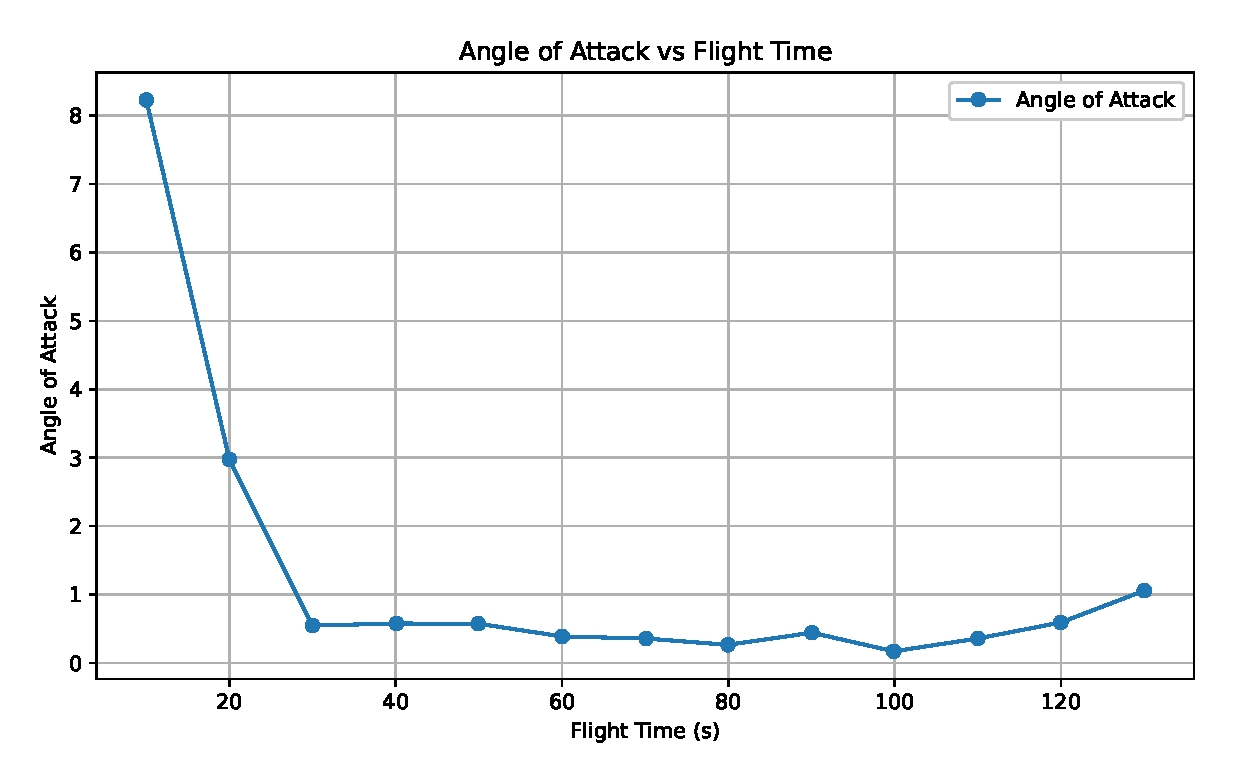
\includegraphics[width=0.495\linewidth]{figs/eris/S123F/AngleofAttack.eps}
    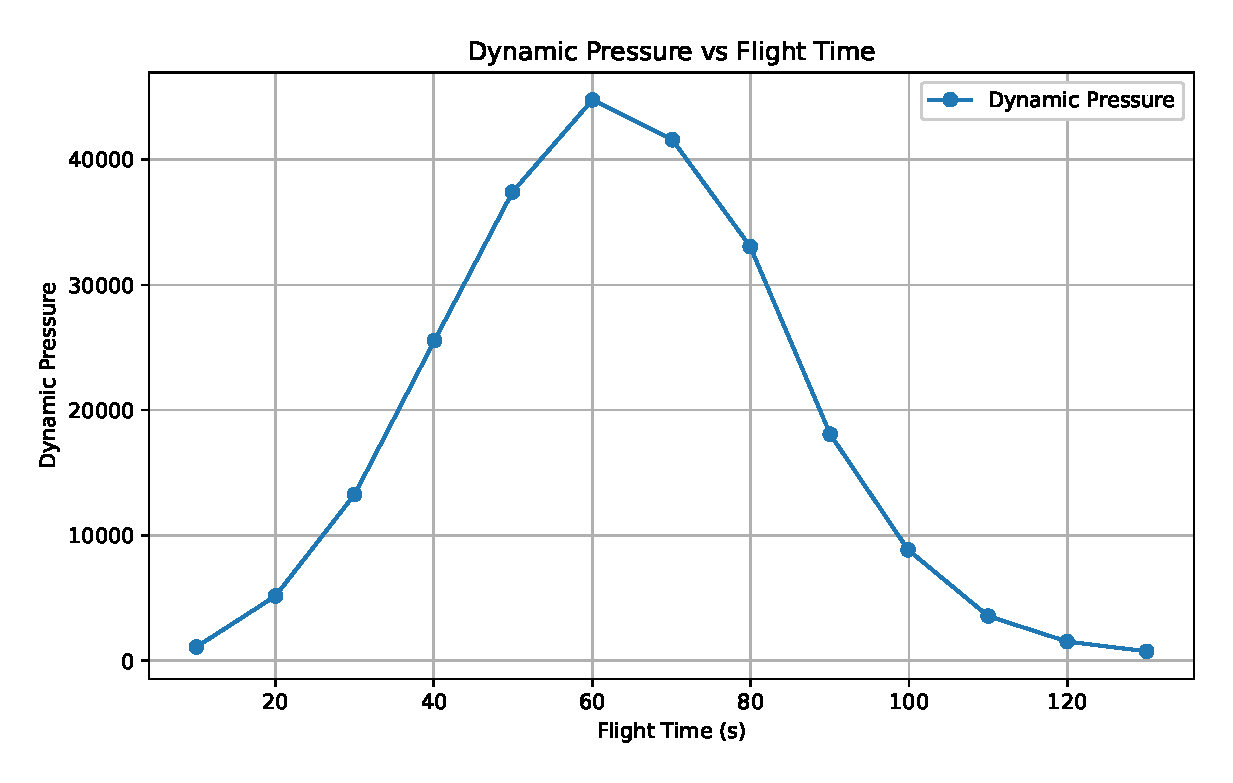
\includegraphics[width=0.495\linewidth]{figs/eris/S123F/DynamicPressure.eps}\\
    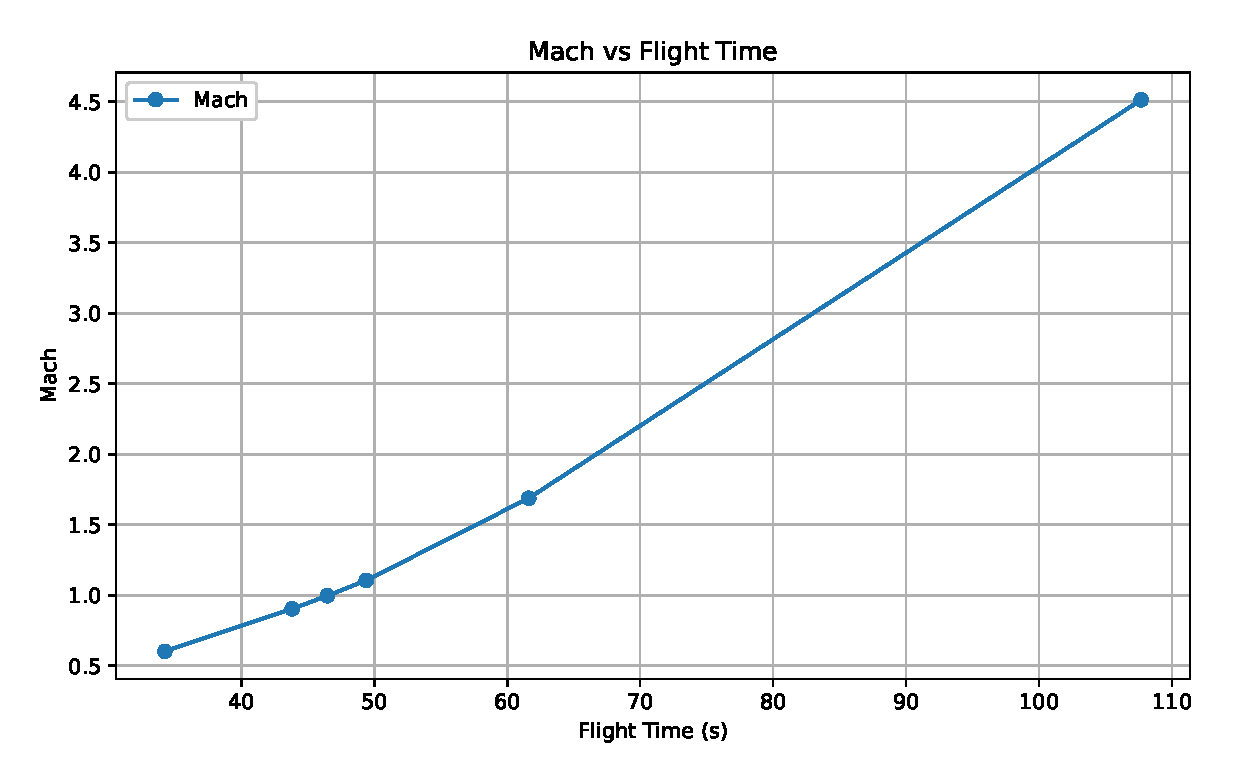
\includegraphics[width=0.495\linewidth]{figs/eris/S123F/Mach.eps}
    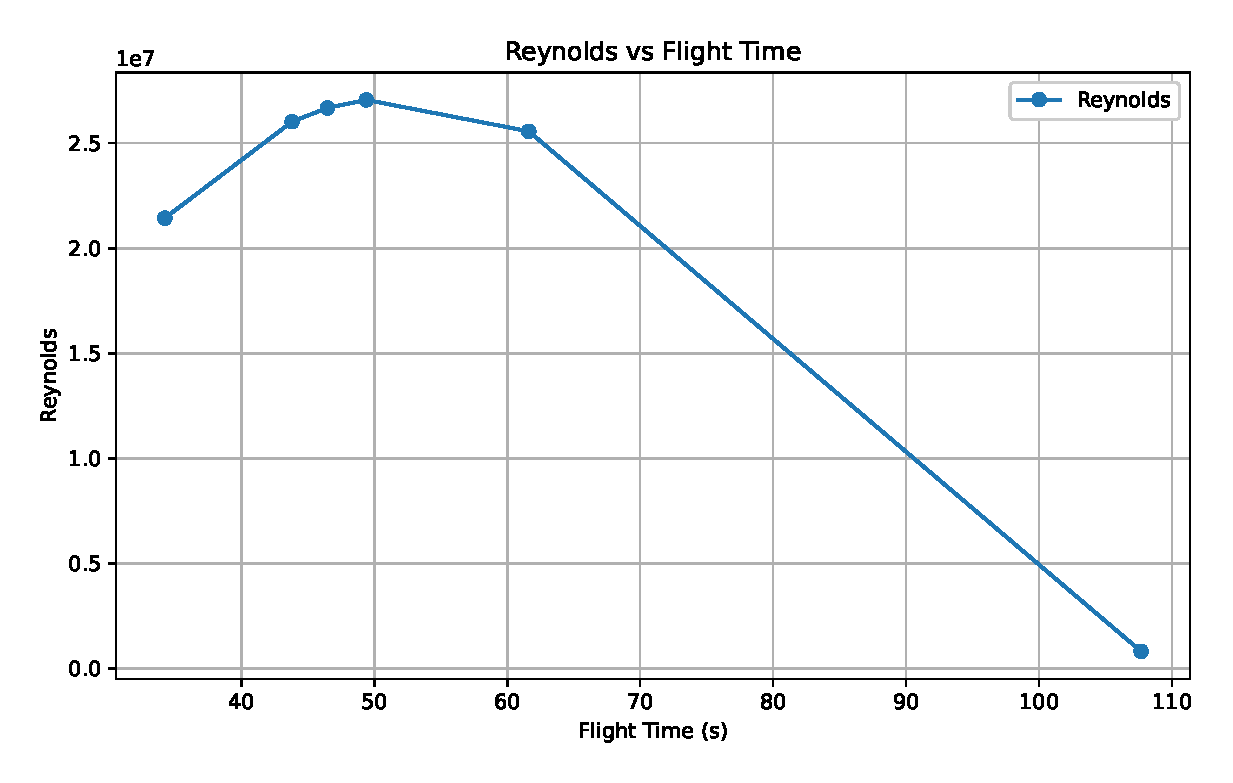
\includegraphics[width=0.495\linewidth]{figs/eris/S123F/Reynolds.eps}\\
    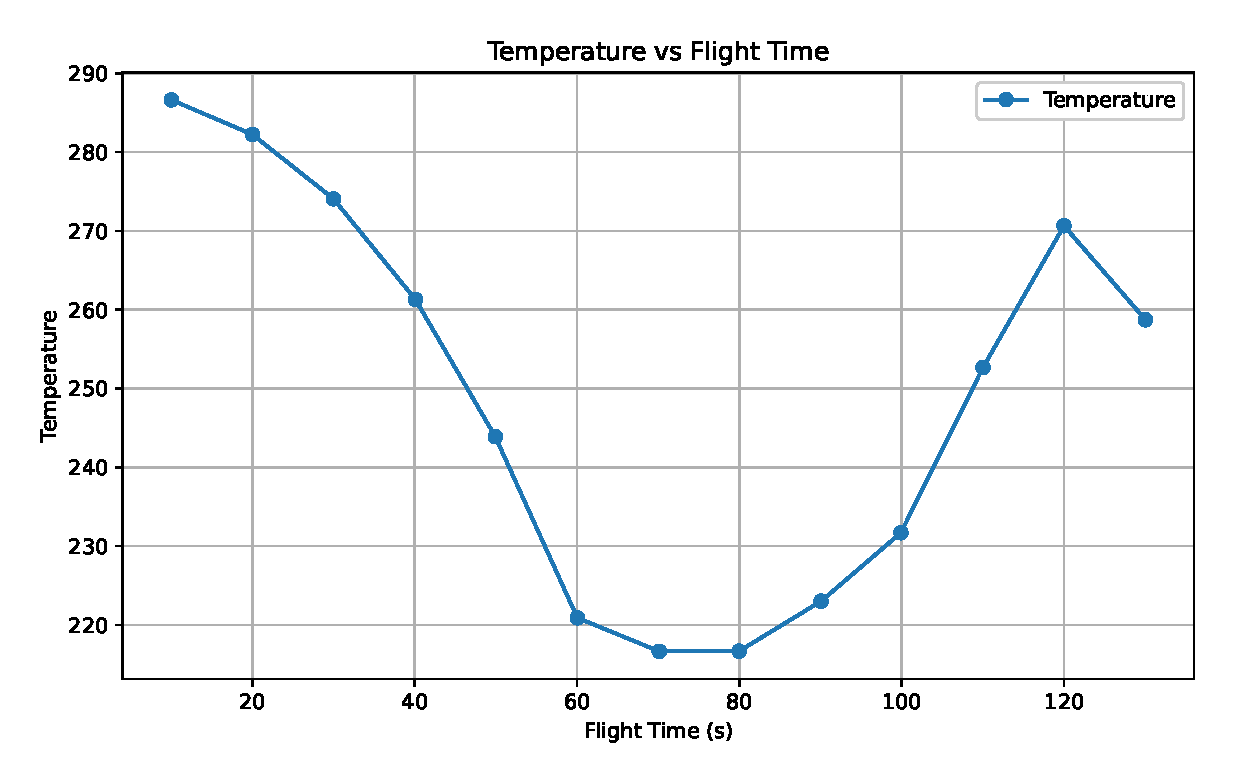
\includegraphics[width=0.495\linewidth]{figs/eris/S123F/Temperature.eps}
    %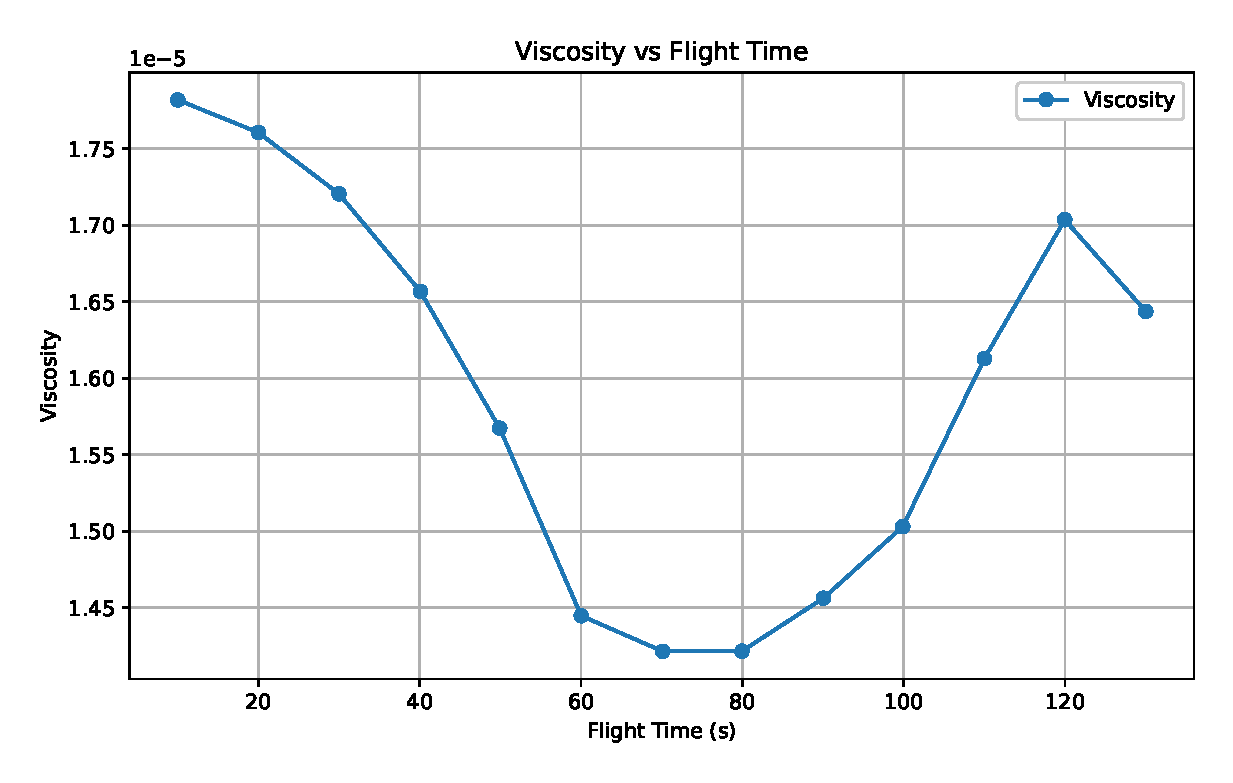
\includegraphics[width=0.495\linewidth]{figs/eris/S123F/Viscosity.eps}\\
    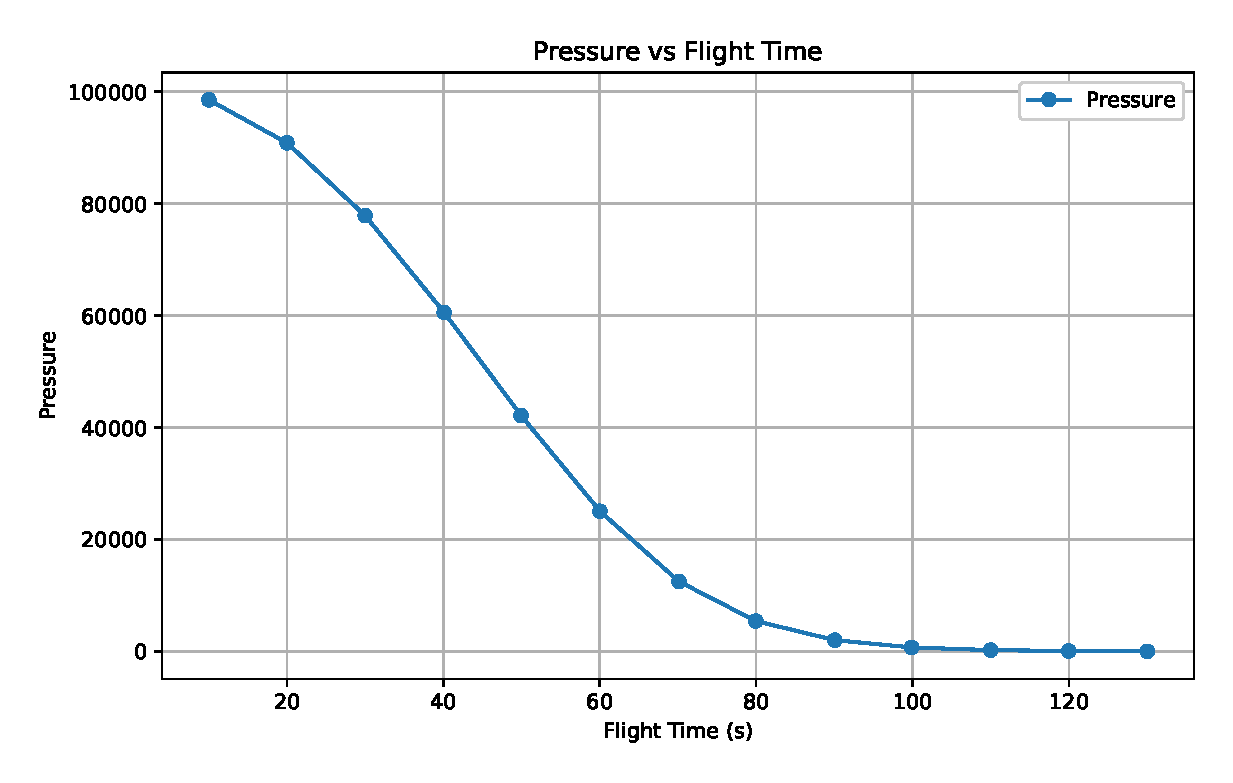
\includegraphics[width=0.495\linewidth]{figs/eris/S123F/Pressure.eps}\\
    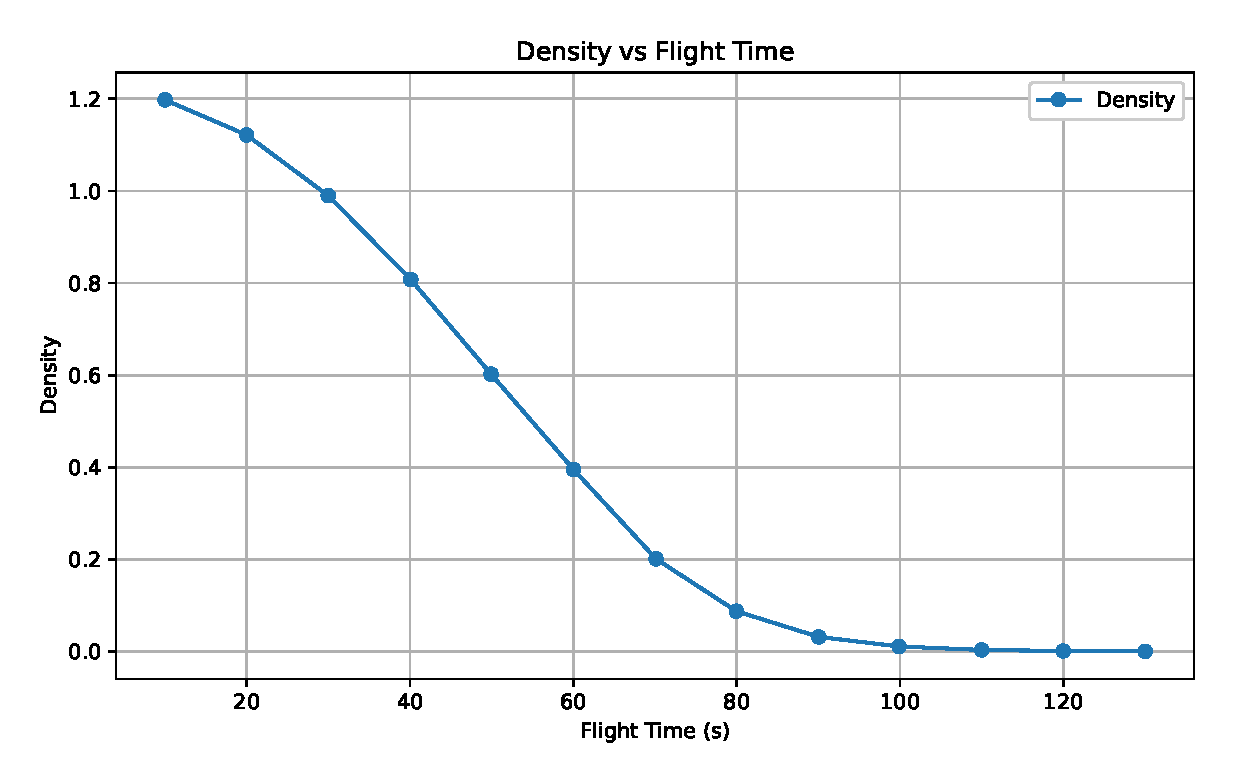
\includegraphics[width=0.495\linewidth]{figs/eris/S123F/Density.eps}
    %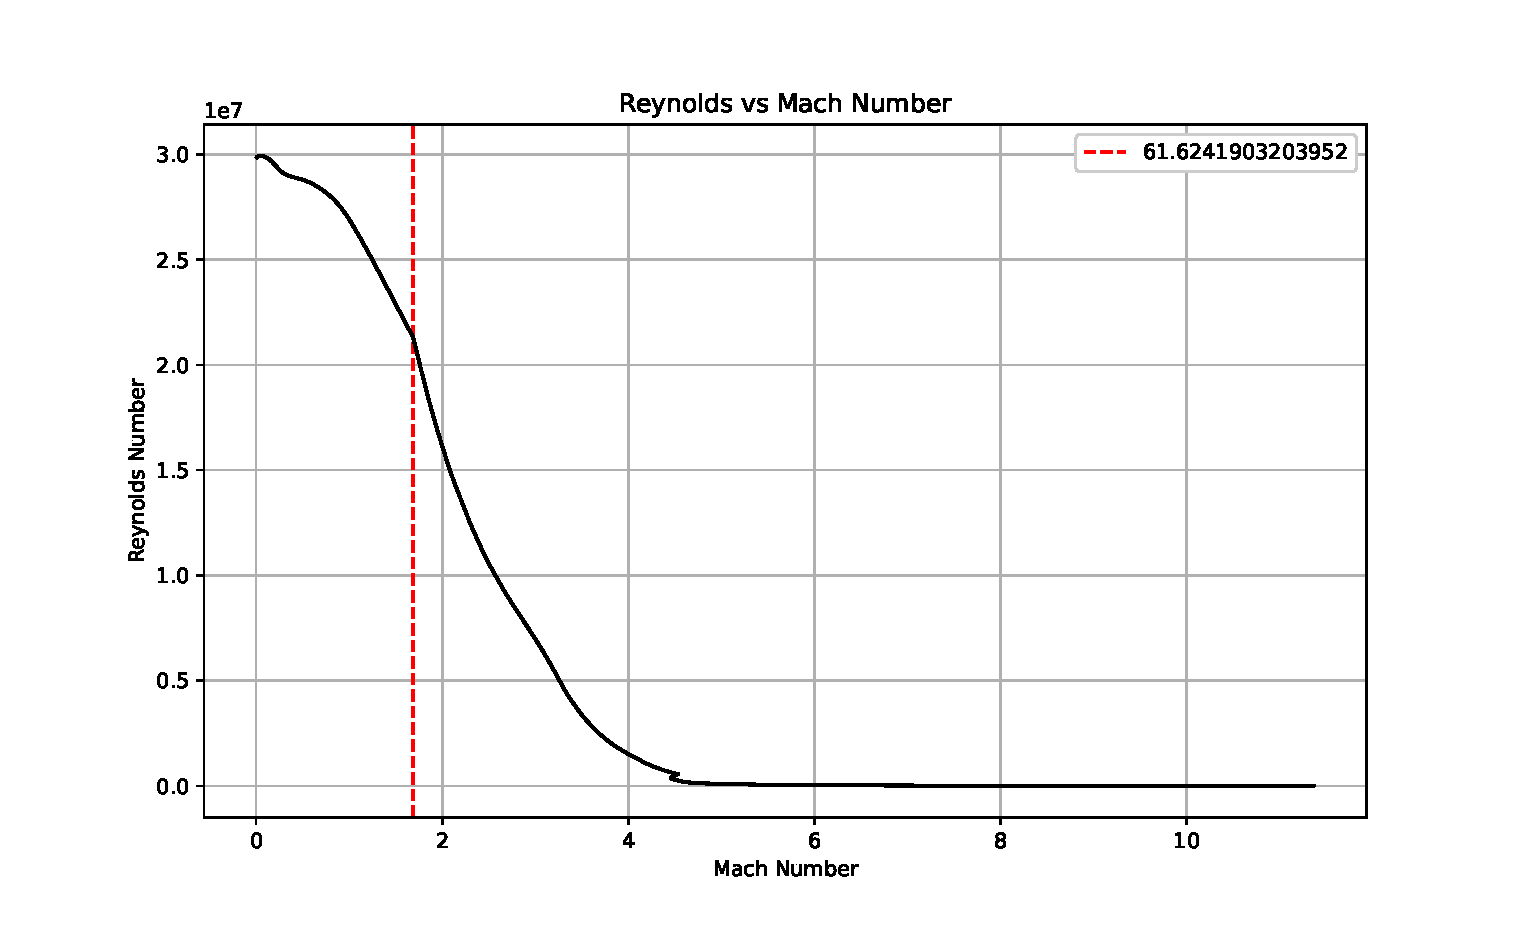
\includegraphics[width=0.495\linewidth]{figs/eris/S123F/ReVsMach.eps}
    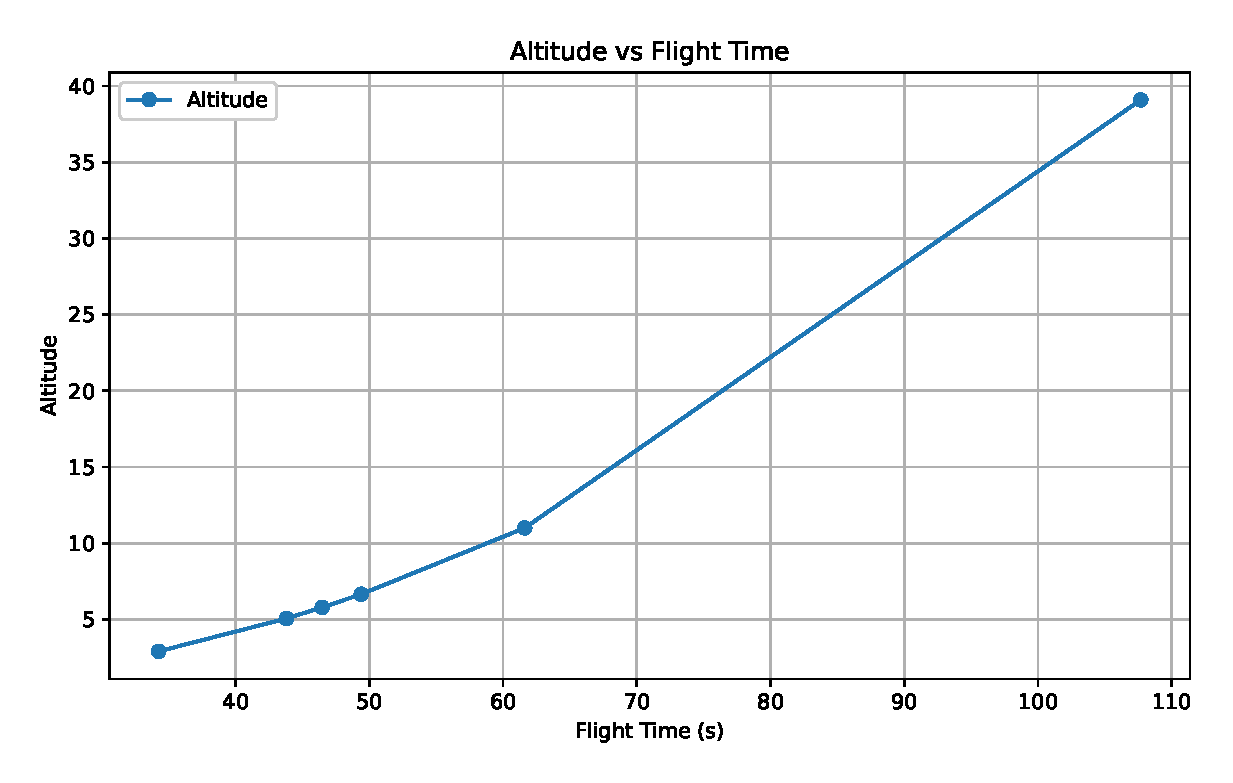
\includegraphics[width=0.495\linewidth]{figs/eris/S123F/Altitude.eps}
    \caption{Trend of several fields in time. Only few points of the flight trajectory have been plotted.}
    \label{fig:fields}
\end{figure}
%
\noindent Figure~\ref{fig:axes} shows the orientation of the LV with respect to the selected 
reference of frame. Consistently, Listing~\ref{lst:dirs} reports the convention adopted for the
sign of forces and moments for all simulations. As done for ARCAS, the pitching moment is considered positive when generates a "nose-up" motion. Differently from ARCAS, in Eris the moments are computed with respect to the base location ($x$ = 0.0).
%
\begin{figure}[H]
    \centering
    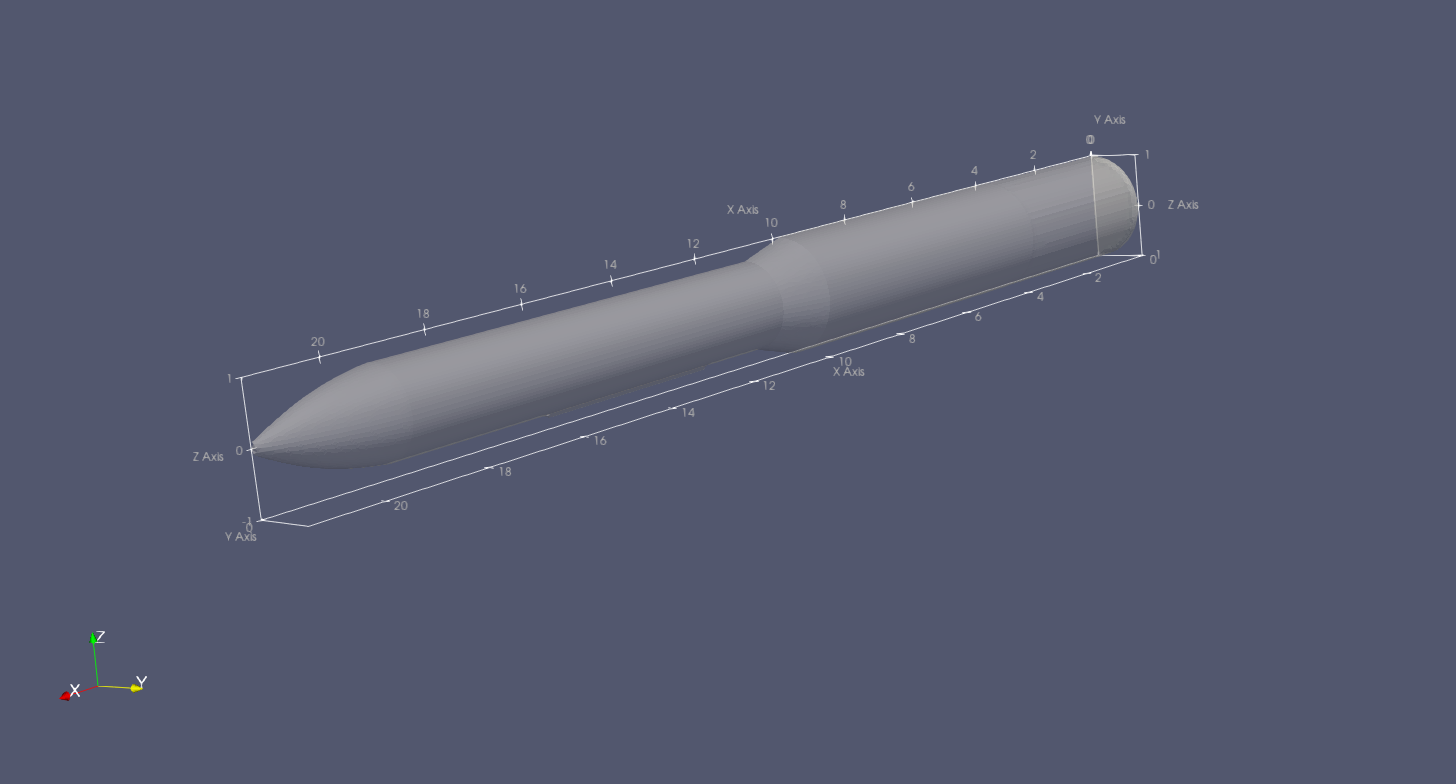
\includegraphics[width=0.99\linewidth]{figs/eris/axis-orientation.png}
    \caption{Coordinate axes orientation.}
    \label{fig:axes}
\end{figure}
%
\begin{lstlisting}[caption=Definition of the aerodynamic directions in the file system/FOs/FOforceCoeffs., label=lst:dirs, language=C++]
// Centre of rotation for moment calculations
CofR            (0 0 0);

// Lift direction
liftDir         (0 0 1);

// Drag direction
dragDir         (-1 0 0);

// Pitch axis
pitchAxis       (0, -1, 0);
\end{lstlisting}

\section{Aerodynamic database building. \textcolor{red}{\textbf{(Not applicable)}}}
%%%%%%%%%%%%%%%%%%%%%%%%%%%%%%%%%%%%%%%%%%%%%%%%%%%%%%%%%%%%%%%%%%%%%%%%%%%%%%%%%%%
One way to generate the aero-database (AEDB) is by means of a build-up approach used for both the coefficients and the uncertainties levels. The output of the AEDB is constituted by the six aerodynamic coefficients (global, lumped and distributed) and the pressure distribution: $C_L$, $C_D$, $C_S$, $C_{Mx}$, $C_{My}$, $C_{Mz}$, p=p(surface). The independent variables are: Mach number, angle of attach, Reynolds number, roll angle. Each aerodynamic contribution is a summation of several contributions and each of this contribution is function of one or more variables. In particular, we have for each Mach range the following formulas:
%
\begin{align}
C_{i,N}^{F_L}(\alpha, M, Re, \varphi, nozzle) &= \qquad \text{(Nominal generic coefficient in flight cond.)} \\
C_{i,WT}(\alpha, M) &+ \qquad \text{(Clean contr.)} \\
\Delta C_{i,WT}^{Prot}(\alpha, M, \varphi) &+ \qquad \text{(Protusion contr.)} \\
\Delta C_{i,base}^{CFD}(\alpha, M) &+ \qquad \text{(Base contr. CFD)} \\
\Delta C_{i,nozzle}^{CFD}(\alpha, M, nozzle) &+ \qquad \text{(Canted Nozzle contr. CFD)} \\
\Delta C_{i,Re}^{CFD}(\alpha, M, Re) & \quad \ \qquad \text{(Re effect (Extrapolation to flight))}
\end{align}
%
\paragraph{\textbf{Sub-transonic-Supersonic Range (M = 0.5 – 3.5)}}
\begin{align}
C_{i,\text{NFL}}(\alpha, M, Re, \varphi) &= \qquad \text{(Generic coefficient in flight cond.)} \\
C_{i,\text{WT}}(\alpha, M) &+ \qquad \text{(Nominal Wind Tunnel contribution)} \\
\Delta C_{i,\text{WTProt}}(\alpha, M, \varphi) &+ \qquad \text{(Wind Tunnel Protrusion contribution)} \\
\Delta C_{i,\text{baseCFD}}(\alpha, M, \varphi) &+ \qquad \text{(Base contribution (CFD))} \\
\Delta C_{i,\text{ReCFD}}(\alpha, M, Re) & \quad \ \qquad \text{(Re effect (Extrapolation to flight))}
\end{align}
%
\paragraph{\textbf{Hypersonic Range (M = 3.5 – 7.0)}}
\begin{align}
C_{i,\text{NFL}}(\alpha, M, Re, \varphi) &= \qquad \text{(Generic coefficient in flight cond.)} \\
C_{i,\text{CFD}}(\alpha, M) &+ \qquad \text{(CFD contribution)} \\
\Delta C_{i,\text{CFDProt}}(\alpha, M, \varphi) & \quad \ \qquad \text{(CFD Protrusion contribution)}
\end{align}
%
\paragraph{\textbf{Final Coefficient with Uncertainty Contribution}}
\begin{align}
C_{i,\text{FL}}(\alpha, M, Re, \varphi) &= \qquad \text{(Generic coefficient in flight conditions)} \\
C_{i,\text{NFL}}(\alpha, M, Re, \varphi) &+ \qquad \text{(Nominal flight contribution)} \\
\Delta C_{i,\text{UNC}}(\alpha, M, Re, \varphi) & \quad \ \qquad \text{(Uncertainty contribution)}
\end{align}
%
\paragraph{\textbf{Uncertainty for Sub-transonic-Supersonic Range}}
\begin{align}
\Delta C_{i,\text{UNC}}(\alpha, M, Re, \varphi) &= \qquad \text{(Total uncertainty contribution)} \\
\Delta C_{i,\text{UNC,WT}}(\alpha, M, Re, \varphi) &+ \qquad \text{(Wind Tunnel uncertainty contribution)} \\
\Delta C_{i,\text{UNC,CFD}}(\alpha, M, Re, \varphi) & \quad \ \qquad \text{(CFD uncertainty contribution)}
\end{align}
%
\paragraph{\textbf{Uncertainty for Hypersonic Flow Regime}}
\begin{align}
\Delta C_{i,\text{UNC}}(\alpha, M, Re, \phi) &= \qquad \text{(Total uncertainty contribution)}\label{eq:hyp1} \\
\Delta C_{i,\text{UNC,WTvsCFD}}(\alpha, M, Re, \varphi) &+ \qquad \text{(Uncertainty due to unavailability of Exp. data)}\label{eq:hyp2} \\
\Delta C_{i,\text{UNC,CFD}}(\alpha, M, Re, \varphi) & \quad \ \qquad \text{(CFD uncertainty contribution)}\label{eq:hyp3}
\end{align}
%
It should be noted that several terms are not currently available for the Eris Block 1.1 Rev. A configuration launch vehicle. In particular, terms related to wind tunnel (WT) tests should not be considered. A confidence level is required for each coefficient. This can be obtained by adding the dispersion contribution to the uncertainty value derived as described above. The dispersion contribution accounts for the \textbf{repeatability of experimental measurements} and the \textbf{non-perfect equivalence of models with the real world} in terms of geometry and far-field conditions. This contribution must be considered for CFD modeling as well, since the CAD model does not capture all geometrical details, and the far-field conditions of the numerical simulation may differ from actual flight conditions. Again, whenever experimental data is not available, the dispersion contribution should be simplified accordingly. In particular, the uncertainty reported in the above formulation takes into account two kinds of contributions:
%
\begin{itemize}
    \item Uncertainties:
    \begin{itemize}
        \item WT balance $\text{\sffamily X}$
        \item WT corrections $\text{\sffamily X}$
        \item CFD grid $\checkmark$
        \item CFD modeling $\checkmark$
        \item CFD-NoExp (unavailability of experimental data) $\checkmark$
    \end{itemize}
    \item Dispersion:
    \begin{itemize}
        \item WT balance $\text{\sffamily X}$
        \item WT repeatability $\text{\sffamily X}$
        \item Difference of WT model and/or testing wrt flight conditions $\text{\sffamily X}$
        \item Difference of CFD model and/or running wrt flight conditions $\text{\sffamily X}$
    \end{itemize}
\end{itemize}
 %
The CFD-NoExp term accounts for the lack of experimental data, such as the absence of base drag measurements and measurements with a canted nozzle. The discrepancy between the models and the real world is accounted for by incrementing the basic uncertainties by an agreed-upon percentage (5\%), typically defined with the client. It turns out that in the current conditions we cannot define dispersion. 

The confidence level comprises \textbf{uncertainties} and \textbf{dispersion}, accounting for grid sensitivity, flow modeling, and the differences between CAD models and real-world conditions. Uncertainties were calculated using correlation and variance-based error propagation. This concept is applicable for both experimental and computational values. The experimental uncertainty is linked to direct measurements (balance) and the dispersion is linked to the repeatability of the same measurements and to additional dispersions due to the differences  between the model/model-settings and the real flight conditions. Analogously the numerical uncertainty is due to the grid sensitivity and flow modeling (i.e. turbulence modeling) and the dispersion concerns with the difference between CAD model/run settings and the real world. 
%This last term is taken into account for both experiments and CFD with a suitable factor. 
The final confidence level is a summation of the experimental contribution (balance and repeatability) and numerical contribution (grid and modeling). 

The center of pressure is a derived quantity of Pitching Moment $C_{My}$ and Normal Force $C_{N}$ and is strictly correlated to them:

\paragraph{\textbf{Center of Pressure} $X_{cp}$ \textbf{Calculation}}:
%
\begin{equation}
   X_{cp} = - \frac{C_{My}}{C_{N}} \times L_{\text{ref}}
\end{equation}

\paragraph{\textbf{Uncertainty for Centre of Pressure}$(U_{Xcp}$)}:
\begin{equation}
   U_{Xcp} = \sqrt{U_{CMy}^2 + U_{CN}^2 - 2 \times \text{Corr} \times U_{CMy} \times U_{CN}}
\end{equation}

\paragraph{\textbf{Correlation} \( \text{Corr} \) \textbf{Calculation}}:
\begin{equation}
   \text{Corr} = \frac{\text{Covariance}(C_{N}, C_{My})}{\sigma_{C_N} \times \sigma_{C_{My}}}
\end{equation}

\paragraph{\textbf{Covariance Calculation}}:
\begin{equation}
   \text{Covariance}(x, y) = \frac{1}{N} \sum (x_i - \overline{x}) \times (y_i - \overline{y})
\end{equation}

\paragraph{\textbf{Variance Calculation}}:
\begin{equation}
    \sigma(x) = \sqrt{\text{Variance}(x)} = \sqrt{\frac{1}{N} \sum (x_i - \overline{x})^2}
\end{equation}

\noindent A value of 0.9 is used and is based on available data of VEGA C repeatability measurements of wind tunnel. The formula is a direct consequence of the propagation error theory. The correlation is a non-dimensional value that ranges from zero (no correlation and higher value of uncertainty) to one (full correlation and lower value of uncertainty). From the above formula we can see that in the particular case of equal values of uncertainties for $C_{My}$ and $C_N$ and full correlation (corr = 1) we can have a null uncertainty for $X_{cp}$.

\textcolor{red}{The procedure for the aerodynamic database generation outlined in this section was not followed. It was reported because it may be incorporated once experimental and flight data will be available.}

\section{Methodology}\label{sec:method}
%%%%%%%%%%%%%%%%%%%%%%%%%%%%%%%%%%%%%%%
In this section, different aspects of the methodology adopted to perform the aerodynamic characterization of the Eris Block 1.1 Rev. A configuration launch vehicle are detailed, such as the selection of the numerical solvers and their parameters' settings, grid convergence analysis, and other modeling choices (turbulence, ICs, BCs).

\subsection{Effect of grid resolution}
%%%%%%%%%%%%%%%%%%%%%%%%%%%%%%%%%%%%%%
%The effect of the grid resolution on computed results has been analyzed for the flight configuration in motor-off conditions across subsonic (M = 0.6, $\alpha$ = 0.31$^\circ$), transonic (M = 0.90, $\alpha$ = 0.65$^\circ$), supersonic (M = 1.10, 1.67, $\alpha$ = 0.55$^\circ$, 0.43$^\circ$) and hypersonic (M = 4.51, $\alpha$ = 0.12$^\circ$) regimes. Tables~\ref{tab:grid_resolution} reports the aerodynamic coefficients $C_A$, $C_N$, $C_M$, and the normalized center of pressure $X_{CP}/D$ as a function of the grid resolution, all the values having been normalized to the finest grid level ($R_2$). The coarse grid ($R_0$) results for the subsonic case have been obtained with laminar flow assumption and motor-off conditions (a strategy used to initialize the complex base flow structure), and then have to be considered only as reference values. The percentage variation between the results of the fine ($R_2$) and medium ($R_1$) grid levels is ? for the normal force, ? for the axial force, ? for the pitching moment coefficient, and ? for the position of center of pressure. 

%Concerning the supersonic case, the coarse level of the grid ($R_0$) was not adequate to capture the quite strong bow shock wave around the launcher’s nose. An intermediate grid ($R_{1,2}$) between the medium ($R_1$) and the fine ($R_2$) level of the grid has been then generated to demonstrate the grid-independence of the results. For each elementary edge an intermediate number of points between those of $R_1$ and $R_2$ levels has been selected, with the spacing law scaled accordingly. Figure~\ref{} shows the aerodynamic coefficients as a function of the parameter $h$, where N is the number of cells of a grid level, this number representing the grid resolution (the accuracy of the grid increasing from right to left). The percentage variation between the result obtained on the fine ($R_2$) and intermediate ($R_{1,2}$) grid levels is ? for the normal, ? for the axial force coefficients, ? for the pitching moment, and ? for the position of the center of pressure. The level of convergence of the solution can be estimated by using the Richardson extrapolation method  applied to functionals such as the global aerodynamic coefficients. The values of $C_N$, $C_A$, and $C_M$ have been extrapolated to zero grid spacing (h = 0) assuming the actual grid refinement ratio and a second order of accuracy. The discretization error of the CFD data has been evaluated looking at the difference between the quantitative results obtained on the fine grid level and the values extrapolated at h = 0. The error is of order of magnitude ? for both $C_N$ and $C_A$, and larger for $C_M$ (it is to be noted that the pitching moment coefficient is computed with respect to the nose-tip). It is possible to affirm that, in the frame of the physical and numerical modeling adopted in the present analysis, the computational grids employed in the simulations in subsonic, transonic, supersonic and hypersonic regimes provide grid-independent results in terms of global aerodynamic coefficients.
%
\noindent The grid meshes were generated using the same strategy adopted and explained in the \href{https://www.overleaf.com/read/ghcdhphkgfxf#df14d5}{ARCAS validation testcase report}. Shortly, .stl files were exported directly from the CAD model and then the mesh generation applies to it, according to the steps highlighted in the Listing~\ref{lst:meshgen}.
%
\begin{lstlisting}[caption=Mesh generation script., label=lst:meshgen, language=Bash]
#!/bin/sh
cd "${0%/*}" || exit 1 
. "$WM_PROJECT_DIR/bin/tools/RunFunctions"

surfaceConvert eris_original.stl eris.stl -clean -scale 0.001
runApplication surfaceGenerateBoundingBox eris.stl geometry.stl 80 60 0 40 40 40
runApplication surfaceFeatureEdges -angle 1 geometry.stl geometry.fms
runApplication -overwrite "$(getApplication)"
touch case.foam
runApplication -overwrite checkMesh -allTopology -allGeometry
runApplication -overwrite createPatch -overwrite
\end{lstlisting}
%
\noindent These grids were then converted into (.msh ASCII) \texttt{Fluent} format using the utililty application \texttt{FoamMeshToFluent}. The final (converged) \texttt{OpenFOAM} solution for each grid level was converted using \texttt{foamDataToFluent}. Then, the \texttt{Fluent} simulation was initialized with it, greatly speeding up convergence. \textbf{It is worth observing that \texttt{Fluent} simulation were not performed for the purpose of this report. Only the \texttt{OpenFOAM} solver was used to generate solutions, according to the methodology detailed in the aforementioned ARCAS report.} 

As done for ARCAS validation testcase, Equation~\ref{eq:delta} was used to calculate the turbulent boundary layer thickness ($\delta$) along a flat plate channel. It results in a $\delta$ $\approx$ 2.5 cm for the most stringent Reynolds number and a reference diameter $D$ = 2 m. Based on this result, it is estimated that the smallest cell element should have a size on the order of 2.5 cm to obtain $y^+_\text{max} < 1$. Details of the grids used for the simulations are given in Table~\ref{tab:grid_resolution}. The characteristics of the grids and of the mesh generation process are the same as those used in ARCAS, so no further details are given here.
%
\begin{equation}
    \delta = 0.37 \frac{D}{Re^{1/5}}\label{eq:delta}
\end{equation}

\begin{table}[H]
    \centering
    \captionsetup{skip=1pt} 
    \caption{Grids convergence analysis.}
    %\caption{Grids' characteristics.}
    \begin{tabular}{ccccccc}
        \hline
        \textbf{Grid Level} & \textbf{Points} & \textbf{Cells} & \textbf{C\textsubscript{A}} & \textbf{C\textsubscript{N}} & \textbf{C\textsubscript{M}} & \textbf{X\textsubscript{CP}/D} \\
        \hline 
        $R_0$ & 178445  & 177773  & - & - & - & - \\
        $R_1$ & 472686  & 459613  & - & - & - & - \\
        $R_2$ & 1720742 & 1621431 & - & - & - & - \\
        $R_3$ & 6565372 & 5782419 & - & - & - & - \\
        \hline
    \end{tabular}
    \label{tab:grid_resolution}
\end{table}
%
\noindent In practical terms, this means that at meshing time a boundary layer patch refinement should be applied, as for example shown in the Listing~\ref{lst:BLref}, ensuring that the \texttt{maxFirstLayerThickness} is as desired ($\approx$ 2 cm). Additional information about the adopted meshing tool, \texttt{Cfmesh}, can be found in the training presentation slides~\footnote{\url{https://www.wolfdynamics.com/training/CFMESH/cfmesh2017.pdf}}.
%
\begin{lstlisting}[caption=Boundary layer refinement strategy in system/\texttt{meshDict}., label=lst:BLref, language=C++]
boundaryLayers
{
    thicknessRatio 1.2;
    nLayers 0;

    patchBoundaryLayers
    {
        "S1.* S2.* S23.* S3.* NOSE.* Raceway.*"
        {
            nLayers 9;
            thicknessRatio 1.1;
            maxFirstLayerThickness 0.02; // 2 cm
            allowDiscontinuity 1;
        }
    }
}
\end{lstlisting}

It is important to note that old grid meshes and solutions are available in:
\begin{verbatim}
    V:\01 - Analysis Cold Storage (NO SAVED RESULTS)\
    Legacy Archives\Matthew.Pengelly\Eris 1.1 Ascent\
    Ascent - Eris 1.5\Saves\Max Q
\end{verbatim}
 It may be worth using exactly these meshes, after conversion, to reduce the number of parameters which could make a difference.

%% Options for packages loaded elsewhere
%\PassOptionsToPackage{unicode}{hyperref}
%\PassOptionsToPackage{hyphens}{url}
%
%\documentclass[
%]{article}
%\usepackage{amsmath,amssymb}
%\usepackage{lmodern}
%\usepackage{iftex}
%\ifPDFTeX
%  \usepackage[T1]{fontenc}
%  \usepackage[utf8]{inputenc}
%  \usepackage{textcomp} % provide euro and other symbols
%\else % if luatex or xetex
%  \usepackage{unicode-math}
%  \defaultfontfeatures{Scale=MatchLowercase}
%  \defaultfontfeatures[\rmfamily]{Ligatures=TeX,Scale=1}
%\fi
%% Use upquote if available, for straight quotes in verbatim environments
%\IfFileExists{upquote.sty}{\usepackage{upquote}}{}
%\IfFileExists{microtype.sty}{% use microtype if available
%  \usepackage[]{microtype}
%  \UseMicrotypeSet[protrusion]{basicmath} % disable protrusion for tt fonts
%}{}
%\makeatletter
%\@ifundefined{KOMAClassName}{% if non-KOMA class
%  \IfFileExists{parskip.sty}{%
%    \usepackage{parskip}
%  }{% else
%    \setlength{\parindent}{0pt}
%    \setlength{\parskip}{6pt plus 2pt minus 1pt}}
%}{% if KOMA class
%  \KOMAoptions{parskip=half}}
%\makeatother
%\usepackage{xcolor}
%\usepackage{longtable,booktabs,array}
%\usepackage{calc} % for calculating minipage widths
%% Correct order of tables after \paragraph or \subparagraph
%\usepackage{etoolbox}
%\makeatletter
%\patchcmd\longtable{\par}{\if@noskipsec\mbox{}\fi\par}{}{}
%\makeatother
%% Allow footnotes in longtable head/foot
%\IfFileExists{footnotehyper.sty}{\usepackage{footnotehyper}}{\usepackage{footnote}}
%\makesavenoteenv{longtable}
%\usepackage{graphicx}
%\makeatletter
%\def\maxwidth{\ifdim\Gin@nat@width>\linewidth\linewidth\else\Gin@nat@width\fi}
%\def\maxheight{\ifdim\Gin@nat@height>\textheight\textheight\else\Gin@nat@height\fi}
%\makeatother
%% Scale images if necessary, so that they will not overflow the page
%% margins by default, and it is still possible to overwrite the defaults
%% using explicit options in \includegraphics[width, height, ...]{}
%\setkeys{Gin}{width=\maxwidth,height=\maxheight,keepaspectratio}
%% Set default figure placement to htbp
%\makeatletter
%\def\fps@figure{htbp}
%\makeatother
%\setlength{\emergencystretch}{3em} % prevent overfull lines
%\providecommand{\tightlist}{%
%  \setlength{\itemsep}{0pt}\setlength{\parskip}{0pt}}
%\setcounter{secnumdepth}{-\maxdimen} % remove section numbering
%\ifLuaTeX
%  \usepackage{selnolig}  % disable illegal ligatures
%\fi
%\IfFileExists{bookmark.sty}{\usepackage{bookmark}}{\usepackage{hyperref}}
%\IfFileExists{xurl.sty}{\usepackage{xurl}}{} % add URL line breaks if available
%\urlstyle{same} % disable monospaced font for URLs
%\hypersetup{
%  pdftitle={Examining Spatial (Grid) Convergence},
%  hidelinks,
%  pdfcreator={LaTeX via pandoc}}
%
%\title{Examining Spatial (Grid) Convergence}
%\author{}
%\date{}
%
%\begin{document}
%\maketitle

\begin{longtable}[]{@{}
  >{\raggedright\arraybackslash}p{(\columnwidth - 0\tabcolsep) * \real{1.0000}}@{}}
\toprule()
\endhead
\begin{minipage}[t]{\linewidth}\raggedright
%\includegraphics{Examining Spatial (Grid) Convergence_files/title2.gif}
\href{https://www.grc.nasa.gov/www/wind/valid/homepage.html}{\textbf{V\&V
Home}} ~ ~ ~
\href{https://www.grc.nasa.gov/www/wind/valid/archive.html}{\textbf{Archive}}
~ ~ ~
\href{https://www.grc.nasa.gov/www/wind/valid/tutorial/tutorial.html}{\textbf{Tutorial}}

\hypertarget{examining-spatial-grid-convergence}{%
\subsection{Examining Spatial (Grid)
Convergence}\label{examining-spatial-grid-convergence}}

\hypertarget{introduction}{%
\subsubsection{Introduction}\label{introduction}}

The examination of the spatial convergence of a simulation is a
straight-forward method for determining the \emph{ordered}
\href{https://www.grc.nasa.gov/www/wind/valid/tutorial/errors.html}{discretization
error} in a CFD simulation. The method involves performing the
simulation on two or more successively finer grids. The term \emph{grid
convergence study} is equivalent to the commonly used term \emph{grid
refinement study}.

As the grid is refined (grid cells become smaller and the number of
cells in the flow domain increase) and the time step is refined
(reduced) the spatial and temporal discretization errors, respectively,
should asymptotically approaches zero, excluding computer round-off
error.

Methods for examining the spatial and temporal convergence of CFD
simulations are presented in the book by
\href{https://www.grc.nasa.gov/www/wind/valid/tutorial/bibliog.html\#Roach94}{Roache}.
They are based on use of Richardson\textquotesingle s extrapolation. A
summary of the method is presented here.

A general discussion of
\href{https://www.grc.nasa.gov/www/wind/valid/tutorial/errors.html}{errors
in CFD computations} is available for background.

We will mostly likely want to determine the error band for the
engineering quantities obtained from the finest grid solution. However,
if the CFD simulations are part of a design study that may require tens
or hundreds of simulations, we may want to use one of the coarser grids.
Thus we may also want to be able to determine the error on the coarser
grid.

\hypertarget{grid-considerations-for-a-grid-convergence-study}{%
\subsubsection{Grid Considerations for a Grid Convergence
Study}\label{grid-considerations-for-a-grid-convergence-study}}

The easiest approach for generating the series of grids is to generate a
grid with what one would consider \emph{fine} grid spacing, perhaps
reaching the upper limit of one\textquotesingle s tolerance for
generating a grid or waiting for the computation on that grid to
converge. Then coarser grids can be obtained by removing every other
grid line in each coordinate direction. This can be continued to create
additional levels of coarser grids. In generating the fine grid, one can
build in the \textbf{n} levels of coarser grids by making sure that the
number of grid points in each coordinate direction satisfies the
relation

\textbf{N = 2\textsuperscript{n} m + 1}

where \textbf{m} is an integer. For example, if two levels of coarser
grids are desired (i.e. fine, medium, and coarse grids) then the number
of grid points in each coordinate direction must equal \textbf{4 m + 1}.
The \textbf{m} may be different for each coordinate direction.

The \href{http://www.grc.nasa.gov/WWW/winddocs}{WIND} code has a
\href{http://www.grc.nasa.gov/WWW/winddocs/user/keywords/sequence.html}{grid
sequencing control} that will solve the solution on the coarser grid
without having to change the grid input file, boundary condition
settings, or the input data file. Further, the converged solution on the
coarser grid then can be used directly as the initial solution on the
finer grid. This option was originally used to speed up convergence of
solutions; however, can be used effectively for a grid convergence
study.

It is not necessary to halve the number of grid points in each
coordinate direction to obtain the coarser grid. \emph{Non-integer} grid
refinement or coarsening can be used. This may be desired since
\emph{halfing} a grid may put the solution out of the asymptotic range.
Non-integer grid refinement or coarsening will require the generation of
a new grid. It is important to maintain the same grid generation
parameters as the original grid. One approach is to select several grid
spacings as reference grid spacings. One should be the grid spacing
normal to the walls. Others may be spacings at flow boundaries, at
junctures in the geometry, or at zonal interfaces. Upon picking the
ratio as which the grid is to be refined or coarsened, this same ratio
is applied to these spacings. The number of grid points are then
adjusted according to grid quality parameters, such as grid spacing
ratio limits. The surface and volume grids are then generated using the
same methods as the original grid. The grid refinement ratio should be a
minimum of \textbf{r \textgreater= 1.1} to allow the discretization
error to be differentiated from other error sources (iterative
convergence errors, computer round-off, etc...).

\hypertarget{order-of-grid-convergence}{%
\subsubsection{Order of Grid
Convergence}\label{order-of-grid-convergence}}

The order of grid convergence involves the behavior of the solution
error defined as the difference between the discrete solution and the
exact solution,

%\includegraphics{Examining Spatial (Grid) Convergence_files/eq_error1.gif}

where \textbf{C} is a constant, \textbf{h} is some measure of grid
spacing, and \textbf{p} is the order of convergence. A "second-order"
solution would have \textbf{p = 2}.

A CFD code uses a numerical algorithm that will provide a
\emph{theoretical order of convergence}; however, the boundary
conditions, numerical models, and grid will reduce this order so that
the \emph{observed order of convergence} will likely be lower.

Neglecting higher-order terms and taking the logarithm of both sides of
the above equation results in:

%\includegraphics{Examining Spatial (Grid) Convergence_files/eq_logerror.gif}

The order of convergence \textbf{p} can be obtained from the slope of
the curve of \textbf{log(E)} versus \textbf{log(h)}. If such data points
are available, the slope can be read from the graph or the slope can be
computed from a least-squares fit of the data. The least-squares will
likely be inaccurate if there are only a few data points.

A more direct evaluation of \textbf{p} can be obtained from three
solutions using a constant grid refinement ratio \textbf{r},

%\includegraphics{Examining Spatial (Grid) Convergence_files/eq_porder1.gif}

The \emph{order of accuracy} is determined by the order of the leading
term of the \emph{truncation error} and is represented with respect to
the scale of the discretization, \textbf{h}. The \emph{local order of
accuracy} is the order for the stencil representing the discretization
of the equation at one location in the grid. The \emph{global order of
accuracy} considers the propagation and accumulation of errors outside
the stencil. This propagation causes the global order of accuracy to be,
in general, one degree less than the local order of accuracy. The order
of accuracy of the boundary conditions can be one order of accuracy
lower than the interior order of accuracy without degrading the overall
global accuracy.

\hypertarget{asymptotic-range-of-convergence}{%
\subsubsection{Asymptotic Range of
Convergence}\label{asymptotic-range-of-convergence}}

Assessing the accuracy of code and caluculations requires that the grid
is sufficiently refined such that the solution is in the asymptotic
range of convergence. The asymptotic range of convergence is obtained
when the grid spacing is such that the various grid spacings \textbf{h}
and errors \textbf{E} result in the constancy of \textbf{C},

\textbf{C = E / h\textsuperscript{p}}

Another check of the asymptotic range will be discussed in the section
on the grid convergence index.

\hypertarget{richardson-extrapolation}{%
\subsubsection{Richardson
Extrapolation}\label{richardson-extrapolation}}

Richardson extrapolation is a method for obtaining a higher-order
estimate of the continuum value (value at zero grid spacing) from a
series of lower-order discrete values.

A simulation will yield a quantity \textbf{f} that can be expressed in a
general form by the series expansion:

\textbf{f = f\textsubscript{h=0} + g\textsubscript{1} h +
g\textsubscript{2} h\textsuperscript{2} + g\textsubscript{3}
h\textsuperscript{3} + ...}

where \textbf{h} is the grid spacing and the functions
\textbf{g\textsubscript{1}}, \textbf{g\textsubscript{2}}, and
\textbf{g\textsubscript{3}} are independent of the grid spacing. The
quantity \textbf{f} is considered "second-order" if
\textbf{g\textsubscript{1} = 0.0}. The \textbf{f\textsubscript{h=0}} is
the continuum value at zero grid spacing.

If one assumes a second-order solution and has computed \textbf{f} on
two grids of spacing \textbf{h\textsubscript{1}} and
\textbf{h\textsubscript{2}} with \textbf{h\textsubscript{1}} being the
finer (smaller) spacing, then one can write two equations for the above
expansion, neglect third-order and higher terms, and solve for
\textbf{f\textsubscript{h=0}} to estimate the continuum value,

%\includegraphics{Examining Spatial (Grid) Convergence_files/eq_rich1.gif}

where the grid refinement ratio is:

\textbf{r = h\textsubscript{2} / h\textsubscript{1}}

The Richardson extrapolation can be generalized for a \textbf{p-th}
order methods and \textbf{r}-value of grid ratio (which does not have to
be an integer) as:

%\includegraphics{Examining Spatial (Grid) Convergence_files/eq_rich2.gif}

Traditionally, Richardson extrapolation has been used with grid
refinement ratios of \textbf{r = 2}. Thus, the above equation simplifies
to:

%\includegraphics{Examining Spatial (Grid) Convergence_files/eq_rich3.gif}

In theory, the above equations for the Richardson extrapolation will
provide a fourth-order estimate of \textbf{f\textsubscript{h=0}}, if
\textbf{f\textsubscript{1}} and \textbf{f\textsubscript{2}} were
computed using exactly second-order methods. Otherwise, it will be a
third-order estimate. In general, we will consider
\textbf{f\textsubscript{h=0}} to be \textbf{p+1} order accurate.
Richardson extrapolation can be applied for the solution at each grid
point, or to solution functionals, such as pressure recovery or drag.
This assumes that the solution is globally second-order in addition to
locally second-order and that the solution functionals were computed
using consistent second-order methods. Other cautions with using
Richardson extrapolation (non-conservative, amplification of round-off
error, etc...) are discussed in the book by
\href{https://www.grc.nasa.gov/www/wind/valid/tutorial/bibliog.html\#Roachebook}{Roache}.

For our purposes we will assume \textbf{f} is a solution functional
(i.e. pressure recovery). The \textbf{f\textsubscript{h=0}} is then as
an estimate of \textbf{f} in the limit as the grid spacing goes to zero.
One use of \textbf{f\textsubscript{h=0}} is to report the value as the
an improved estimate of \textbf{f\textsubscript{1}} from the CFD study;
however, one has to understand the caveats mentioned above that go along
with that value.

The other use of \textbf{f\textsubscript{h=0}} is to obtain an estimate
of the discretization error that bands \textbf{f} obtained from the CFD.
This use will now be examined.

The difference between \textbf{f\textsubscript{1}} and
\textbf{f\textsubscript{h=0}} is one error estimator; however, this
requires consideration of the caveats attached to
\textbf{f\textsubscript{h=0}}.

We will focus on using \textbf{f\textsubscript{1}} and
\textbf{f\textsubscript{2}} to obtain an error estimate. Examining the
generalized Richardson extrapolation equation above, the second term on
the right-hand side can be considered to be an an error estimator of
\textbf{f\textsubscript{1}}. The equation can be expressed as:

\textbf{A\textsubscript{1} = E\textsubscript{1} + O(
h\textsuperscript{p+1}, E\textsubscript{1}\textsuperscript{2})}

where \textbf{A\textsubscript{1}} is the actual fractional error defined
as:

\textbf{A\textsubscript{1} = ( f\textsubscript{1} - f\textsubscript{h=0}
) / f\textsubscript{h=0}}

and \textbf{E\textsubscript{1}} is the estimated fractional error for
\textbf{f\textsubscript{1}} defined as:

%\includegraphics{Examining Spatial (Grid) Convergence_files/eq_eerror1.gif}

where the relative error is defined as:

%\includegraphics{Examining Spatial (Grid) Convergence_files/eq_eps1.gif}

This quantity should not be used as an error estimator since it does not
take into account \textbf{r} or \textbf{p}. This may lead to an
underestimation or overestimation of the error. One could make this
quantity artificially small by simply using a grid refinement ratio
\textbf{r} close to 1.0.

The estimated fractional error \textbf{E\textsubscript{1}} is an
\emph{ordered} error estimator and a good approximation of the
discretization error on the fine grid if \textbf{f\textsubscript{1}} and
\textbf{f\textsubscript{2}} were obtained with good accuracy (i.e.
\textbf{E\textsubscript{1}\textless1}). The value of
\textbf{E\textsubscript{1}} may be meaningless if
\textbf{f\textsubscript{1}} and \textbf{f\textsubscript{h=0}} are zero
or very small relative to
\textbf{f\textsubscript{2}-f\textsubscript{1}}. If such is the case,
then another normalizing value should be used in place of
\textbf{f\textsubscript{1}}.

If a large number of CFD computations are to be performed (i.e for a DOE
study), one may wish to use the coarser grid with
\textbf{h\textsubscript{2}}. We will then want to estimate the error on
the coarser grid. The Richardson extrapolation can be expressed as:

%\includegraphics{Examining Spatial (Grid) Convergence_files/eq_rich4.gif}

The estimated fractional error for \textbf{f\textsubscript{2}} is
defined as:

%\includegraphics{Examining Spatial (Grid) Convergence_files/eq_eerror2.gif}

Richardson extrapolation is based on a Taylor series representation as
indicated in Eqn. \textbackslash ref\{eq:series\}. If there are shocks
and other discontinuities present, the Richardson extrapolation is
invalid in the region of the discontinuity. It is still felt that it
applies to solution functionals computed from the entire flow field.

\hypertarget{grid-convergence-index-gci}{%
\subsubsection{Grid Convergence Index
(GCI)}\label{grid-convergence-index-gci}}

\href{https://www.grc.nasa.gov/www/wind/valid/tutorial/bibliog.html\#Roach94}{Roache}
suggests a grid convergence index \textbf{GCI} to provide a consistent
manner in reporting the results of grid convergence studies and perhaps
provide an error band on the grid convergence of the solution. The
\textbf{GCI} can be computed using two levels of grid; however, three
levels are recommended in order to accurately estimate the order of
convergence and to check that the solutions are within the asymptotic
range of convergence.

A consistent numerical analysis will provide a result which approaches
the actual result as the grid resolution approaches zero. Thus, the
discretized equations will approach the solution of the actual
equations. One significant issue in numerical computations is what level
of grid resolution is appropriate. This is a function of the flow
conditions, type of analysis, geometry, and other variables. One is
often left to start with a grid resolution and then conduct a series of
grid refinements to assess the effect of grid resolution. This is known
as a grid refinement study.

One must recognize the distinction between a numerical result which
approaches an asymptotic numerical value and one which approaches the
true solution. It is hoped that as the grid is refined and resolution
improves that the computed solution will not change much and approach an
asymptotic value (i.e. the true numerical solution). There still may be
error between this asymptotic value and the true physical solution to
the equations.

\href{https://www.grc.nasa.gov/www/wind/valid/tutorial/bibliog.html\#Roach94}{Roache}
has provided a methodology for the uniform reporting of grid refinement
studies. "The basic idea is to approximately relate the results from any
grid refinement test to the expected results from a grid doubling using
a second-order method. The \textbf{GCI} is based upon a grid refinement
error estimator derived from the theory of generalized Richardson
Extrapolation. It is recommended for use whether or not Richardson
Extrapolation is actually used to improve the accuracy, and in some
cases even if the conditions for the theory do not strictly hold." The
object is to provide a measure of uncertainty of the grid convergence.

The \textbf{GCI} is a measure of the percentage the computed value is
away from the value of the asymptotic numerical value. It indicates an
error band on how far the solution is from the asymptotic value. It
indicates how much the solution would change with a further refinement
of the grid. A small value of \textbf{GCI} indicates that the
computation is within the asymptotic range.

The \textbf{GCI} on the fine grid is defined as:

%\includegraphics{Examining Spatial (Grid) Convergence_files/eq_gcifine1.gif}

where \textbf{F\textsubscript{s}} is a factor of safety. The refinement
may be spatial or in time. The factor of safety is recommended to be
\textbf{F\textsubscript{s}=3.0} for comparisons of two grids and
\textbf{F\textsubscript{s}=1.25} for comparisons over three or more
grids. The higher factor of safety is recommended for reporting purposes
and is quite conservative of the actual errors.

When a design or analysis activity will involve many CFD simulations
(i.e. DOE study), one may want to use the coarser grid
\textbf{h\textsubscript{2}}. It is then necessary to quantify the error
for the coarser grid. The \textbf{GCI} for the coarser grid is defined
as:

%\includegraphics{Examining Spatial (Grid) Convergence_files/eq_gcicoarse1.gif}

It is important that each grid level yield solutions that are in the
asymptotic range of convergence for the computed solution. This can be
checked by observing two \textbf{GCI} values as computed over three
grids,

\textbf{GCI\textsubscript{23} = r\textsuperscript{p}
GCI\textsubscript{12}}

\hypertarget{required-grid-resolution}{%
\subsubsection{Required Grid
Resolution}\label{required-grid-resolution}}

If a desired accuracy level is known and results from the grid
resolution study are available, one can then estimate the grid
resolution required to obtain the desired level of accuracy,

%\includegraphics{Examining Spatial (Grid) Convergence_files/eq_rstar.gif}

\hypertarget{independent-coordinate-refinement-and-mixed-order-methods}{%
\subsubsection{Independent Coordinate Refinement and Mixed Order
Methods}\label{independent-coordinate-refinement-and-mixed-order-methods}}

The grid refinement ratio assumes that the refinement ratio \textbf{r}
applies equally in all coordinate directions \textbf{(i,j,k)} for
steady-state solutions and also time \textbf{t} for time-dependent
solutions. If this is not the case, then the grid convergence indices
can be computed for each direction independently and then added to give
the overall grid convergence index,

%\includegraphics{Examining Spatial (Grid) Convergence_files/eq_gcisum.gif}

\hypertarget{effective-grid-refinement-ratio}{%
\subsubsection{Effective Grid Refinement
Ratio}\label{effective-grid-refinement-ratio}}

If one generates a finer or coarser grid and is unsure of the value of
grid refinement ratio to use, one can compute an effective grid
refinement ratio as:

%\includegraphics{Examining Spatial (Grid) Convergence_files/eq_reffective.gif}

where \textbf{N} is the total number of grid points used for the grid
and \textbf{D} is the dimension of the flow domain. This effective grid
refinement ratio can also be used for unstructured grids.

\hypertarget{example-grid-convergence-study}{%
\subsubsection{Example Grid Convergence
Study}\label{example-grid-convergence-study}}

The following example demonstrates the application of the above
procedures in conducting a grid convergence study. The objective of the
CFD analysis was to determine the pressure recovery for an inlet. The
flow field is computed on three grids, each with twice the number of
grid points in the \textbf{i} and \textbf{j} coordinate directions as
the previous grid. The number of grid points in the \textbf{k} direction
remains the same. Since the flow is axisymmetric in the \textbf{k}
direction, we consider the finer grid to be double the next coarser
grid. The table below indicates the grid information and the resulting
pressure recovery computed from the solutions. Each solution was
properly converged with respect to iterations. The column indicated by
"spacing" is the spacing normalized by the spacing of the finest grid.

%\begin{longtable}[]{@{}ccc@{}}
%\toprule()
%\endhead
%Grid & Normalized Grid Spacing & Pressure Recovery, Pr \\
%1 & 1 & 0.97050 \\
%2 & 2 & 0.96854 \\
%3 & 4 & 0.96178 \\
%\bottomrule()
%\end{longtable}

The figure below shows the plot of pressure recoveries with varying grid
spacings. As the grid spacing reduces, the pressure recoveries approach
an asymptotic zero-grid spacing value.

We determine the order of convergence observed from these results,

\textbf{p = ln{[} ( 0.96178 - 0.96854 ) / ( 0.96854 - 0.97050 ) {]} /
ln(2) = 1.786170}

The theoretical order of convergence is \textbf{p=2.0}. The difference
is most likely due to grid stretching, grid quality, non-linearities in
the solution, presence of shocks, turbulence modeling, and perhaps other
factors.

We now can apply Richardson extrapolation using the two finest grids to
obtain an estimate of the value of the pressure recovery at zero grid
spacing,

\textbf{Pr\textsubscript{h=0} = 0.97050 + ( 0.97050 - 0.96854 ) / (
2\textsuperscript{1.786170} - 1 )\\
= 0.97050 + 0.00080 = 0.97130}

This value is also plotted on the figure below.

The grid convergence index for the fine grid solution can now be
computed. A factor of safety of \textbf{F\textsubscript{S}=1.25} is used
since three grids were used to estimate \textbf{p}. The \textbf{GCI} for
grids 1 and 2 is:

\textbf{GCI\textsubscript{12} = 1.25 \textbar{} ( 0.97050 - 0.96854 ) /
0.97050 \textbar{} / ( 2\textsuperscript{1.786170} - 1 ) 100\% =
0.103083\%}

The \textbf{GCI} for grids 2 and 3 is:

\textbf{GCI\textsubscript{23} = 1.25 \textbar{} ( 0.96854 - 0.96178 ) /
0.96854 \textbar{} / ( 2\textsuperscript{1.786170} - 1 ) 100\% =
0.356249\%}

We can now check that the solutions were in the asymptotic range of
convergence,

\textbf{0.356249 / ( 2\textsuperscript{1.786170} 0.103083 ) = 1.002019}

which is approximately one and indicates that the solutions are well
within the asymptotic range of convergence.

Based on this study we could say that the pressure recovery for the
supersonic ramp is estimated to be \textbf{Pr = 0.97130} with an error
band of \textbf{0.103\%} or \textbf{0.001}.

%\includegraphics{Examining Spatial (Grid) Convergence_files/pr.gif}

\hypertarget{verify-a-fortran-program-to-perform-calculations-associated-with-a-grid-convergence-study}{%
\subsubsection{VERIFY: A Fortran program to Perform Calculations
Associated with a Grid Convergence
Study}\label{verify-a-fortran-program-to-perform-calculations-associated-with-a-grid-convergence-study}}

The Fortran 90 program
\href{https://www.grc.nasa.gov/www/wind/valid/tutorial/verify.f90}{verify.f90}
was written to carry out the calculations associated with a grid
convergence study involving 3 or more grids. The program is compiled on
a unix system through the commands:

\begin{quote}
\textbf{f90 verify.f90 -o verify}
\end{quote}

It reads in an ASCII file
(\href{https://www.grc.nasa.gov/www/wind/valid/tutorial/prD.do}{prD.do})
through the standard input unit (5) that contains a list of pairs of
grid size and value of the observed quantity \textbf{f}.

\begin{quote}
\textbf{verify \textless{}
\href{https://www.grc.nasa.gov/www/wind/valid/tutorial/prD.do}{prD.do}
\textgreater{}
\href{https://www.grc.nasa.gov/www/wind/valid/tutorial/prD.out}{prD.out}}
\end{quote}

It assumes the values from the finest grid are listed first. The output
is then written to the standard output unit (6)
\href{https://www.grc.nasa.gov/www/wind/valid/tutorial/prD.out}{prD.out}.
The output from the of \{\textbackslash tt verify\} for the results of
Appendix A are:

\begin{quote}
\begin{verbatim}
 --- VERIFY: Performs verification calculations ---
  
 Number of data sets read =  3
  
      Grid Size     Quantity
  
      1.000000      0.970500
      2.000000      0.968540
      4.000000      0.961780
  
 Order of convergence using first three finest grid 
 and assuming constant grid refinement (Eqn. 5.10.6.1) 
 Order of Convergence, p =  1.78618479
  
 Richardson Extrapolation: Use above order of convergence
 and first and second finest grids (Eqn. 5.4.1) 
 Estimate to zero grid value, f_exact =  0.971300304
  
 Grid Convergence Index on fine grids. Uses p from above.
 Factor of Safety =  1.25
  
   Grid     Refinement            
   Step      Ratio, r       GCI(%)
   1  2      2.000000      0.103080
   2  3      2.000000      0.356244
  
 Checking for asymptotic range using Eqn. 5.10.5.2.
 A ratio of 1.0 indicates asymptotic range.
  
  Grid Range    Ratio
  12 23      0.997980
  
 --- End of VERIFY ---
\end{verbatim}
\end{quote}

\hypertarget{examples-of-grid-converence-studies-in-the-archive}{%
\subsubsection{Examples of Grid Converence Studies in the
Archive}\label{examples-of-grid-converence-studies-in-the-archive}}

A grid convergence study is performed in the
\href{https://www.grc.nasa.gov/www/wind/valid/tutorial/wedge/wedge.html}{Supersonic
Wedge} case.

\hypertarget{examples-of-grid-converence-studies-in-literature}{%
\subsubsection{Examples of Grid Converence Studies in
Literature}\label{examples-of-grid-converence-studies-in-literature}}

Other examples of grid convergence studies that use the procedures
outlined above can be found in
\href{https://www.grc.nasa.gov/www/wind/valid/tutorial/bibliog.html\#Roachebook}{the
book by Roache} and the paper by
\href{https://www.grc.nasa.gov/www/wind/valid/tutorial/bibliog.html\#Steffen95}{Steffen
et al.}.

\hypertarget{nparc-alliance-policy-with-respect-to-grid-converence-studies}{%
\subsubsection{NPARC Alliance Policy with Respect to Grid Converence
Studies}\label{nparc-alliance-policy-with-respect-to-grid-converence-studies}}

For the WIND verification and validation effort, it is suggested that
the above procedures be used when conducting and reporting results from
a grid convergence study.

\begin{center}\rule{0.5\linewidth}{0.5pt}\end{center}

{Last Updated:} Wednesday, 10-Feb-2021 09:38:58 EST\\
\strut
\end{minipage} \\
\bottomrule()
\end{longtable}

\hypertarget{footer}{}
{Responsible NASA Official/Curator:}
\href{mailto:john.w.slater@nasa.gov}{John W. Slater}

{{Web Policies: }
\href{http://www.grc.nasa.gov/Doc/grcwebpolicies.html}{Web Privacy
Policy and Important Notices}}\\
{Adobe Reader Download: }
\href{http://www.adobe.com/products/acrobat/readstep2.html}{Adobe
Reader}

%\end{document} % Grid Convergence Analysis

\subsection{Directory structure}
%%%%%%%%%%%%%%%%%%%%%%%%%%%%%%%%
The directory structure is automatically generated from a template folder which contains all the configurations to be simulated. The full code of each script is given in Appendix~\ref{}.

\begin{verbatim}
.
├── cleanup.py
├── populate.py
├── run_all.sh
├── sync_remote_interactive.sh
├── sync_remote.sh
├── t107s
│   ├── rhoCentralFoam
│   ├── rhoPimpleFoam
│   └── t107s.csv
├── t34s
│   ├── rhoCentralFoam
│   ├── rhoPimpleFoam
│   └── t34s.csv
├── t43s
│   ├── rhoCentralFoam
│   ├── rhoPimpleFoam
│   └── t43s.csv
├── t46s
│   ├── rhoCentralFoam
│   ├── rhoPimpleFoam
│   └── t46s.csv
├── t49s
│   ├── rhoCentralFoam
│   ├── rhoPimpleFoam
│   └── t49s.csv
├── t61s
│   ├── rhoCentralFoam
│   ├── rhoPimpleFoam
│   └── t61s.csv
├── template
    ├── 0.orig.sub.rhoCentralFoam
    ├── 0.orig.sub.rhoPimpleFoam
    ├── 0.orig.sup.rhoCentralFoam
    ├── 0.orig.sup.rhoPimpleFoam
    ├── Allclean
    ├── Allpost
    ├── Allrun
    ├── Allrun.sl
    ├── constant
    ├── plot_coeffs.py
    ├── res.gp
    ├── save_coeffs.py
    ├── system.rhoCentralFoam
    └── system.rhoPimpleFoam
\end{verbatim}

The directory structure represents a typical case setup for computational fluid dynamics (CFD) simulations using OpenFOAM, a popular open-source solver. The root directory contains several folders representing different stages and configurations of the simulation. Below is the directory tree representation:

\begin{verbatim}
.
├── 0.orig
│   ├── alphat
│   ├── include
│   ├── k
│   ├── nut
│   ├── omega
│   ├── p
│   ├── T
│   └── U
├── 8226
│   ├── alphat
│   ├── heatTransferCoeff(T)
│   ├── k
│   ├── Ma
│   ├── nut
│   ├── omega
│   ├── p
│   ├── rDeltaT
│   ├── rho
│   ├── T
│   ├── U
│   ├── uniform
│   ├── wallHeatFlux
│   ├── wallShearStress
│   └── yPlus
├── Allclean
├── Allpost
├── Allrun
├── Allrun.sl
├── case.foam
├── constant
│   ├── polyMesh
│   ├── thermophysicalProperties
│   └── turbulenceProperties
├── extracted_coefficients_from_log.txt
├── images
├── log.postProcess
├── log.rhoCentralFoam
├── plot_coeffs.py
├── postProcessing
│   ├── forceCoeffs1
│   ├── solverInfo1
│   ├── surfaces1
│   ├── wallHeatFlux
│   ├── wallShearStress1
│   └── yPlus1
├── postprocess.sh
├── res.gp
├── save_coeffs.py
└── system
    ├── controlDict
    ├── decomposeParDict
    ├── fileUpdater
    ├── fileUpdaterControlDict
    ├── FOs
    ├── fvSchemes
    ├── fvSchemesUpWind
    ├── fvSchemesVanLeer
    ├── fvSolution
    ├── mapFieldsDict
    └── meshDict
\end{verbatim}

The directory structure is organized into several subfolders that separate the simulation setup into different stages and categories.

\begin{itemize}
    \item The 0.orig folder contains initial conditions for various fields such as temperature (T), velocity (U), pressure (p), turbulent properties (k, omega, nut), and other relevant parameters like alphat (thermal diffusivity) and include for mesh and boundary conditions. These variations cater to different solvers or conditions, such as rhoCentralFoam or rhoPimpleFoam, each representing different numerical approaches for solving the governing equations. For example:
    
    \begin{verbatim}
    0.orig/
    ├── alphat
    ├── include
    ├── k
    ├── nut
    ├── omega
    ├── p
    ├── T
    └── U
    \end{verbatim}
    
    \item The 8226 folder stores all available variable fields at the final simulation step. The name of the folder corresponds to the number of iterations performed by the solver.
    
    \begin{verbatim}
    8226/
    ├── alphat
    ├── heatTransferCoeff(T)
    ├── k
    ├── Ma
    ├── nut
    ├── omega
    ├── p
    ├── rDeltaT
    ├── rho
    ├── T
    ├── U
    ├── uniform
    ├── wallHeatFlux
    ├── wallShearStress
    └── yPlus
    \end{verbatim}
    
    \item The constant directory holds physical properties like thermophysical properties, and turbulence properties as well as the mesh files:
    
    \begin{verbatim}
    constant/
    ├── polyMesh
    ├── thermophysicalProperties
    └── turbulenceProperties
    \end{verbatim}
    
    \item The system directory contains configuration files for the solver settings, schemes, and decomposition:
    
    \begin{verbatim}
    system/
    ├── controlDict
    ├── decomposeParDict
    ├── fvSchemes
    └── fvSolution
    \end{verbatim}
    
    \item The remaining files and folders, such as log.postProcess, postProcessing, and plot\_coeffs.py, are dedicated to post-processing, visualization, and handling the results of the simulation. For instance, the postProcessing folder may contain subdirectories like:
    
    \begin{verbatim}
    postProcessing/
    ├── forceCoeffs1
    ├── solverInfo1
    ├── surfaces1
    └── wallHeatFlux
    \end{verbatim}
    
\end{itemize}

\subsection{Numerical solvers}\label{subsec:numerics}
%%%%%%%%%%%%%%%%%%%%%%%%%%%%%%%%%%%%%%%%%%%%%%%%%%%%%
For this analysis, \texttt{OpenFOAM} solvers, \textit{rhoCentralFoam} and \textit{rhoPimpleFoam} were adopted.
Details about their respective features and about the strategies put in place to run the simulations were provided in the ARCAS report and will not be repeated here.

\subsection{Heat transfer coefficient options}
%%%%%%%%%%%%%%%%%%%%%%%%%%%%%%%%%%%%%%%&&&%%%%

The heat transfer coefficient, \( h \) [W/(m\(^2\)K)], is computed as a \texttt{volScalarField} for a given set of patches. Optionally, the Nusselt number, \( \text{Nu} \), can also be output. The Nusselt number represents the ratio of convective to conductive heat transfer at a boundary in a fluid and is defined as:
%
\begin{equation}
\text{Nu} = \frac{hL}{\kappa}
\end{equation}
%
The following options are available for the \texttt{htcModel} entry, as explained in the \href{https://www.openfoam.com/documentation/guides/v2006/api/classFoam_1_1functionObjects_1_1heatTransferCoeff.html#details}{reference page} and in \href{https://caefn.com/openfoam/bc}{this page}:

\begin{center}
\begin{tabular}{@{}ll@{}}
\toprule
\textbf{Option}                     & \textbf{Description}                      \\ 
\midrule
\texttt{ReynoldsAnalogy}            & Reynold's analogy                         \\ 
\texttt{localReferenceTemperature}  & Local reference temperature               \\ 
\texttt{fixedReferenceTemperature}  & Specified reference temperature           \\ 
\bottomrule
\end{tabular}
\end{center}

where:

\begin{itemize}
    \item \( \text{Nu} \): Nusselt number
    \item \( h \): Convective heat transfer coefficient of the flow
    \item \( L \): Characteristic length that defines the scale of the physical system
    \item \( \kappa \): Thermal conductivity of the fluid
\end{itemize}

To compute the heat transfer coefficient, use the following command:
%
\begin{lstlisting}
postProcess -func "heatTransferCoeff(<field>)"
\end{lstlisting}

The following options are available for the \texttt{htcModel} entry:
% https://www.cfd-online.com/Forums/star-ccm/196879-heat-transfer-coefficient-local-specfied-y-standard.html
\begin{itemize}
    \item \textbf{ReynoldsAnalogy:} Reynolds analogy
    \begin{equation}
    h = 0.5 \, \rho_\infty \, C_{p,\infty} \, |U_\infty| \, C_f
    \label{eq:htc_reynolds}
    \end{equation}
    %
    \item \textbf{localReferenceTemperature:} Local reference temperature
    \begin{equation}
    h = \frac{q}{T_c - T_w}
    \label{eq:htc_local}
    \end{equation}
    %
    \item \textbf{fixedReferenceTemperature:} Fixed reference temperature
    \begin{equation}
    h = \frac{q}{T_c - T_{\text{ref}}}
    \label{eq:htc_fixed}
    \end{equation}
\end{itemize}

The heat transfer coefficient calculation based on the Reynolds analogy, Equation~\ref{eq:htc_reynolds}, relates turbulent momentum and heat transfer. The heat transfer coefficient is derived from the skin friction coefficient, given in \href{https://www.openfoam.com/documentation/guides/v2206/api/classFoam_1_1heatTransferCoeffModels_1_1ReynoldsAnalogy.html#details}{this page}:

\begin{equation}
C_f = \frac{\tau_w}{0.5 \rho_\infty |U|^2}
\label{eq:skin_coeff}
\end{equation}

where:
\begin{itemize}
    %\item $h$ = Convective heat transfer coefficient of the flow
    \item $\rho_\infty$ = Reference fluid density
    \item $C_{p,\infty}$ = Reference specific heat capacity at constant pressure
    \item $U_\infty$ = Reference velocity
    \item $C_f$ = Skin friction coefficient
    \item $\tau_w$ = Wall shear stress
\end{itemize}

The pressure coefficient, either static or total, from \href{https://www.openfoam.com/documentation/guides/latest/doc/guide-fos-field-pressure.html}{this page}, is given by:

\begin{equation}
C_p = \frac{p_0}{0.5 \rho_\infty |u_\infty|^2}
\label{eq:cp}
\end{equation}

where:
\begin{itemize}
    \item $C_p$ = Pressure coefficient
    \item $p_0$ = Total (or static) pressure
    \item $\rho_\infty$ = Reference fluid density
    \item $u_\infty$ = Reference velocity
\end{itemize}

\textbf{Isentropic pressure, $p_i$}:

\begin{equation}
p_i = p \left[1 + \frac{\gamma - 1}{2} M^2 \right]^{\frac{\gamma}{\gamma - 1}}
\label{eq:pi}
\end{equation}

where:

\begin{itemize}
    \item $\rho$ = Density [kg/m$^3$]
    \item $u$ = Velocity [m/s]
    \item $\rho_\infty$ = Freestream density [kg/m$^3$]
    \item $p_\infty$ = Freestream pressure [Pa]
    \item $u_\infty$ = Freestream velocity [m/s]
    \item $p_k$ = Kinematic pressure ($\frac{p}{\rho}$) [m$^2$/s$^2$]
    \item $p_s$ = Static pressure [Pa]
    \item $p_0$ = Total pressure [Pa]
    \item $p_\text{ref}$ = Reference pressure level [Pa]
    \item $p_i$ = Total isentropic pressure [Pa]
    \item $C_p$ = Pressure coefficient
    \item $C_{p0}$ = Total pressure coefficient
    \item $\gamma$ = Specific heat ratio
\end{itemize}

For incompressible cases, the kinematic pressure (pressure divided by density) can be converted to pressure via a user-specified reference density.

%https://www.openfoam.com/documentation/guides/latest/doc/guide-fos-field-heatTransferCoeff.html
\begin{lstlisting}[caption={heatTransferCoeff1 Configuration.}, label={lst:heatTransferCoeff1}, language=C++]
heatTransferCoeff1
{
    // Mandatory entries (unmodifiable)
    type            heatTransferCoeff;
    libs            (fieldFunctionObjects);
    field           <field>;
    patches         (<patch1> <patch2> ... <patchN>);
    htcModel        <htcModel>;
    UInf            (20 0 0);
    Cp              CpInf;
    CpInf           1000;
    rho             rhoInf;
    rhoInf          1.2;

    // Optional (inherited) entries
    result          <fieldResult>;
    region          region0;
    enabled         true;
    log             true;
    timeStart       0;
    timeEnd         1000;
    executeControl  timeStep;
    executeInterval 1;
    writeControl    timeStep;
    writeInterval   1;
}
\end{lstlisting}

Probably, the most straightforward solution is simply computing withing OpenFOAM the temperature gradient and the thermal conductivity from the Sutherland law or any model actually in use, as documented in \href{https://www.openfoam.com/documentation/user-guide/5-models-and-physical-properties/5.2-thermophysical-models}{this page}, and then the heat flux by the Fourier law.

% https://www.openfoam.com/documentation/guides/latest/doc/guide-bcs-common-combinations.html
\begin{table}[H]
    \centering
    \begin{tabular}{ccccc}
        \hline
        \textbf{Inlet} & \textbf{Outlet} & \textbf{Stability} \\ \hline
        %\multicolumn{2}{|c|}{\textbf{Physics}} & \multicolumn{2}{c|}{\textbf{OpenFOAM}} & \\ \hline
        Mass flow rate & flowRateVelocity & Static pressure & fixedValue & Excellent \\ \hline
        Total pressure & totalPressure & Total pressure & totalPressure & Very good \\ \hline
        Total pressure & totalPressure & Static pressure & fixedValue & Good \\ \hline
        Static pressure & fixedValue & Static pressure & fixedValue & Poor \\ \hline
    \end{tabular}
    \caption{Boundary Conditions and Stability in OpenFOAM Simulations}
    \label{tab:boundary_conditions}
\end{table}

%\begin{table}[H]
%\centering
%\captionsetup{skip=1pt} 
%\caption{OpenFOAM (OF)/Ansys Fluent (AF) Numerical Methods, Schemes, and Models.}
%\begin{tabular}{l|l|l}
%\hline
%\textbf{Category} & \textbf{AF} & \textbf{OF} \\ \hline
%\textbf{Numerical Method} & &                 \\ \hline
%Algorithm & URANS & URANS                     \\ \hline
%Method & Unstructured FVM & Unstructured FVM  \\ \hline
%Solver & Density-based  & \texttt{rhoPimpleFoam}, \texttt{rhoCentralFoam} \\ \hline
%Pressure–velocity coupling & PIMPLE & PIMPLE  \\ \hline
%Linear Algebra and Accuracy & GS/ILU, $10^{-7}$ & ICCG, $10^{-7}$ \\ \hline
%Multigrid & -- & --                           \\ \hline
%Under-relaxation Factors & Default, 0.3 (pressure), 0.7 (others) & -- \\ \hline
%\textbf{Spatial Discretization} & &          \\ \hline
%Convective Terms & QUICK & NVD, $c = 0.1$    \\ \hline
%Pressure & Standard & 4th order              \\ \hline
%\textbf{Temporal Discretization} & &         \\ \hline
%Scheme                                      & Implicit dual-stepping                         & BDF2                                 \\ \hline
%Time Step                                   & Constant $\Delta t$, CFL $<$ 1                 & Dynamic $\Delta t$, CFL $<$ 1        \\ \hline
%\textbf{Thermodynamics}                     &                                                &                                      \\ \hline
%Compressibility                             & Ideal gas law                                  & Ideal gas law                        \\ \hline
%Dynamic Viscosity, $\mu$                    & Constant, $1.7894 \times 10^{-5}$              & Constant, $1.7894 \times 10^{-5}$    \\ \hline
%Prandtl Number, $\text{Pr}$                 & Constant, 0.75                                 & Constant, 0.75                       \\ \hline
%\textbf{Turbulence Model}                   &                                                &                                      \\ \hline
%Model                                       & $k$–$\omega$ SST & $k$–$\omega$ SST \\ \hline
%Near-the-Wall Treatment                     & Low-Reynolds-number formulation                & Low-Reynolds-number formulation      \\ \hline
%\textbf{Boundary Conditions}                &                                                &                                      \\ \hline
%Inlet                                       & Fixed profiles                                 & Fixed profiles                       \\ \hline
%Outlet                                      & Pressure-far-field                             & Wave-transmissive                    \\ \hline
%Walls                                       & Isothermal, non-slip                           & Isothermal, non-slip                 \\ \hline
%\end{tabular}
%\end{table}

%\section{Experimental Activities}
%%%%%%%%%%%%%%%%%%%%%%%%%%%%%%%%%
%\colorbox{yellow}{Not available}

%\section{Extrapolation to Flight Procedure}
%%%%%%%%%%%%%%%%%%%%%%%%%%%%%%%%%%%%%%%%%%%
%The flight extrapolation was applied for Mach numbers in the sub-transonic to low supersonic range. This procedure~\cite{nicoli2005wind,vitaglianoaerodynamic,catalano2007cfd} integrated CFD Reynolds effects and base/nozzle contributions with WT experimental polars to produce flight polars.
%
%\subsection{Comparison between experiments and computations}
%%%%%%%%%%%%%%%%%%%%%%%%%%%%%%%%%%%%%%%%%%%%%%%%%%%%%%%%%%%%%
%The ground to flight extrapolation procedure is based on the use of both the experimental and the numerical data in order to identify a unique trend with Reynolds of the aerodynamic coefficients up to the flight conditions. In fact 
%generally, the experimental trends with Reynolds were acquired at three different Reynolds numbers, referred to as maximum, intermediate and minimum values. The numerical trends were evaluated at the flight condition, at the maximum wind tunnel Reynolds number and at an intermediate Reynolds number (selected in the middle between the two previous values on a logarithmic 
%scale). Nevertheless the numerical trends cannot be directly used to extend the experimental ones to the flight conditions, but a preliminary analysis of the results is needed to verify whether the two set of data can be used as a 
%single one, or if they do not match exactly between each other; in this case, it will be necessary to understand which is the reasons for the differences, in order to overcome and correct them. 
%So, the first step in the ground to flight extrapolation procedure adopted consisted in the comparison of the experimental and numerical results, both in terms of global and local coefficients at the same Reynolds number, and 
%trends with Reynolds. The causes of the inevitable small differences between the two sets of data were then identified. The necessary corrections to use all the data as a single set of information were eventually applied. 
%Once systematic error are found, the numerical trend is correct and the computational results by shifting the data of the same amount, independently from the Reynolds number at which they are computed. The magnitude of 
%the correction is determined as the difference between the experimental and numerical results evaluated at the higher wind tunnel Reynolds number.
%
%\subsection{Identification of the coefficients trends with Reynolds}
%%%%%%%%%%%%%%%%%%%%%%%%%%%%%%%%%%%%%%%%%%%%%%%%%%%%%%%%%%%%%%%%%%%%%
%Analyses like the one above made possible to treat the two sets of data as a single one. A unique trend with Reynolds, at all angles of attack at which numerical data where computed, was identified. This is shown in Figure~\ref{} where both the experimental and the corrected numerical trends with Reynolds number of the normal force coefficient at $\alpha$ = ?$\circ$ are plotted at different Mach numbers; the experimental data are reported with the error bars. 
%It should be noted the good agreement between the experimental and numerical trends. This is due to the fact that the same flow structures observed at the wind tunnel condition can be expected in flight. In fact, even in the most critical situation, like at M=0.95 where there is a strong viscous/inviscid interaction at the boat tail at wind tunnel conditions, the same interaction was numerically predicted at flight condition. 
%
%At each Mach number, the trends can be described by the following function:
%%
%\begin{equation}
%C_{N,A,M} = a [\log(Re)]^{b(M,\alpha)}
%\end{equation}
%%
%%\begin{equation}
%%C_A = a [\log(Re)]^{b(M,\alpha)}
%%\end{equation}
%%
%%\begin{equation}
%%-C_M = a [\log(Re)]^{b(M,\alpha)}
%%\end{equation}
%%
%This function has two advantages: first, it fits the data with a very good approximation, well within the experimental uncertainty bars; second, it has a simple form, in which the parameter $b$ that describes the slope of the extrapolation curves can be expressed as function of both Mach number and angle of attack. The dependence of the aerodynamic coefficients on the Reynolds number can be expressed as analytical function, and this allows to simply 
%evaluate the coefficients on trajectories that differ from the nominal one.
%
%The parameter $b$ as obtained from the trends in Figure~\ref{} is plotted as a function of Mach number in Figure~\ref{}. These curves allow to interpolate the actual value of the slope $b$ of the extrapolation function, Eq.~\ref{} and then to extrapolate at the Mach numbers at which only the coefficients at the maximum wind tunnel Reynolds number were measured and trends with Reynolds, were not available. %From this plot it can be noted that in transonic regime the Reynolds effect is almost independent from the Mach number, whereas in supersonic regime, between M=1.5 and 4, it decreases as Mach number increases, as expected. 
%
%\subsection{Dependency on the angle of attack}
%%%%%%%%%%%%%%%%%%%%%%%%%%%%%%%%%%%%%%%%%%%%%%%
%The numerical trends with Reynolds number can support the extrapolation of the aerodynamic coefficients only at $\alpha$ = ? and $\alpha$ = ? where the computations are available. In order to extrapolate in the whole range of angle of attacks of interest, (that is 0<$\alpha$<10, the range within which the aerodynamic coefficients where experimentally acquired) it can be 
%observed that only CN$\alpha$ is affected by changes in Reynolds number; in fact, the difference between the normal force coefficients measured respectively at the minimum and maximum wind tunnel Reynolds number (4) can be considered  with a good approximation a linear function of the angle of attack. 
%
%It has to be noted that $\Delta$ $C_N$ is very small, therefore any non linearity of this difference is negligible if compared with the experimental uncertainty (represented by the error bars).
%
%On the basis of the above considerations it is possible to model as linear the function $\Delta$CNfl, which represents the difference between the unknown normal force coefficient in flight and the value measured at the higher Reynolds number in wind tunnel, or in other words the correction that has to be applied to the $C_N$ measured at wind tunnel conditions to extrapolate this value at the flight conditions: 
%%
%\begin{equation}
%\Delta C_N = C_N \left( R_{emax} \right) - C_N \left( R_{fl} \right) = k \alpha
%\end{equation}
%%
%It is possible to evaluate the coefficient k by using the extrapolated values of $\Delta$CNfl already computed at ... as shown in the previous section, and the condition $\Delta$CNfl. The value of k which minimizes the deviation of the 
%function k$\alpha$ (the black straight line in Fig. 24) from the extrapolated values at 2 and 5 (black squares in Fig. 24) was computed at all Mach numbers, as it is shown in Fig. 24 for M=2. It is worthwhile noting that the extrapolated values of $\Delta$CNflat 2 and 5 are almost perfectly aligned with the origin of the axis, and this strongly supports the hypothesis expressed by (5). 
%Regarding the analysis of the pitching moment coefficient, it follows the same considerations done for CN: in fact only CM$\alpha$ changes with the Reynolds number, and the correction on $C_M$ is linear with the angle of attack. 
%A different behaviour was found for the axial force coefficient: provided that the boundary layer is fully turbulent and the flow topology is not changing with Reynolds up to the flight conditions, as it was found in subsonic and supersonic regime (see section 5), it can be expected that the scale effects, at least for the model attitudes of interest, can be mainly 
%ascribed to a reduction of the friction drag [6].
%
%\subsection{The extrapolation in hypersonic regime}\label{subsec:hyp-extrapolation}
%%%%%%%%%%%%%%%%%%%%%%%%%%%%%%%%%%%%%%%%%%%%%%%%%%%%%%%%%%%%%%%%%%%%%%%%%%%%%%%%
%In the previous section only the extrapolation in the subsonic and supersonic regimes up to M=4 has been presented: in the hypersonic regime the main hypotheses used in the extrapolation procedure in the lower Mach number range are no longer valid. In particular the error of the numerical data with respect to the experimental measurements depends upon the Reynolds number, in contrast with the previous cases. Let us consider for example Fig. ?, which is the analogous of  Fig. ? at M=? Again, there is an underestimation of the numerical vortex lift at , whilst at  the numerical results overpredict the $C_N$ with respect to the experiments.
%
%Looking at the lumped coefficients reported in Fig. ?, it can be observed that the main differences between numerical and experimental results are concentrated on the flare and on the final part of the intermediate cylinder. 
%The flow pattern found in the hypersonic regime suggests that, in this case, the differences between numerical and experimental data are caused by a slightly different prediction of the separation at the boat tail, that has a downstream effect on the shock wave intensity at the flare. Finally, it can be concluded that any correction of the numerical data in this case should be strongly Reynolds number dependent in contrast with the conclusions deducted at M=3. In other words, the numerical trends with Reynolds could be significantly misleading if used to extrapolate up to the flight conditions. 
%In addition, as already shown in Fig. ?, in the hypersonic regime the Reynolds number effects on the aerodynamic coefficients are neither linear or constant with $\alpha$ and the hypothesis expressed in (4) is not valid anymore in this regime. For these reasons, in this case the extrapolation was made using a different procedure: the aerodynamic coefficients were experimentally evaluated at six different values of Reynolds number, and since the flight conditions were close to the maximum wind tunnel Reynolds number the extrapolation was performed using only the experimental data. CFD results were only used to predict changes in the flow topology between flight and wind tunnel 
%conditions in order to support the extrapolation performed with the experimental trend. The latter was fitted with the extrapolation functions described by equations 1, 2 or 3, computed at several angles of attack and not only at 2 and 5 since the parameter $b$ is not anymore a linear or constant function of $\alpha$. 
%
\section{Results and discussion}\label{sec:results}
%%%%%%%%%%%%%%%%%%%%%%%%%%%%%%%%%%%%%%%%%%%%%%%%%%%
In this section results and discussion are provided. Numerical results obtained with three different solvers are compared, namely, \texttt{OpenFOAM}, \texttt{\st{Fluent}} and \texttt{DATCOM}. The uncertainty margins applied to these results have been estimated from the ARCAS validation testcase, as detailed in the ARCAS report (\url{https://www.overleaf.com/read/hzdjbytsxvyt#e4f8b0}). Two configurations were investigated, a full vehicle (S123F) and the vehicle without the first stage (S23F), as detailed below. Two angles of attack were considered, namely: $\alpha$ = 0$^\circ$ and $\alpha$ = 4$^\circ$ and six Mach numbers, M = 0.6, 0.9, 1, 1.1, 1.67 and 4.51. Full details about the initial conditions can be found in Table~\ref{tab:flight_trajectory} which was automatically generated from the original flight trajectory data by sampling at the desired times, and only recomputing the values of velocity and angle of attack.

%\subsection{DATCOM vs OpenFOAM vs Fluent}\label{subsec:solvers}
\subsection{Stage 1 + 2 + 3 and Fairing (S123F)}\label{subsec:solvers}
%%%%%%%%%%%%%%%%%%%%%%%%%%%%%%%%%%%%%%%%%%%%%%%%%%%%%%%%%%%%%%%%%%%%%%
This subsection reports all simulations performed for the aerodynamic characterization of the full vehicle Eris Block 1.1 Rev. A for the S123F configuration without plume effect (motor-off) using \texttt{OpenFOAM}, \texttt{\st{Fluent}} and \texttt{DATCOM}. Several points along the flight trajectory have been selected in order to possibly cover all regimes.

% Discussion here ...
%Normal, axial force, and pitching moment coefficients are reported
%in Fig. ? as functions of the Mach number, at $\alpha$ = 0, 8 and 16$^\circ$ , at
%different Reynolds numbers. The normal force coefficient, accordingly to Mach number independence principle, tends to a limit value at both the incidences. The comparison with the measured data is rather good at $\alpha$ = 0$^\circ$  except at M = 0.50 that is, however, affected by unsteady phenomena [13,16]. A systematic under-estimation of the numerical data is present at $\alpha$ = 8$^\circ$ . This is probably due to a wrong quantitative prediction of the system of the eddies detaching on the lee side of the launcher, and of the associated
%vortex lift. Limited resolution of the grid in the azimuthal direction
%and location of the far-field boundaries are the possible culprits. The
% $C_N$ results are weakly influenced by the Reynolds number.
%
%The axial force coefficient strongly depends on the base drag. In
%subsonic and transonic regimes, where the contribution of the base to
%the total drag is large, a not completely satisfactory agreement with
%the experimental data is obtained. In the supersonic regime, instead,
%the contribution of the base is not significant and a good agreement
%with the measured axial force coefficients is achieved. The drag rise
%is present in the transonic flow regime and the maximum of $C_A$ is
%reached at M = 1.20 at both the angles of attack. The Reynolds
%number has an influence on the $C_A$, but this is only due to the base, as
%the pressure distributions show. 
%
%The pitching moment coefficient has been computed with respect
%to the nose-tip of the launcher, and decreases with the Mach number
%becoming constant in the supersonic regime. The comparison
%between numerical and experimental results follows the normal
%coefficient curve because ... An oscillation,
%apparently not measured in the experiments, is present in the
%transonic CFD data.
%
%The experimental results have been reported in Fig. ? together
%with the error bars, larger in the subsonic and transonic than in the
%supersonic flow regime. The uncertainty of the $C_A$ measured at
%M = 0.50 is quite evident.

\begin{table}[H]
    \centering
    \caption{\scriptsize{Report on all simulations performed for the aerodynamic characterization of the rocket ERIS Block 1.1 Rev. A without plume effect (motor-off) using \texttt{OpenFOAM} (\textit{rhoCentralFoam} and \textit{rhoPimpleFoam}), \texttt{\st{Fluent}} and \texttt{DATCOM}. \textcolor{red}{Red} values require further iterations to converge. \textbf{Bold} values have been recalculated after checking.
    \textcolor{red}{\textbf{\ul{This table contains wrong values and needs to be updated with fixed values shown in the figures below}.}}}}
    \label{tab:results}
    \resizebox{\textwidth}{!}{
    \begin{tabular}{ccccc|ccc|ccc|ccc|ccc|ccccccc}
    \hline 
    \hline 
        \multicolumn{5}{c|}{\textbf{Simulation}} & \multicolumn{3}{c|}{$y^+$} & \multicolumn{3}{c|}{\textbf{Coefficients}} & \multicolumn{3}{c|}{\textbf{Coeffs. last 50 iters.}} & \multicolumn{3}{c|}{\textbf{Timing}} & \multicolumn{7}{c}{\textbf{Residuals}}\tabularnewline
        \hline 
        \hline 
        Time [s] & \cellcolor{red}\textbf{Ma} & \cellcolor{lime}\textbf{AoA} & \cellcolor{cyan}\textbf{Mesh} & \cellcolor{pink}\textbf{Solver} & \textbf{min} & \textbf{max} & \textbf{avg} & \cellcolor{yellow}$C_A$ & \cellcolor{yellow}$C_N$ & \cellcolor{yellow}$C_{m}$ & $C_A$ & $C_N$ & $C_{m}$ & \textbf{Time [s]} & \textbf{Iters} & \textbf{Iter/sec} & \textbf{U} & $\omega$ & \textbf{p} & \textbf{V} & \textbf{k} & \textbf{e} & \textbf{W}\tabularnewline
        \hline 
        \hline 
        \rowcolor{green!10}
        %0.60 & 0 & $R_0$ & \texttt{rhoCentralFoam} & - & - & - & 0.752342 & -0.0399099  & -0.214587 & - & - & - & - & - & - & - & - & - & - & - & - & - \\ 
        34.253 & 0.60 & 0 & $R_0$ & \texttt{rhoCentralFoam} & - & - & - & \textbf{0.742586} & \textbf{0.000678723}  & \textbf{0.00050835} & - & - & - & - & - & - & - & - & - & - & - & - & - \\ 
        \rowcolor{green!20}
        34.253 & 0.60 & 0 & $R_1$ & \texttt{rhoCentralFoam} & - & - & - & 0.697486 & -0.00173628  & 0.00172155 & - & - & - & - & - & - & - & - & - & - & - & - & - \\ 
        \rowcolor{green!30}
        34.253 & 0.60 & 0 & $R_2$ & \texttt{rhoCentralFoam} & - & - & - & 0.712523 & -0.0034742  & 0.00104309 & - & - & - & - & - & - & - & - & - & - & - & - & - \\ 
        \rowcolor{green!40}
        34.253 & 0.60 & \cellcolor{lime}\textbf{0} & \cellcolor{cyan}$R_3$ & \texttt{rhoCentralFoam} & - & - & - & \textbf{0.720473} & \textbf{-0.00242207} & \textbf{0.000597884} & - & - & - & - & - & - & - & - & - & - & - & - & - \\
        \rowcolor{green!10}
        34.253 & 0.60 & \textbf{4} & $R_0$ & \texttt{rhoCentralFoam} & - & - & - & \textbf{0.739471} & \textbf{-0.5209} & \textbf{-2.77419} & - & - & - & - & - & - & - & - & - & - & - & - & - \\
        \rowcolor{green!20}
        34.253 & 0.60 & \textbf{4} & $R_1$ & \texttt{rhoCentralFoam} & - & - & - & 0.695391 & -0.493932 & -2.59084 & - & - & - & - & - & - & - & - & - & - & - & - & - \\
        \rowcolor{green!40}
        34.253 & 0.60 & \cellcolor{lime}\textbf{4} & \cellcolor{cyan}$R_3$ & \texttt{rhoCentralFoam} & - & - & - & \textbf{0.715016} & \textbf{-0.557479} & \textbf{-2.69879} & - & - & - & - & - & - & - & - & - & - & - & - & - \\
        %\hline
        \rowcolor{blue!10} % 0.169354
        %0.60 & 0 & $R_0$ & \texttt{rhoPimpleFoam} & - & - & - & 0.166902 & -0.0092824 & -0.056434 & - & - & - & - & - & - & - & - & - & - & - & - & - \\ 
         34.253 & 0.60 & 0 & $R_0$ & \texttt{rhoPimpleFoam} & - & - & - & 0.169354 & 0.00112831 & 0.000475414 & - & - & - & - & - & - & - & - & - & - & - & - & - \\
        %\rowcolor{blue!20}
        %0.60 & 0 & $R_1$ & \texttt{rhoPimpleFoam} & - & - & - & &  &  & - & - & - & - & - & - & - & - & - & - & - & - & - \\ 
        %\rowcolor{blue!30}
        %0.60 & 0 & $R_2$ & \texttt{rhoPimpleFoam} & - & - & - & &  &  & - & - & - & - & - & - & - & - & - & - & - & - & - \\ 
        \rowcolor{blue!40}
        34.253 & 0.60 & 0 & $R_3$ & \texttt{rhoPimpleFoam} & - & - & - & 0.159128 & 0.00969289 & 0.0103363 & - & - & - & - & - & - & - & - & - & - & - & - & - \\ 
        \rowcolor{blue!10} % 0.169354
        %0.60 & 0 & $R_0$ & \texttt{rhoPimpleFoam} & - & - & - & 0.166902 & -0.0092824 & -0.056434 & - & - & - & - & - & - & - & - & - & - & - & - & - \\ 
        34.253 & 0.60 & 4 & $R_0$ & \texttt{rhoPimpleFoam} & - & - & - & 0.197808 & -0.0983603& -0.613442 & - & - & - & - & - & - & - & - & - & - & - & - & - \\
        \rowcolor{blue!40}
        34.253 & 0.60 & 4 & $R_3$ & \texttt{rhoPimpleFoam} & - & - & - & &  &  & - & - & - & - & - & - & - & - & - & - & - & - & - \\ 
        %\hline
        \rowcolor{red!10}
        34.253 & 0.60 & 0 & $R_0$ & \texttt{Fluent} & - & - & - &  & &  & - & - & - & - & - & - & - & - & - & - & - & - & - \\ 
        %\rowcolor{red!20}
        %0.60 & 0 & $R_1$ & \texttt{Fluent} & - & - & - &  & &  & - & - & - & - & - & - & - & - & - & - & - & - & - \\ 
        \rowcolor{red!40}
        34.253 & 0.60 & 0 & $R_3$ & \texttt{Fluent} & - & - & - &  & &  & - & - & - & - & - & - & - & - & - & - & - & - & - \\ 
        %\hline 
        \rowcolor{gray!10}
        34.253 & 0.60 & 0 & - & \texttt{DATCOM} & - & - & - & 0.2164 & 0.0 & 0.0 & - & - & - & - & - & - & - & - & - & - & - & - & - \\ 
        \rowcolor{gray!10}
        34.253 & 0.60 & 4 & - & \texttt{DATCOM} & - & - & - & 0.2164 & -0.169 & -0.5586 & - & - & - & - & - & - & - & - & - & - & - & - & - \\ \hline 
        \rowcolor{green!10}
        43.819 & 0.90 & 0 & $R_0$ & \texttt{rhoCentralFoam} & - & - & - & \textbf{0.607364} & \textbf{0.000421122} & \textbf{-0.000552165} & - & - & - & - & - & - & - & - & - & - & - & - & - \\ 
        \rowcolor{green!20}
        43.819 & 0.90 & 0 & $R_1$ & \texttt{rhoCentralFoam} & - & - & - & 0.589427 & -0.000718728 & 0.00181036 & - & - & - & - & - & - & - & - & - & - & - & - & - \\ 
        \rowcolor{green!30}
        43.819 & 0.90 & 0 & $R_2$ & \texttt{rhoCentralFoam} & - & - & - & 0.597948 & -3.07285e-05 & 0.000317327 & - & - & - & - & - & - & - & - & - & - & - & - & - \\ 
        \rowcolor{green!40}
        43.819 & 0.90 & \cellcolor{lime}\textbf{0} & \cellcolor{cyan}$R_3$ & \texttt{rhoCentralFoam} & - & - & - & \textbf{0.610965} & \textbf{-0.0007758} & \textbf{0.00143349} & - & - & - & - & - & - & - & - & - & - & - & - & - \\
        \rowcolor{green!10}
        43.819 & 0.90 & \textbf{4} & $R_0$ & \texttt{rhoCentralFoam} & - & - & - & \textbf{0.613997} & \textbf{-0.387257} & \textbf{-2.07376} & - & - & - & - & - & - & - & - & - & - & - & - & - \\
        \rowcolor{green!20}
        43.819 & 0.90 & 4 & $R_1$ & \texttt{rhoCentralFoam} & - & - & - & 0.58486 & -0.367835 & -1.9459 & - & - & - & - & - & - & - & - & - & - & - & - & - \\ 
        \rowcolor{green!40}
        43.819 & 0.90 & \cellcolor{lime}\textbf{4} & \cellcolor{cyan}$R_3$ & \texttt{rhoCentralFoam} & - & - & - & \textbf{0.609903} & \textbf{-0.413858} & \textbf{-2.02103} & - & - & - & - & - & - & - & - & - & - & - & - & - \\
        %\hline
        \rowcolor{blue!10}
        43.819 & 0.90& 0 & $R_0$ & \texttt{rhoPimpleFoam} & - & - & - & 0.220285  & 0.00103084 & -0.000592912 & - & - & - & - & - & - & - & - & - & - & - & - & - \\
        %\rowcolor{blue!20}
        %0.90& 0 & $R_1$ & \texttt{rhoPimpleFoam} & - & - & - & 0.389927 & -0.00103262 & 0.00101197 & - & - & - & - & - & - & - & - & - & - & - & - & - \\ 
        %\rowcolor{blue!30}
        %0.90& 0 & $R_2$ & \texttt{rhoPimpleFoam} & - & - & - &  &  & & - & - & - & - & - & - & - & - & - & - & - & - & - \\ 
        \rowcolor{blue!40}
        43.819 & 0.90 & 0 & $R_3$ & \texttt{rhoPimpleFoam} & - & - & - &  &  & & - & - & - & - & - & - & - & - & - & - & - & - & - \\ 
        \rowcolor{blue!10}
        43.819 & 0.90& 4 & $R_0$ & \texttt{rhoPimpleFoam} & - & - & - & 0.235819 & -0.0962847 & -0.62114 & - & - & - & - & - & - & - & - & - & - & - & - & - \\
        \rowcolor{blue!40}
        43.819 & 0.90& 4 & $R_3$ & \texttt{rhoPimpleFoam} & - & - & - &  &  & & - & - & - & - & - & - & - & - & - & - & - & - & - \\ 
        %\hline
        \rowcolor{red!10}
        43.819 & 0.90 & 0 & $R_0$ & \texttt{Fluent} & - & - & - &  &  &  & - & - & - & - & - & - & - & - & - & - & - & - & - \\ 
        %\rowcolor{red!20}
        %0.90 & 0 & $R_1$ & \texttt{Fluent} & - & - & - &  &  &  & - & - & - & - & - & - & - & - & - & - & - & - & - \\ 
        \rowcolor{red!40}
        43.819 & 0.90 & 0 & $R_3$ & \texttt{Fluent} & - & - & - &  &  &  & - & - & - & - & - & - & - & - & - & - & - & - & - \\ 
        %\hline 
        \rowcolor{gray!10}
        43.819 & 0.90 & 0 & - & \texttt{DATCOM} & - & - & - & 0.3454& 0.0 & 0.0 & - & - & - & - & - & - & - & - & - & - & - & - & - \\
        \rowcolor{gray!10}
        43.819 & 0.90 & 4 & - & \texttt{DATCOM} & - & - & - & 0.0734 & -0.1697 & -0.5624 & - & - & - & - & - & - & - & - & - & - & - & - & - \\ \hline 
        \rowcolor{green!10}
        46.476 &  0.99 & 0 & $R_0$ & \texttt{rhoCentralFoam} & - & - & - & \textbf{0.383408} & \textbf{0.00106636} & \textbf{0.00299007} & - & - & - & - & - & - & - & - & - & - & - & - & - \\  
        \rowcolor{green!20}
        46.476 &  0.99 & 0 & $R_1$ & \texttt{rhoCentralFoam} & - & - & - & 0.393984 & -0.000863568 & 0.00065556 & - & - & - & - & - & - & - & - & - & - & - & - & - \\
        %\rowcolor{green!30}
        %0.99 & 0 & $R_2$ & \texttt{rhoCentralFoam} & - & - & - & 0.429562 &  -0.0114673 & -0.100932 & - & - & - & - & - & - & - & - & - & - & - & - & - \\
        \rowcolor{green!40}
        46.476 &  0.99 & \cellcolor{lime}\textbf{0} & \cellcolor{cyan}$R_3$ & \texttt{rhoCentralFoam} & - & - & - & \textbf{0.396727} & \textbf{-0.000584381} & \textbf{0.000835962} & - & - & - & - & - & - & - & - & - & - & - & - & - \\
        \rowcolor{green!10}
        46.476 &  0.99 & \textbf{4} & $R_0$ & \texttt{rhoCentralFoam} & - & - & - & \textbf{0.406183} & \textbf{-0.137894} & \textbf{-0.882941} & - & - & - & - & - & - & - & - & - & - & - & - & - \\
        \rowcolor{green!20}
        46.476 &  0.99 & 4 & $R_1$ & \texttt{rhoCentralFoam} & - & - & - & 0.400276 & -0.136021 & -0.844772 & - & - & - & - & - & - & - & - & - & - & - & - & - \\
        \rowcolor{green!40}
        46.476 &  0.99 & \cellcolor{lime}\textbf{4} & \cellcolor{cyan}$R_3$ & \texttt{rhoCentralFoam} & - & - & - & \textcolor{red}{\textbf{0.396278}} & \textcolor{red}{\textbf{-0.150167}} & \textcolor{red}{\textbf{-0.86892}} & - & - & - & - & - & - & - & - & - & - & - & - & - \\
        %\hline
         \rowcolor{blue!10}
        46.476 &  0.99 & 0 & $R_0$ & \texttt{rhoPimpleFoam} & - & - & - & 0.247366 & -0.000468982 & -0.00303024 & - & - & - & - & - & - & - & - & - & - & - & - & - \\ 
        %\rowcolor{blue!20}
        %0.99 & 0 & $R_1$ & \texttt{rhoPimpleFoam} & - & - & - &  & &  & - & - & - & - & - & - & - & - & - & - & - & - & - \\ 
        %\rowcolor{blue!30}
        %0.99 & 0 & $R_2$ & \texttt{rhoPimpleFoam} & - & - & - &  & &  & - & - & - & - & - & - & - & - & - & - & - & - & - \\
        \rowcolor{blue!40}
        46.476 &  0.99 & 0 & $R_3$ & \texttt{rhoPimpleFoam} & - & - & - &  & &  & - & - & - & - & - & - & - & - & - & - & - & - & - \\
        \rowcolor{blue!40}
        46.476 &  0.99 & 4 & $R_3$ & \texttt{rhoPimpleFoam} & - & - & - & 0.258338 & -0.100391 & -0.644809 & - & - & - & - & - & - & - & - & - & - & - & - & - \\
        %\hline
        \rowcolor{red!10}
        46.476 &  0.99 & 0 & $R_0$ & \texttt{Fluent} & - & - & - &  & & & - & - & - & - & - & - & - & - & - & - & - & - & - \\ 
        %\rowcolor{red!20}
        %0.99 & 0 & $R_1$ & \texttt{Fluent} & - & - & - &  & & & - & - & - & - & - & - & - & - & - & - & - & - & - \\ 
        \rowcolor{red!40}
        46.476 &  0.99 & 0 & $R_3$ & \texttt{Fluent} & - & - & - &  & & & - & - & - & - & - & - & - & - & - & - & - & - & - \\ 
        %\hline 
        \rowcolor{gray!10}
        46.476 &  0.99 & 0 & - & \texttt{DATCOM} & - & - & - & 0.477 & 0.0 & 0.0 & - & - & - & - & - & - & - & - & - & - & - & - & - \\ 
        \rowcolor{gray!10}
        46.476 &  0.99 & 4 & - & \texttt{DATCOM} & - & - & - & 0.4757 & -0.1751 & -0.5943 & - & - & - & - & - & - & - & - & - & - & - & - & - \\ \hline 
        \rowcolor{green!10}
        49.400 & 1.10 & 0 & $R_0$ & \texttt{rhoCentralFoam} & - & - & - & \textbf{0.605384} & \textbf{-0.000338345} & \textbf{-0.00499575} & - & - & - & - & - & - & - & - & - & - & - & - & - \\ 
        \rowcolor{green!20}
        49.400 & 1.10 & 0 & $R_1$ & \texttt{rhoCentralFoam} & - & - & - & 0.593337 & 2.53779e-05 & 0.00122983 & - & - & - & - & - & - & - & - & - & - & - & - & - \\
        \rowcolor{green!30}
        49.400 & 1.10 & 0 & $R_2$ & \texttt{rhoCentralFoam} & - & - & - & \textcolor{red}{0.598908} & \textcolor{red}{-3.8258e-05} & \textcolor{red}{-0.0003626} & - & - & - & - & - & - & - & - & - & - & - & - & - \\
        \rowcolor{green!40}
        49.400 & 1.10 & \cellcolor{lime}\textbf{0} & \cellcolor{cyan}$R_3$ & \texttt{rhoCentralFoam} & - & - & - & \textbf{0.613013} & \textbf{0.000386931} & \textbf{0.00157978} & - & - & - & - & - & - & - & - & - & - & - & - & - \\
        \rowcolor{green!10}
        49.400 & 1.10 & \textbf{4} & $R_0$ & \texttt{rhoCentralFoam} & - & - & - & \textbf{0.602369} & \textbf{-0.335016} & \textbf{-1.82368} & - & - & - & - & - & - & - & - & - & - & - & - & - \\
        \rowcolor{green!20}
        49.400 & 1.10 & 4 & $R_1$ & \texttt{rhoCentralFoam} & - & - & - & 0.587771 & -0.318372 & -1.71583 & - & - & - & - & - & - & - & - & - & - & - & - & - \\
        \rowcolor{green!30}
        49.400 & 1.10 & 4 & $R_2$ & \texttt{rhoCentralFoam} & - & - & - & 0.595211 & -0.328151 & -1.68599 & - & - & - & - & - & - & - & - & - & - & - & - & - \\
        \rowcolor{green!40}
        49.400 & 1.10 & \cellcolor{lime}\textbf{4} & \cellcolor{cyan}$R_3$ & \texttt{rhoCentralFoam} & - & - & - & \textbf{0.608996} & \textbf{-0.357383} & \textbf{-1.77693} & - & - & - & - & - & - & - & - & - & - & - & - & - \\
        %\hline
        \rowcolor{blue!10}
        49.400 & 1.10 & 0 & $R_0$ & \texttt{rhoPimpleFoam} & - & - & - & 0.27734 & -0.000219526 & -0.0018271 & - & - & - & - & - & - & - & - & - & - & - & - & - \\ 
        %\rowcolor{blue!20}
        %1.10 & 0 & $R_1$ & \texttt{rhoPimpleFoam} & - & - & - &  & &  & - & - & - & - & - & - & - & - & - & - & - & - & - \\
        %\rowcolor{blue!30}
        %1.10 & 0 & $R_2$ & \texttt{rhoPimpleFoam} & - & - & - &  & &  & - & - & - & - & - & - & - & - & - & - & - & - & - \\
        \rowcolor{blue!40}
        49.400 & 1.10 & 0 & $R_3$ & \texttt{rhoPimpleFoam} & - & - & - &  & &  & - & - & - & - & - & - & - & - & - & - & - & - & - \\
        \rowcolor{blue!40}
        49.400 & 1.10 & 4 & $R_3$ & \texttt{rhoPimpleFoam} & - & - & - & 0.289576 & -0.0984584 & -0.657947 & - & - & - & - & - & - & - & - & - & - & - & - & - \\
        %\hline
        \rowcolor{red!10}
        49.400 & 1.10 & 0 & $R_0$ & \texttt{Fluent} & - & - & - &  &  &  & - & - & - & - & - & - & - & - & - & - & - & - & - \\ 
        %\rowcolor{red!20}
        %1.10 & 0 & $R_1$ & \texttt{Fluent} & - & - & - &  &  &  & - & - & - & - & - & - & - & - & - & - & - & - & - \\ 
        \rowcolor{red!40}
        49.400 & 1.10 & 0 & $R_3$ & \texttt{Fluent} & - & - & - &  &  &  & - & - & - & - & - & - & - & - & - & - & - & - & - \\ 
        %\hline 
        \rowcolor{gray!10}
        49.400 & 1.10 & 0 & - & \texttt{DATCOM} & - & - & - & 0.5804 & 0.0 & 0.0 & - & - & - & - & - & - & - & - & - & - & - & - & - \\ 
        \rowcolor{gray!10}
        49.400 & 1.10 & 4 & - & \texttt{DATCOM} & - & - & - & 0.5786 & -0.1813 & -0.6306 & - & - & - & - & - & - & - & - & - & - & - & - & - \\ \hline 
        %\rowcolor{green!10}
        %1.67 & 0 & $R_0$ & \texttt{rhoCentralFoam} & - & - & - & 0.422153 & -0.0273752 & -0.157101 & - & - & - & - & - & - & - & - & - & - & - & - & - \\ 
        \rowcolor{green!10}
        61.624 & 1.67 & 0 & $R_0$ & \texttt{rhoCentralFoam} & - & - & - & \textbf{0.422384} & \textbf{-0.000711936} & \textbf{-0.00569921} & - & - & - & - & - & - & - & - & - & - & - & - & - \\ 
        \rowcolor{green!20}
        61.624 & 1.67 & 0 & $R_1$ & \texttt{rhoCentralFoam} & - & - & - & 4.064929e-01 & -1.379606e-05 & 1.339232e-03 & - & - & - & - & - & - & - & - & - & - & - & - & - \\
        \rowcolor{green!30}
        61.624 & 1.67 & 0 & $R_2$ & \texttt{rhoCentralFoam} & - & - & - & 0.419927 & 1.51379e-05 & 0.00173172 & - & - & - & - & - & - & - & - & - & - & - & - & - \\
        %\rowcolor{green!30}
        %61.624 & 1.67 & 0 & $R_2$ & \texttt{rhoCentralFoam} & - & - & - & \textcolor{blue}{0.421991} & \textcolor{blue}{7.53732e-05} & \textcolor{blue}{0.00114896} & - & - & - & - & - & - & - & - & - & - & - & - & - \\
        \rowcolor{green!40}
        61.624 & 1.67 & \cellcolor{lime}\textbf{0} & \cellcolor{cyan}$R_3$ & \texttt{rhoCentralFoam} & - & - & - & \textbf{0.423574} & \textbf{0.000145865} & \textbf{0.00150596} & - & - & - & - & - & - & - & - & - & - & - & - & - \\
        \rowcolor{green!10}
        61.624 & 1.67 & 2 & $R_0$ & \texttt{rhoCentralFoam} & - & - & - & \textbf{0.425029} & \textbf{-0.127563} & \textbf{-0.722797} & - & - & - & - & - & - & - & - & - & - & - & - & - \\
        \rowcolor{green!20}
        61.624 & 1.67 & 2 & $R_1$ & \texttt{rhoCentralFoam} & - & - & - & 0.405276 & -0.120595 & -0.678891 & - & - & - & - & - & - & - & - & - & - & - & - & - \\
        \rowcolor{green!30}
        61.624 & 1.67 & 2 & $R_2$ & \texttt{rhoCentralFoam} & - & - & - & 0.421834 & -0.124624 & -0.673138: & - & - & - & - & - & - & - & - & - & - & - & - & - \\
        \rowcolor{green!20} % 0.42408 -0.133178 -0.697018
        61.624 & 1.67 & \cellcolor{lime}\textbf{2} & \cellcolor{cyan}$R_3$ & \texttt{rhoCentralFoam} & - & - & - & \textbf{0.422848} & \textbf{-0.133558} & \textbf{-0.697575} & - & - & - & - & - & - & - & - & - & - & - & - & - \\
        \rowcolor{green!10}
        61.624 & 1.67 & 4 & $R_0$ & \texttt{rhoCentralFoam} & - & - & - & \textbf{0.423697} & \textbf{-0.255216} & \textbf{-1.44409} & - & - & - & - & - & - & - & - & - & - & - & - & - \\
        \rowcolor{green!20}
        61.624 & 1.67 & 4 & $R_1$ & \texttt{rhoCentralFoam} & - & - & - & 0.403049 & -0.242673 & -1.36576 & - & - & - & - & - & - & - & - & - & - & - & - & - \\
        \rowcolor{green!30}
        61.624 & 1.67 & 4 & $R_2$ & \texttt{rhoCentralFoam} & - & - & - & 0.420139 & -0.250916 & -1.35417 & - & - & - & - & - & - & - & - & - & - & - & - & - \\
        \rowcolor{green!40} % 0.425988 -0.264084 -1.39076
        61.624 & 1.67 & \cellcolor{lime}\textbf{4} & \cellcolor{cyan}{$R_3$} & \texttt{rhoCentralFoam} & - & - & - & \textbf{0.413871} & \textbf{-0.269019} & \textbf{-1.40215} & - & - & - & - & - & - & - & - & - & - & - & - & - \\
        \rowcolor{green!10}
        61.624 & 1.67 & 6 & $R_0$ & \texttt{rhoCentralFoam} & - & - & - & \textbf{0.42166} & \textbf{-0.385876} & \textbf{-2.17947} & - & - & - & - & - & - & - & - & - & - & - & - & - \\
        \rowcolor{green!20}
        61.624 & 1.67 & 6 & $R_1$ & \texttt{rhoCentralFoam} & - & - & - & 0.400652 & -0.366209 & -2.06476 & - & - & - & - & - & - & - & - & - & - & - & - & - \\
        \rowcolor{green!30}
        61.624 & 1.67 & 6 & $R_2$ & \texttt{rhoCentralFoam} & - & - & - & 0.417572 & -0.378065 & -2.04874 & - & - & - & - & - & - & - & - & - & - & - & - & - \\
        \rowcolor{green!40}
        61.624 & 1.67 & \cellcolor{lime}\textbf{6} & \cellcolor{cyan}$R_3$ & \texttt{rhoCentralFoam} & - & - & - & \textbf{0.421444} & \textbf{-0.404438} & \textbf{-2.12049} & - & - & - & - & - & - & - & - & - & - & - & - & - \\
%%%%%%%%%%%%%%%%%%%%%%%%%%
        \rowcolor{blue!10}
        61.624 & 1.67 & 0 & $R_0$ & \texttt{rhoPimpleFoam} & - & - & - & 0.29678158 & -0.00097911899 & -0.0082747633 & - & - & - & - & - & - & - & - & - & - & - & - & - \\
        %\rowcolor{blue!20}
        %1.67 & 0 & $R_1$ & \texttt{rhoPimpleFoam} & - & - & - &  & &  & - & - & - & - & - & - & - & - & - & - & - & - & - \\ 
        %\rowcolor{blue!30}
        %1.67 & 0 & $R_2$ & \texttt{rhoPimpleFoam} & - & - & - &  & &  & - & - & - & - & - & - & - & - & - & - & - & - & - \\ 
        \rowcolor{blue!40}
        61.624 & 1.67 & 0 & $R_3$ & \texttt{rhoPimpleFoam} & - & - & - & 0.29492 & 0.000121271 & -0.00277463  & - & - & - & - & - & - & - & - & - & - & - & - & - \\ 
        \rowcolor{blue!10}
        61.624 & 1.67 & 2 & $R_0$ & \texttt{rhoPimpleFoam} & - & - & - & 0.30820056 & -0.047811792 & -0.36364234 & - & - & - & - & - & - & - & - & - & - & - & - & - \\
        %\rowcolor{blue!20}
        %1.67 & 2 & $R_1$ & \texttt{rhoPimpleFoam} & - & - & - &  &  &  & - & - & - & - & - & - & - & - & - & - & - & - & - \\ 
        %\rowcolor{blue!30}
        %1.67 & 2 & $R_2$ & \texttt{rhoPimpleFoam} & - & - & - &  & &  & - & - & - & - & - & - & - & - & - & - & - & - & - \\
        \rowcolor{blue!40}
        61.624 & 1.67 & 2 & $R_3$ & \texttt{rhoPimpleFoam} & - & - & - & 0.294965 & -0.0508429 & -0.3624  & - & - & - & - & - & - & - & - & - & - & - & - & - \\
        \rowcolor{blue!10}
        61.624 & 1.67 & 4 & $R_0$ & \texttt{rhoPimpleFoam} & - & - & - & 0.31226824 & -0.097543483 & -0.72986206 & - & - & - & - & - & - & - & - & - & - & - & - & - \\
        %\rowcolor{blue!20}
        %1.67 & 4 & $R_1$ & \texttt{rhoPimpleFoam} & - & - & - &  & &  & - & - & - & - & - & - & - & - & - & - & - & - & - \\ 
        %\rowcolor{blue!30}
        %1.67 & 4 & $R_2$ & \texttt{rhoPimpleFoam} & - & - & - &  & &  & - & - & - & - & - & - & - & - & - & - & - & - & - \\
        \rowcolor{blue!40}
        61.624 & 1.67 & 4 & $R_3$ & \texttt{rhoPimpleFoam} & - & - & - & 0.297725 & -0.102498 & -0.727744 & - & - & - & - & - & - & - & - & - & - & - & - & - \\
        \rowcolor{blue!10}
        61.624 & 1.67 & 6 & $R_0$ & \texttt{rhoPimpleFoam} & - & - & - & 0.31717071 & -0.16084659 & -1.1323618 & - & - & - & - & - & - & - & - & - & - & - & - & - \\
        %\rowcolor{blue!20}
        %1.67 & 6 & $R_1$ & \texttt{rhoPimpleFoam} & - & - & - &  & &  & - & - & - & - & - & - & - & - & - & - & - & - & - \\ 
        %\rowcolor{blue!30}
        %1.67 & 6 & $R_2$ & \texttt{rhoPimpleFoam} & - & - & - &  & &  & - & - & - & - & - & - & - & - & - & - & - & - & - \\
        \rowcolor{blue!40}
        61.624 & 1.67 & 6 & $R_3$ & \texttt{rhoPimpleFoam} & - & - & - & 0.302271 & -0.160985 & -1.1163 & - & - & - & - & - & - & - & - & - & - & - & - & - \\        
        %\hline
        %\hline
        %\hline
        \rowcolor{red!10}
        61.624 & 1.67 & 0 & $R_0$ & \texttt{Fluent} & - & - & - &  &  &  & - & - & - & - & - & - & - & - & - & - & - & - & - \\ 
        %\rowcolor{red!20}
        %1.67 & 0 & $R_1$ & \texttt{Fluent} & - & - & - &  &  &  & - & - & - & - & - & - & - & - & - & - & - & - & - \\ 
        \rowcolor{red!40}
        61.624 & 1.67 & 0 & $R_3$ & \texttt{Fluent} & - & - & - &  &  &  & - & - & - & - & - & - & - & - & - & - & - & - & - \\ 
        %\hline 
        \rowcolor{gray!10}
        61.624 & 1.67 & 0 & - & \texttt{DATCOM} & - & - & - & 0.4489 & 0.0 & 0.0 & - & - & - & - & - & - & - & - & - & - & - & - & - \\ 
        \rowcolor{gray!10}
        61.624 & 1.67 & 2 & - & \texttt{DATCOM} & - & - & - & 0.2363 & -0.0808 & -0.2662 & - & - & - & - & - & - & - & - & - & - & - & - & - \\ 
        \rowcolor{gray!10}
        61.624 & 1.67 & 4 & - & \texttt{DATCOM} & - & - & - & 0.4451 & -0.2908 & -1.2821 & - & - & - & - & - & - & - & - & - & - & - & - & - \\ \hline
        \rowcolor{gray!10}
        61.624 & 1.67 & 6 & - & \texttt{DATCOM} & - & - & - & 0.4404 & -0.4725 & -2.1391 & - & - & - & - & - & - & - & - & - & - & - & - & - \\ \hline
        \rowcolor{green!10}
        107.682 & 4.51 & 0 & $R_0$ & \texttt{rhoCentralFoam} & - & - & - & \textbf{0.183564} & \textbf{-0.000544701} & \textbf{-0.00303258} & - & - & - & - & - & - & - & - & - & - & - & - & - \\ 
        \rowcolor{green!20}
        107.682 & 4.51 & 0 & $R_1$ & \texttt{rhoCentralFoam} & - & - & - & 0.167617 & -4.05029e-05 & 0.00174913 & - & - & - & - & - & - & - & - & - & - & - & - & - \\
        \rowcolor{green!30}
        107.682 & 4.51 & 0 & $R_2$ & \texttt{rhoCentralFoam} & - & - & - & 0.200044 & -0.0011388 & 0.000674536 & - & - & - & - & - & - & - & - & - & - & - & - & - \\
        \rowcolor{green!40}
        107.682 & 4.51 & \cellcolor{lime}\textbf{0} & \cellcolor{cyan}$R_3$ & \texttt{rhoCentralFoam} & - & - & - & \textbf{0.194535} & \textbf{-0.000300853} & \textbf{6.68361e-05} & - & - & - & - & - & - & - & - & - & - & - & - & - \\
        \rowcolor{green!10}
        107.682 & 4.51 & {4} & $R_0$ & \texttt{rhoCentralFoam} & - & - & - & 0.193662 & -0.169379 & -0.975666 & - & - & - & - & - & - & - & - & - & - & - & - & - \\
        \rowcolor{green!20}
        107.682 & 4.51 & {4} & $R_1$ & \texttt{rhoCentralFoam} & - & - & - & 0.164978 & -0.157121 & -0.933547 & - & - & - & - & - & - & - & - & - & - & - & - & - \\
        \rowcolor{green!30}
        107.682 & 4.51 & {4} & $R_1$ & \texttt{rhoCentralFoam} & - & - & - & 0.206918 & -0.172764 & -0.968599 & - & - & - & - & - & - & - & - & - & - & - & - & - \\
        \rowcolor{green!30}
        107.682 & 4.51 & \cellcolor{lime}\textbf{4} & \cellcolor{cyan}$R_3$ & \texttt{rhoCentralFoam} & - & - & - & \textcolor{red}{\textbf{1.949865e-01}} & \textcolor{red}{\textbf{-1.628469e-01}} & \textcolor{red}{\textbf{-9.369103e-01}} & - & - & - & - & - & - & - & - & - & - & - & - & - \\
        %\hline
        \rowcolor{blue!10}
        107.682 & 4.51 & 0 & $R_0$ & \texttt{rhoPimpleFoam} & - & - & - & 0.129442 & -0.000806315 & -0.00537672 & - & - & - & - & - & - & - & - & - & - & - & - & - \\ 
        %\rowcolor{blue!20}
        %4.51 & 0 & $R_1$ & \texttt{rhoPimpleFoam} & - & - & - &  & &  & - & - & - & - & - & - & - & - & - & - & - & - & - \\ 
        \rowcolor{blue!40}
        107.682 & 4.51 & 0 & $R_3$ & \texttt{rhoPimpleFoam} & - & - & - &  & &  & - & - & - & - & - & - & - & - & - & - & - & - & - \\
        \rowcolor{blue!40}
        107.682 & 4.51 & 4 & $R_3$ & \texttt{rhoPimpleFoam} & - & - & - & 0.231996 & -0.307495 & -1.6038 & - & - & - & - & - & - & - & - & - & - & - & - & - \\
        %\hline
        \rowcolor{red!10}
        107.682 & 4.51 & 0 & $R_0$ & \texttt{Fluent} & - & - & - &  &  &  & - & - & - & - & - & - & - & - & - & - & - & - & - \\ 
        %\rowcolor{red!20}
        %4.51 & 0 & $R_1$ & \texttt{Fluent} & - & - & - &  &  &  & - & - & - & - & - & - & - & - & - & - & - & - & - \\ 
        \rowcolor{red!40}
        107.682 & 4.51 & 0 & $R_3$ & \texttt{Fluent} & - & - & - &  &  &  & - & - & - & - & - & - & - & - & - & - & - & - & - \\ 
        %\hline 
        \rowcolor{gray!10}
        107.682 & 4.51 & 0 & - & \texttt{DATCOM} & - & - & - & 0.2359 & 0.0 & 0.0 & - & - & - & - & - & - & - & - & - & - & - & - & - \\ 
        \rowcolor{gray!10}
        107.682 & 4.51 & 4 & - & \texttt{DATCOM} & - & - & - & 0.2374 & -0.1948 & -0.7287  & - & - & - & - & - & - & - & - & - & - & - & - & - \\ 
        \hline 
        \hline 
    \end{tabular}}
\end{table}
%
%\begin{figure}[H]
%    \centering
%    %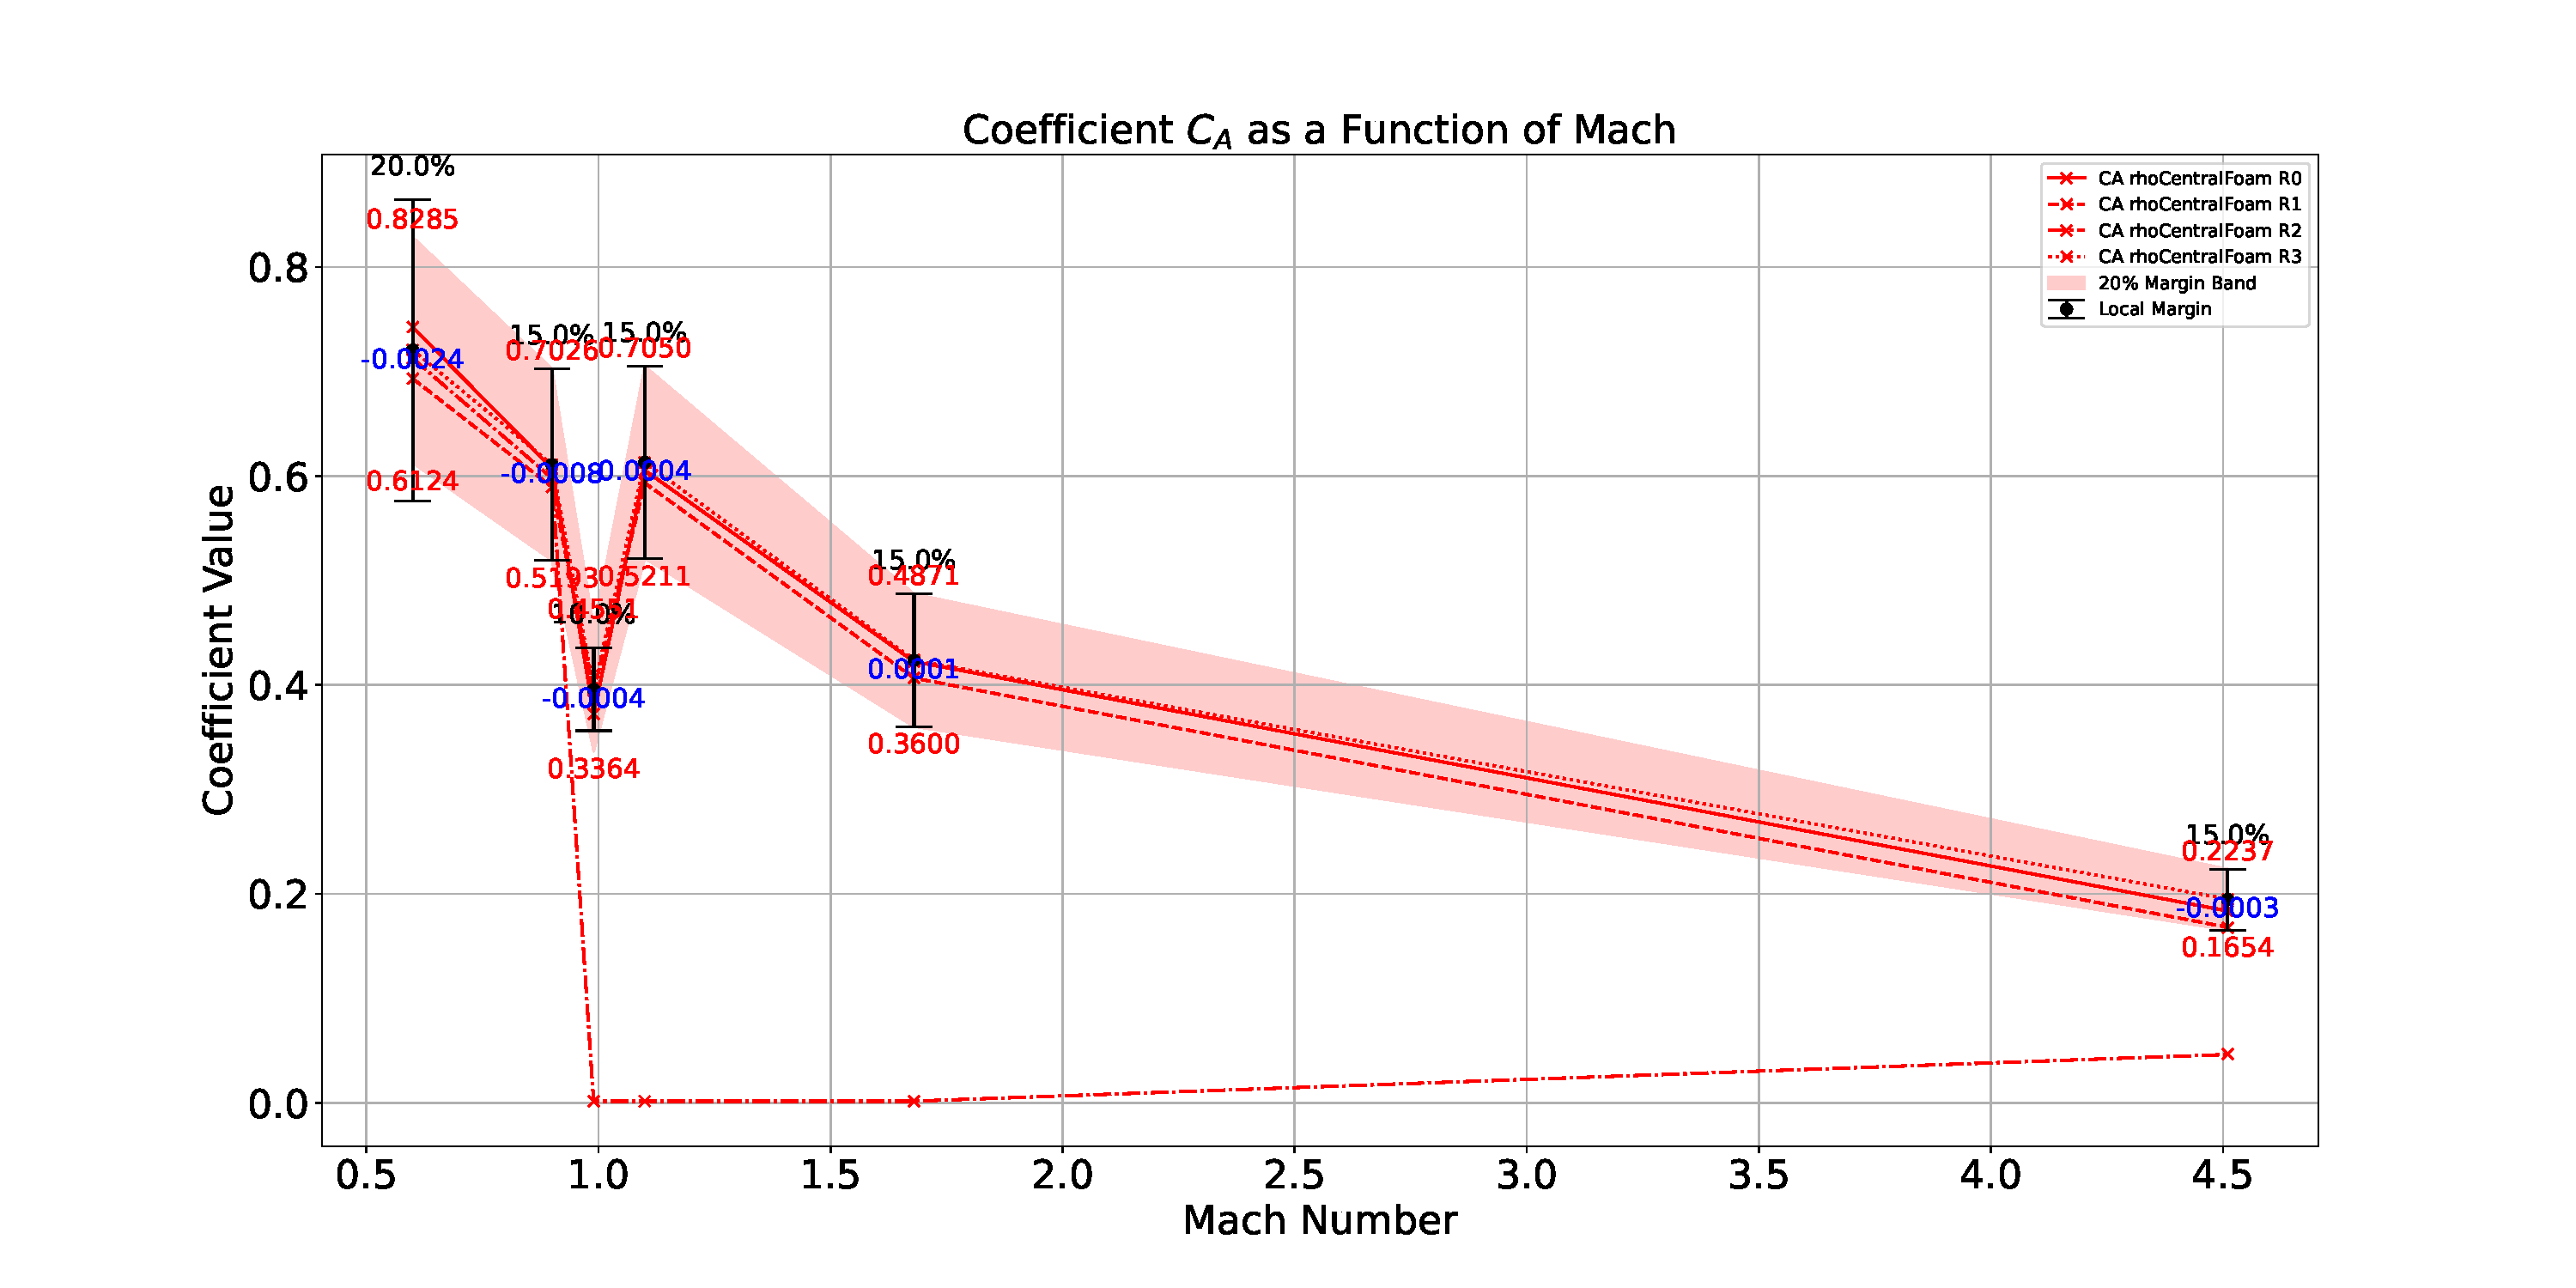
\includegraphics[width=0.995\linewidth]{figs/eris/eris_CA.pdf}\\
%    %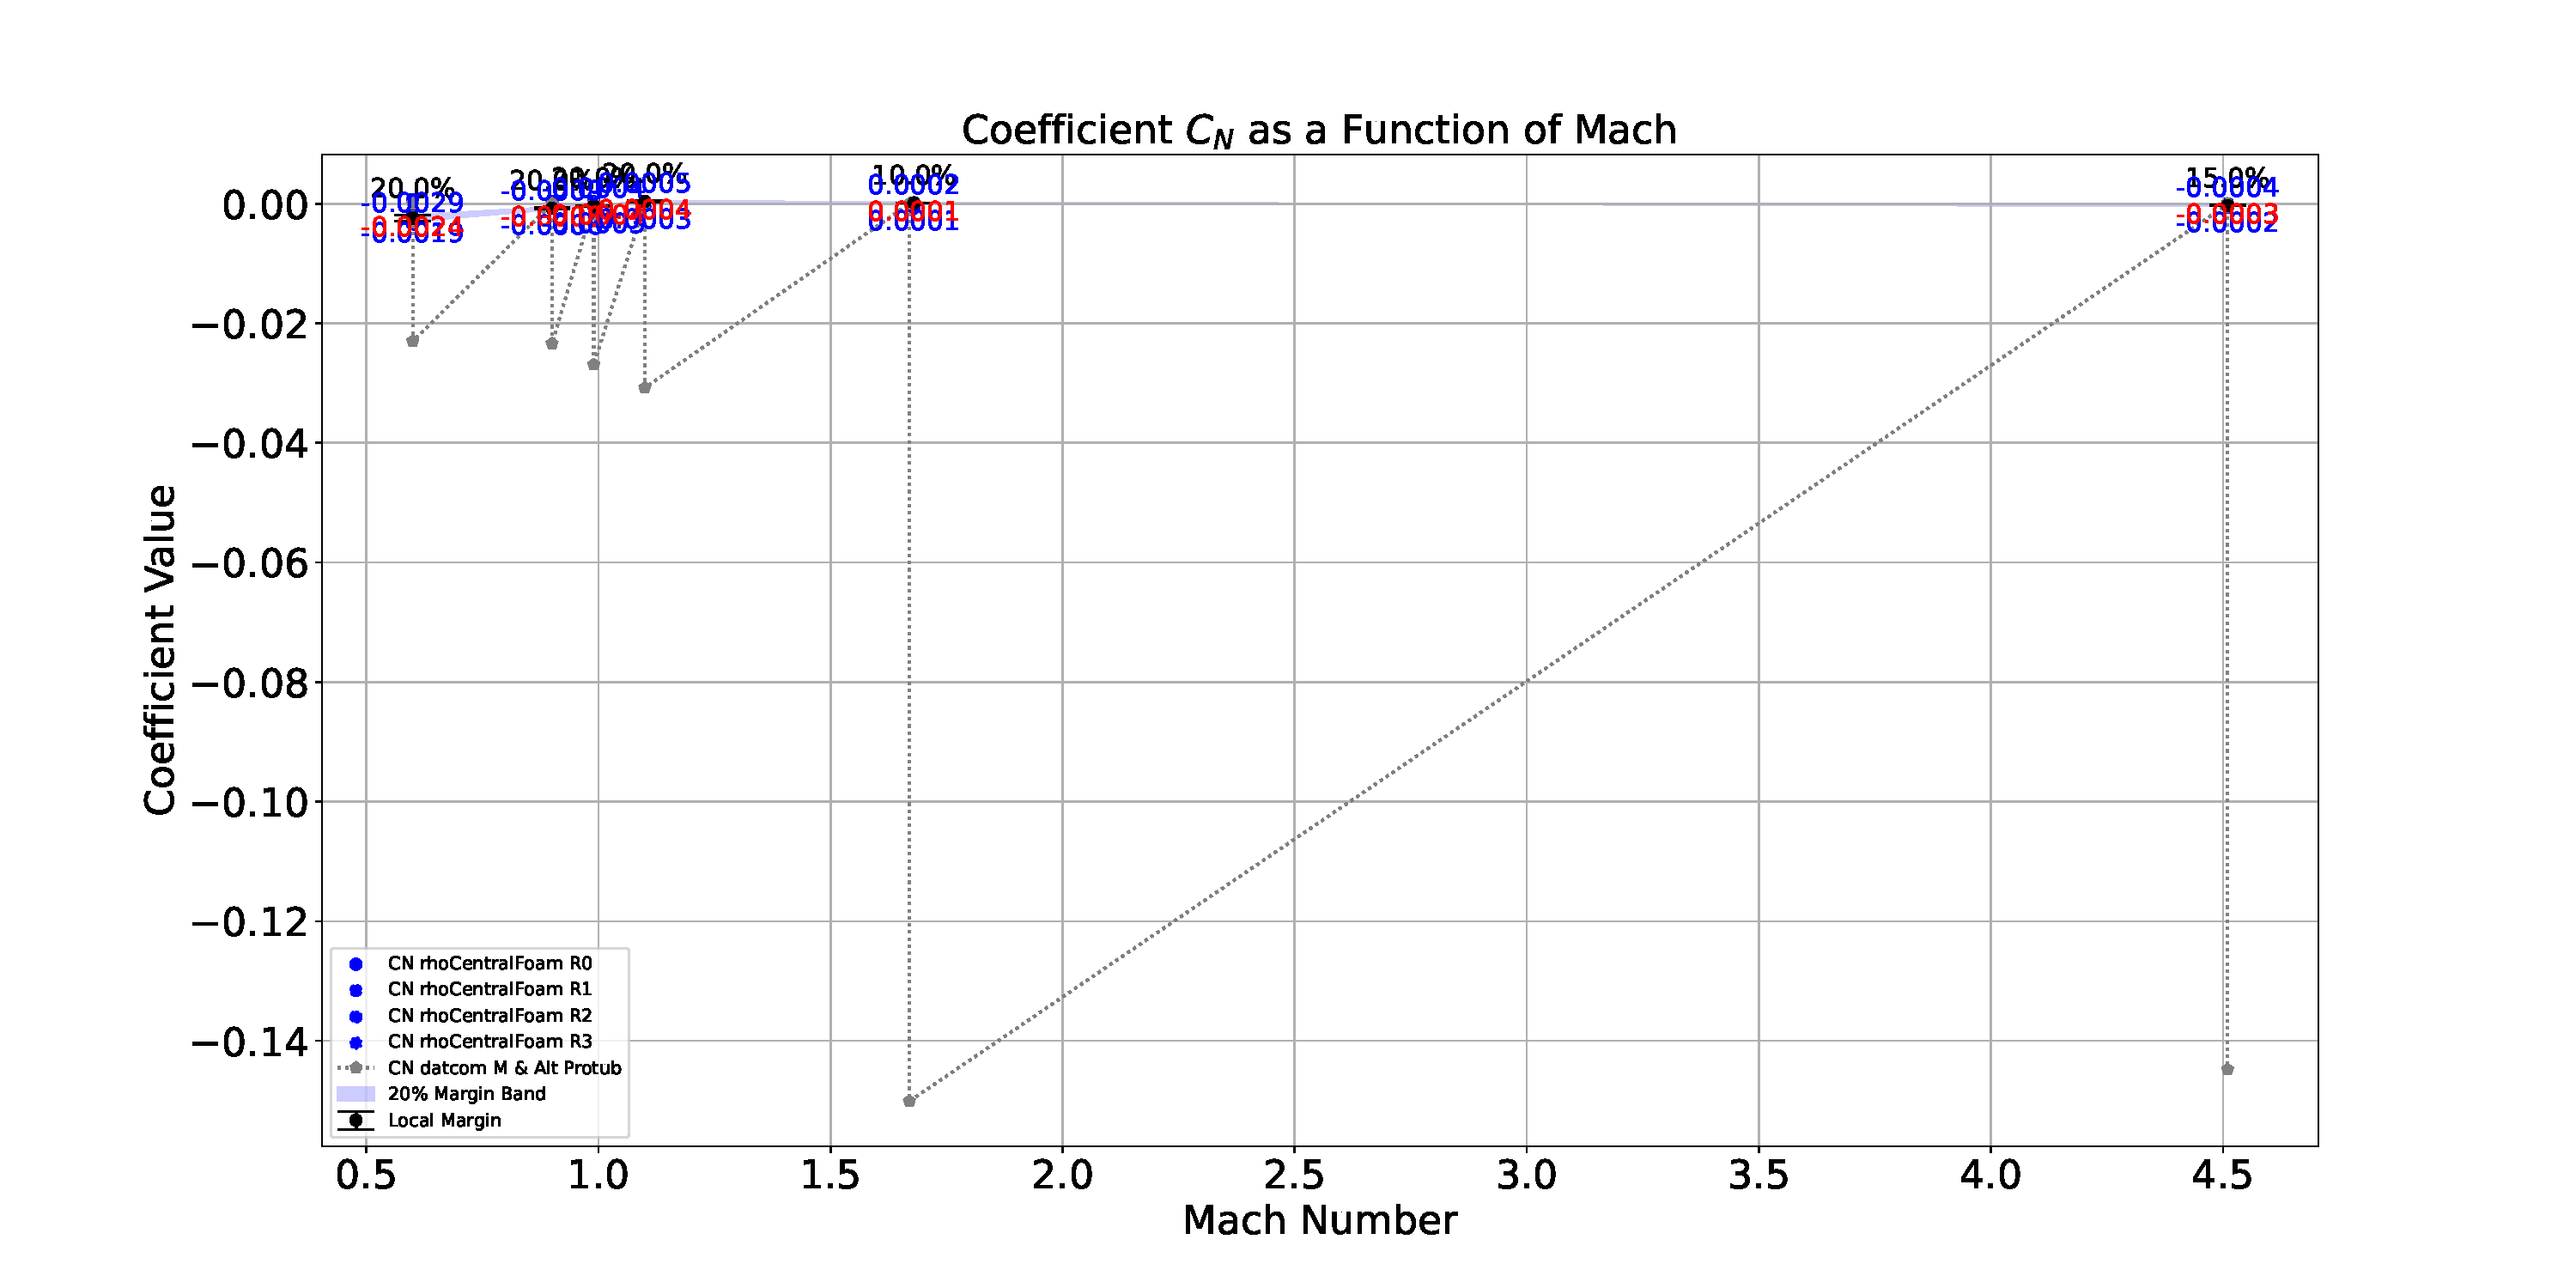
\includegraphics[width=0.995\linewidth]{figs/eris/eris_CN.pdf}\\
%    %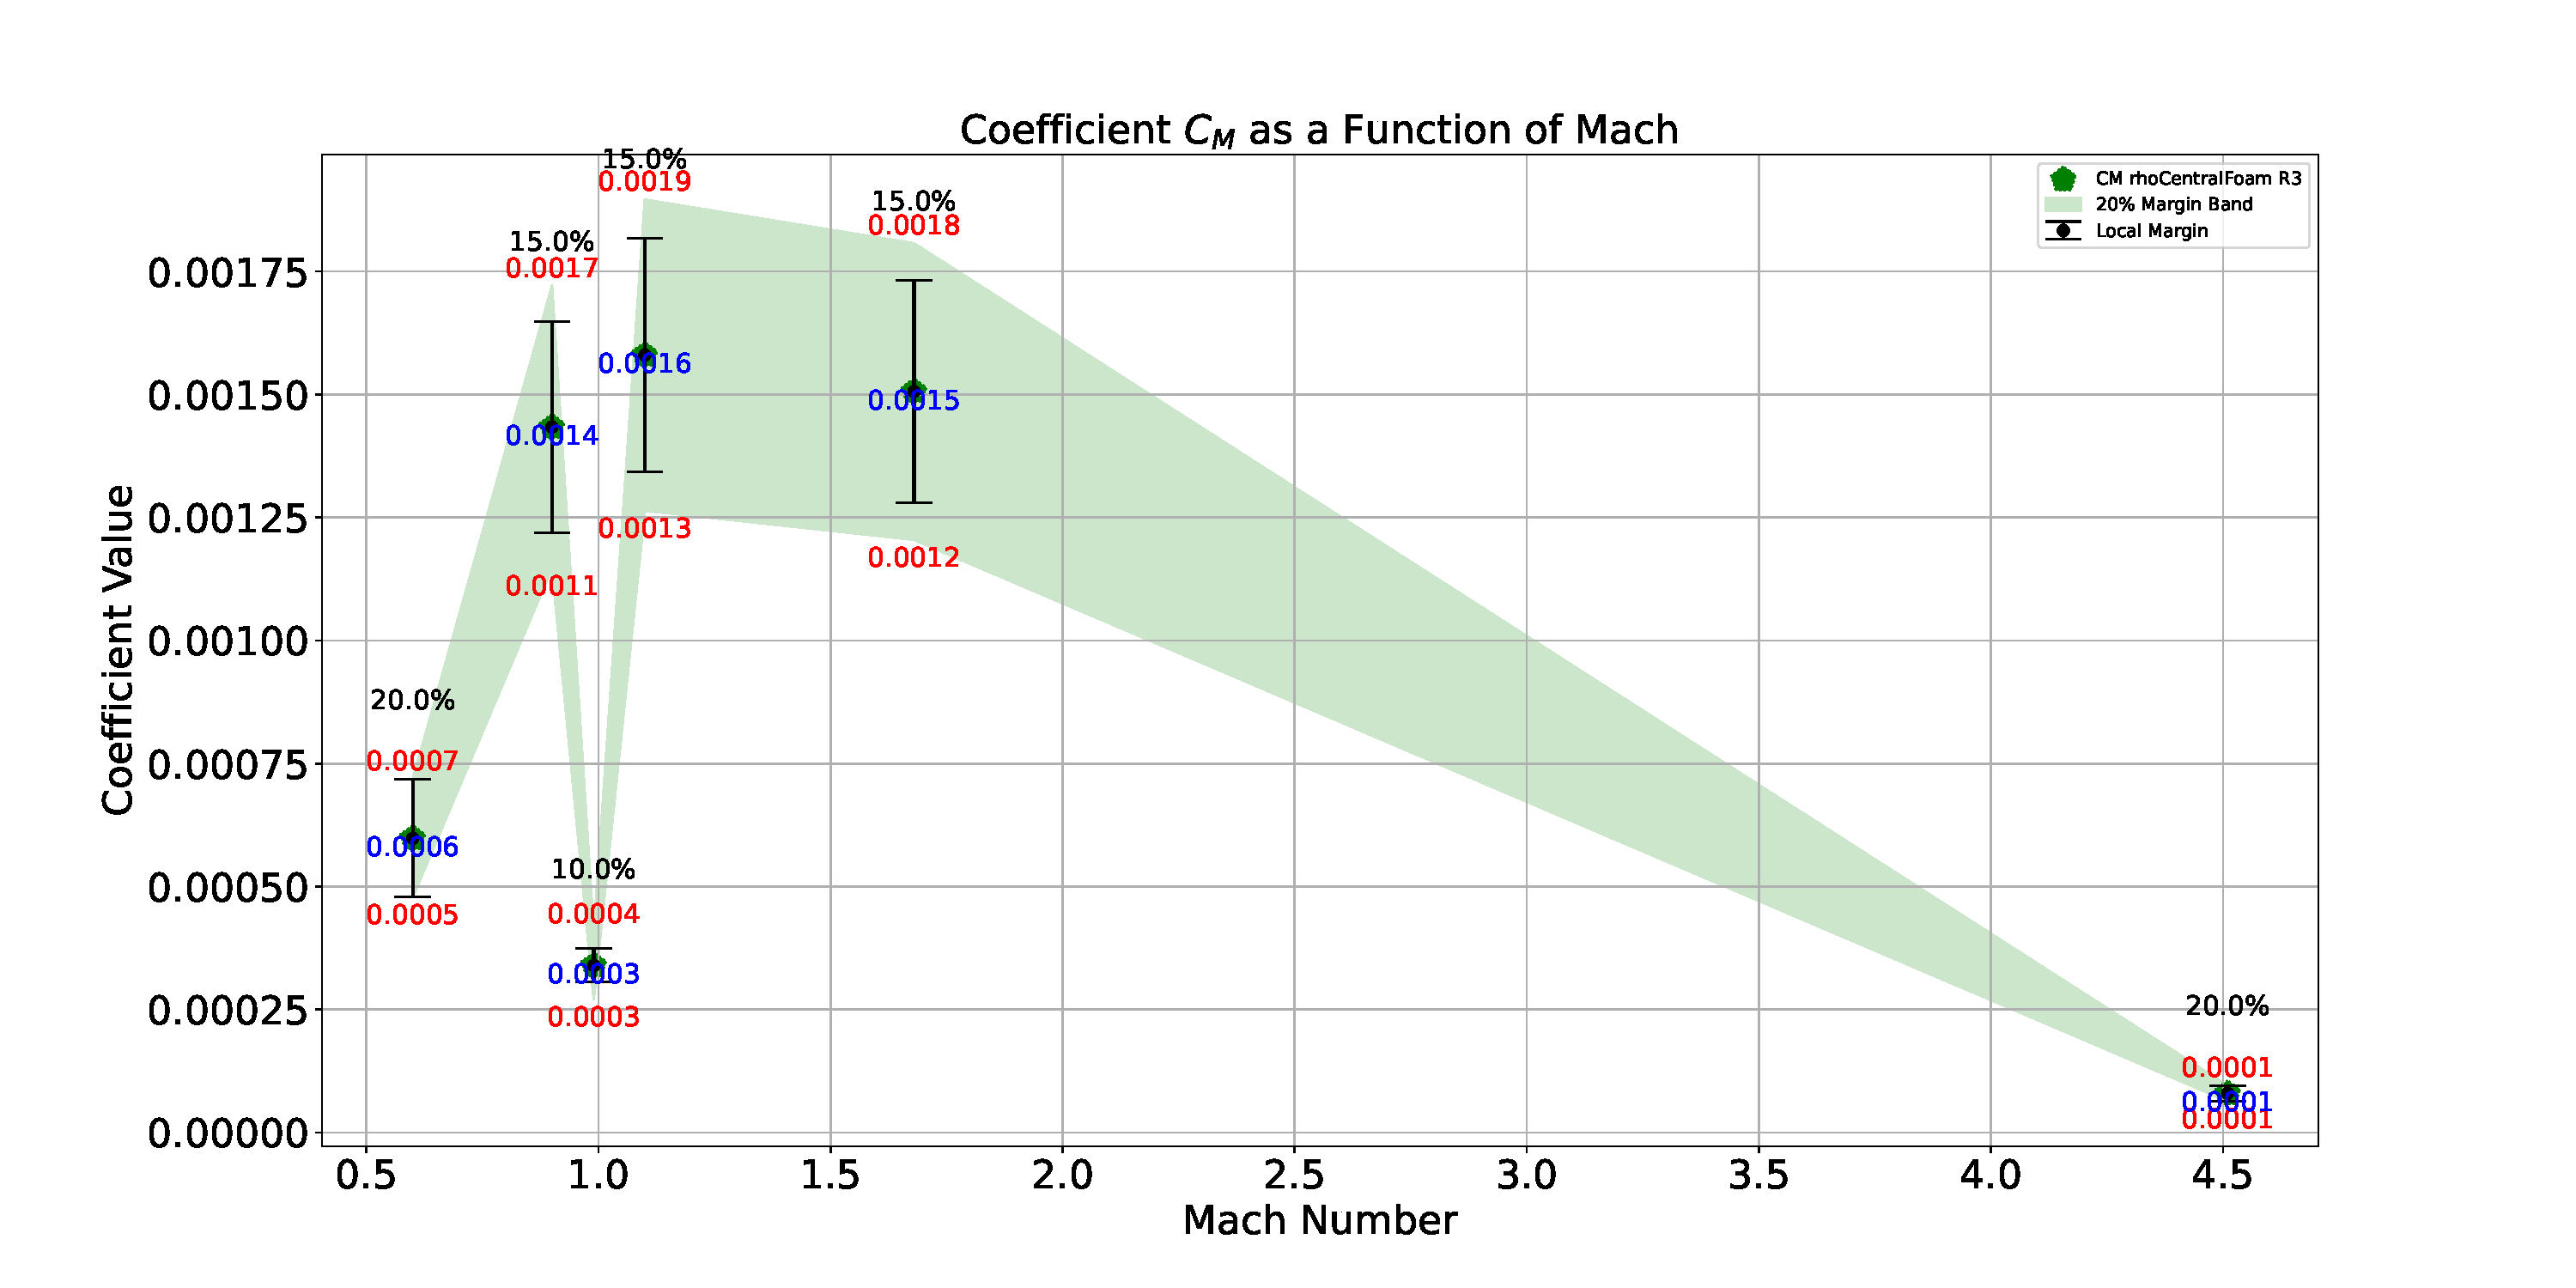
\includegraphics[width=0.995\linewidth]{figs/eris/eris_CM.pdf}
%    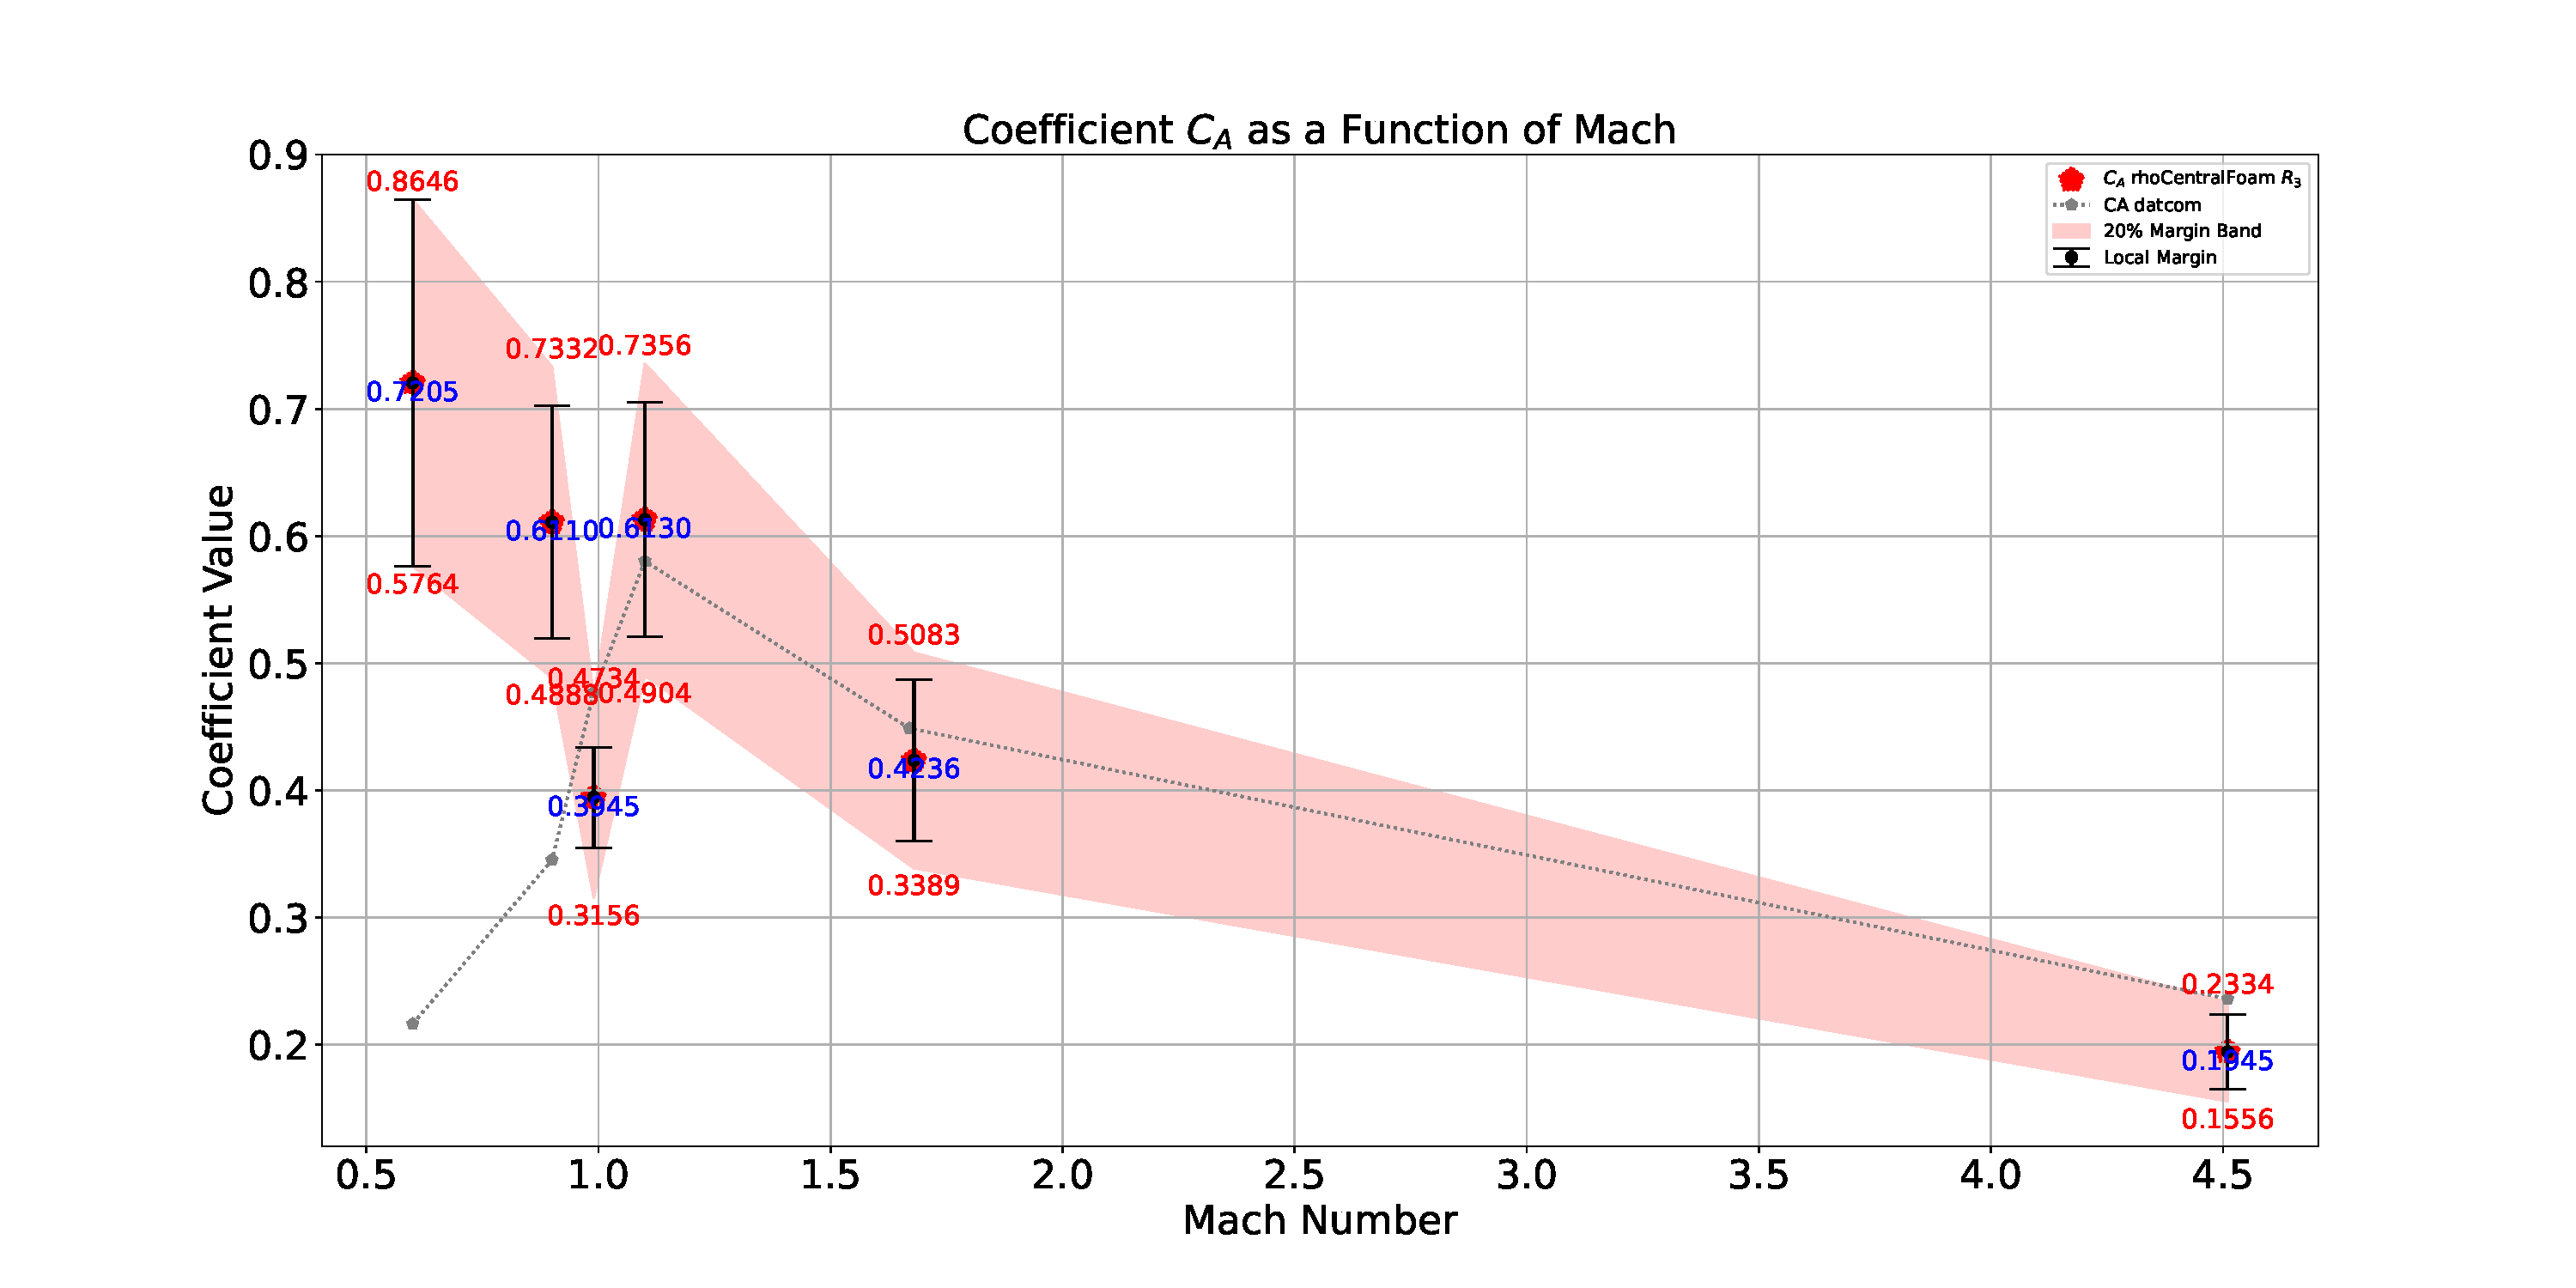
\includegraphics[width=0.995\linewidth]{figs/eris/eris0_CA.pdf}\\
%    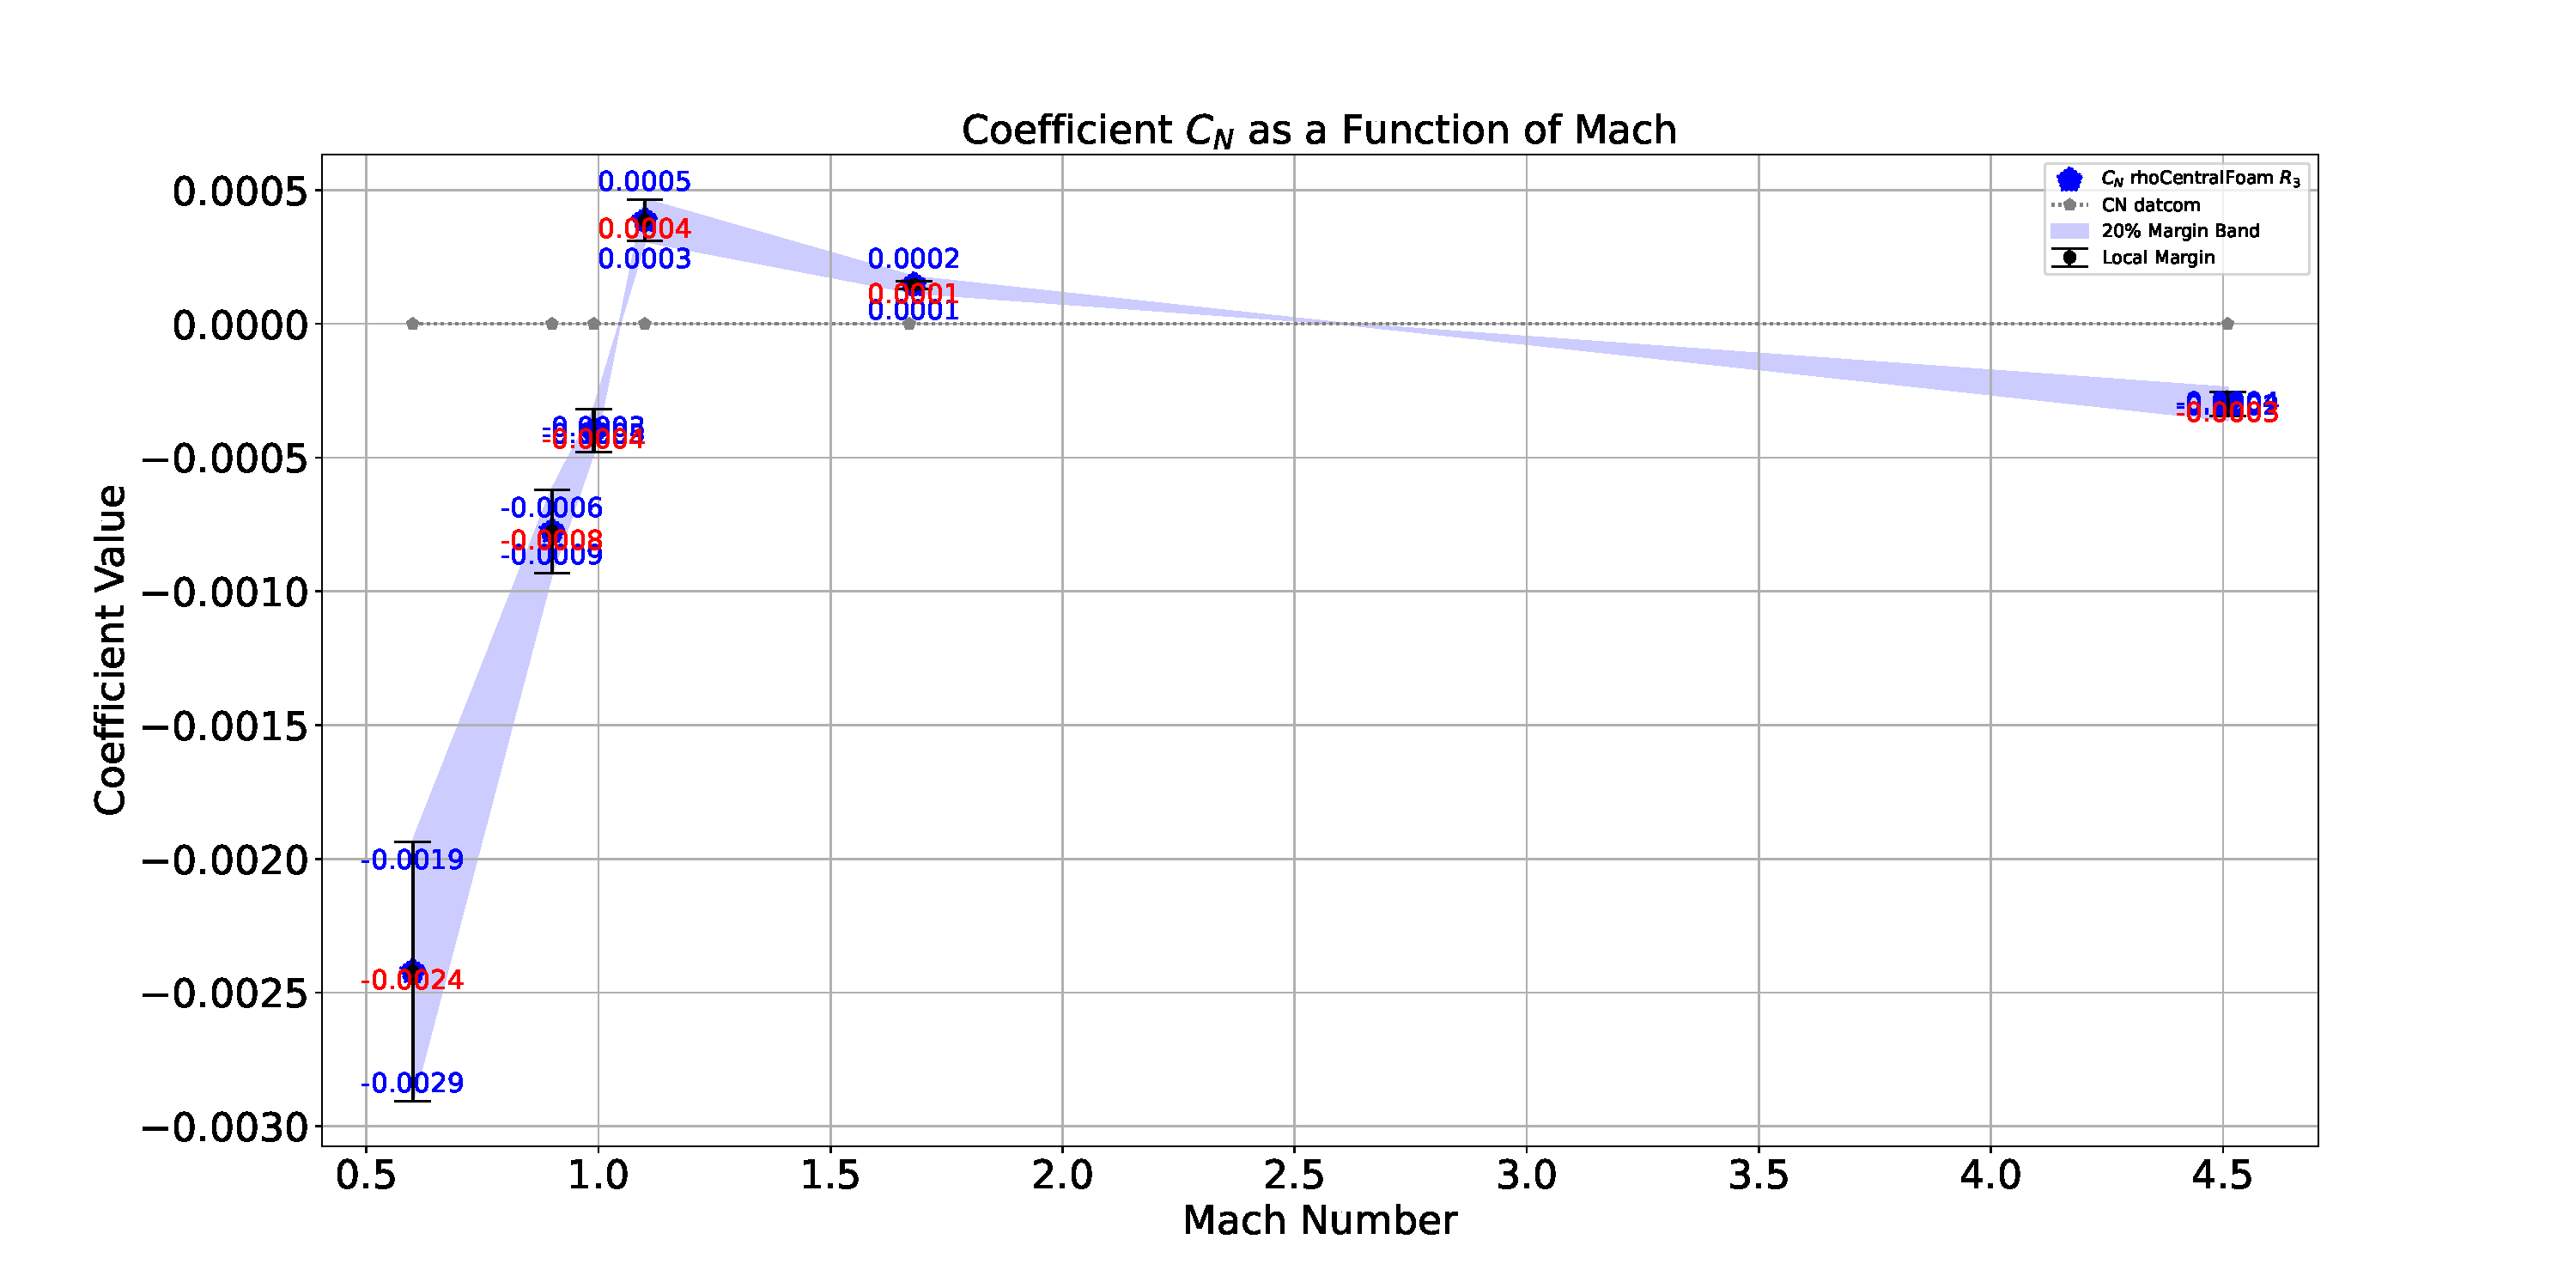
\includegraphics[width=0.995\linewidth]{figs/eris/eris0_CN.pdf}\\
%    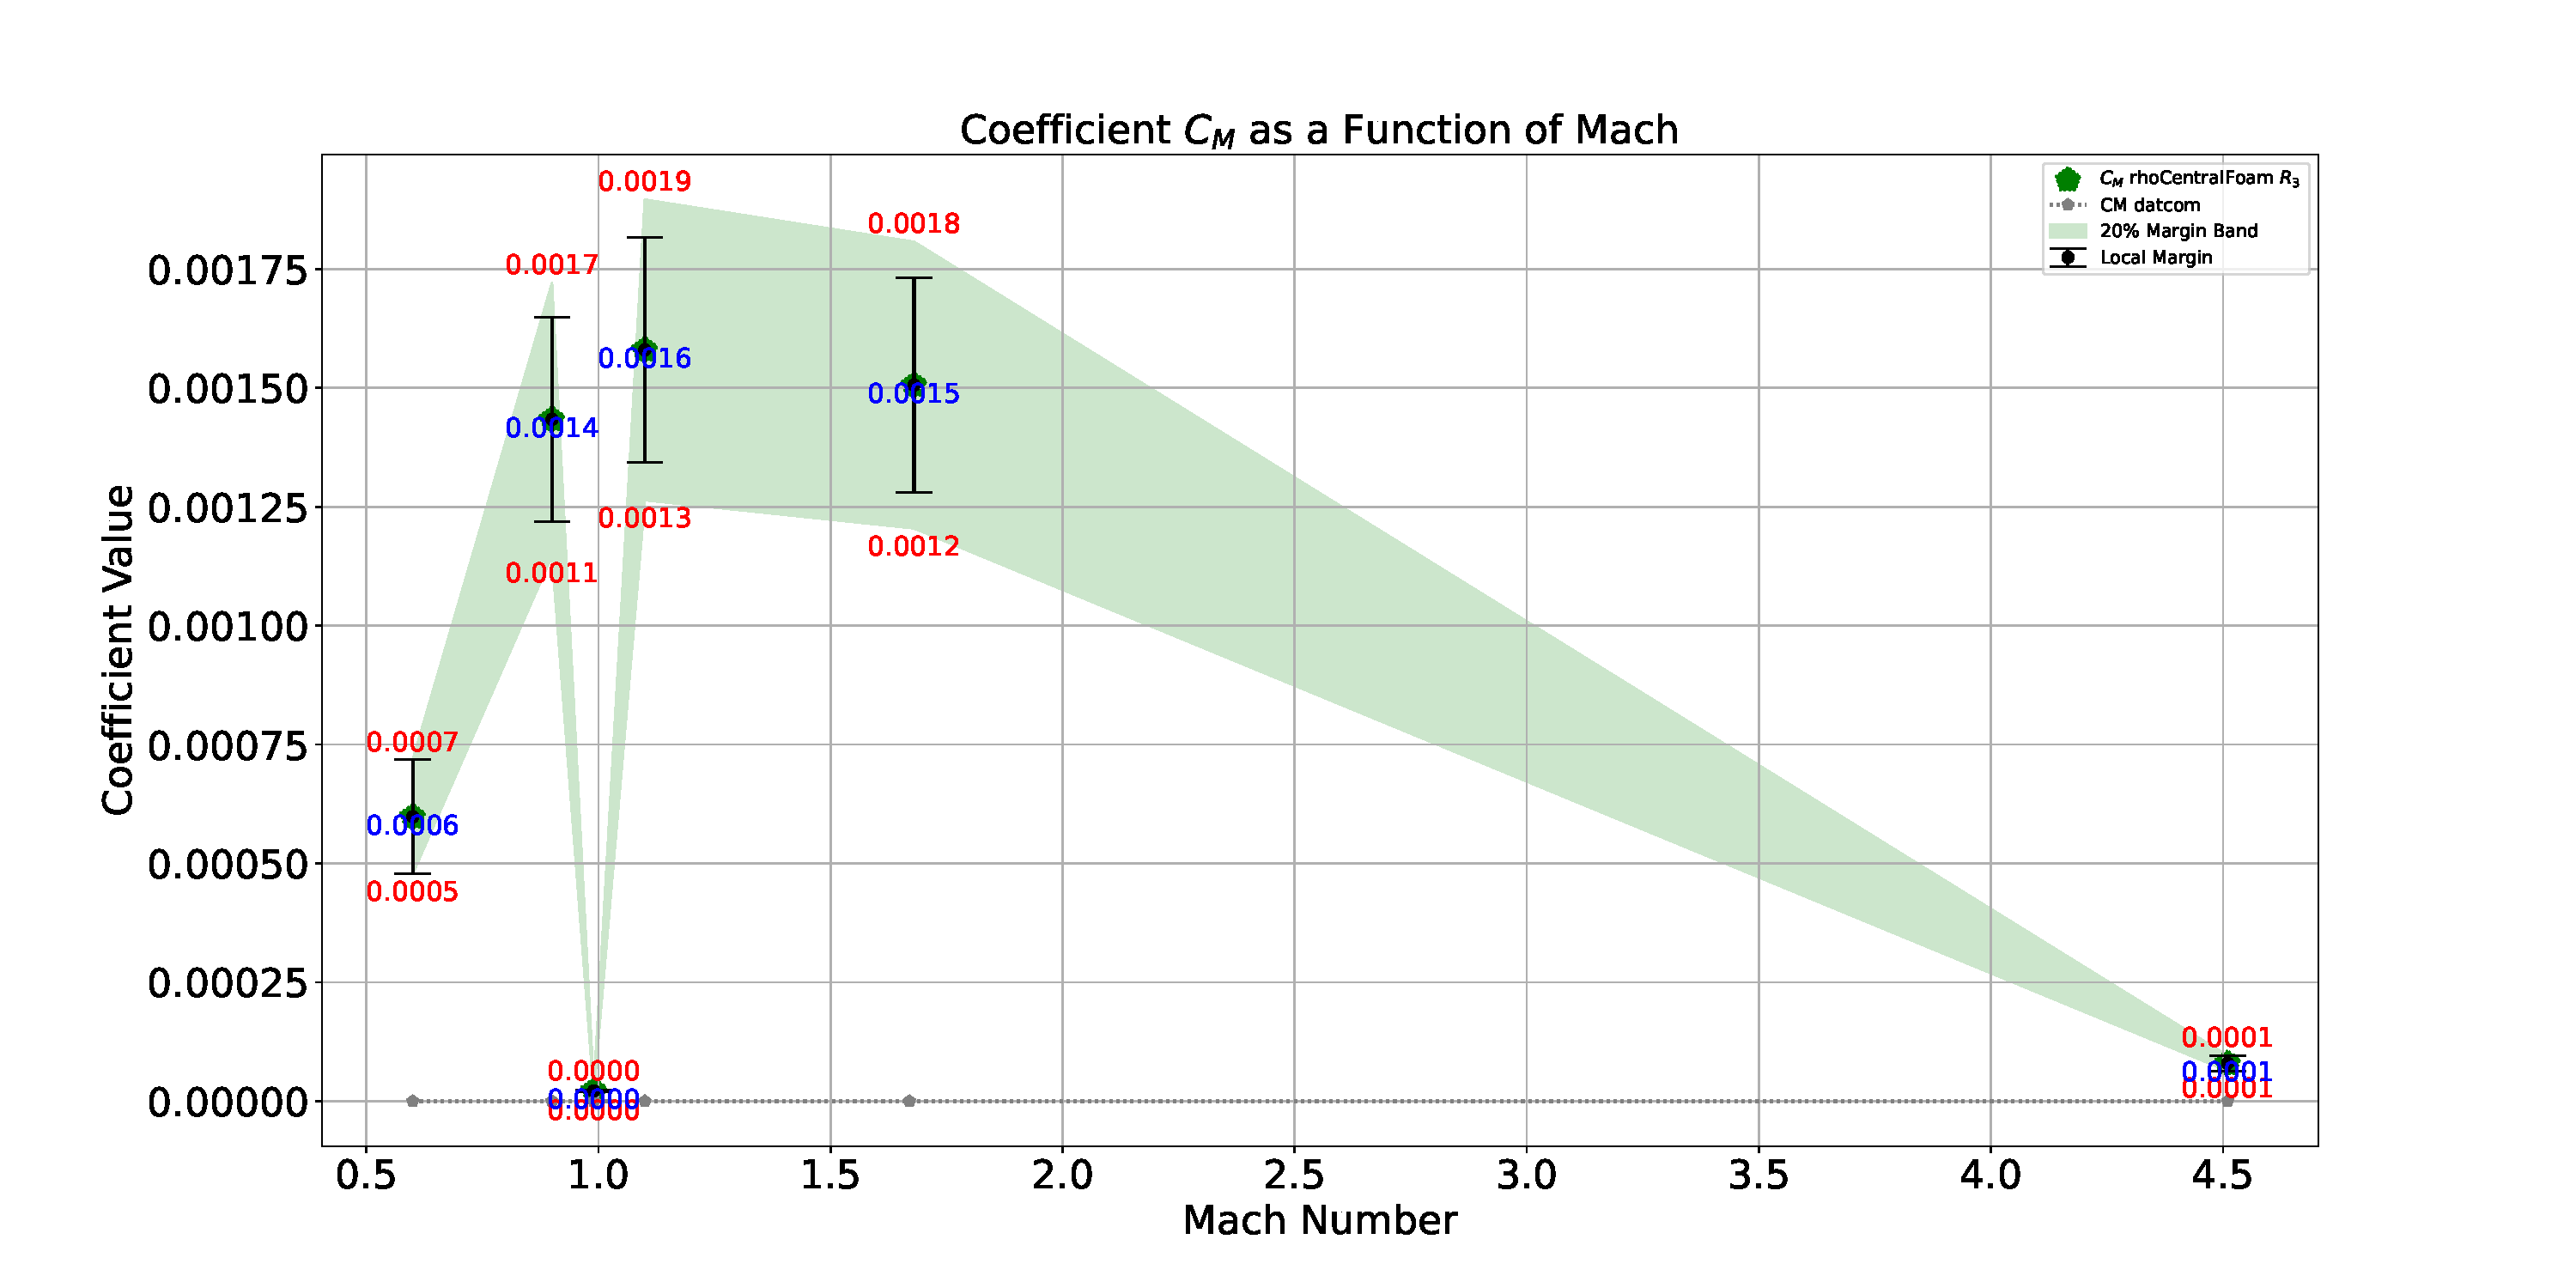
\includegraphics[width=0.995\linewidth]{figs/eris/eris0_CM.pdf}
%    %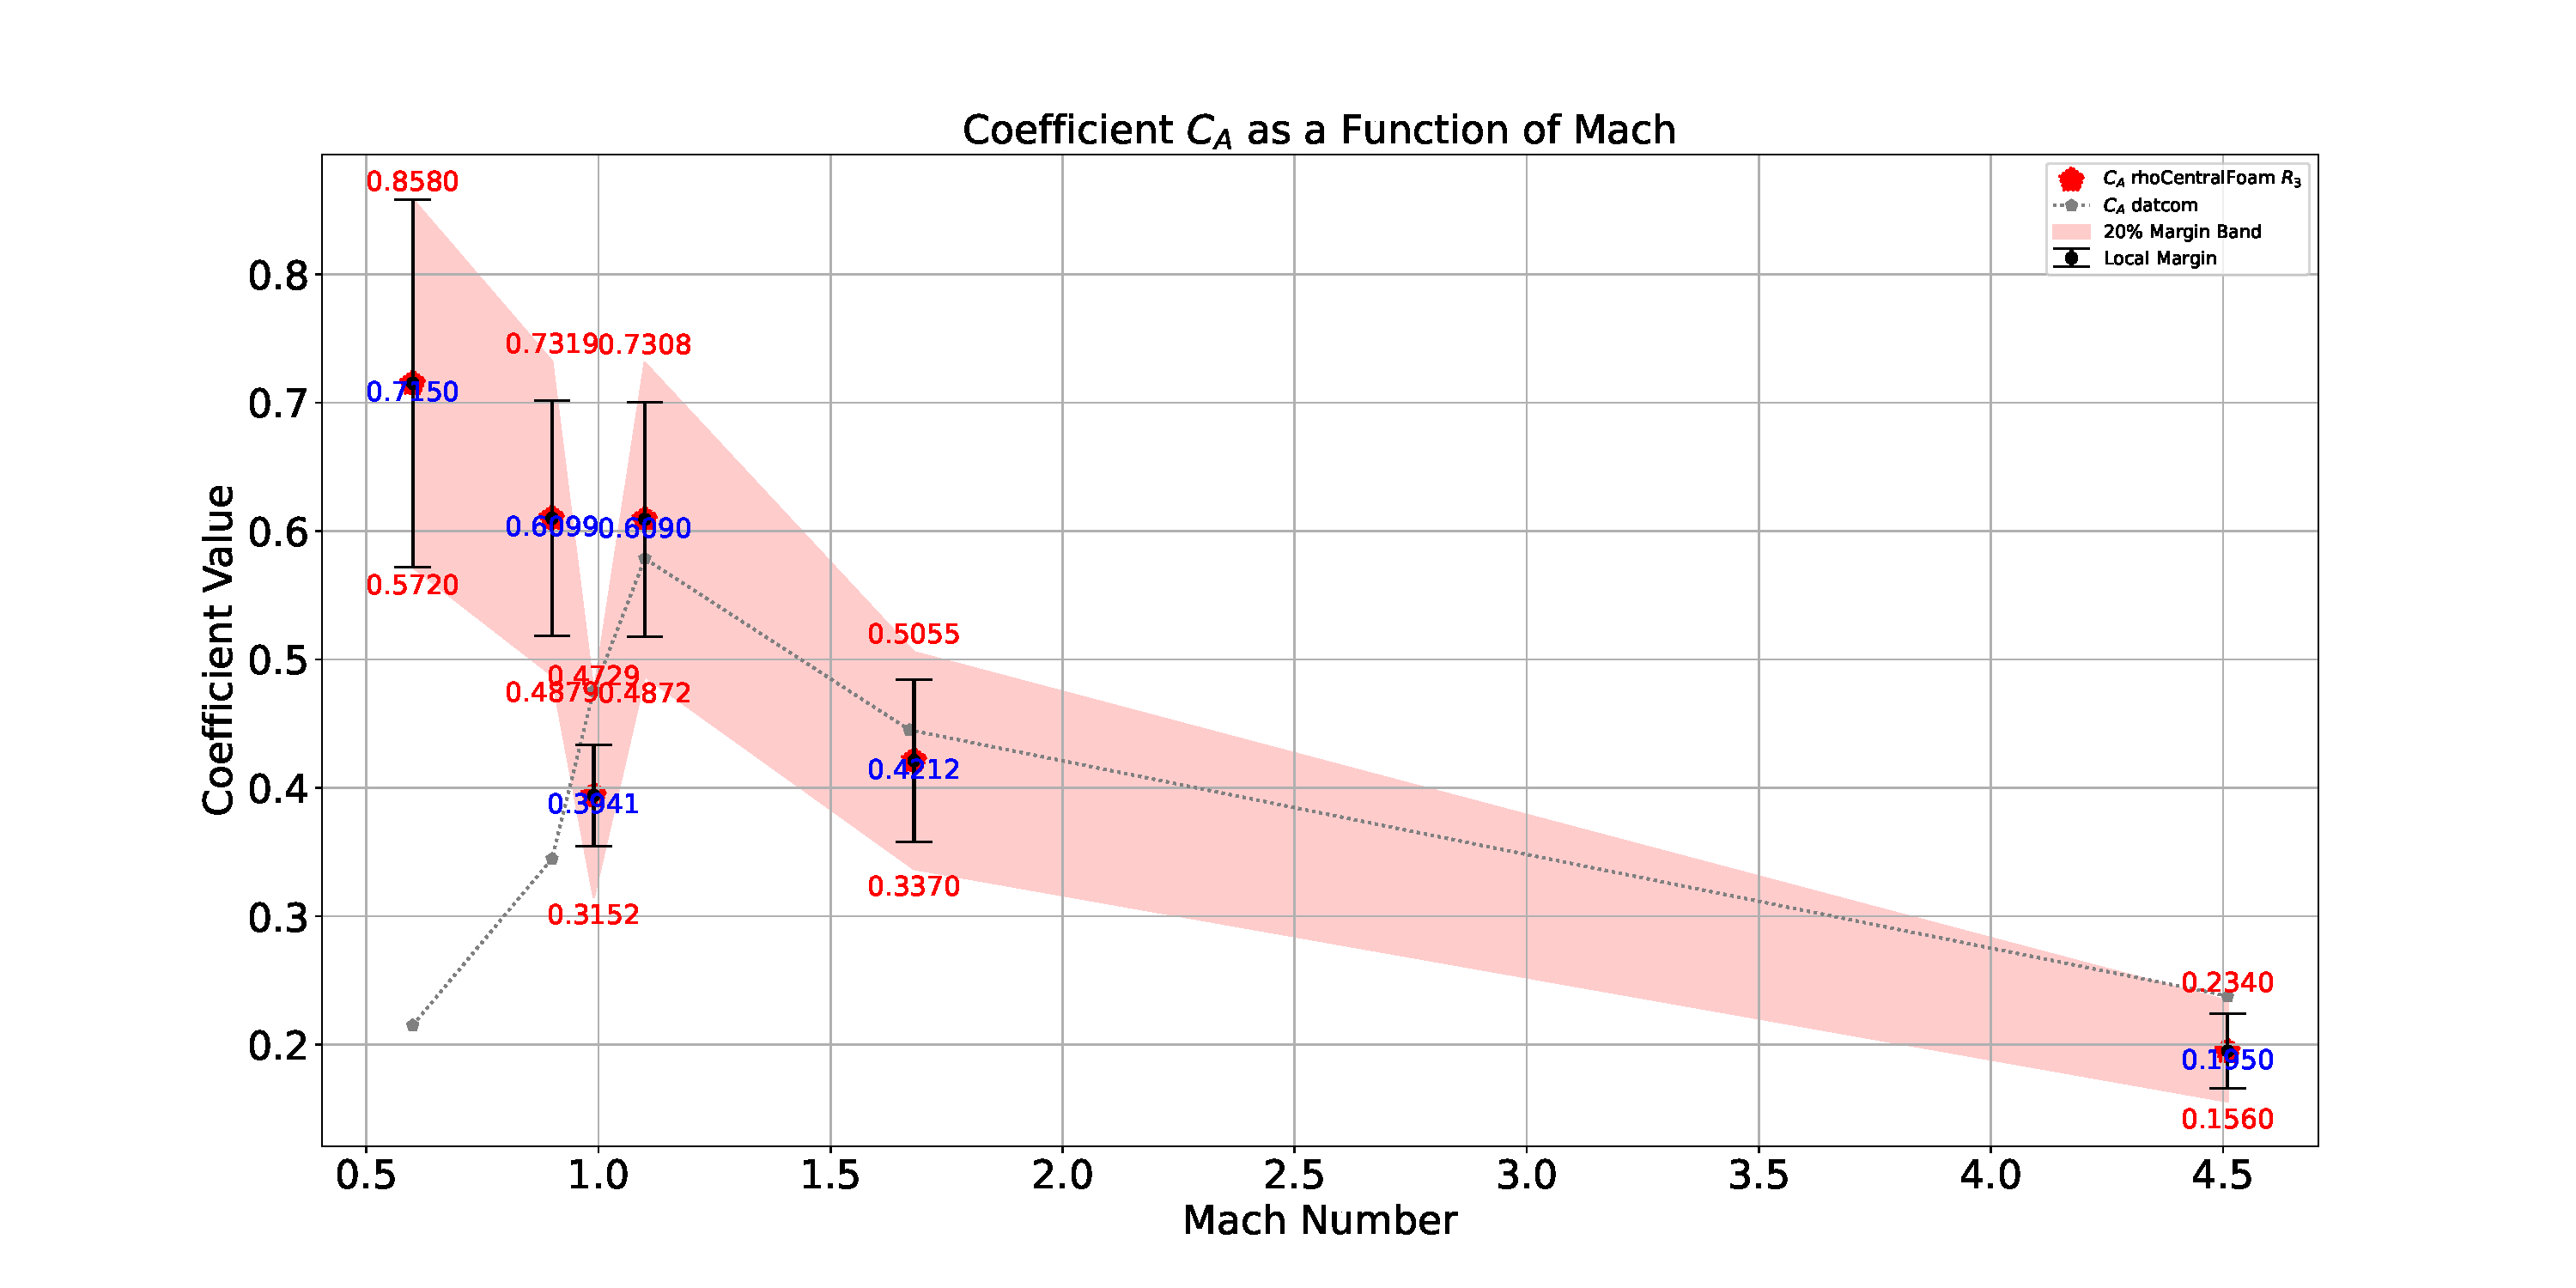
\includegraphics[width=0.995\linewidth]{figs/eris/eris4_CA.pdf}\\
%    %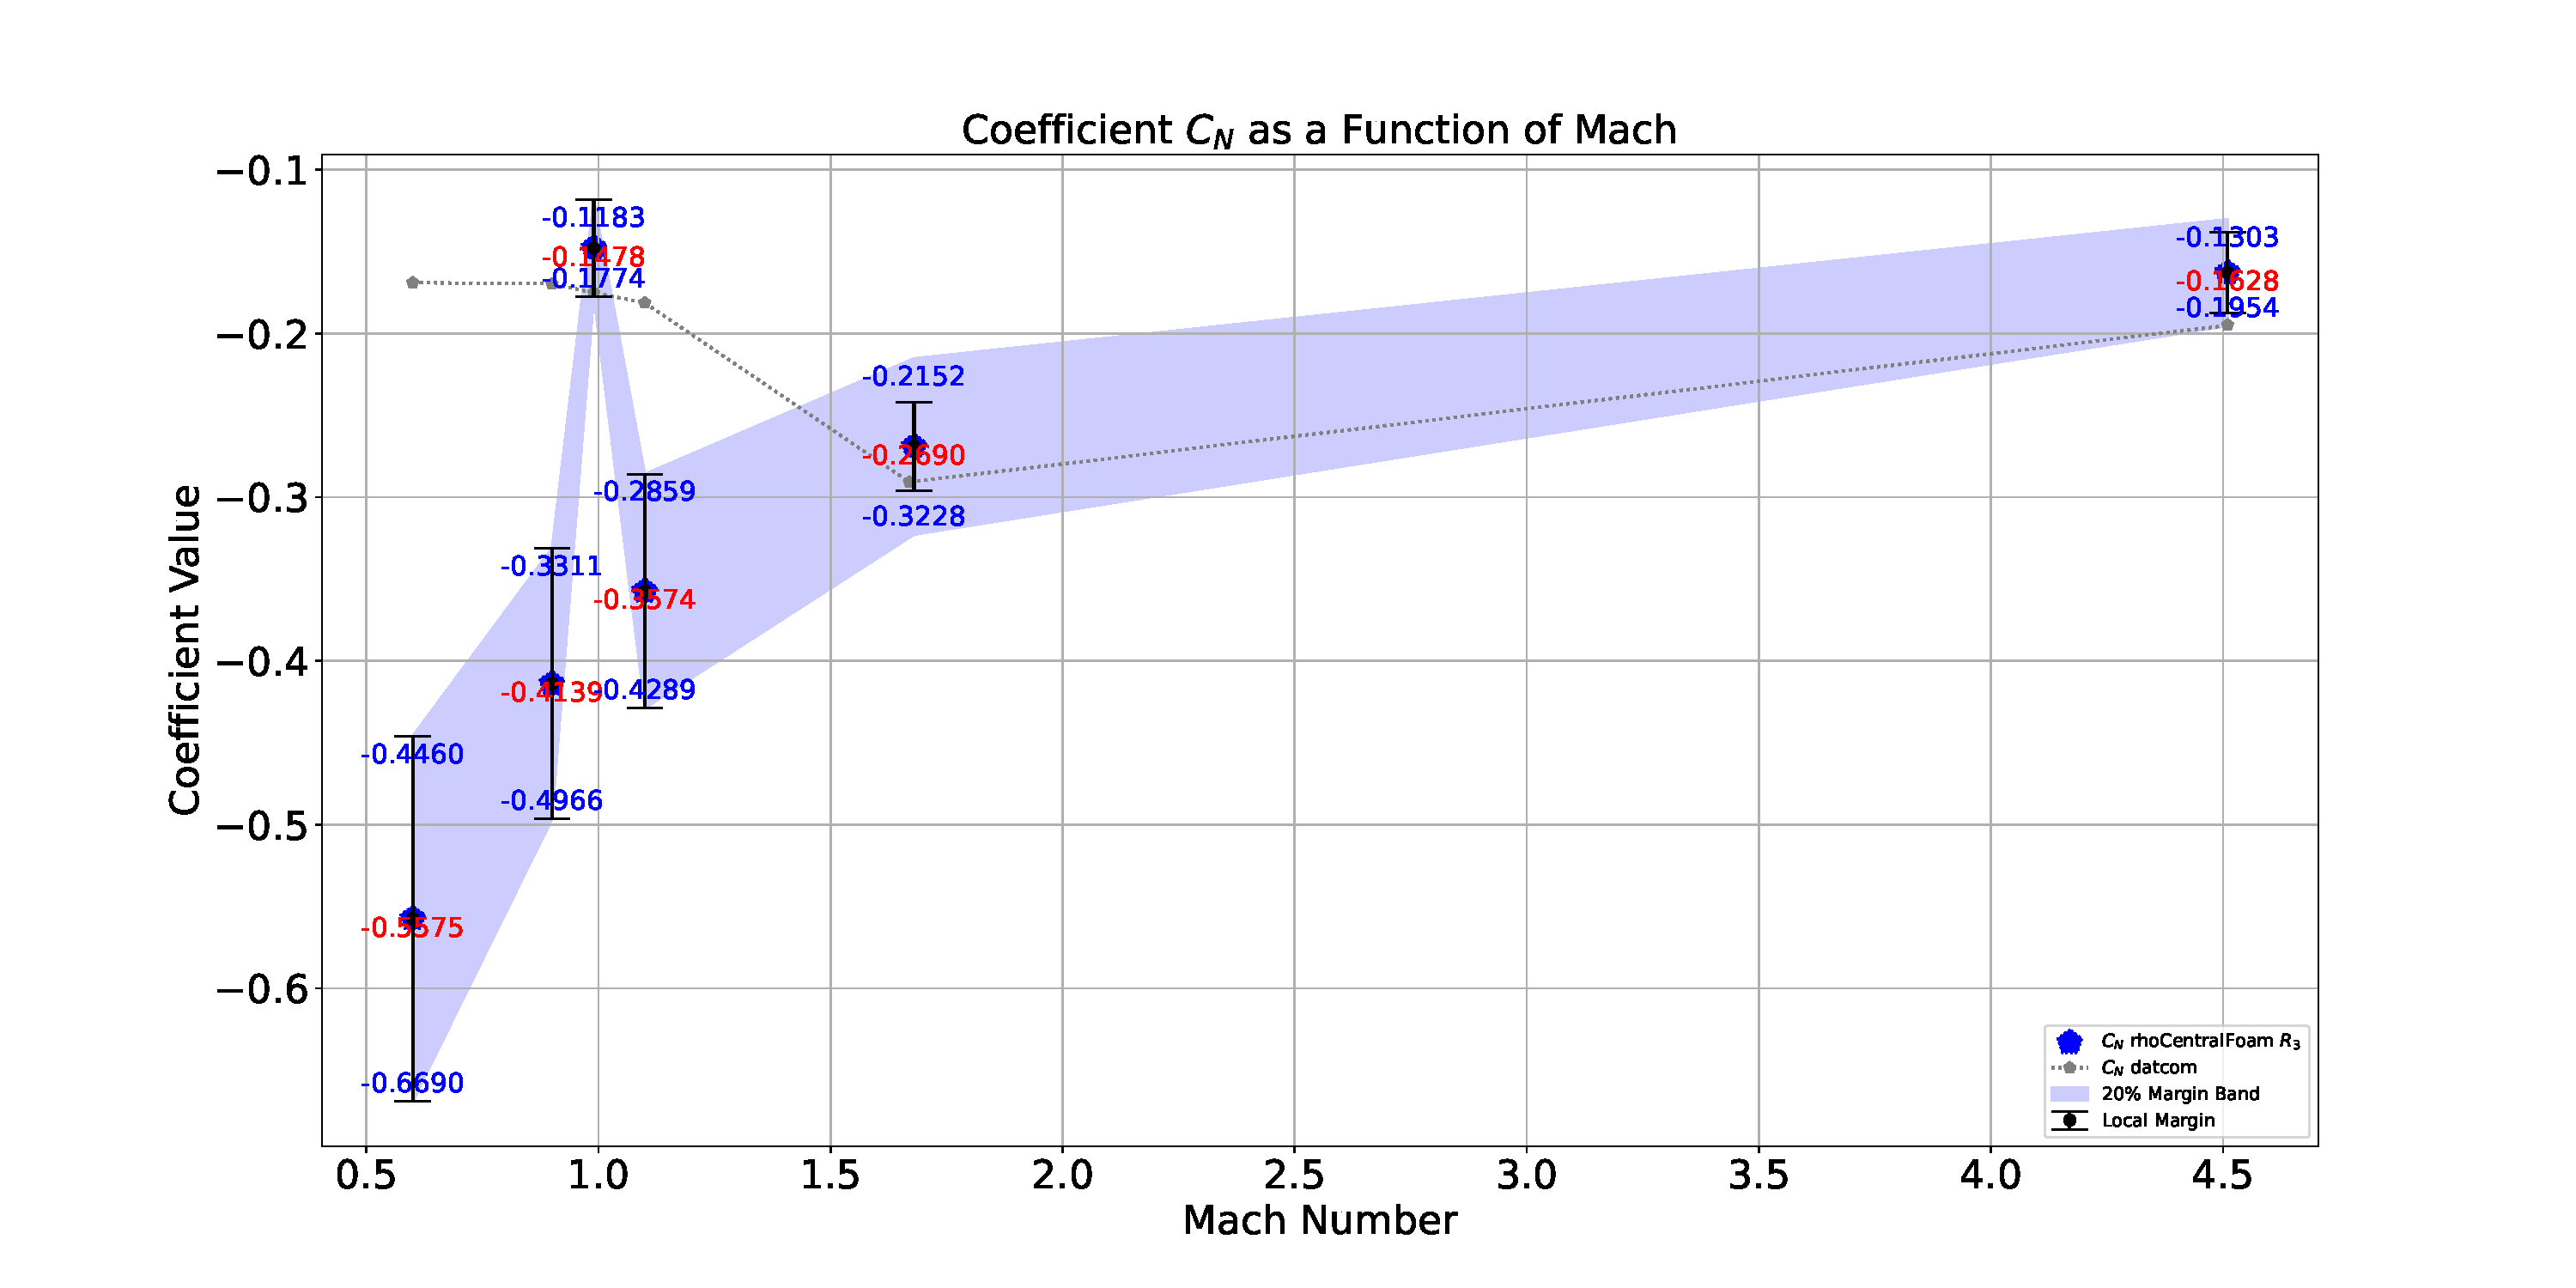
\includegraphics[width=0.995\linewidth]{figs/eris/eris4_CN.pdf}\\
%    %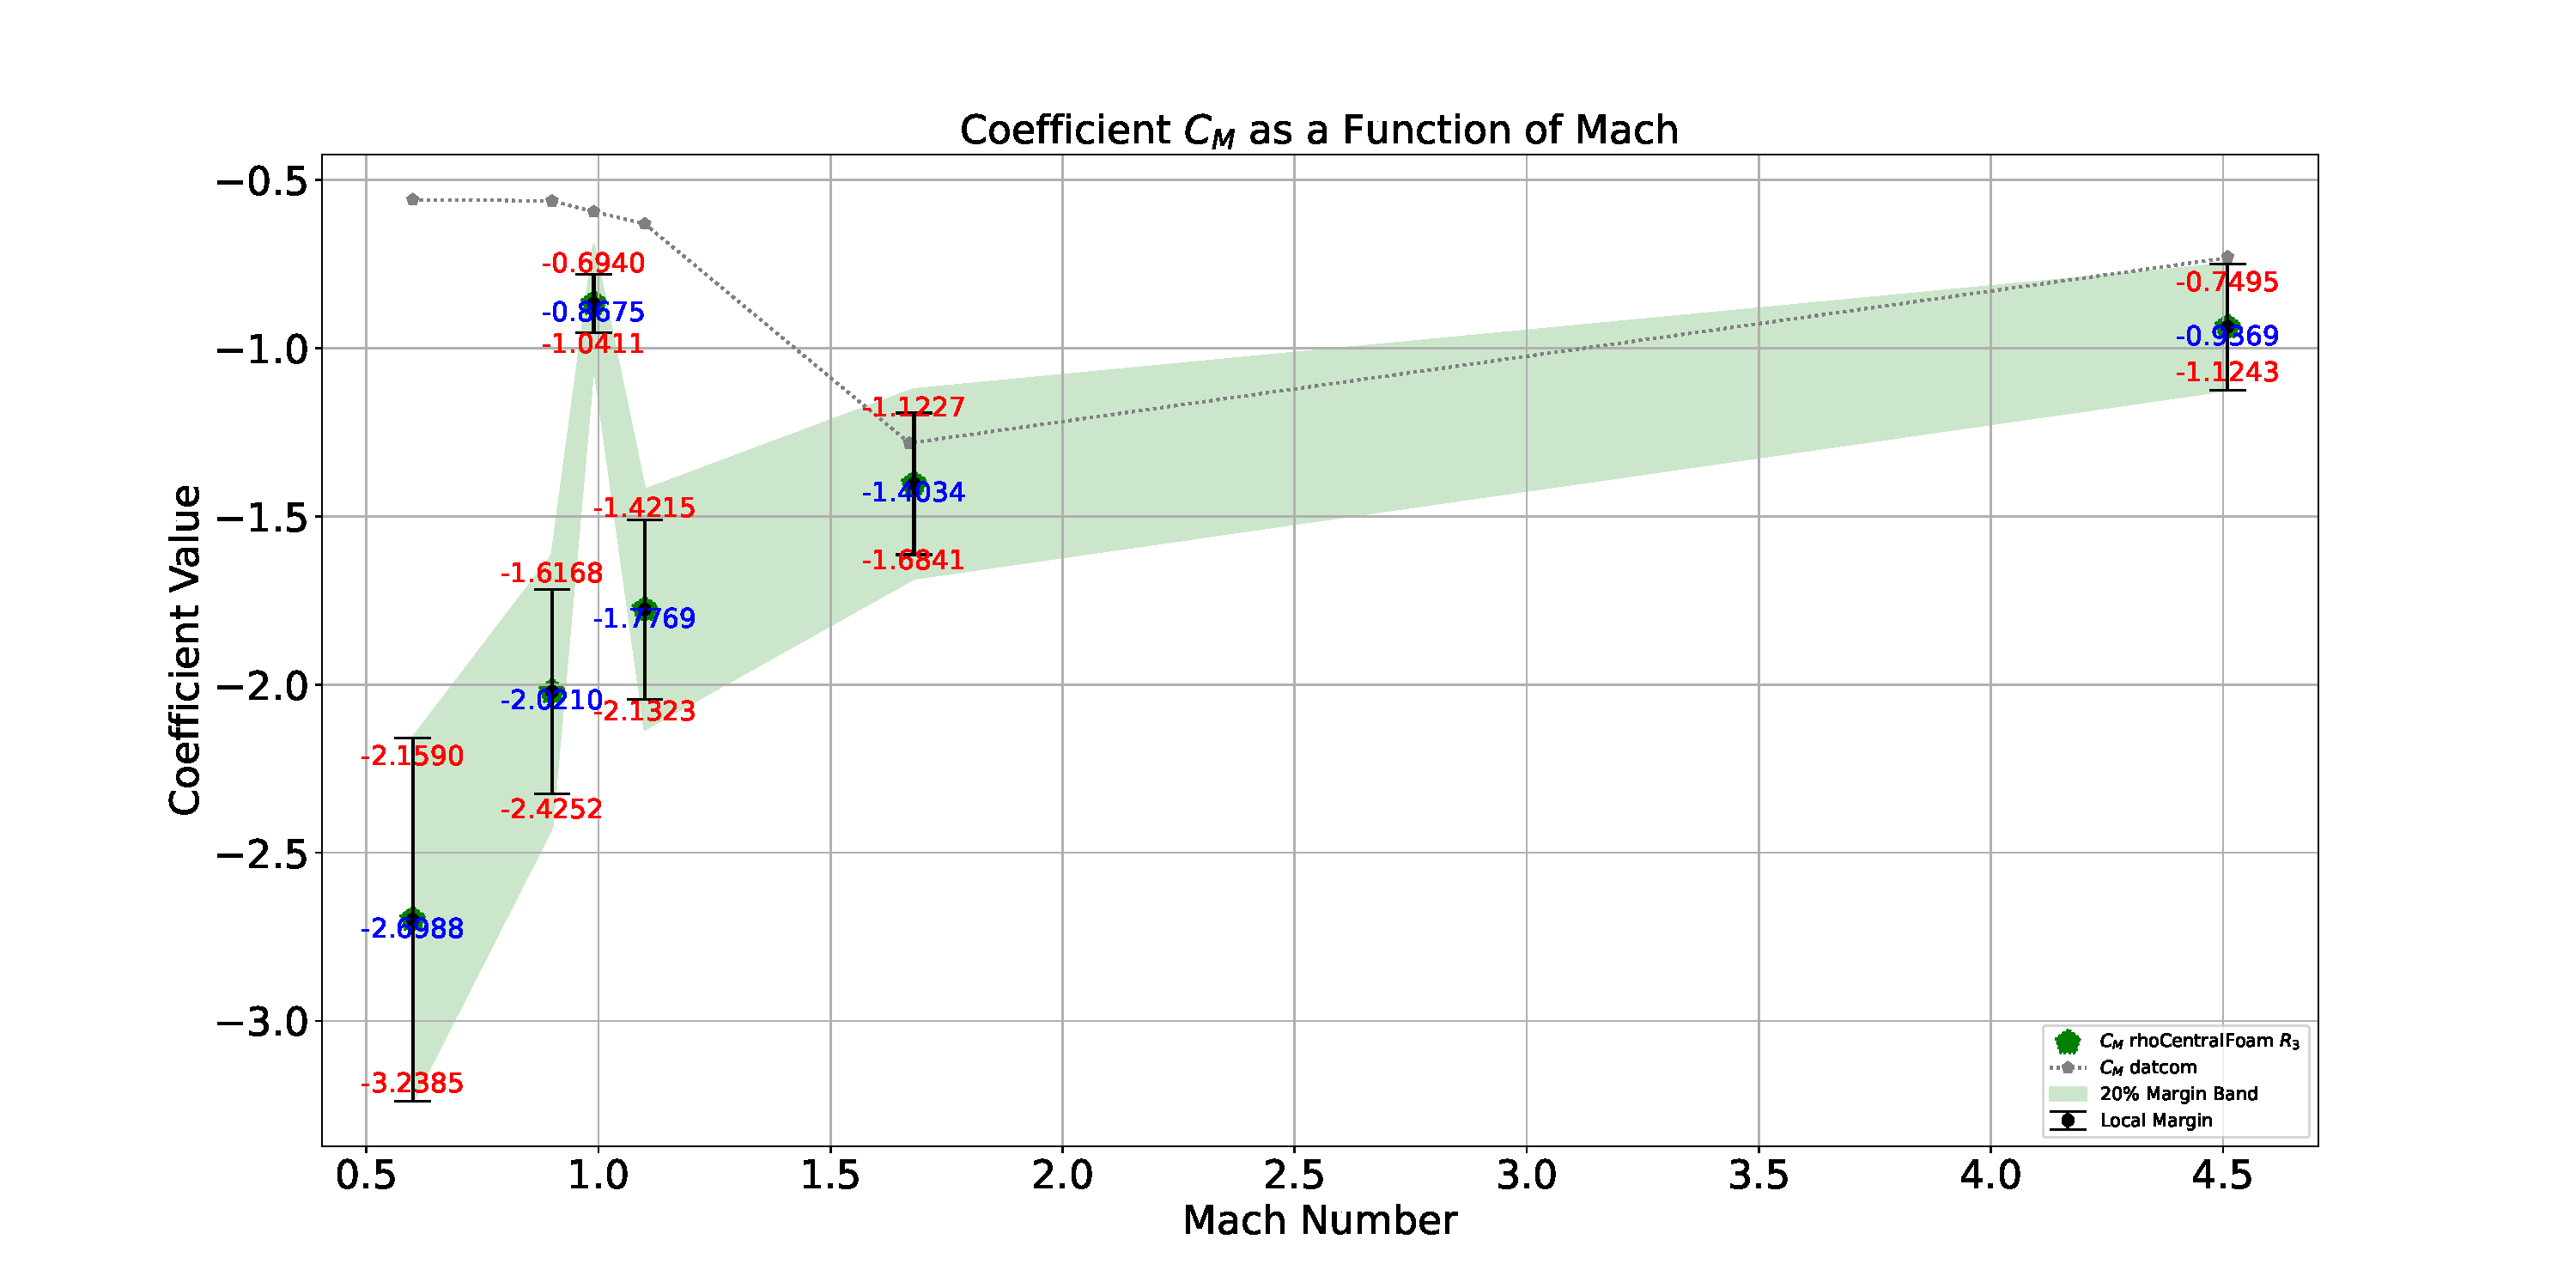
\includegraphics[width=0.995\linewidth]{figs/eris/eris4_CM.pdf}
%    \caption{Aerodynamic coefficients, $C_A$, $C_N$, $C_M$, for the Eris Block 1.1 Rev. A configuration \textbf{S123F} launch vehicle as a function of Mach number for an angle of attach $\alpha$ = 0$^\circ$. The applied uncertainty margin was imported from the benchmark validation test case ARCAS.}
%    \label{fig:eris-CA-CA-CM_alpha0}
%\end{figure}
%
\begin{figure}[H]
    \centering
    \vspace{-0.4cm}
    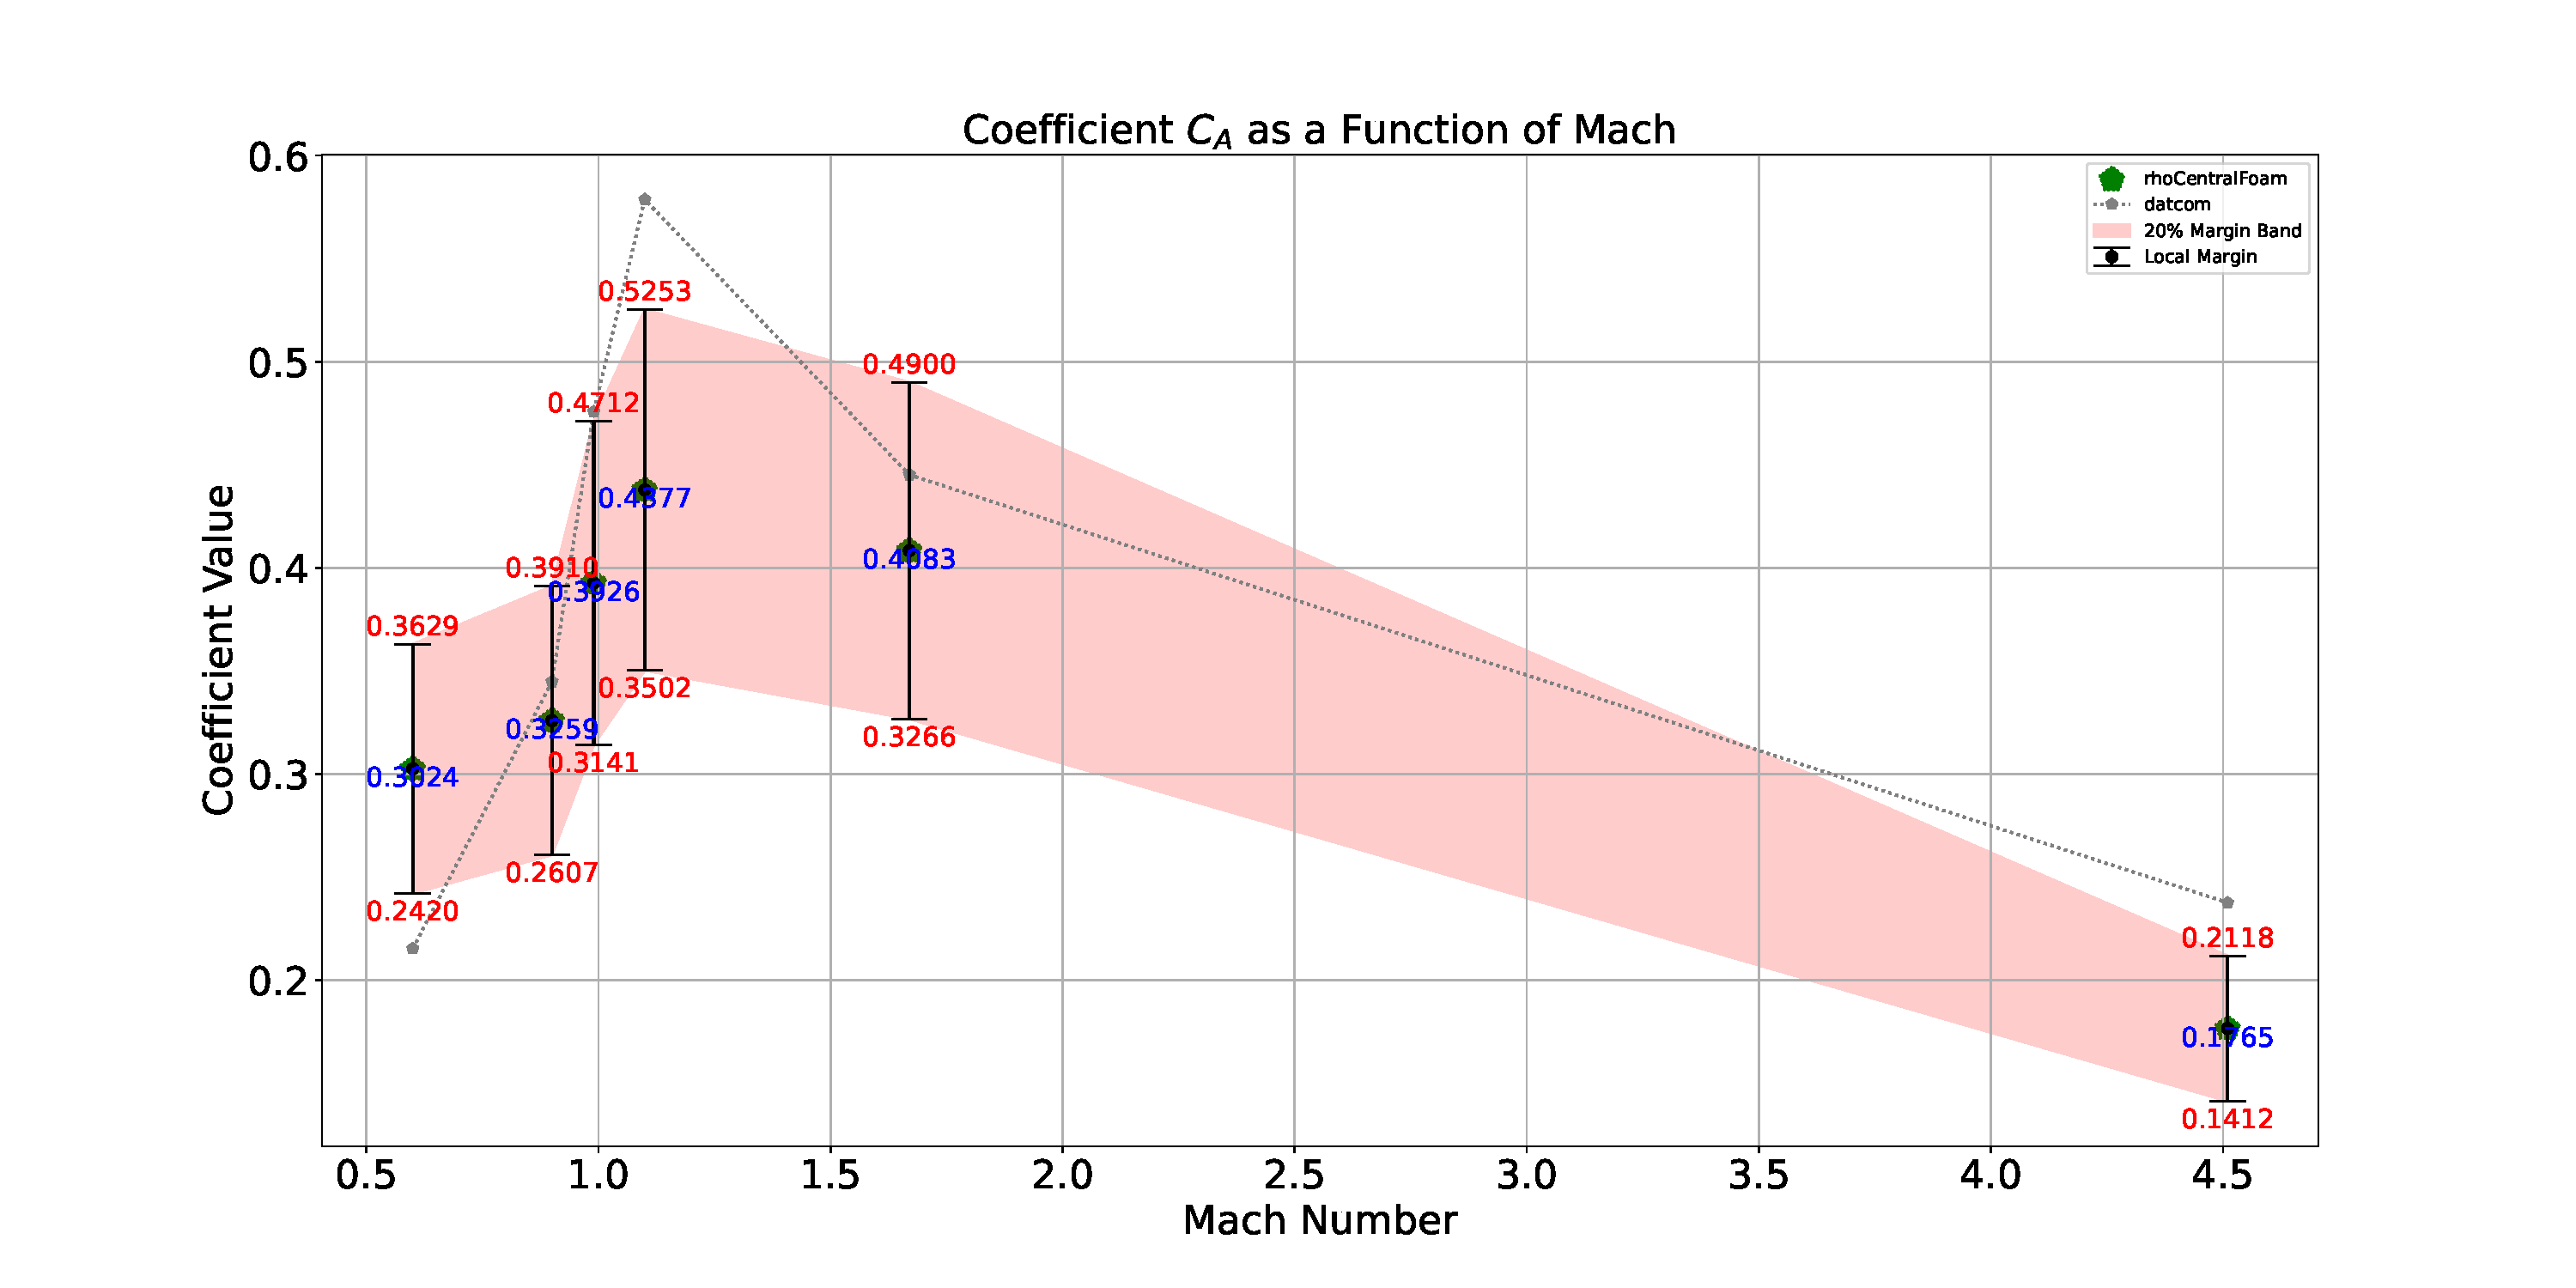
\includegraphics[width=0.995\linewidth]{figs/eris/S123F/fixed/Eris0_CA.pdf}\\
    \vspace{-0.4cm}
    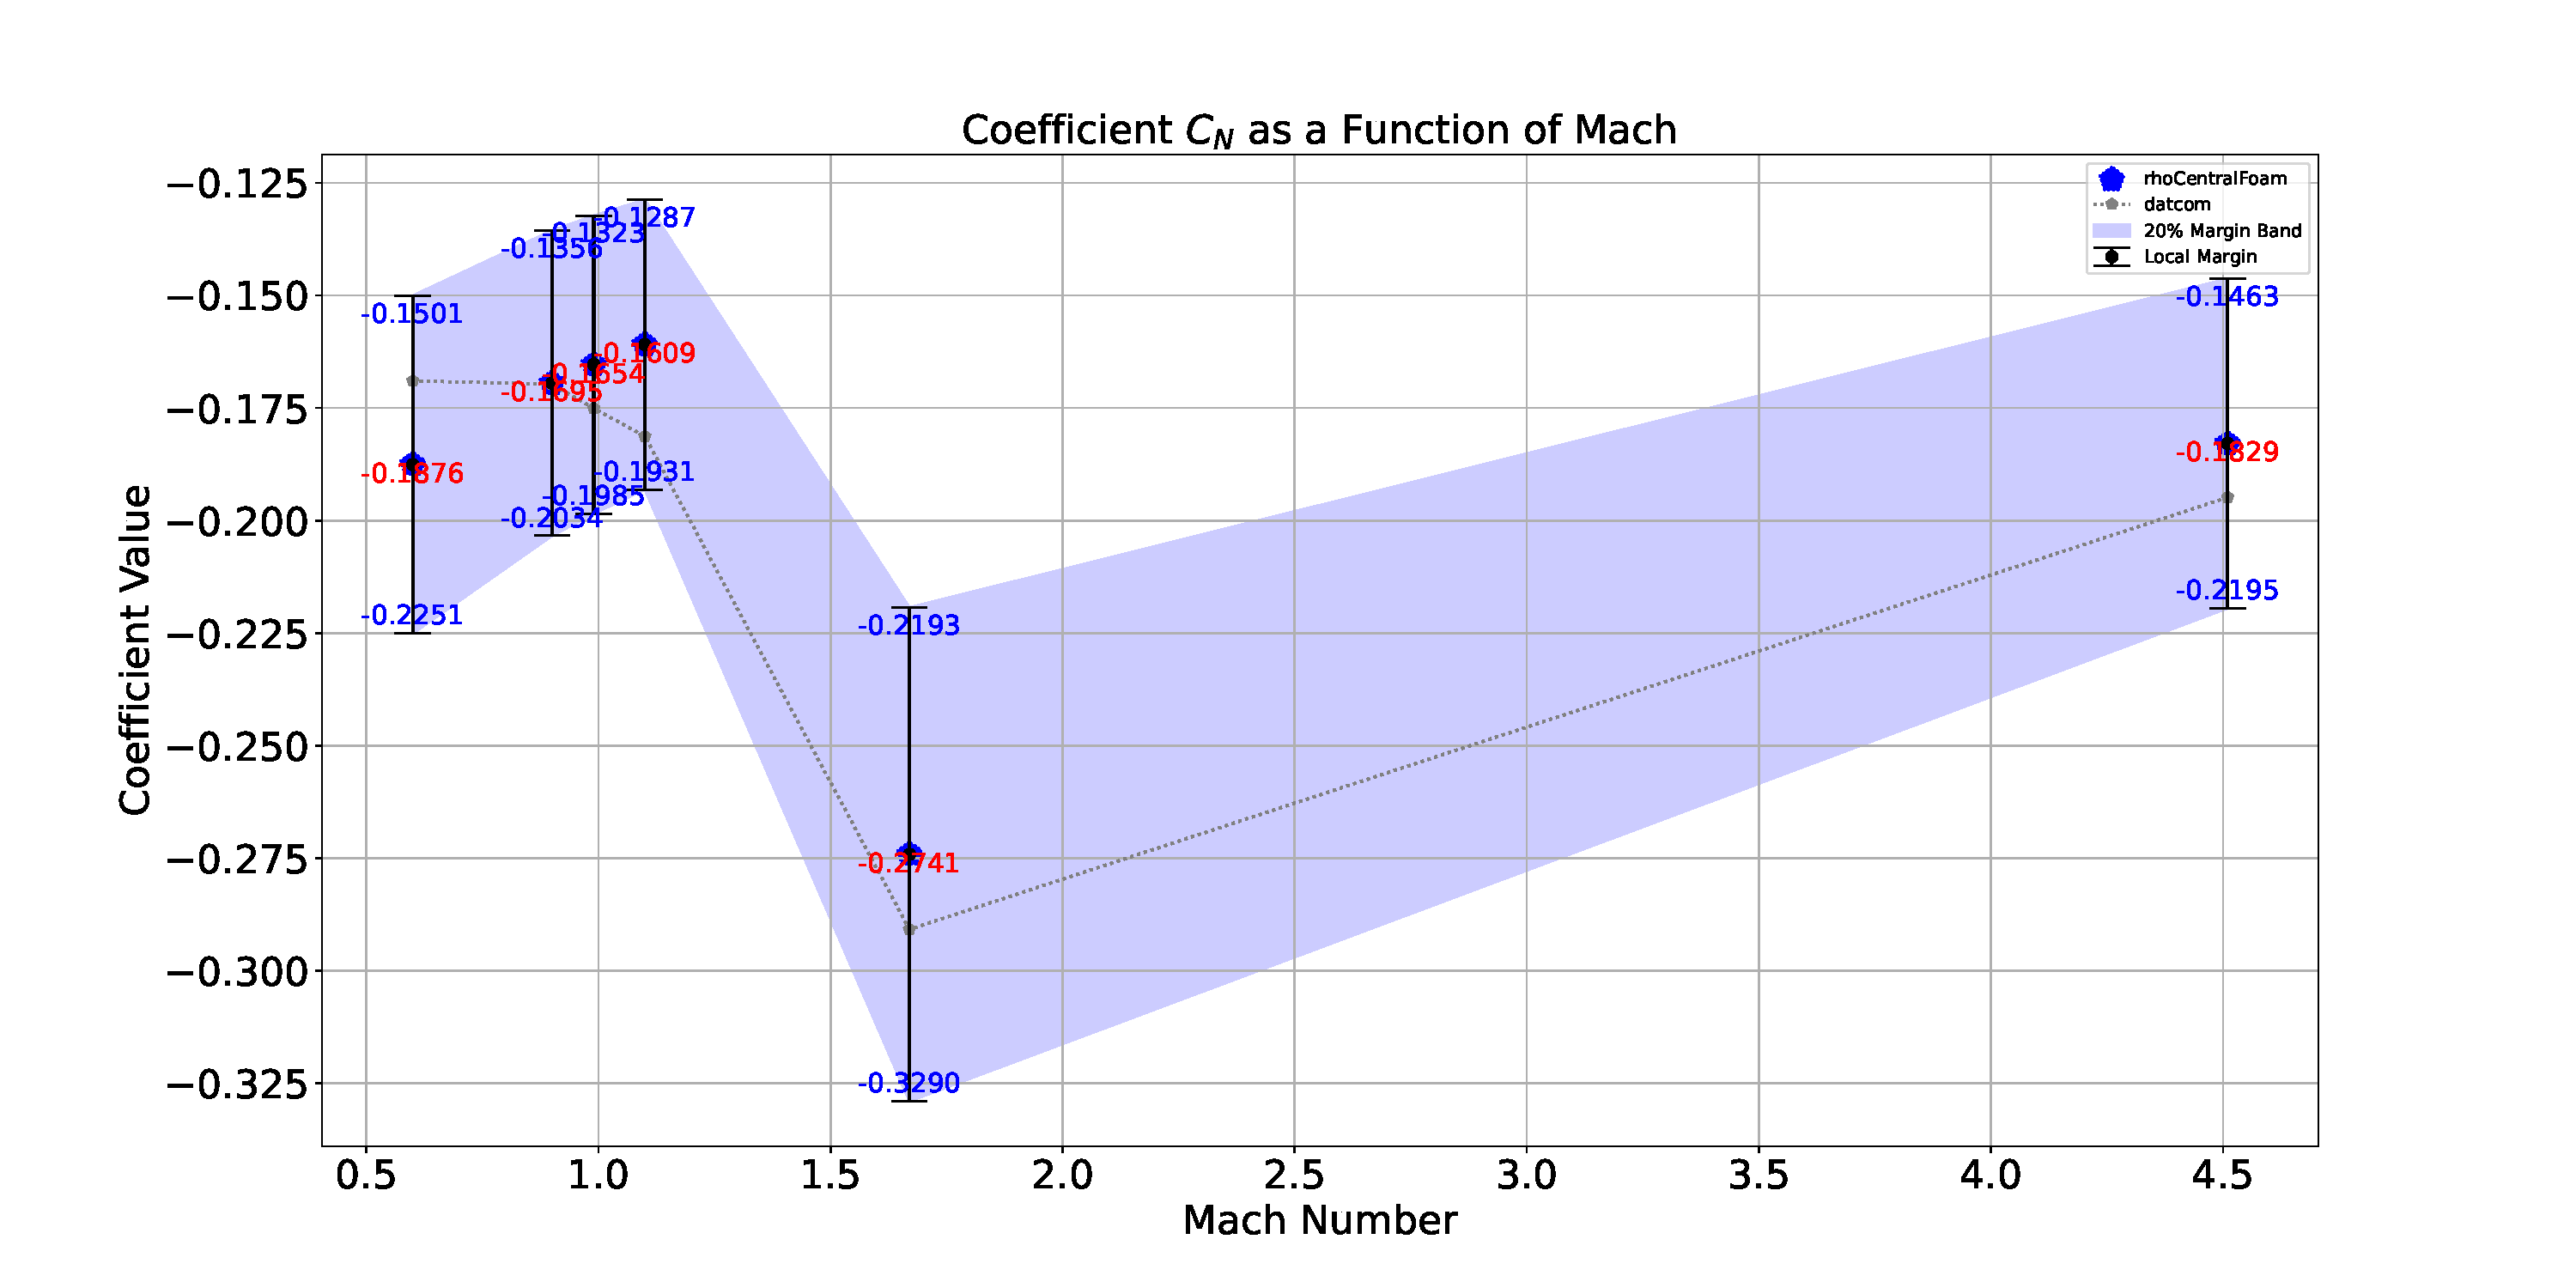
\includegraphics[width=0.995\linewidth]{figs/eris/S123F/fixed/Eris0_CN.pdf}\\
    \vspace{-0.4cm}
    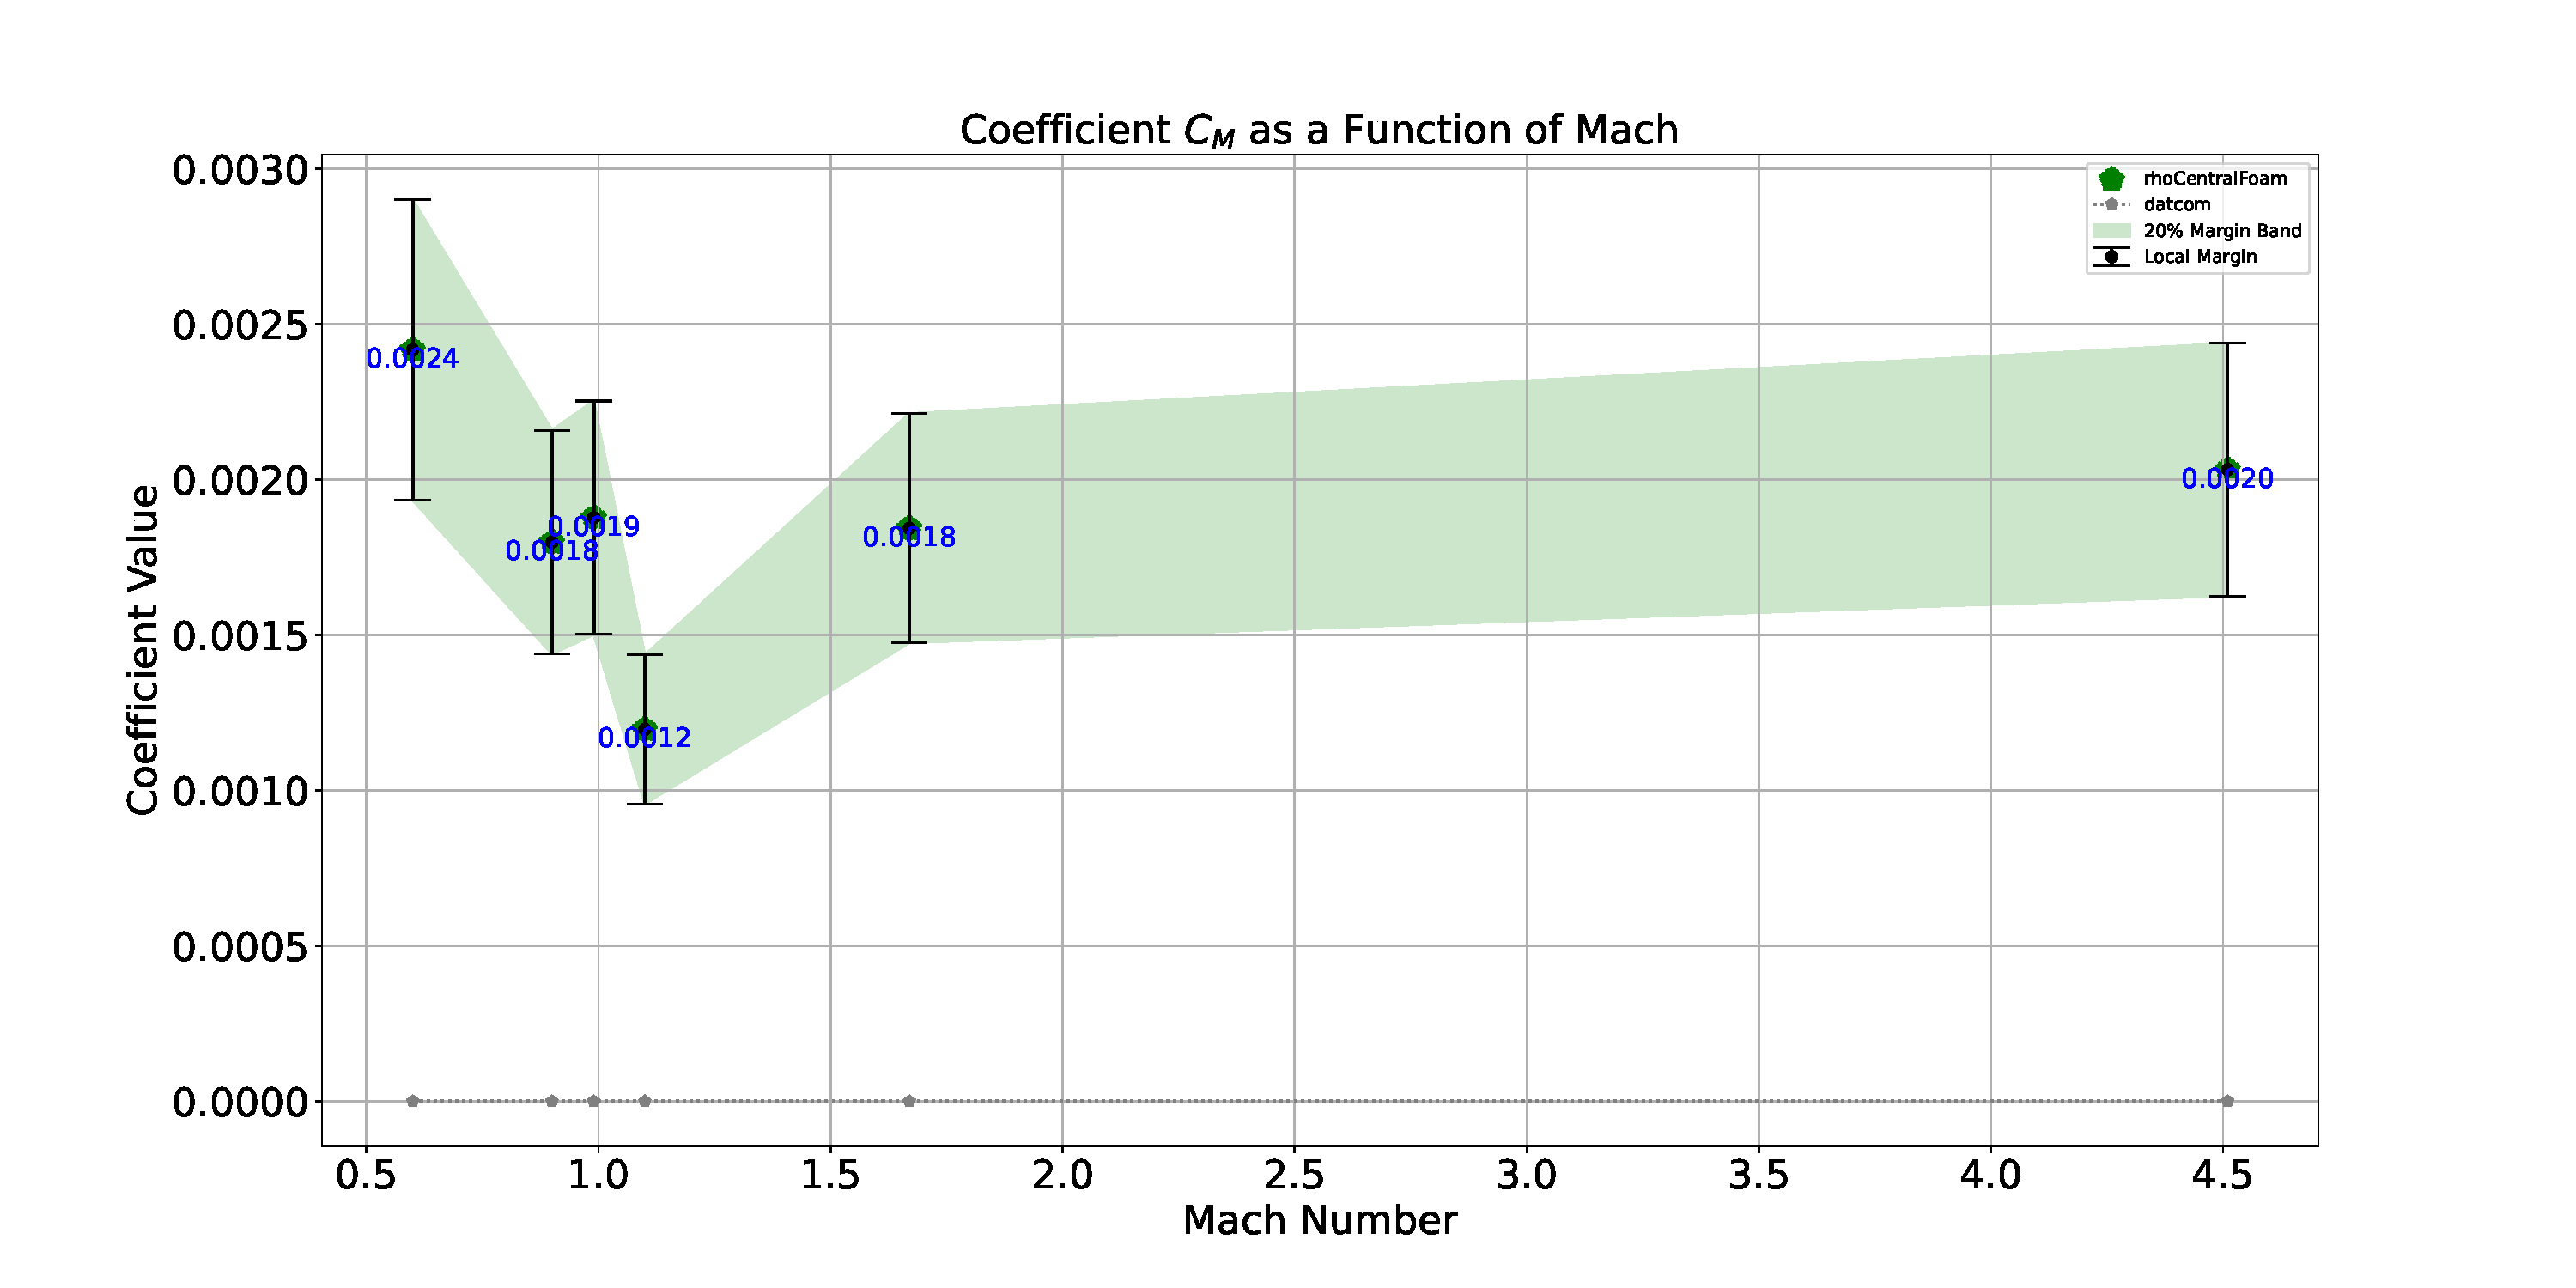
\includegraphics[width=0.995\linewidth]{figs/eris/S123F/fixed/Eris0_CM.pdf}
    \caption{Aerodynamic coefficients, $C_A$, $C_N$, $C_M$, for the Eris Block 1.1 Rev. A configuration \textbf{S123F} launch vehicle as a function of Mach number for an angle of attack \hl{$\alpha$ = 0$^\circ$}. The applied uncertainty margin was imported from the benchmark validation test case ARCAS.}
    \label{fig:eris-CA-CA-CM_alpha0}
\end{figure}
%
%\begin{figure}[H]
%    \centering
%    %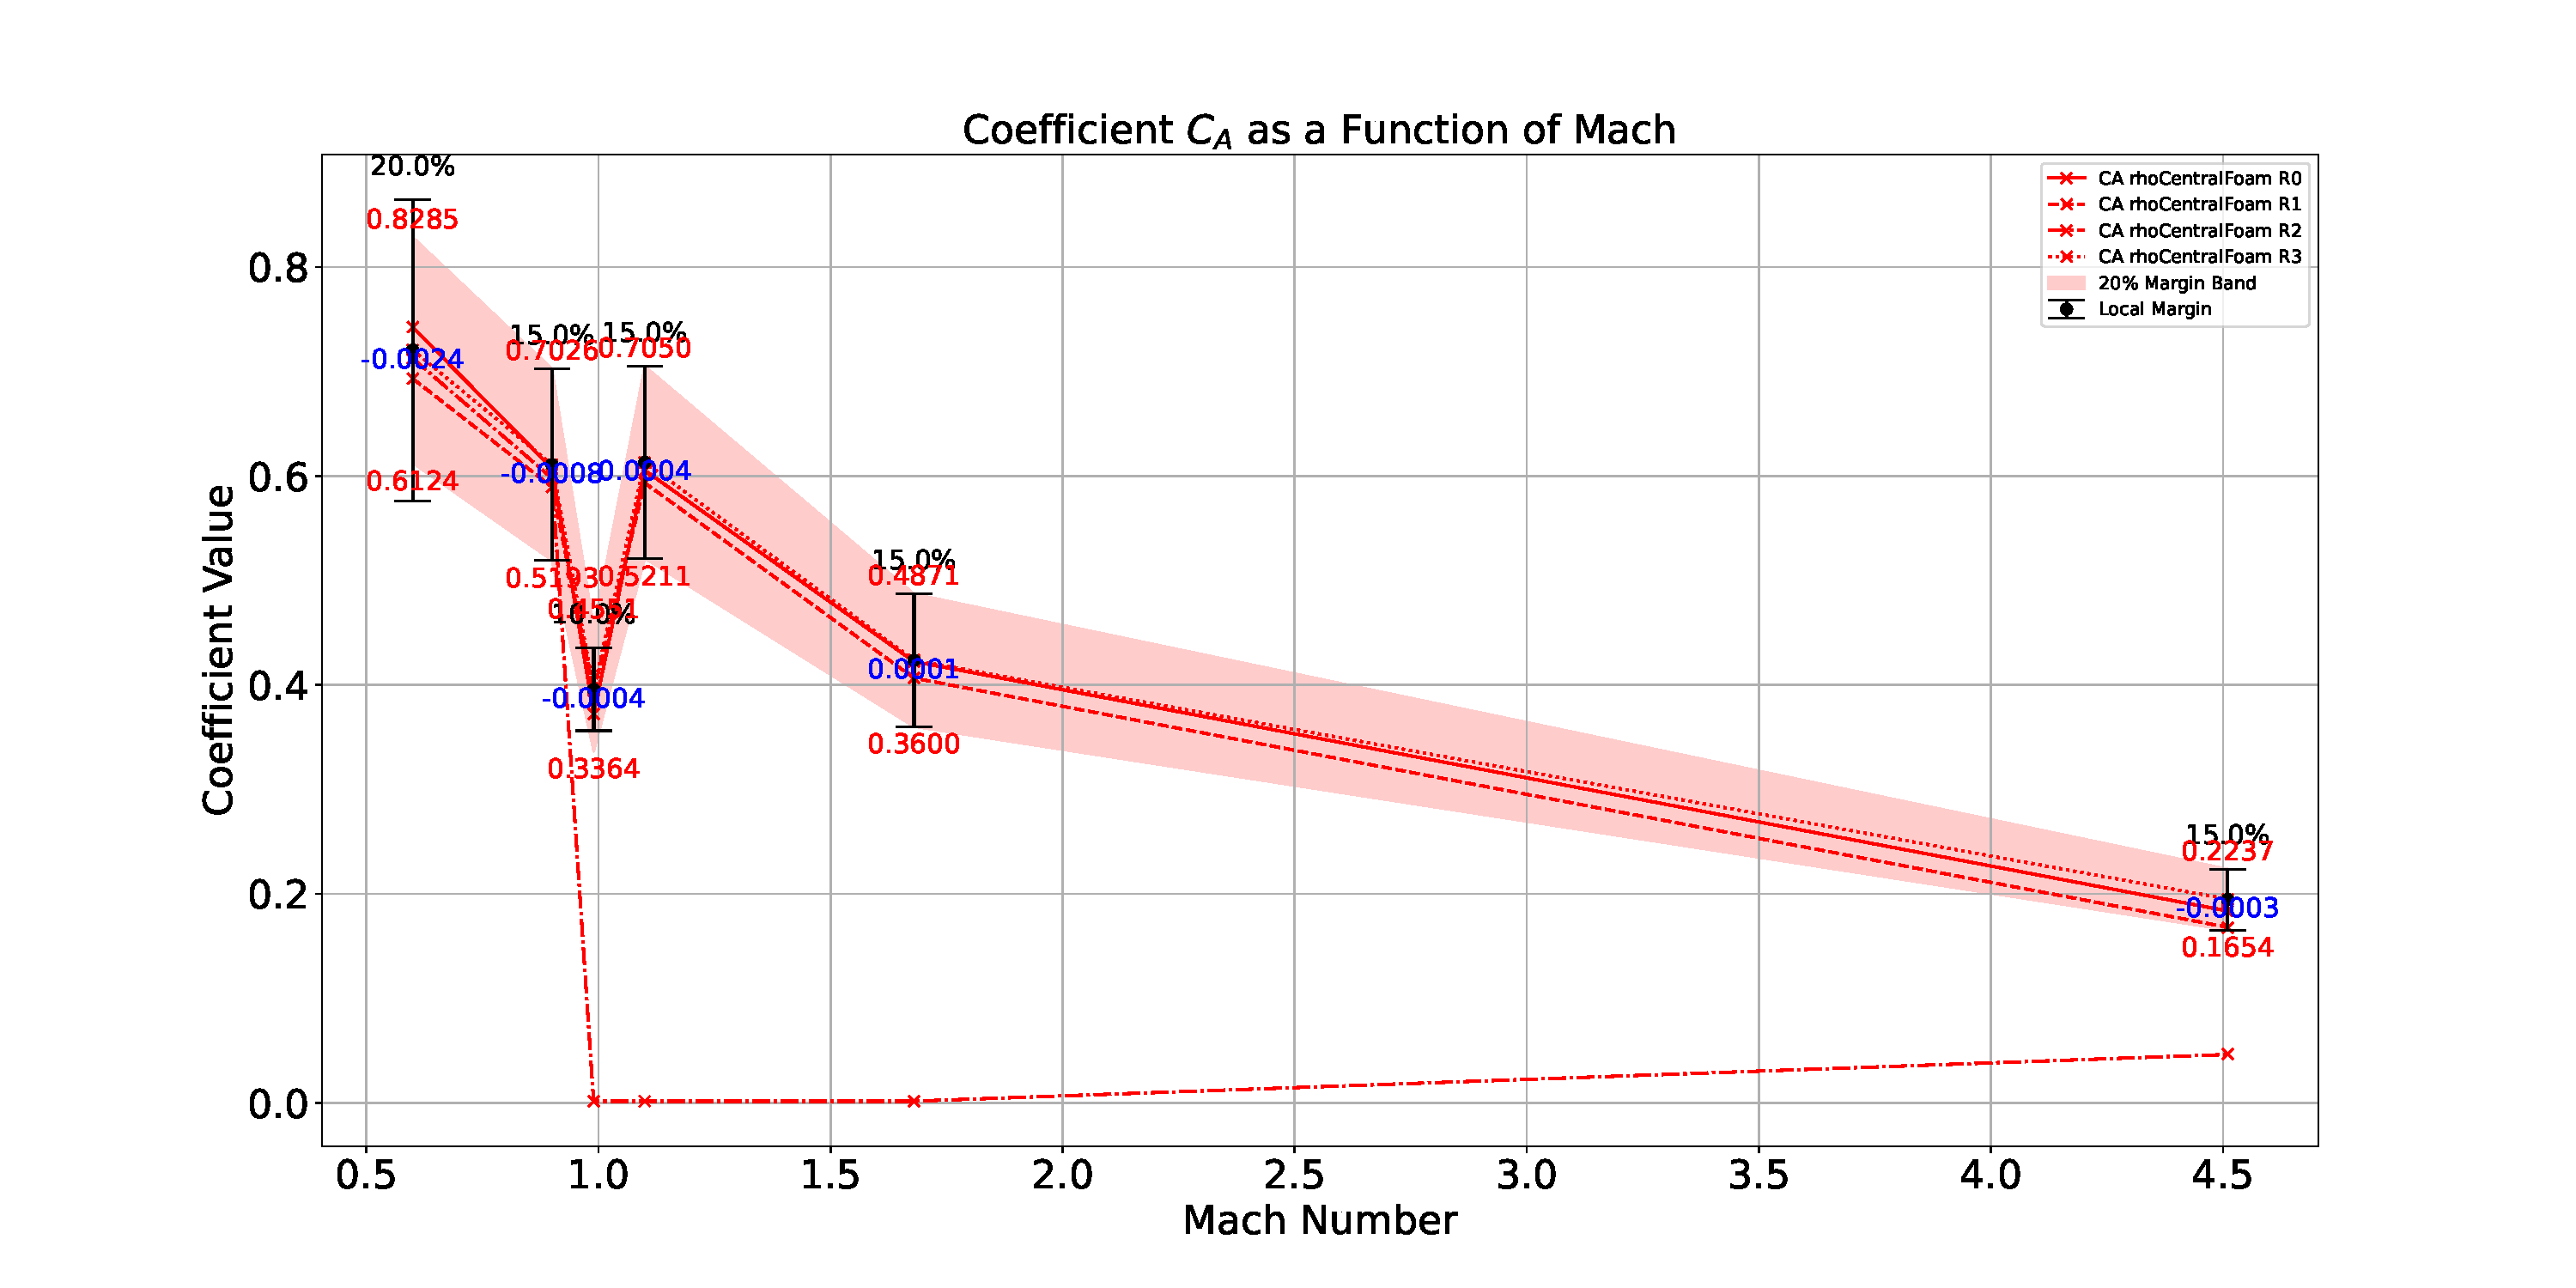
\includegraphics[width=0.995\linewidth]{figs/eris/eris_CA.pdf}\\
%    %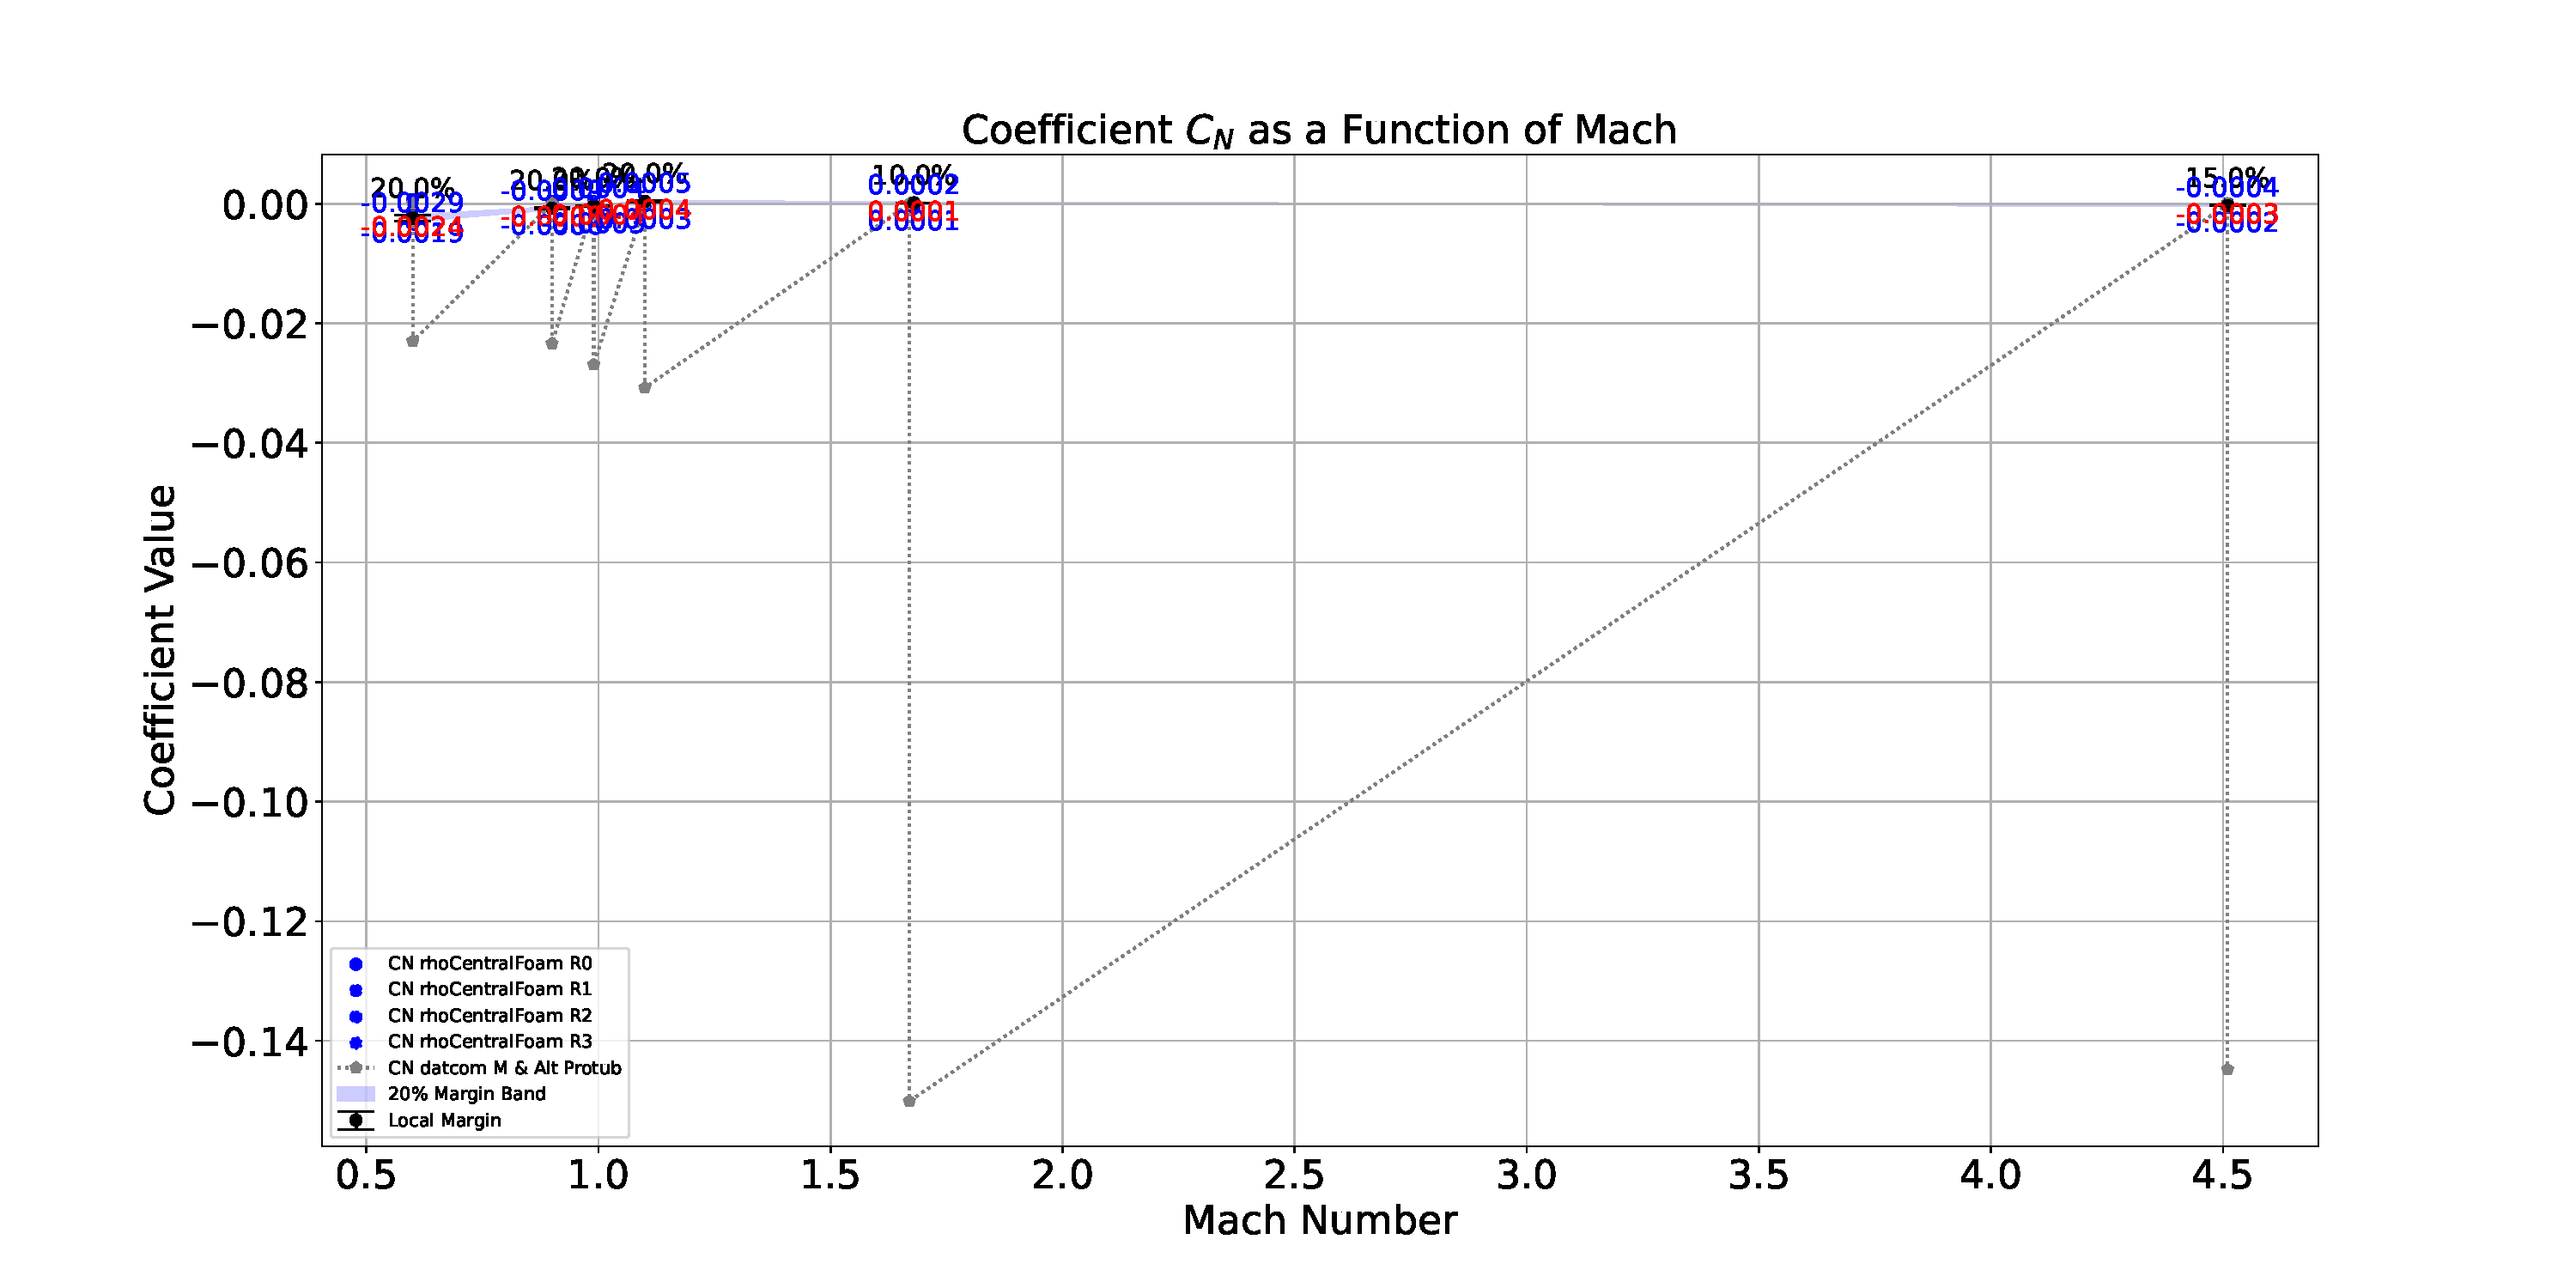
\includegraphics[width=0.995\linewidth]{figs/eris/eris_CN.pdf}\\
%    %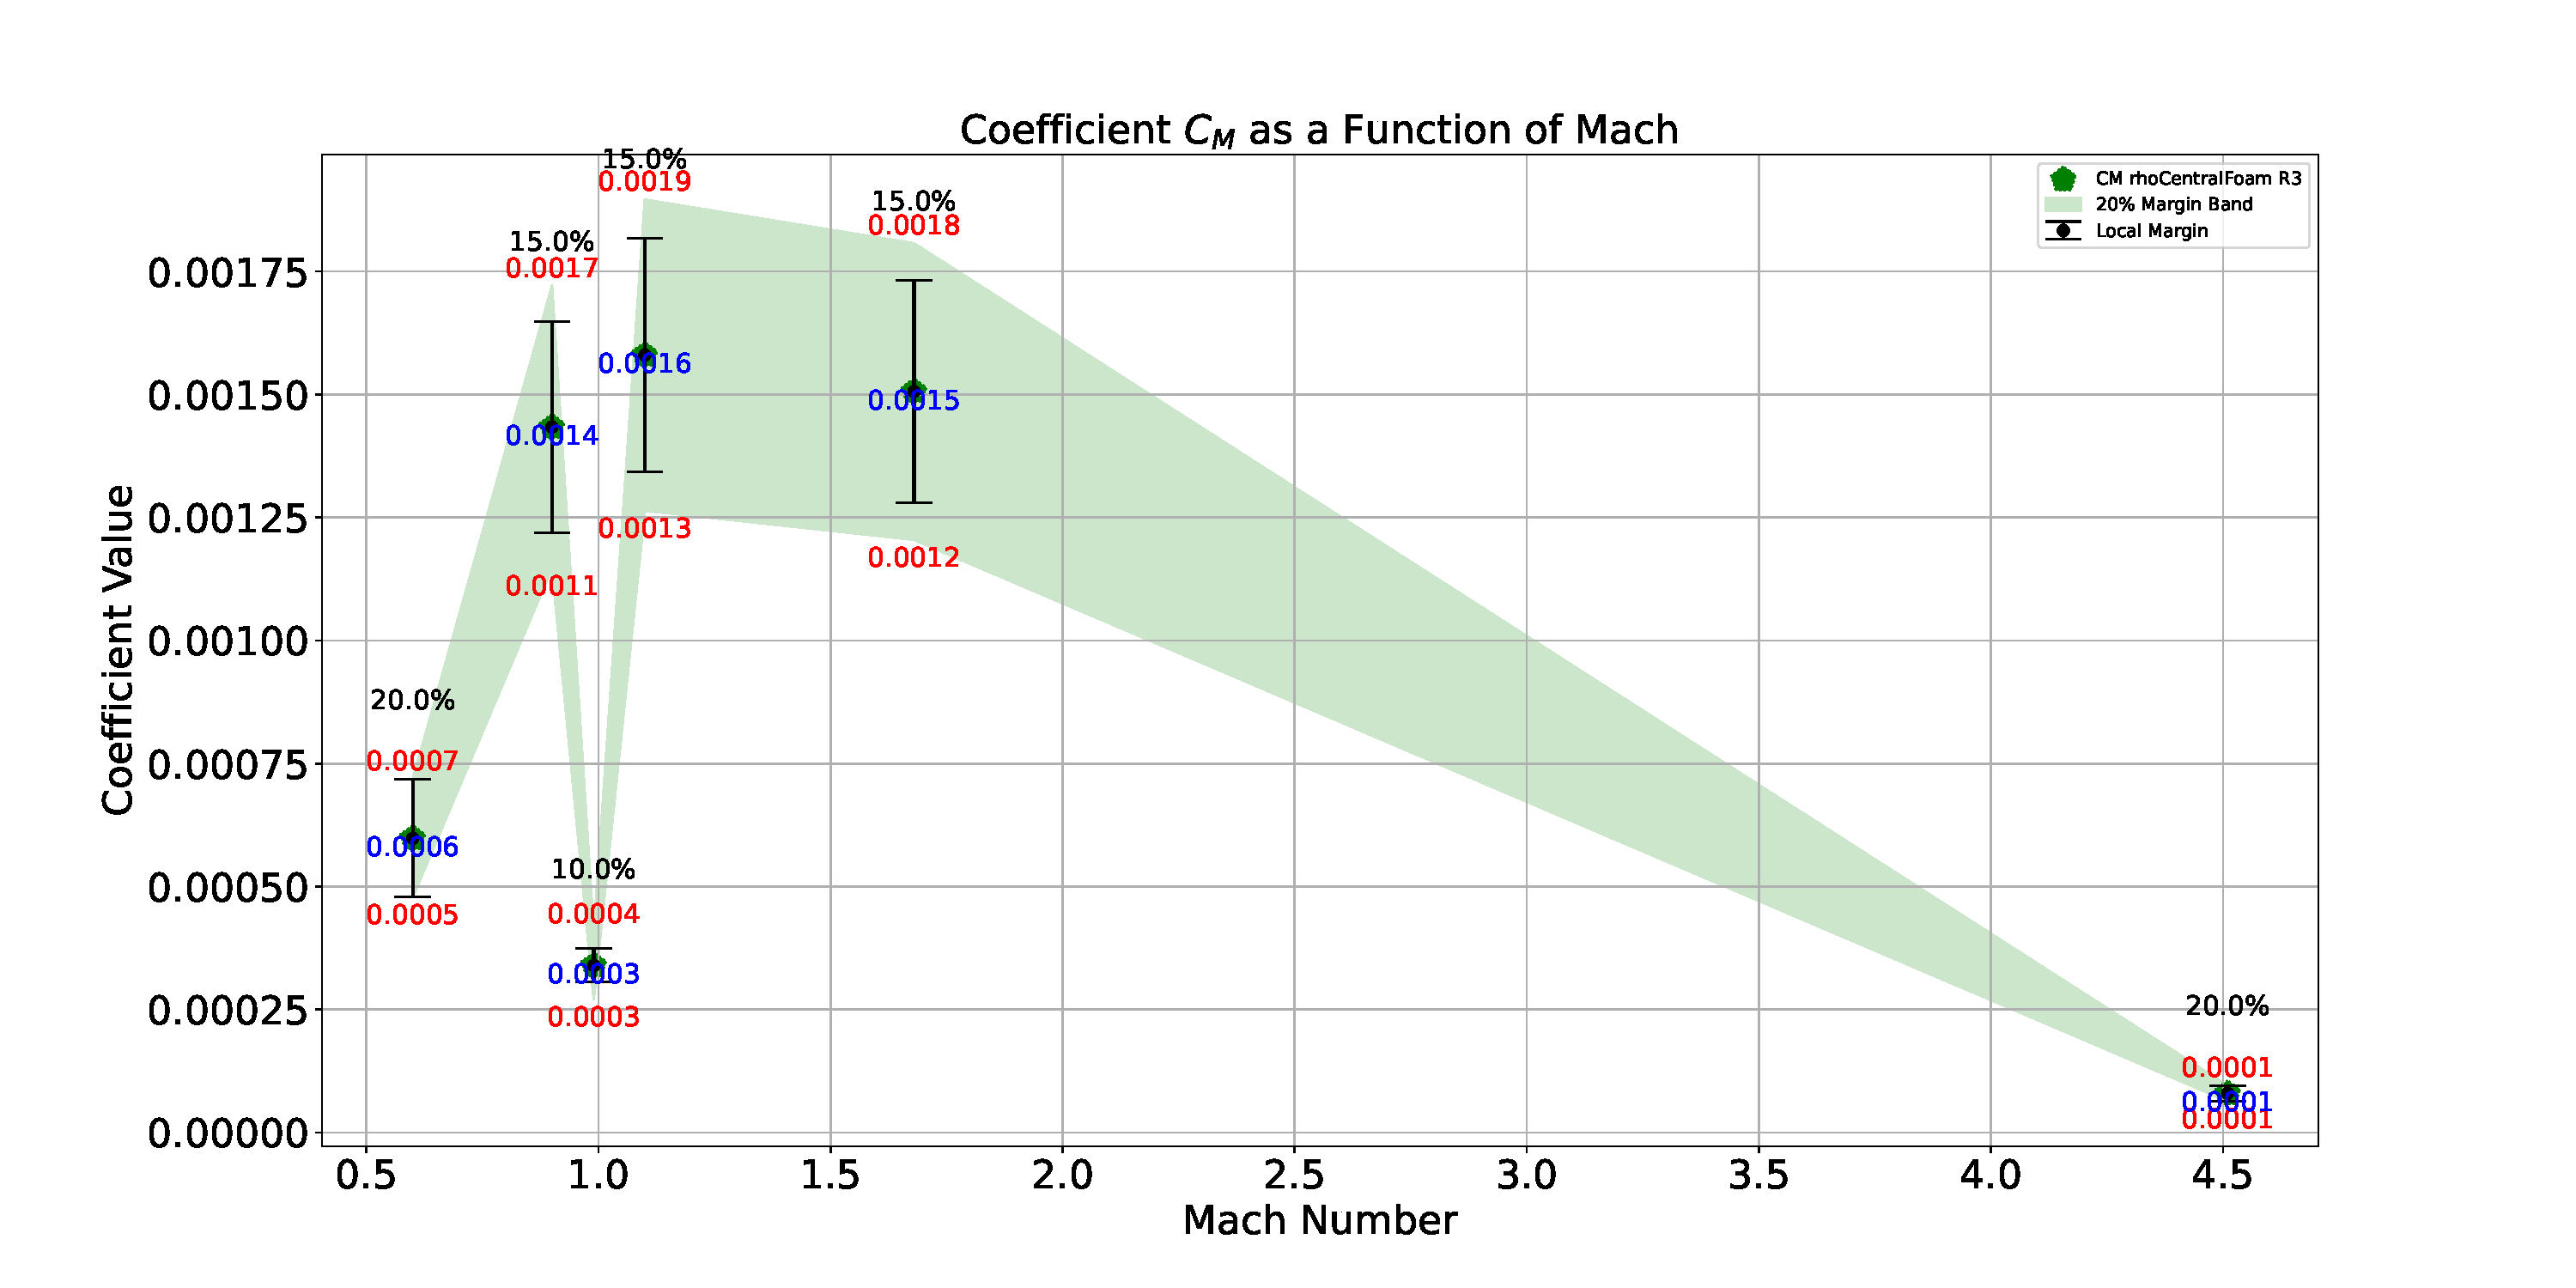
\includegraphics[width=0.995\linewidth]{figs/eris/eris_CM.pdf}
%    %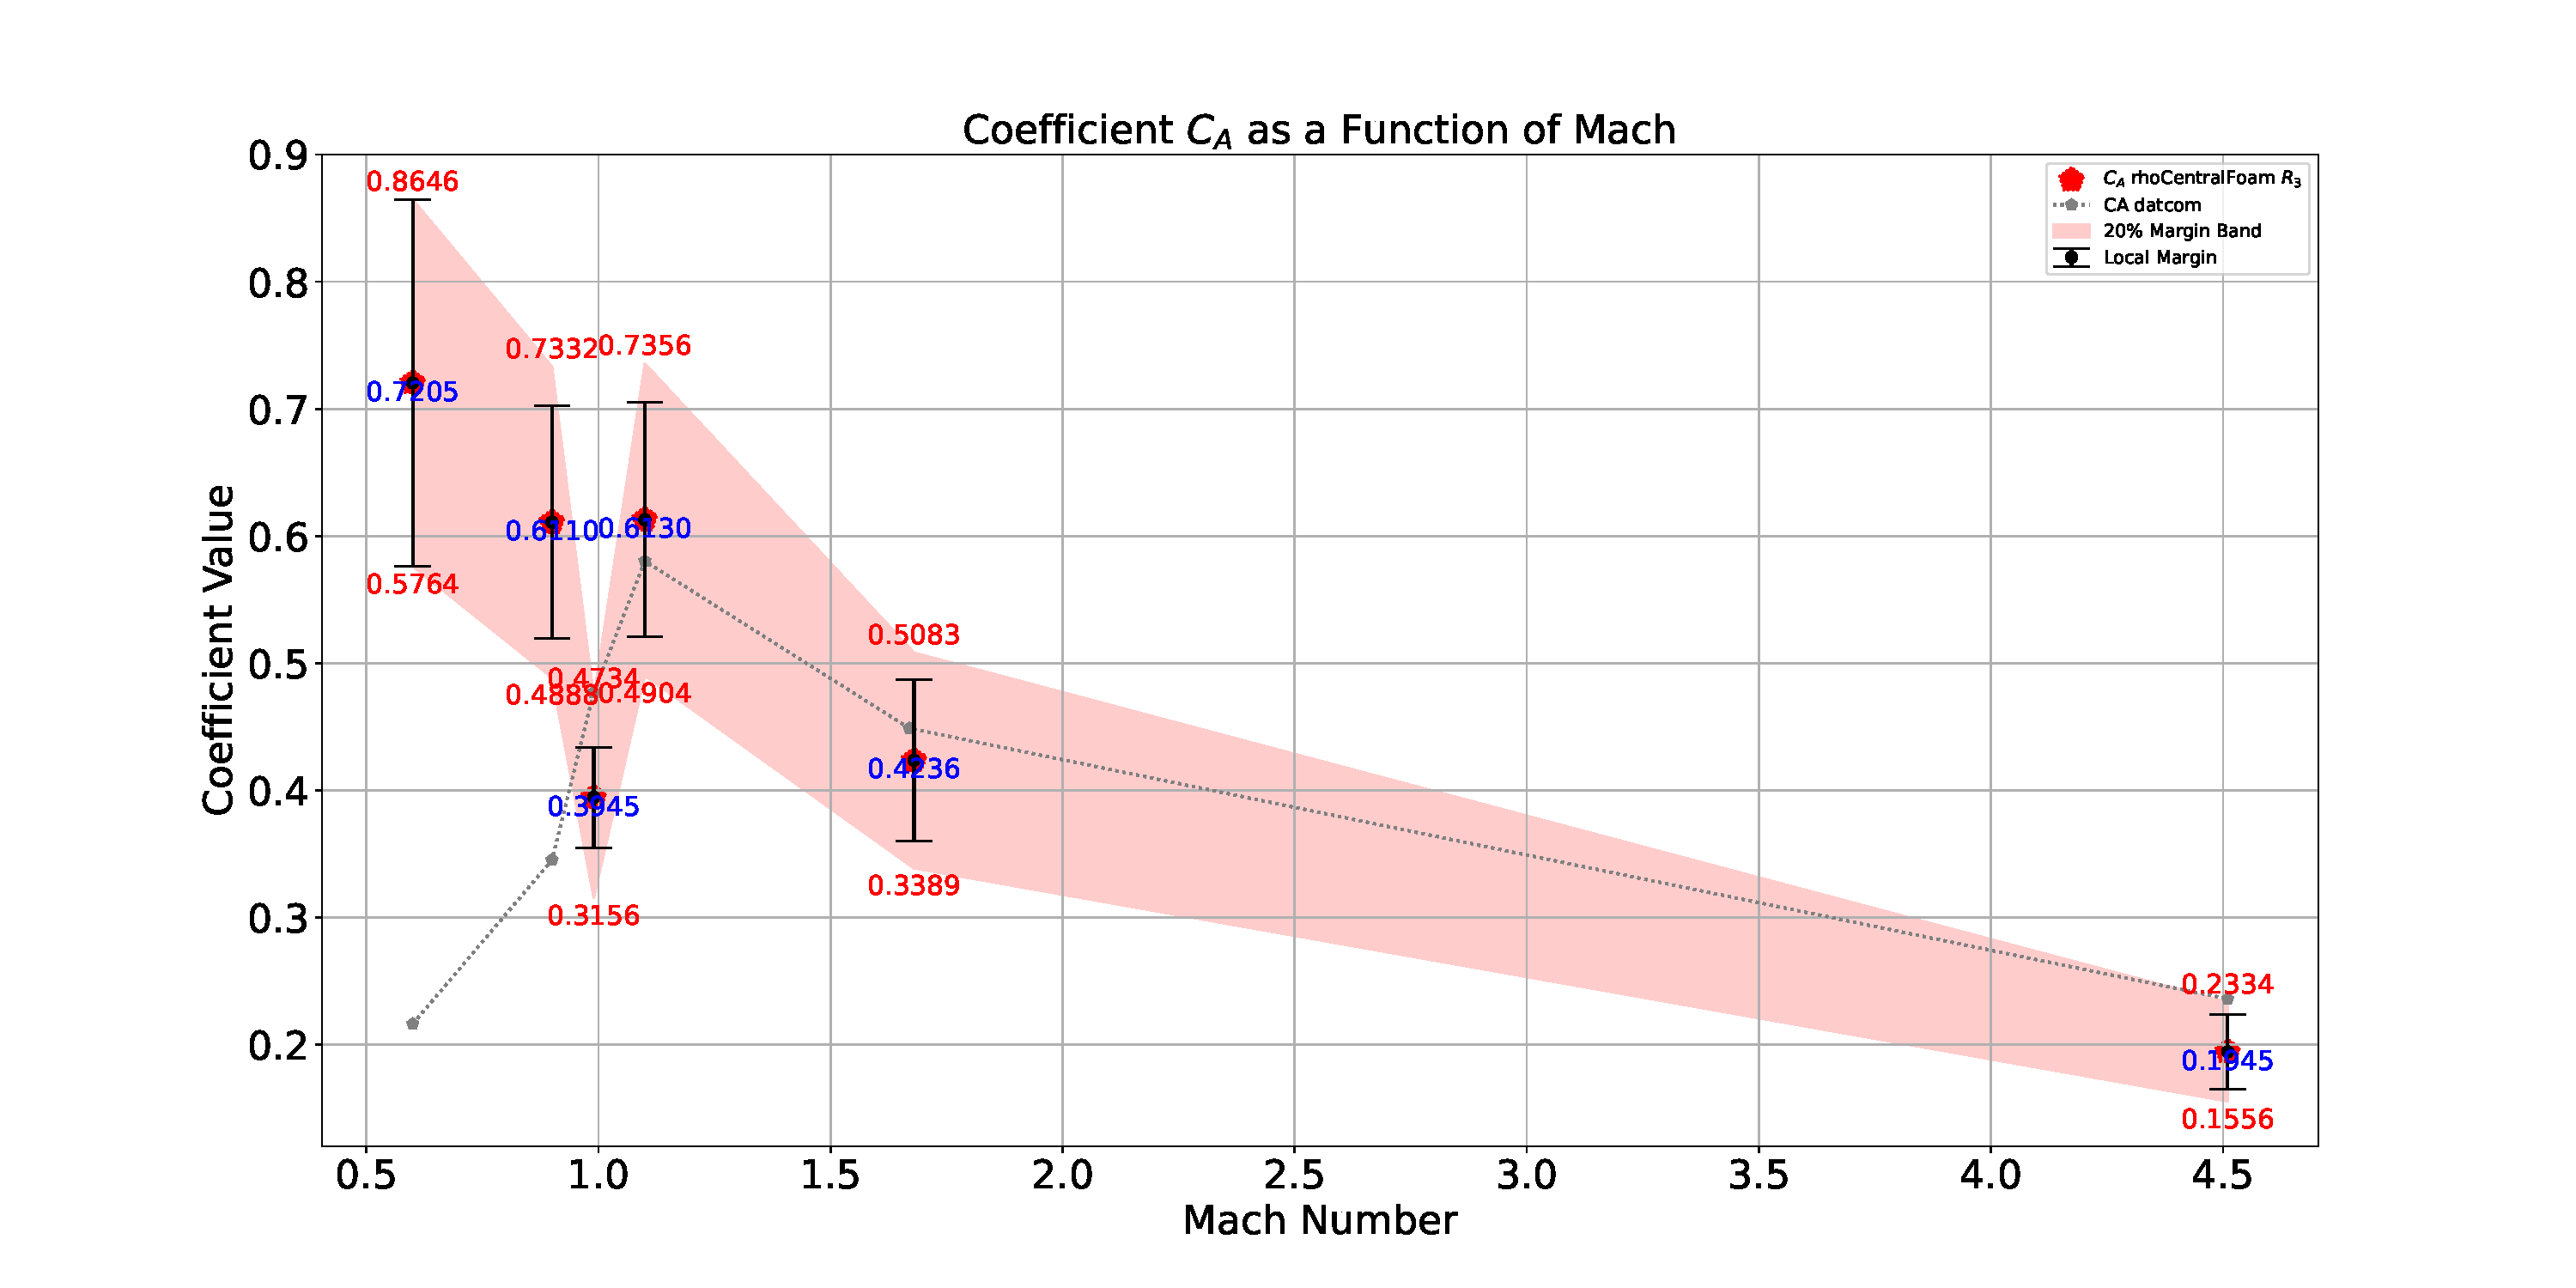
\includegraphics[width=0.995\linewidth]{figs/eris/eris0_CA.pdf}\\
%    %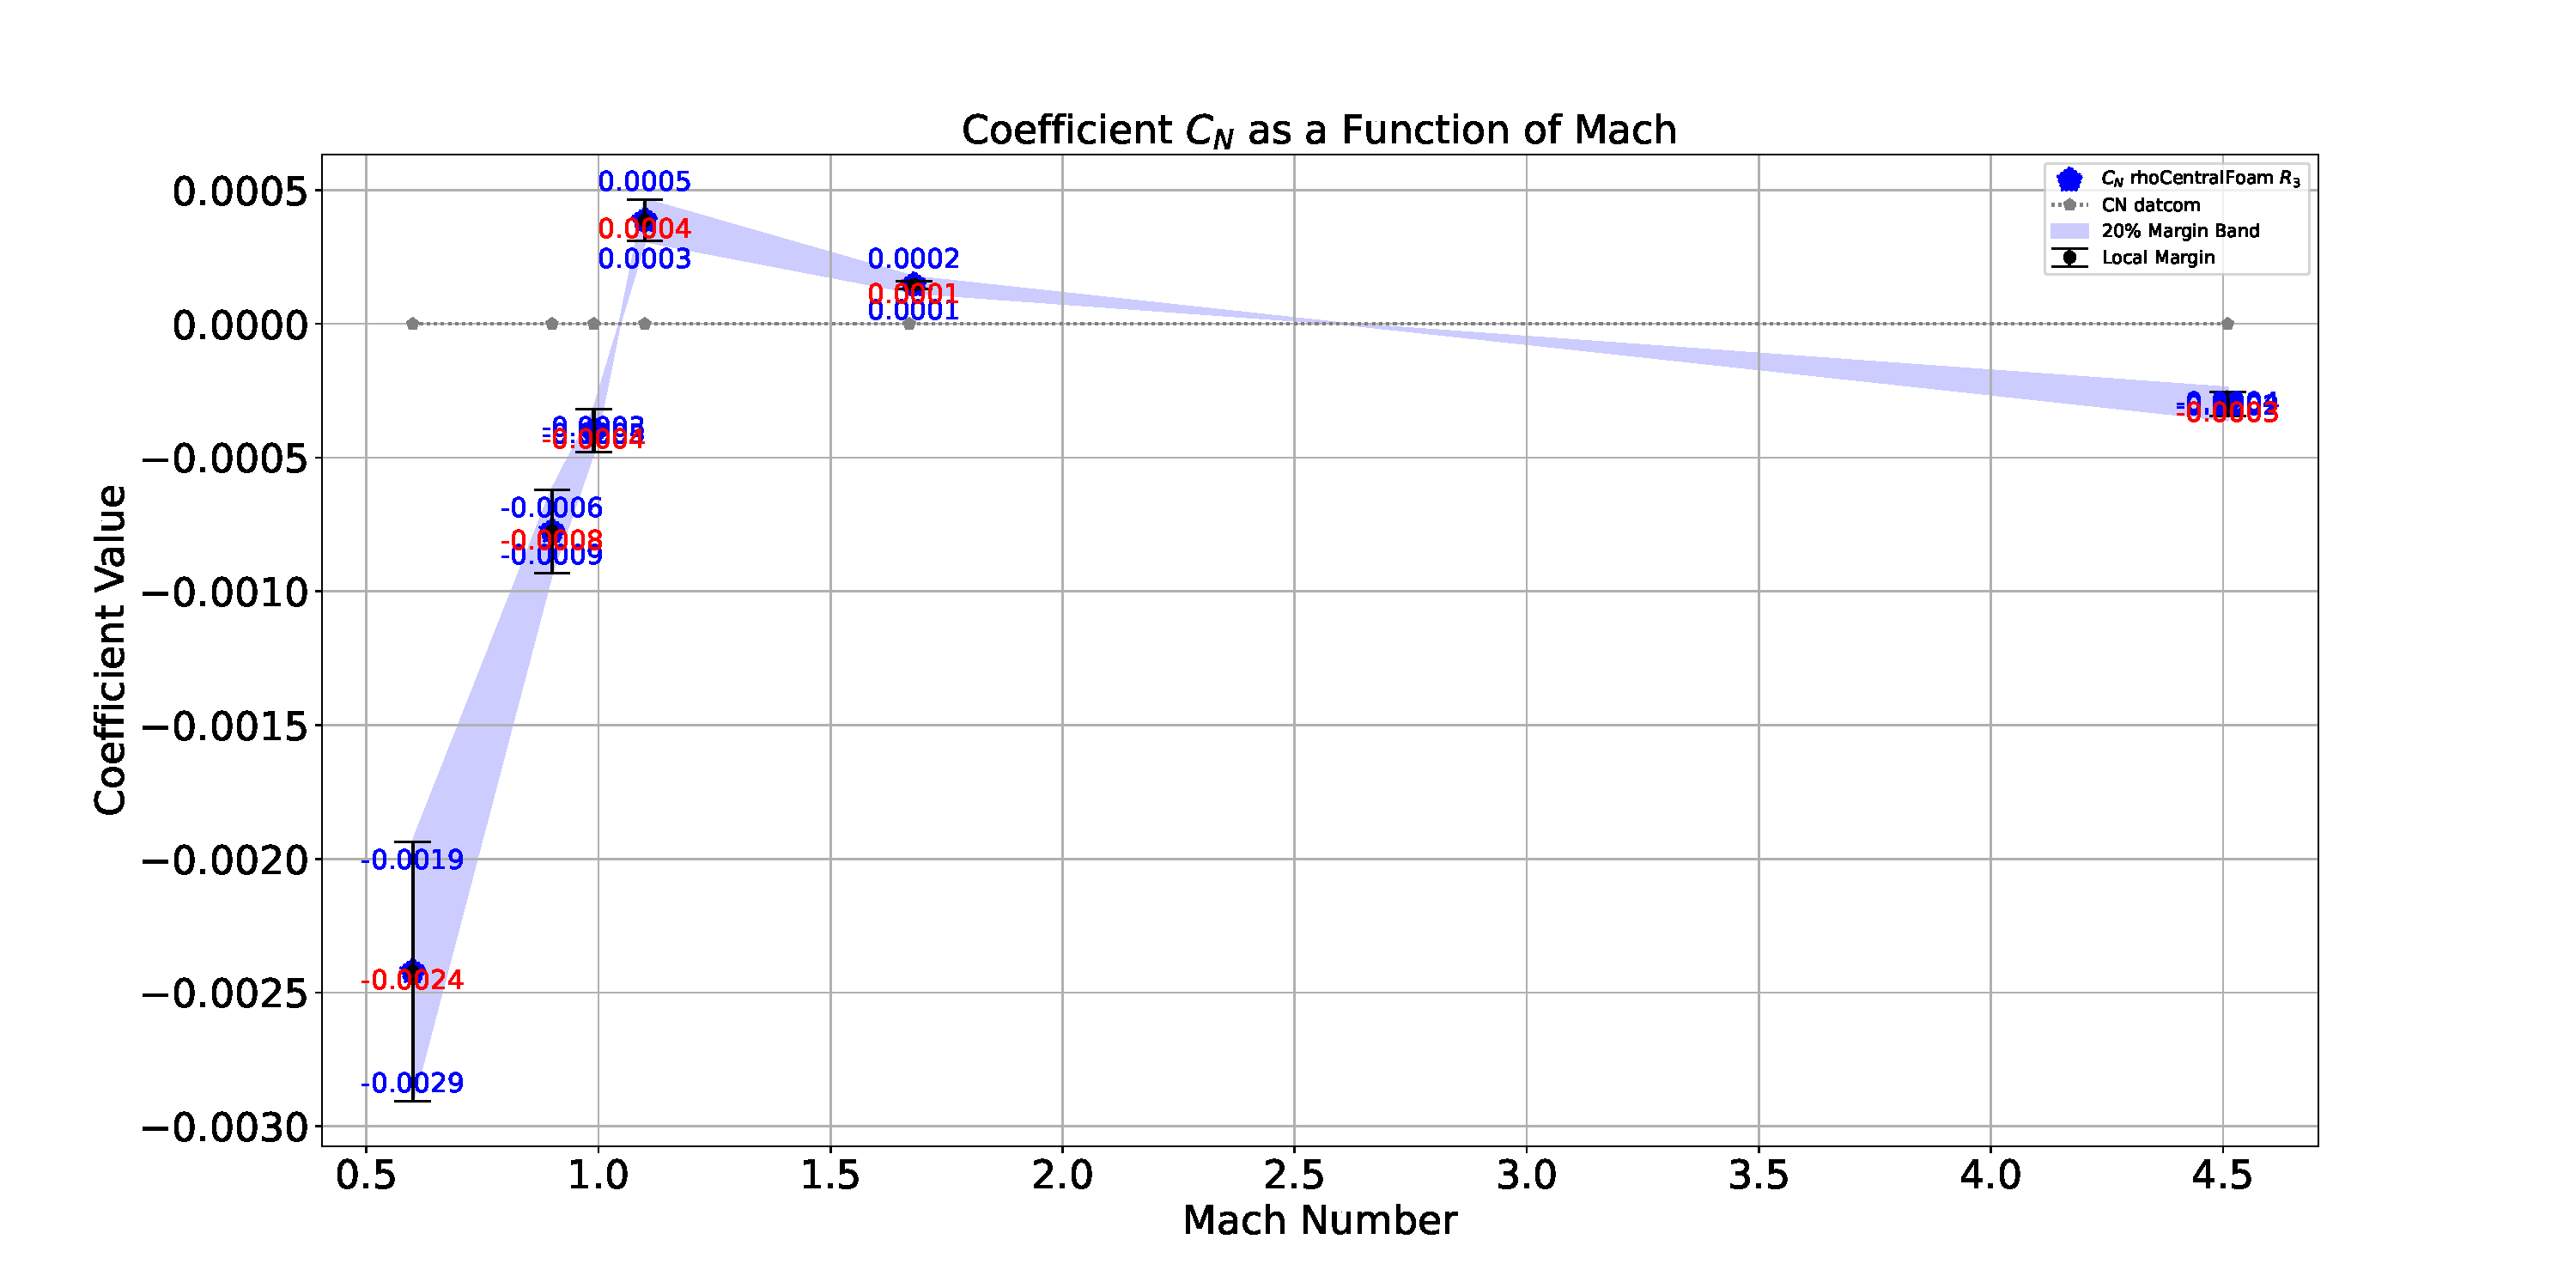
\includegraphics[width=0.995\linewidth]{figs/eris/eris0_CN.pdf}\\
%    %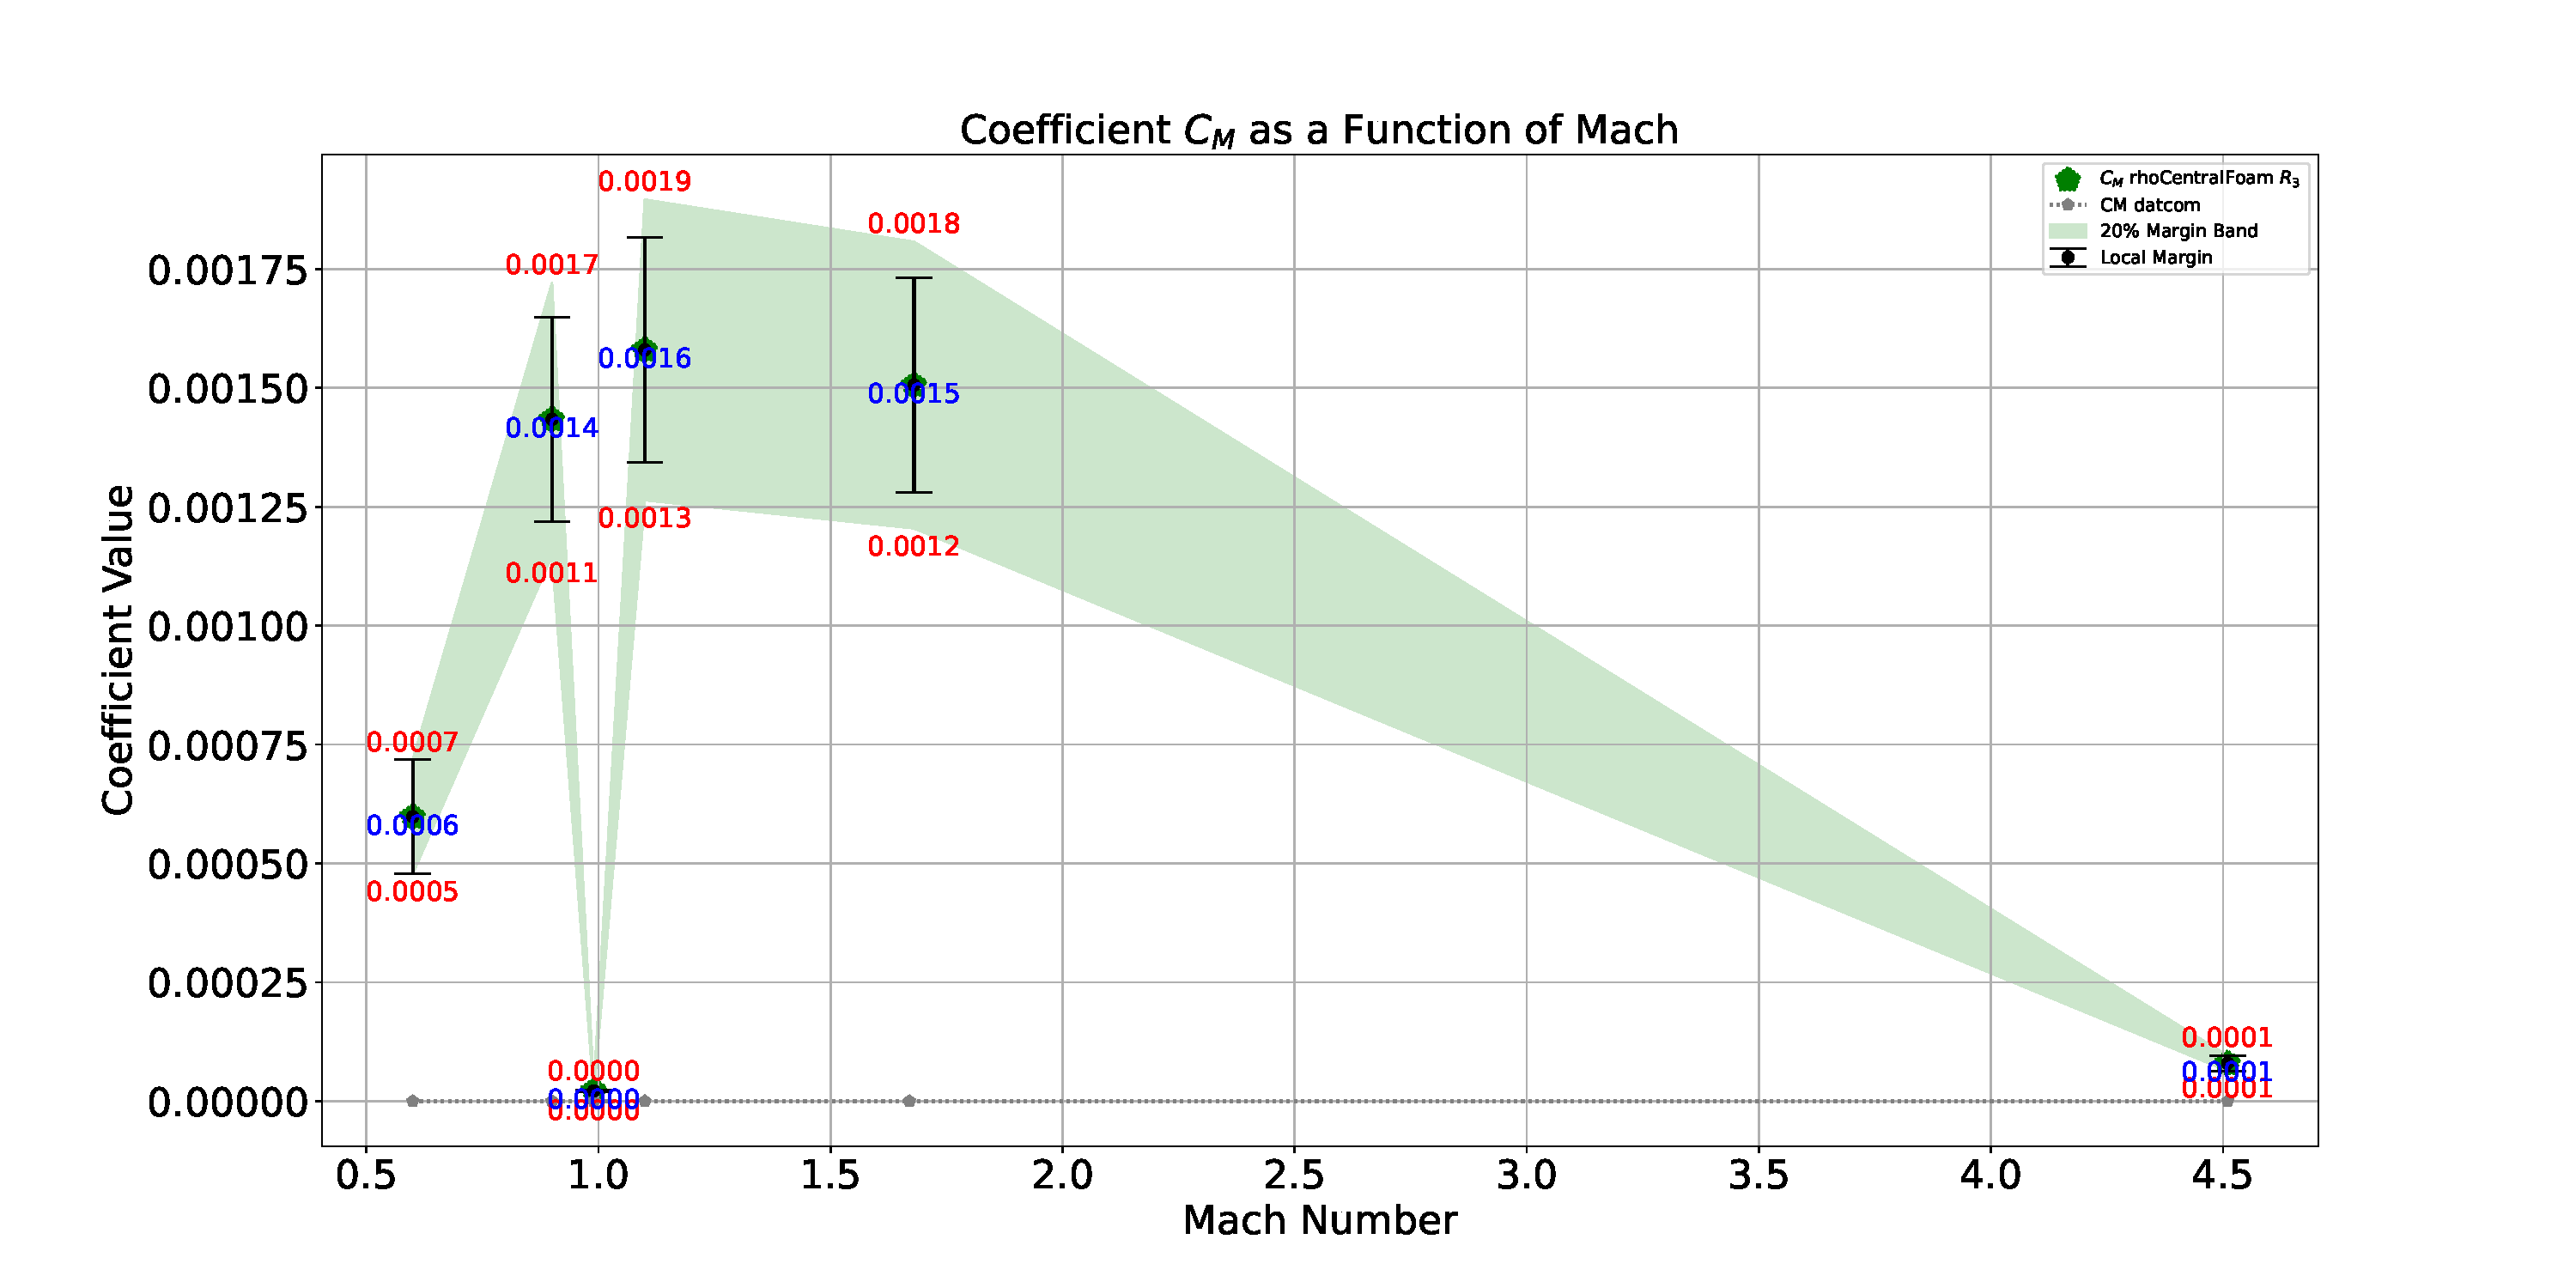
\includegraphics[width=0.995\linewidth]{figs/eris/eris0_CM.pdf}\\
%    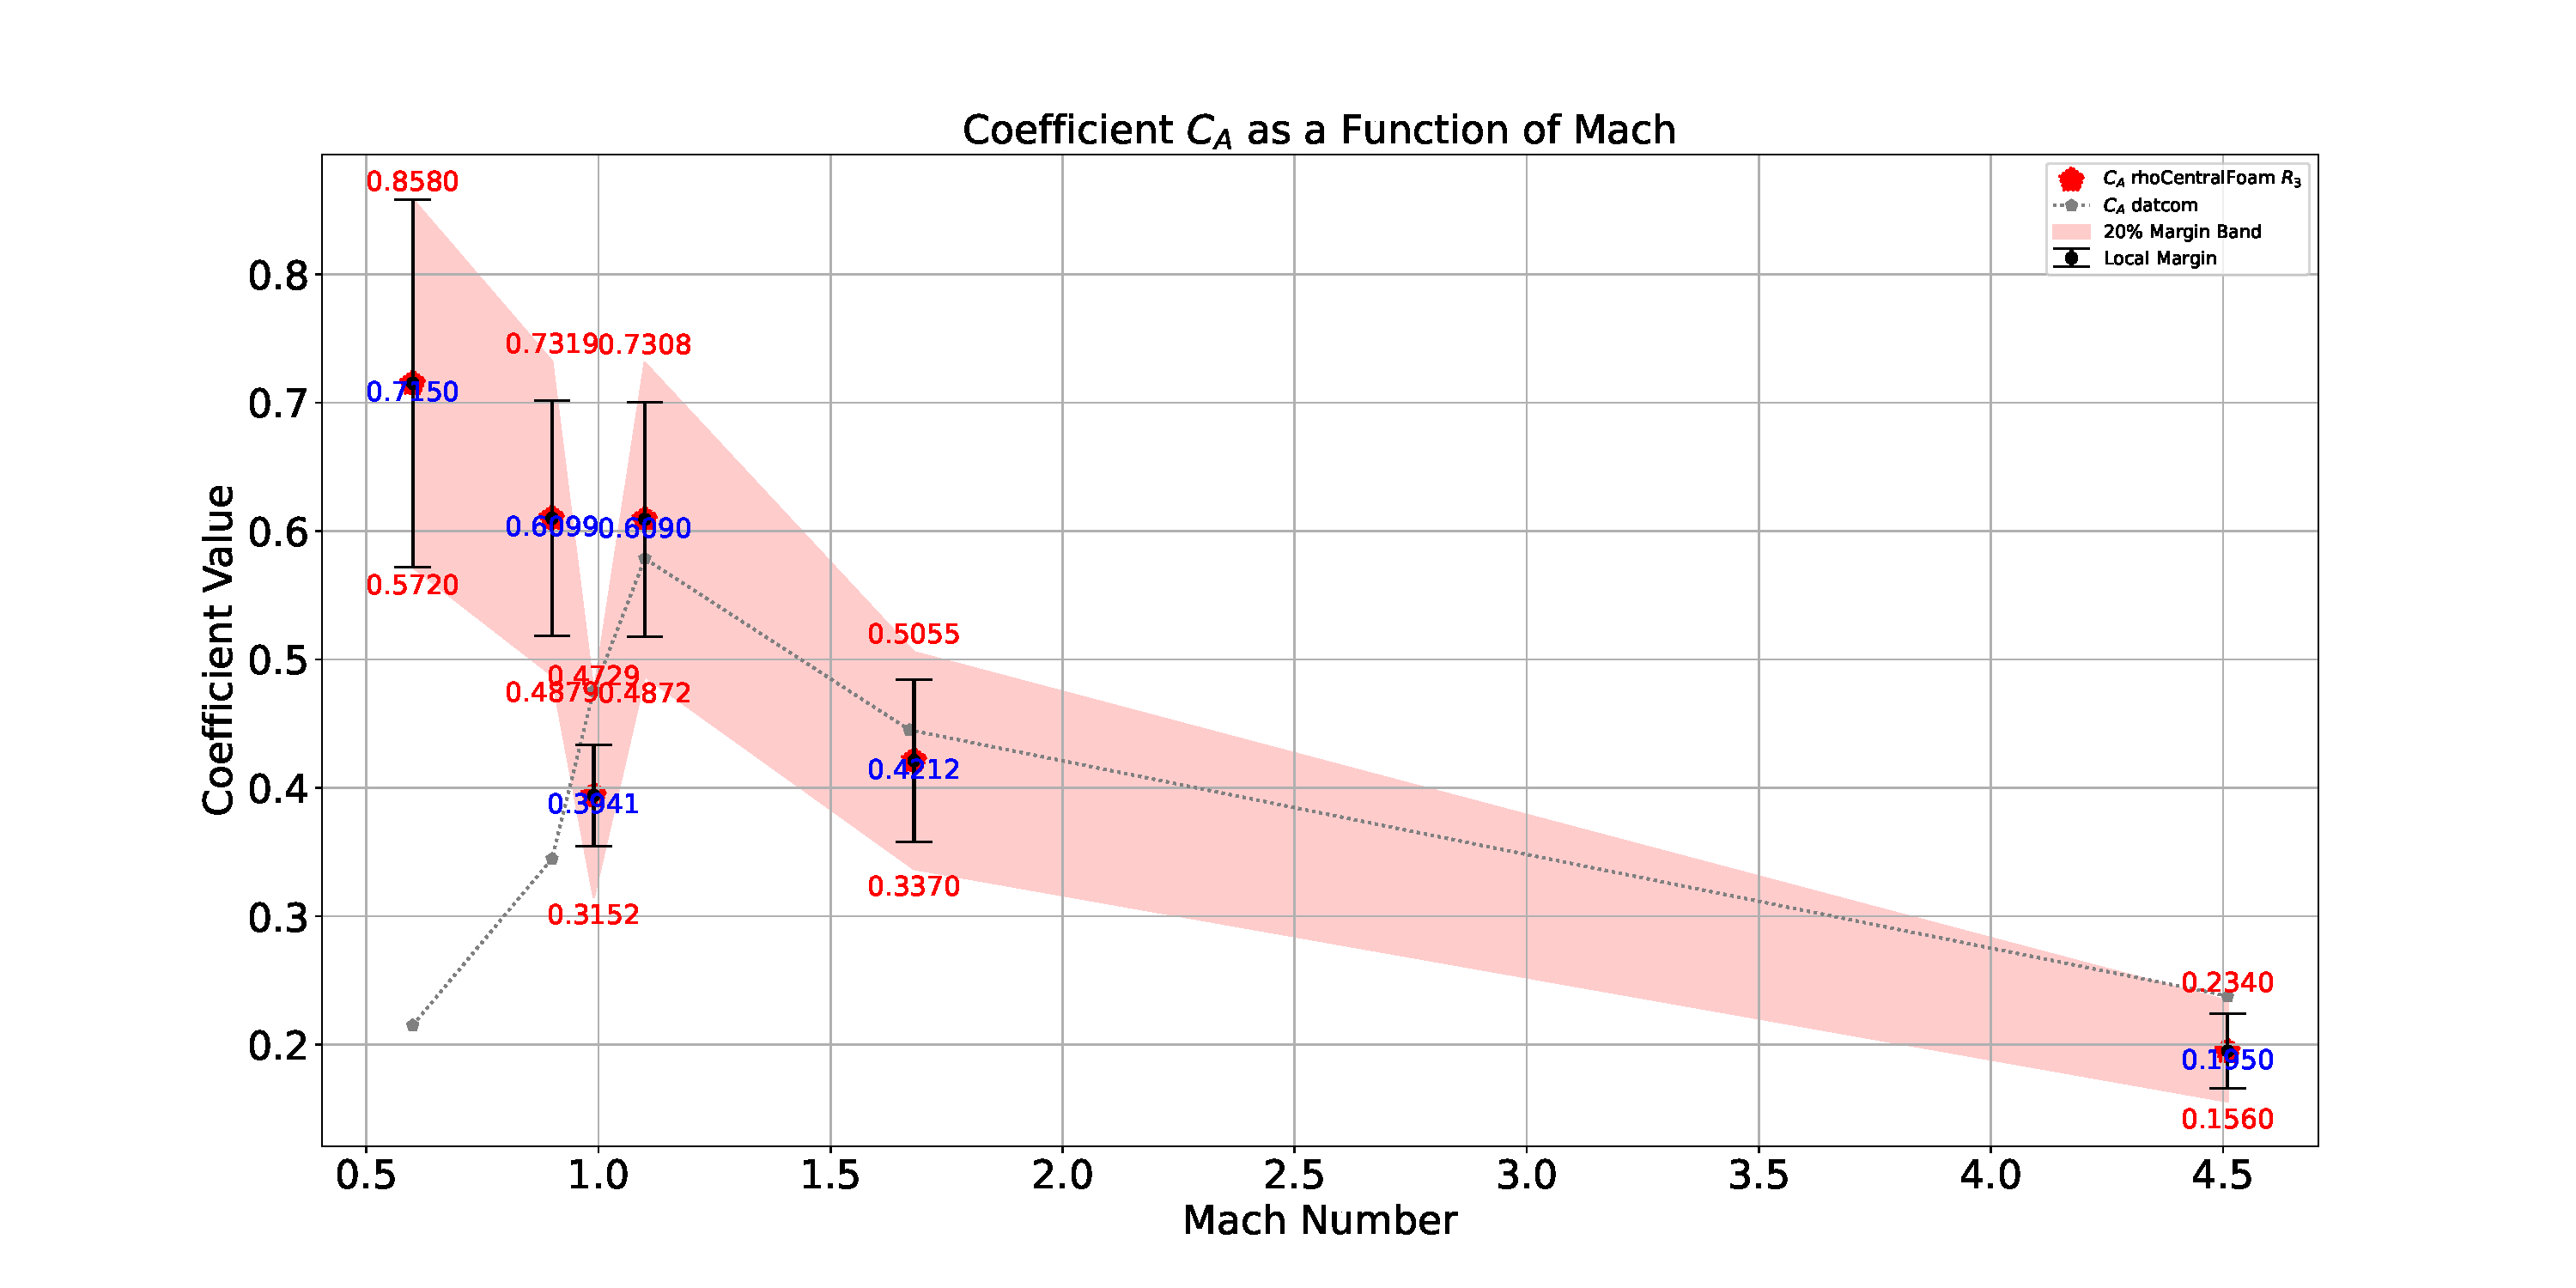
\includegraphics[width=0.995\linewidth]{figs/eris/eris4_CA.pdf}\\
%    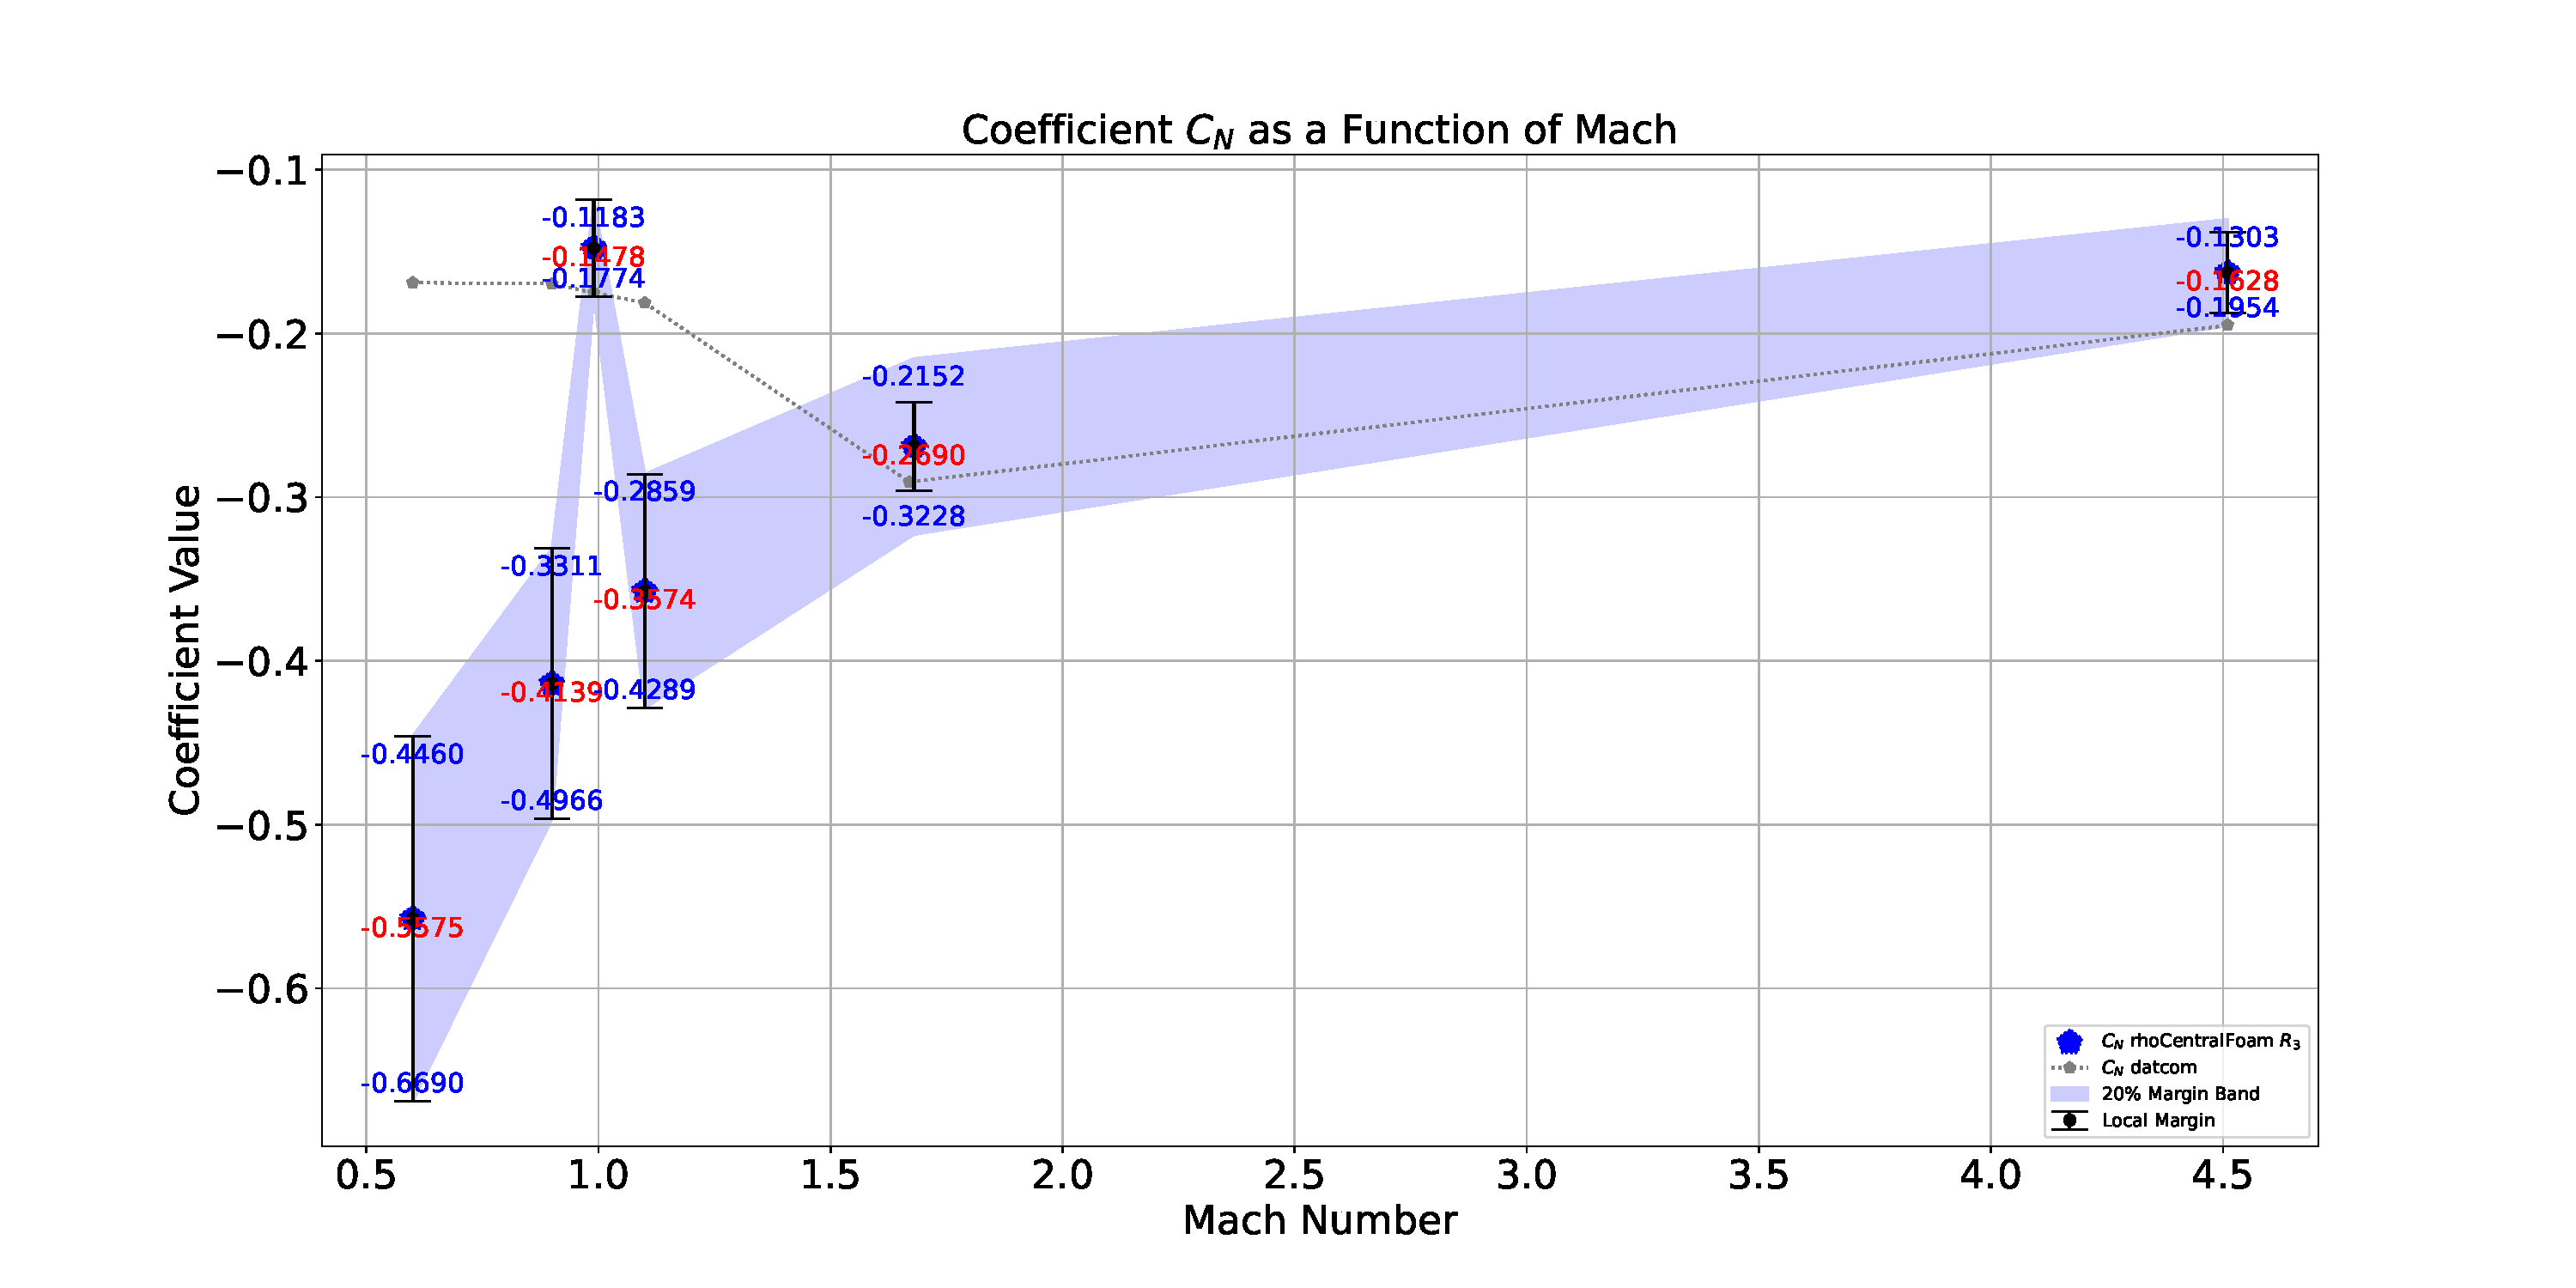
\includegraphics[width=0.995\linewidth]{figs/eris/eris4_CN.pdf}\\
%    \includegraphics[width=0.995\linewidth]{figs/eris/eris4_CM.pdf}
%    \caption{Aerodynamic coefficients, $C_A$, $C_N$, $C_M$, for the Eris Block 1.1 Rev. A configuration \textbf{S123F} launch vehicle as a function of Mach number for an angle of attach $\alpha$ = 4$^\circ$. The applied uncertainty margin was imported from the benchmark validation test case ARCAS.}
%    \label{fig:eris-CA-CA-CM_alpha4}
%\end{figure}
%
\begin{figure}[H]
    \centering
    \vspace{-0.4cm}
    \includegraphics[width=0.995\linewidth]{figs/eris/S123F/fixed/Eris4_CA.pdf}\\
    \vspace{-0.4cm}
    \includegraphics[width=0.995\linewidth]{figs/eris/S123F/fixed/Eris4_CN.pdf}\\
    \vspace{-0.4cm}
    \includegraphics[width=0.995\linewidth]{figs/eris/S123F/fixed/Eris4_CM.pdf}
    \caption{Aerodynamic coefficients, $C_A$, $C_N$, $C_M$, for the Eris Block 1.1 Rev. A configuration \textbf{S123F} launch vehicle as a function of Mach number for an angle of attack \hl{$\alpha$ = 4$^\circ$}. The applied uncertainty margin was imported from the benchmark validation test case ARCAS.}
    \label{fig:eris-CA-CA-CM_alpha4}
\end{figure}
%
\subsubsection{Ablation analysis}\label{subsubsec:ablation}
%%%%%%%%%%%%%%%%%%%%%%%%%%%%%%%%%%%%%%%%%%%%%%%%%%%%%%%%%%%
Given the surprising results obtained in the subsonic and transonic regime,
few other simulations were executed in order to shed some light. Only one time
was considered, $t$ = 34.253 $s$ and only for $\alpha$ = 0$^\circ$ as the most critical disagreement was attained in the low subsonic regime and most probably not related to the angle of attack. Through these additional tests few clarifications were obtained, specifically:

\begin{itemize}
    \item As shown in Listing~\ref{lst:testSA}, the Spalart-Allmaras (SA) turbulence model gives very similar results to the baseline $k$-$\omega$ SST when applied with the same wrong ICs. Thus, no significant impact was imputed to the turbulence model.
    \item As shown in Listing~\ref{lst:test_fix_wo}, The $k$-$\omega$ SST applied with the \textbf{fixed} ICs provides much better agreement with the DATCOM results and aligns with the physical intuition about the increasing $C_A$ through subsonic and transonic regimes. \textbf{The imposition of wrong ICs was regarded as main source of error. As a consequence of this, a fully automated extraction procedure, based on jupyter notebook, was used thereafter.} 
    \item A trivial but subtle aspect, critical for the correct estimation of the aerodynamic coefficients, is the definition of reference quantities and axis. Care should be paid when setting $A_{ref}$ and $l_{ref}$, which is different between ARCAS, ERIS and CHARON and could cause remarkable disagreement.
    \item Several meshes with different topological and layering features were evaluated providing comparable solution, thus confirming that there was \textbf{no mesh refinement impact involved}.
\end{itemize}

\paragraph{\texttt{t34.253\_alpha0\_fixed\_k\_omega}}
\begin{lstlisting}[caption=t34.253\_alpha0\_fixed\_k\_omega. Aerodynamic coefficients obtained with the the baseline $k$-$\omega$ SST model after fixing the values of turbulence fields of $k$ and $\omega$., label=lst:test_fix_wo, language=sh]
boundaryLayers

forceCoeffs forceCoeffs1 write:
    Coefficient Total       Pressure        Viscous         Internal
    Cd:         0.310676    0.0350351       0.275641        0
    Cd(f):      0.15534     0.0175217       0.137818        0
    Cd(r):      0.155336    0.0175134       0.137823        0
    Cl:         0.000615633 -5.92877e-06    0.000621561     0
    Cl(f):      0.00053626  0.000310232     0.000226028     0
    Cl(r):      7.93729e-05 -0.000316161    0.000395533     0
    CmPitch:    0.000228443 0.000313196     -8.47528e-05    0
    CmRoll:     1.74671e-06 4.17074e-06     -2.42403e-06    0
    CmYaw:      1.32232     1.30539         0.016929        0
    Cs:         -0.261769   -0.00119317     -0.260575       0
    Cs(f):      1.19144     1.3048          -0.113359       0
    Cs(r):      -1.45321    -1.30599        -0.147217       0
\end{lstlisting}

\paragraph{\texttt{t34.253\_alpha0\_SA}}
\begin{lstlisting}[caption=t34.253\_alpha0\_SA. Aerodynamic coefficients obtained with the the Spalart-Allmaras turbulence model using the old $R_0$ mesh., label=lst:testSA, language=bash]
boundaryLayers
forceCoeffs forceCoeffs1 write:
    Coefficient Total           Pressure        Viscous         Internal
    Cd:         0.68503         0.00131576      0.683714        0
    Cd(f):      0.342395        0.000537659     0.341857        0
    Cd(r):      0.342635        0.000778102     0.341857        0
    Cl:         0.000673293     -6.54948e-08    0.000673359     0
    Cl(f):      0.000678121     0.00034486      0.000333261     0
    Cl(r):      -4.82788e-06    -0.000344925    0.000340097     0
    CmPitch:    0.000341474     0.000344892     -3.41795e-06    0
    CmRoll:     -0.00012022     -0.000120221    1.44289e-09     0
    CmYaw:      -0.035054       -0.0356024      0.000548343     0
    Cs:         -0.0453298      -2.47021e-05    -0.0453051      0
    Cs(f):      -0.0577189      -0.0356147      -0.0221042      0
    Cs(r):      0.0123892       0.03559         -0.0232009      0
\end{lstlisting}
%
%\noindent \textcolor{red}{\textbf{As a consequence, it is required to re-run all simulations with fixed ICs.}}

\subsection{Stage 2 + 3 and Fairing (S23F)}\label{subsec:results_S23F}
%%%%%%%%%%%%%%%%%%%%%%%%%%%%%%%%%%%%%%%%%%%%%%%%%%%%%%%%%%%%%%%%%%%%%
This subsection reports all simulations performed for the aerodynamic characterization of ERIS Block 1.1 Rev. A for the S23F configuration without plume effect (motor-off) using \texttt{OpenFOAM}, \texttt{\st{Fluent}} and \texttt{DATCOM}. Only one point along the flight trajectory was selected corresponding to the separation time, $t \approx$ 107.682 s. \textcolor{blue}{As a result of the wrong initial condition setup, mentioned before, also these simulations were recomputed. Nevertheless, it was found that the new values are very similar to the previous ones. Thus, the old values can be considered reliable.}

\begin{table}[H]
    \centering
    \caption{Simulations performed for the aerodynamic characterization of the rocket ERIS Block 1.1 Rev. A for the S23F configuration without plume effect (motor-off) using \texttt{OpenFOAM}, \texttt{Fluent} and \texttt{DATCOM}. %\textcolor{red}{\textbf{\ul{This table contains wrong values and needs to be updated with fixed values shown in the figures below}.}}
    \textcolor{blue}{Blue values have been recomputed after fixing values.}}
    \label{tab:results_S23F}
    \resizebox{\textwidth}{!}{
    \begin{tabular}{ccccc|ccc|ccc|ccc|ccc|ccccccc}
    \hline 
    \hline 
        \multicolumn{5}{c|}{\textbf{Simulation}} & \multicolumn{3}{c|}{$y^+$} & \multicolumn{3}{c|}{\textbf{Coefficients}} & \multicolumn{3}{c|}{\textbf{Coeffs. last 50 iters.}} & \multicolumn{3}{c|}{\textbf{Timing}} & \multicolumn{7}{c}{\textbf{Residuals}}\tabularnewline
        \hline 
        \hline 
        Time [s] & \cellcolor{red}\textbf{Ma} & \cellcolor{lime}\textbf{AoA} & \cellcolor{cyan}\textbf{Mesh} & \cellcolor{pink}\textbf{Solver} & \textbf{min} & \textbf{max} & \textbf{avg} & \cellcolor{yellow}$C_A$ & \cellcolor{yellow}$C_N$ & \cellcolor{yellow}$C_{m}$ & $C_A$ & $C_N$ & $C_{m}$ & \textbf{Time [s]} & \textbf{Iters} & \textbf{Iter/sec} & \textbf{U} & $\omega$ & \textbf{p} & \textbf{V} & \textbf{k} & \textbf{e} & \textbf{W}\tabularnewline
        \hline 
        \hline 
        \rowcolor{green!10}
        %107.682 & 4.51 & 0 & $R_0$ & \texttt{rhoCentralFoam} & - & - & - & \textbf{2.666999e-01} & \textbf{1.020760e-03} & \textbf{1.108761e-02} & - & - & - & - & - & - & - & - & - & - & - & - & - \\ 
         107.682 & 4.51 & 0 & $R_0$ & \texttt{rhoCentralFoam} & - & - & - & \textbf{\textcolor{blue}{0.273967}} & \textbf{\textcolor{blue}{0.00127872}} & \textbf{\textcolor{blue}{0.0133724}} & - & - & - & - & - & - & - & - & - & - & - & - & - \\ 
        \rowcolor{green!10}
        107.682 & 4.51 & 2 & $R_0$ & \texttt{rhoCentralFoam} & - & - & - & \textbf{2.668742e-01} & \textbf{-7.174747e-02} & \textbf{-8.323319e-01} & - & - & - & - & - & - & - & - & - & - & - & - & - \\ 
        \rowcolor{green!10}
        %107.682 & 4.51 & {4} & $R_0$ & \texttt{rhoCentralFoam} & - & - & - & \textbf{2.684287e-01} & \textbf{-1.473825e-01} & \textbf{-1.702615e+00} & - & - & - & - & - & - & - & - & - & - & - & - & - \\
        107.682 & 4.51 & {4} & $R_0$ & \texttt{rhoCentralFoam} & - & - & - & \textbf{\textcolor{blue}{0.275354}} & \textbf{\textcolor{blue}{-0.156148}} & \textbf{\textcolor{blue}{-1.78769}} & - & - & - & - & - & - & - & - & - & - & - & - & - \\
        \rowcolor{green!40}
        107.682 & 4.51 & \cellcolor{lime}\textbf{0} & \cellcolor{cyan}$R_3$ & \texttt{rhoCentralFoam} & - & - & - & \textbf{} & \textbf{} & \textbf{} & - & - & - & - & - & - & - & - & - & - & - & - & - \\
        \rowcolor{green!40}
        107.682 & 4.51 & \cellcolor{lime}\textbf{2} & \cellcolor{cyan}$R_3$ & \texttt{rhoCentralFoam} & - & - & - & \textbf{} & \textbf{} & \textbf{} & - & - & - & - & - & - & - & - & - & - & - & - & - \\
        \rowcolor{green!40}
        107.682 & 4.51 & \cellcolor{lime}\textbf{4} & \cellcolor{cyan}$R_3$ & \texttt{rhoCentralFoam} & - & - & - & \textcolor{red}{\textbf{}} & \textcolor{red}{\textbf{}} & \textcolor{red}{\textbf{}} & - & - & - & - & - & - & - & - & - & - & - & - & - \\
        \rowcolor{blue!10}
        107.682 & 4.51 & 0 & $R_0$ & \texttt{rhoPimpleFoam} & - & - & - & \textbf{1.477024e-01} & \textbf{-2.900076e-04} & \textbf{-1.493174e-03} & - & - & - & - & - & - & - & - & - & - & - & - & - \\ 
        \rowcolor{blue!10}
        107.682 & 4.51 & 2 & $R_0$ & \texttt{rhoPimpleFoam} & - & - & - & \textbf{1.483413e-01} & \textbf{-5.547447e-02} & \textbf{-6.718191e-01} & - & - & - & - & - & - & - & - & - & - & - & - & - \\
        \rowcolor{blue!10}
        107.682 & 4.51 & 4 & $R_0$ & \texttt{rhoPimpleFoam} & - & - & - & \textbf{1.497123e-01} & \textbf{-1.153930e-01} & \textbf{-1.384669e+00} & - & - & - & - & - & - & - & - & - & - & - & - & - \\
        \rowcolor{blue!40}
        107.682 & 4.51 & 0 & $R_3$ & \texttt{rhoPimpleFoam} & - & - & - &  & &  & - & - & - & - & - & - & - & - & - & - & - & - & - \\
        \rowcolor{red!10}
        107.682 & 4.51 & 0 & $R_0$ & \texttt{Fluent} & - & - & - &  &  &  & - & - & - & - & - & - & - & - & - & - & - & - & - \\ 
        \rowcolor{red!40}
        107.682 & 4.51 & 0 & $R_3$ & \texttt{Fluent} & - & - & - &  &  &  & - & - & - & - & - & - & - & - & - & - & - & - & - \\ 
        \rowcolor{gray!10}
        107.682 & 4.51 & 0 & - & \texttt{DATCOM} & - & - & - & 0.2778 & 0.0 & 0.0 & - & - & - & - & - & - & - & - & - & - & - & - & - \\ 
        \rowcolor{gray!10}
        107.682 & 4.51 & 2 & - & \texttt{DATCOM} & - & - & - & 0.2781 & -0.0819 & -0.1198 & - & - & - & - & - & - & - & - & - & - & - & - & - \\ 
        \rowcolor{gray!10}
        107.682 & 4.51 & 4 & - & \texttt{DATCOM} & - & - & - & 0.2792 & -0.1882 & -0.3343 & - & - & - & - & - & - & - & - & - & - & - & - & - \\ 
        \rowcolor{gray!10}
        107.682 & 4.51 & 6 & - & \texttt{DATCOM} & - & - & - & 0.2809 & -0.3378 & -0.7167 & - & - & - & - & - & - & - & - & - & - & - & - & - \\
        \hline 
        \hline 
    \end{tabular}}
\end{table}

\begin{figure}[H]
    \centering
    \includegraphics[width=0.999\linewidth]{figs/eris/S23F/coefficients_vs_alpha.eps}\\
    %\includegraphics[width=0.999\linewidth]{figs/eris/S23F/eris_alpha.eps}
    \caption{Aerodynamic coefficients, $C_A$, $C_N$, $C_M$, for the Eris Block 1.1 Rev. A configuration \textbf{S23F} launch vehicle as a function of the angle of attach $\alpha$ = 0$^\circ$, 2$^\circ$, 4$^\circ$.}
    \label{fig:eris-CA-CA-CM_alpha4}
\end{figure}
%
\begin{figure}[H]
    \centering
    \includegraphics[width=0.33\linewidth]{figs/eris/S23F/eris_cn_alpha_with_margins_and_annotations.eps}
    \includegraphics[width=0.33\linewidth]{figs/eris/S23F/eris_cd_alpha_with_margins_and_annotations.eps}
    \includegraphics[width=0.33\linewidth]{figs/eris/S23F/eris_cm_alpha_with_margins_and_annotations.eps}
    \caption{Aerodynamic coefficients, $C_A$, $C_N$, $C_M$, for the Eris Block 1.1 Rev. A configuration \textbf{S23F} launch vehicle as a function of the angle of attack \hl{$\alpha$ = 0$^\circ$, 2$^\circ$, 4$^\circ$}. The applied 20\% uncertainty margin was imported from the benchmark validation test case ARCAS.}
    \label{fig:eris-CA-CA-CM_alpha4}
\end{figure}

\section{Protrusions effect}\label{sec:protrusions}
%%%%%%%%%%%%%%%%%%%%%%%%%%%%%%%%%%%%%%%%%%%%%%%%%%%
Protrusion effects~\cite{roncioni2017preliminary,roncioni2019aerodatabase} were modeled using \texttt{DATCOM} and previous available data. It was found that the effect of protrusions, apart from raceways which were already included in the baseline configuration, were negligible and no further CFD analysis was performed.
%\colorbox{green}{TBD}

\section{Plume effect}\label{sec:plume}
%%%%%%%%%%%%%%%%%%%%%%%%%%%%%%%%%%%%%%%
Following~\cite{brauckmann2011rocket,compton1975effects,pindzola1963jet,mehta2016skylon,gusman2011best,forbes2020trajectory}, plume effect on aerodynamic coefficients of Eris Block 1.1 Rev. A configuration should be investigated, as it may have a non-negligible effect on the aerodynamic coefficients, especially on the drag coefficient, $C_A$. In particular, the maximum dynamic pressure instant ($t$ = 61.62 $s$) on the flight trajectory was selected for this analysis varying the angle of attack. \textbf{\textcolor{red}{TODO}}

%\section{Confidence Level Evaluation}\label{sec:confidence}
%%%%%%%%%%%%%%%%%%%%%%%%%%%%%%%%%%%%%%%%%%%%%%%%%%%%%%%%%%%%
%The confidence level comprises \textbf{uncertainties} and \textbf{dispersion}, accounting for grid sensitivity, flow modeling, and the differences between CAD models and real-world conditions. Uncertainties were calculated using correlation and variance-based error propagation. This concept is applicable for both experimental and computational values. The experimental uncertainty is linked to direct measurements (balance) and the dispersion is linked to the repeatability of the same measurements and to additional dispersions due to the differences  between the model/model-settings and the real flight conditions. Analogously the numerical uncertainty is due to the grid sensitivity and flow modeling (i.e. turbulence modeling) and the dispersion concerns with the difference between CAD model/run settings and the real world. 
%%This last term is taken into account for both experiments and CFD with a suitable factor. 
%The final confidence level is a summation of the experimental contribution (balance and repeatability) and numerical contribution (grid and modeling). 
%
%The centre of pressure is a derived quantity of Pitching Moment $C_{My}$ and Normal Force $C_{N}$ and is strictly correlated to them:
%
%\paragraph{\textbf{Centre of Pressure} \( X_{cp} \) \textbf{Calculation}}:
%   \[
%   X_{cp} = -\frac{C_{My}}{C_{N}} \times L_{\text{ref}}
%   \]
%
%\paragraph{\textbf{Uncertainty for Centre of Pressure}$(U_{Xcp}$)}:
%   \[
%   U_{Xcp} = \sqrt{U_{CMy}^2 + U_{CN}^2 - 2 \times \text{Corr} \times U_{CMy} \times U_{CN}}
%   \]
%
%\paragraph{\textbf{Correlation} \( \text{Corr} \) \textbf{Calculation}}:
%   \[
%   \text{Corr} = \frac{\text{Covariance}(C_{N}, C_{My})}{\sigma_{C_N} \times \sigma_{C_{My}}}
%   \]
%
%\paragraph{\textbf{Covariance Calculation}}:
%   \[
%   \text{Covariance}(x, y) = \frac{1}{N} \sum (x_i - \overline{x}) \times (y_i - \overline{y})
%   \]
%
%\paragraph{\textbf{Variance Calculation}}:
%    \[
%    \sigma(x) = \sqrt{\text{Variance}(x)} = \sqrt{\frac{1}{N} \sum (x_i - \overline{x})^2}
%    \]
%
%\noindent A value of 0.9 is used and is based on available data of VEGA C repeatability measurements of wind tunnel. The formula is a direct consequence of the propagation error theory. The correlation is a non-dimensional value that ranges from zero (no correlation and higher value of uncertainty) to one (full correlation and lower value of uncertainty). From the above formula we can see that in the particular case of equal values of uncertainties for $C_{My}$ and $C_N$ and full correlation (corr = 1) we can have a null uncertainty for $X_{cp}$.
%
%\section{Final Aerodatabase}\label{sec:aedb}
%%%%%%%%%%%%%%%%%%%%%%%%%%%%%%%%%%%%%%%%%%%%
%The final ADB incorporates protrusion effects and includes confidence levels. Comparisons between CFD and experimental data show consistency across aerodynamic coefficients and pressure distributions.

\section{Conclusions}\label{sec:conclusions}
%%%%%%%%%%%%%%%%%%%%%%%%%%%%%%%%%%%%%%%%%%%%
The Eris Block 1.1 Rev. A AEDB was developed using CFD simulations, with a confidence level based on uncertainties provided by a previous numerical simulation campaign performed for the ARCAS validation testcase benchmark. Numerical results obtained by \texttt{OpenFOAM} were compared with those from \texttt{DATCOM} and with the previous estimation of aerodynamic coefficients. A reasonable level of agreement between all data, within the pre-defined margins of uncertainty of 20\%, was obtained for all flight regimes. Better agreement is generally achieved in supersonic and hypersonic regimes where a 10\% margin may be applied while subsonic and transonic regimes typically require higher margins, 25\% - 30\%. Slightly larger discrepancy with respect to \texttt{DATCOM} was observed for the $C_{M}^{pitch}$ coefficient which may be due to the DATCOM's sensitivity to the input geometry. The main deliverable of the present work, apart from this report and all simulations' repository, consists in a JSON files containing the aerodynamic coefficients for each configuration, \texttt{\hl{AERO\_ERIS\_1.1\_S123F.json}} and \texttt{\hl{AERO\_ERIS\_1.1\_S23F.json}}, respectively.

Future efforts may be devoted to include a broader class of solutions obtained from different solvers, specifically tailored to better represent some physical phenomenon such as shocks, base flow, separation flow with the aim of developing a deeper sensitivity of numerical parameters to those events. Fluent simulations could be included as well. In addition, a full investigation pertaining motor-on configuration should be performed.

%The AEDB provides flight-condition updated aerodynamic coefficients important for mission planning. %The ground to flight extrapolation procedure for the aerodynamic coefficients of the Eris launch vehicle has been presented. The extrapolation procedure is based upon the numerical evaluation of the trends with the Reynolds number of the aerodynamic coefficients at several Mach numbers. CFD results were used as support to the extrapolation methodology. It can be generally stated that a thorough knowledge of the flow structures around the vehicle, at both flight and wind tunnel conditions, gathered by means of global aerodynamic loads and surface pressure measurements, flow visualizations and computational predictions, is absolutely necessary. In fact, exploiting this knowledge, the comparisons between the experimental and numerical trends can be performed, and it can be confirmed whether both can be used to extrapolate the aerodynamic coefficients up to the flight conditions as they are, or some corrections are needed, that can be identified from the understanding of the causes of the differences between the two data sets. Where strong viscous/inviscid interactions at the Reynolds numbers of interest for the extrapolation procedure are found, a particular attention has to be dedicated to predict whether these phenomena are still present at the flight Reynolds number, and then do not affect the computed trends, or they change within the Reynolds range of interest, making necessary a deeper analysis of their effects. This is the case of the results of the tests performed on the Eris model in the hypersonic regime, as the separation at the boat tail, which is strongly influenced by Reynolds number changes, required a special experimental effort to allow the coefficients extrapolation to the flight conditions. %Finally, the dependence of the aerodynamic coefficients on the Reynolds number expressed as analytical function,  allows to simply evaluate the coefficients on trajectories that differ from the nominal one. 

%\newpage
%
%a\section*{Tables}
%a
%a1. \textbf{Mach Ranges for Aero Database Building}:
%a
%a\begin{itemize}
%a    \item \textbf{Sub-transonic-Supersonic Range}: M = 0.5 - 3.5 (Wind Tunnel and CFD data)
%a    \item \textbf{Hypersonic Range}: M = 3.5 - 7.0 (CFD data only)
%a\end{itemize}
%a
%a2. \textbf{CFD Test Matrix - 4-Stage and 3-Stage Baseline Configurations}:
%a
%a\begin{table}[h!]
%a\centering
%a\begin{tabular}{lccccc}
%a\toprule
%aRegime         & Mach [-] & Reynolds [-] & AoA [deg] & Nozzle [deg] \\
%a\midrule
%aSub-Transonic  & 0.50     & WT, INT      & 5         & 0           \\
%a               & 0.50     & Flight       & 0, 5, 10  & 0           \\
%a...            & ...      & ...          & ...       & ...         \\
%aHypersonic     & 5.00     & Flight       & 0, 5, 10  & 0           \\
%a               & 5.91     & Flight       & 0, 5, 10  & 0           \\
%a\bottomrule
%a\end{tabular}
%a\end{table}
%a
%a3. \textbf{CFD Test Matrix - 4-Stage Protrusion Configuration}:
%a
%a\begin{table}[h!]
%a\centering
%a\begin{tabular}{lccccc}
%a\toprule
%aRegime         & Mach [-] & Reynolds [-] & AoA [deg] & Roll [deg] & Nozzle [deg] \\
%a\midrule
%aSub-Transonic  & 0.95     & WT           & 5         & 0          & 0           \\
%aSupersonic     & 1.80     & WT           & 5         & 0          & 0           \\
%aHypersonic     & 5.00     & Flight       & 5         & 45         & 0           \\
%a\bottomrule
%a\end{tabular}
%a\end{table}
%a
%a4. \textbf{Experimental Test Matrix - 4-Stage Clean Configuration}:
%a
%a\begin{table}[h!]
%a\centering
%a\begin{tabular}{lcccccc}
%a\toprule
%aRegime         & Mach [-] & Reynolds [-] & AoA [deg] & Roll [deg] & Configuration & \# Polars \\
%a\midrule
%aSub-Transonic  & 0.50     & \(5.0 \times 10^6\) & -10 to 10 & -30, 0      & Baseline      & 2        \\
%a               & 0.95     & \(8.0 \times 10^6\) & -10 to 10 & -30 to 120  & Baseline      & 6        \\
%a\bottomrule
%a\end{tabular}
%a\end{table}
%a
%a5. \textbf{Experimental Test Matrix - 4-Stage Protrusion Configuration}:
%a
%a\begin{table}[h!]
%a\centering
%a\begin{tabular}{lcccccc}
%a\toprule
%aRegime         & Mach [-] & Reynolds [-] & AoA [deg] & Roll [deg] & Configuration & \# Polars \\
%a\midrule
%aSub-Transonic  & 0.50     & \(5.0 \times 10^6\) & -10, +10   & -75 to 135  & Protrusion    & 8        \\
%aSupersonic     & 1.80     & \(8.0 \times 10^6\) & -10 to 10  & -75 to 135  & Protrusion    & 8        \\
%a\bottomrule
%a\end{tabular}
%a\end{table}
%a
%a6. \textbf{Grid Characteristics}:
%a
%a\begin{table}[h!]
%a\centering
%a\begin{tabular}{lccc}
%a\toprule
%aConfiguration           & Levels & Cells (million) & Blocks \\
%a\midrule
%a4Stage sub-transonic    & 3      & 13.3            & 13     \\
%a4Stage hypersonic       & 3      & 4.1             & 77     \\
%a3Stage hypersonic       & 3      & 3.5             & 65     \\
%a\bottomrule
%a\end{tabular}
%a\end{table}

\vspace{\fill}
\begin{center}
    \hspace*{9cm} \LARGE \textbf{Lorenzo Campoli} \\
    \hspace*{9cm}\includegraphics[width=0.45\textwidth]{signature/signature0.png}
\end{center}
\vspace*{-1.0cm}

\newpage

%%%%%%%%%%%%%%%%%%%%%%%%%%%%%%%%%%%%%%%%%%%%%%%%
\bibliography{refs/refs}
\bibliographystyle{unsrt}
\addcontentsline{toc}{section}{References}
%%%%%%%%%%%%%%%%%%%%%%%%%%%%%%%%%%%%%%%%%%%%%%%%

%%%%%%%%%%%%%%%%%%%%%%%%%%%%%%%%%%%%%%%%%%%%%%%%
\appendix
\addcontentsline{toc}{section}{Appendix}
%%%%%%%%%%%%%%%%%%%%%%%%%%%%%%%%a%%%%%%%%%%%%%%%%

\newpage

\section*{Vega AEDB overview}\label{sec:vega}
%%%%%%%%%%%%%%%%%%%%%%%%%%%%%%%%%%%%%%%%%%%%%%%%
As point of curiosity, here below, some published results from the Vega launcher vehicle are reported from~\cite{roncioni2017preliminary,roncioni2019aerodatabase,roncioni2023aerodynamic,roncioni2024aerodatabase}.

\begin{figure}[H]
    \centering
    \includegraphics[width=0.95\linewidth]{figs/VEGA-ADB.png}
    %\caption{}
    \label{fig:vega-adb}
\end{figure}

\begin{figure}[H]
    \centering
    %\includegraphics[width=0.95\linewidth]{figs/fig12-vega.png}
    %\includegraphics[width=0.95\linewidth]{figs/fig13-vega.png}
    %\includegraphics[width=0.95\linewidth]{figs/fig17-vega.png}
    \includegraphics[width=0.95\linewidth]{figs/fig8-vega.png}
    \includegraphics[width=0.95\linewidth]{figs/fig7-vega.png}
    \includegraphics[width=0.95\linewidth]{figs/fig5-vega.png}
    %\caption{}
    \label{fig:vega-adb}
\end{figure}

\begin{figure}[H]
    \centering
    \includegraphics[width=0.95\linewidth]{figs/fig12-vega.png}
    \includegraphics[width=0.95\linewidth]{figs/fig13-vega.png}
    %\includegraphics[width=0.95\linewidth]{figs/fig17-vega.png}
    %\includegraphics[width=0.95\linewidth]{figs/fig5-vega.png}
    %\includegraphics[width=0.95\linewidth]{figs/fig8-vega.png}
    %\includegraphics[width=0.95\linewidth]{figs/fig7-vega.png}
    %\caption{}
    \label{fig:vega-adb}
\end{figure}

\newpage % TODO
%\section{Work in Progress}

\begin{description}
    \item[Checklists] Checklists to go through during peer review of the analysis.
\end{description}

\subsection*{Pre-setup Checks}
\begin{itemize}
    \item[$\checkmark$] Goals of the analysis defined. [\textbf{Sect}.~\ref{sec:intro}]
    \item[$\checkmark$] All operating cases and conditions identified, both flight and ground if applicable. [\textbf{Sect}.~\ref{sec:description}]
    \item[$\checkmark$] Boundary and initial conditions identified and selected.
    \item[$\checkmark$] Required dimensionality of the spatial model understood (2D, full 3D, slice 3D).
    \item[$\checkmark$] Appropriate temporal modelling identified (steady or transient).
    \item[$\checkmark$] Made educated guess of what final results will look like.
    \item[$\checkmark$] Assumptions being made have been identified.
    \item[$\checkmark$] Remember that CFD should stand for Computational Fluid Dynamics and not Colours For Director!
\end{itemize}

\subsection*{Setup Checks}

\subsubsection*{Geometry and Mesh:}
\begin{itemize}
    \item[$\checkmark$] Geometry is at worst case tolerances.
    \item[$\checkmark$] Check the geometry is a watertight 3D solid or 2D surface.
    \item[$\checkmark$] Use descriptive strings to name entities (e.g. fluid, inlet, outlet, wall, axis, symmetry, periodicity).
    \item[$\checkmark$] If using a 2D axisymmetric model, check the axis of rotation is the x-axis of the model.
    \item[$\checkmark$] Choose suitable mesh type for low vs large cell count and simple vs complex geometries.
    \item[$\checkmark$] Select appropriate meshing methods, global controls, and local sizings.
    \item[$\checkmark$] If resolving directly the wall boundary layer is important, use inflation layers to achieve y+ ~ 1 (Fluent 2023 R2 Theory Guide 4.7.3).
    \item[$\checkmark$] If using wall functions, use inflation layers to achieve a y+ of an appropriate range for the specified near-wall treatment setting (Fluent 2023 R2 Theory Guide 4.17).
    \item[$\checkmark$] Assure a constant growth rate between inflation layers and volume mesh.
    \item[$\checkmark$] Check that in the regions of interest the mesh does not have high growth rate or large steps in mesh size such as octree transitions in hex mesh.
    \item[$\checkmark$] Check mesh quality metrics (e.g. orthogonal quality > 0.1, average skewness < 0.33, maximum skewness < 0.85) (Fluent 2023 R2 User's Guide II.5.3 and III.6.2).
    \item[$\checkmark$] Mesh passes fluent mesh check.
\end{itemize}

\subsubsection*{Physics Models and Boundary Conditions:}
\begin{itemize}
    \item[$\checkmark$] Select the suitable physics models.
    \item[$\checkmark$] Use the appropriate turbulence model (k-w SST industry standard for several problems). Consider activating curvature correction for swirling flows.
    \item[$\checkmark$] Double check material properties.
    \item[$\checkmark$] Ideal or real fluid properties properly defined and sources documented for new properties entered.
    \item[$\checkmark$] Correct units used for all boundary condition inputs.
    \item[$\checkmark$] Reference quantities set appropriately.
    \item[$\checkmark$] Operating pressure set appropriately to avoid roundoff error problems (Fluent 2023 R2 User's Guide III.8.14). Where no pressure boundary conditions are used, reference pressure location has been set (Fluent 2023 R2 User's Guide III.8.15).
    \item[$\checkmark$] Pressures are all input as gauge wrt the operating pressure.
    \item[$\checkmark$] Gravity set correctly if needed.
\end{itemize}

\subsubsection*{Numerical Methods and Solution Controls:}
\begin{itemize}
    \item[$\checkmark$] Considered if the single or double precision solver is needed (Fluent User's Guide I.4.1.2.2).
    \item[$\checkmark$] Choose the appropriate solver type and temporal model.
    \item[$\checkmark$] Use 2nd order schemes if possible.
    \item[$\checkmark$] Adjust absolute convergence criteria for residuals (e.g. to 1E-6).
    \item[$\checkmark$] Define suitable report definitions and monitors.
    \item[$\checkmark$] Autosave data file every XXX iterations to preserve results and retain only the most recent files.
\end{itemize}

\subsection*{Results}
\begin{longtable}{|c|c|c|}
    \hline
    Case & Key result 1 & Key result 2 \\
    \hline
    \endfirsthead
    \hline
    Case & Key result 1 & Key result 2 \\
    \hline
    \endhead
    \hline
    \endfoot
    \hline
    Case 1 & Value 1 & Value 2 \\
    Case 2 & Value 1 & Value 2 \\
\end{longtable}

\noindent Concise presentation of findings with screenshots only of crucial parts.

\noindent Comparison to analytical methods or sanity checks.

\noindent Add table of sensitivity to assumptions if applicable.

\subsection*{Mesh Independence Check}
\begin{longtable}{|c|c|c|c|}
    \hline
    Case & \# of elements & Change in key result 1 & Change in key result 2 \\
    \hline
    \endfirsthead
    \hline
    Case & \# of elements & Change in key result 1 & Change in key result 2 \\
    \hline
    \endhead
    \hline
    \endfoot
    \hline
    Case 1 & 1000 & 0.01 & 0.02 \\
    Case 2 & 2000 & 0.005 & 0.01 \\
\end{longtable}

\newpage

\section*{Goals}
\begin{itemize}
    \item \textbf{What are you analysing (and which locations are important)?}
    \item \textbf{Why are you doing it (Pressure losses estimate, prior to manufacture, trade study)?}
    \item \textbf{How much accuracy is needed?}
    \item \textbf{Does this need CFD or could it be done with analytical methods, or testing?}
\end{itemize}

\section*{Geometry and Mesh}
\begin{itemize}
    \item \textbf{Screenshot of geometry.}
    \item \textbf{Screenshot of typical mesh and refined regions.}
    \item \textbf{Key mesh sizing.}
    \item \textbf{Overall mesh quality.}
    \item \textbf{Total number of elements.}
\end{itemize}

\section*{Physics Model and Boundary Conditions}
\begin{itemize}
    \item \textbf{Include annotated screenshots as required.}
\end{itemize}

\section*{Numerical Methods and Solution Controls}
\begin{itemize}
    \item \textbf{Solver settings details screenshot.}
\end{itemize}

\section*{Work in Progress}

\begin{description}
    \item[Checklists] Checklists to go through during peer review of the analysis.
\end{description}

\subsection*{Pre-setup Checks}
\begin{itemize}
    \item[$\checkmark$] Goals of the analysis defined. [\textbf{Sect}.~\ref{sec:intro}]
    \item[$\checkmark$] All operating cases and conditions identified, both flight and ground if applicable. [\textbf{Sect}.~\ref{sec:description}]
    \item[$\checkmark$] Boundary and initial conditions identified and selected. [\textbf{This is documented in the Subsection about "Boundary Condition Types" and "Boundary Condition Types for Walls" in the ARCAS report, as they are exactly the same in Eris.}]
    \item[X] Required dimensionality of the spatial model understood (2D, full 3D, slice 3D).
    \item[$\checkmark$] Appropriate temporal modelling identified (steady or transient).
    [\textbf{This is documented in the Subsection about "Time Scheme - Euler vs. localEuler" in the ARCAS report, as they are exactly the same in Eris.}]
    \item[X] Made educated guess of what final results will look like.
    \item[X] Assumptions being made have been identified.
    \item[$\checkmark$] Remember that CFD should stand for Computational Fluid Dynamics and not Colours For Director!
\end{itemize}

\subsection*{Setup Checks}
%%%%%%%%%%%%%%%%%%%%%%%%%%

\subsubsection*{Geometry and Mesh:}
%%%%%%%%%%%%%%%%%%%%%%%%%%%%%%%%%%%
\begin{itemize}
    \item[] Geometry is at worst case tolerances.
    \item[$\checkmark$] Check the geometry is a watertight 3D solid or 2D surface.
    \textbf{The geometry was extracted from the original CAD as .stl file. No other manipulations were performed.}
    \item[$\checkmark$] Use descriptive strings to name entities (e.g. fluid, inlet, outlet, wall, axis, symmetry, periodicity). [\textbf{This is documented in the Subsection about "Boundary Condition Types" in the ARCAS report, as they are exactly the same in Eris.}]
    \item[$\checkmark$] If using a 2D axisymmetric model, check the axis of rotation is the x-axis of the model. \textbf{This is confirmed.}
    \item[$\checkmark$] Choose suitable mesh type for low vs large cell count and simple vs complex geometries. \textbf{A cartesian structured mesh was adopted as it provides the highest accuracy at the lowest computational cost, (highest efficiency).}
    \item[$\checkmark$] Select appropriate meshing methods, global controls, and local sizings.
    \textbf{The mesh features are controlled by several quality metrics, as defined in \href{https://www.openfoam.com/documentation/guides/latest/doc/guide-meshing-snappyhexmesh-meshquality.html}{this guide} and \href{https://www.wolfdynamics.com/tutorials.html?id=177}{this tutorial}, for SnappyHexMEsh and CfMesh meshing tools, respectively. In both cases, a \texttt{meshQualityDictionary} file is defined in /system/ folder in each testcase directory and used to monitor the quality of the generated mesh.}
    \item[$\checkmark$] If resolving directly the wall boundary layer is important, use inflation layers to achieve y+ ~ 1 (Fluent 2023 R2 Theory Guide 4.7.3).
    \textbf{Inflation layering was evaluated and adopted values in the range 1.1 - 1.4 for finer to coarser meshes, respectively. Nevertheless, it was found that due to the fact that wall functions were used for all turbulence parameters, boundary layer effects were limited.}
    \item[$\checkmark$] If using wall functions, use inflation layers to achieve a y+ of an appropriate range for the specified near-wall treatment setting (Fluent 2023 R2 Theory Guide 4.17). \textbf{This is confirmed.}
    \item[X] Assure a constant growth rate between inflation layers and volume mesh.
    \item[$\checkmark$] Check that in the regions of interest the mesh does not have high growth rate or large steps in mesh size such as octree transitions in hex mesh. \textbf{This is partially confirmed. Improved refinement may be advisable in the wake region.}
    \item[$\checkmark$] Check mesh quality metrics (e.g. orthogonal quality > 0.1, average skewness < 0.33, maximum skewness < 0.85) (Fluent 2023 R2 User's Guide II.5.3 and III.6.2).
    \textbf{According to the mesh quality values defined in the \texttt{meshQualityDictionary} file, this is confirmed.}
    \item[$\checkmark$] Mesh passes fluent mesh check. \textbf{Mesh passes OpenFOAM mesh check, or with minor fails, non-impacting the solution as proved in the ablation analysis in Subsect.~\ref{subsubsec:ablation}.} 
\end{itemize}

\subsubsection*{Physics Models and Boundary Conditions:}
%%%%%%%%%%%%%%%%%%%%%%%%%%%%%%%%%%%%%%%%%%%%%%%%%%%%%%%%
\begin{itemize}
    \item[$\checkmark$] Select the suitable physics models.
    \textbf{A discussion about the choice of the \texttt{OpenFOAM} numerical solver was reported in the "Selected Solvers" section of the ARCAS report, highlighting the strength and weaknesses of each solver. In general terms, they correspond to the density-based (DB) and pressure-based (PD) \texttt{Fluent} solvers. Further info can be found at \href{https://www.openfoam.com/documentation/guides/latest/doc/guide-applications-solvers-compressible-rhoCentralFoam.html}{rhoCentralFoam} and \href{https://www.openfoam.com/documentation/guides/latest/doc/guide-applications-solvers-compressible-rhoPimpleFoam.html}{rhoPimpleFoam}.}
    \item[$\checkmark$] Use the appropriate turbulence model (k-w SST industry standard for several problems). Consider activating curvature correction for swirling flows.
    \textbf{The $k$-$\omega$ SST turbulence model was adopted as baseline. Other models were also investigated such as Spalart-Allmaras, $k$-$\epsilon$ without significant differences in the results. The ARCAS testcase was also validated on the $k$-$\omega$ SST model.}
    \item[$\checkmark$] Double check material properties.
    \item[$\checkmark$] Ideal or real fluid properties properly defined and sources documented for new properties entered. 
    \textbf{Fluid/material properties are defined in the folder file \texttt{/constant/}\textit{thermophysicalProperties} file, reproduced below. These are the default for \texttt{OpenFOAM} and they were not modified. They are equivalent to the fluid/material definition of \texttt{Fluent}.}
    \begin{lstlisting}
thermoType
{
    type            hePsiThermo;
    mixture         pureMixture;
    transport       sutherland;
    thermo          hConst;
    equationOfState perfectGas;
    specie          specie;
    energy          sensibleInternalEnergy;
}

mixture
{
    specie
    {
        molWeight       28.01348;
    }
    thermodynamics
    {
        Cp              1004.4;
        Hf              0;
    }
    transport
    {
        As              1.458e-06;
        Ts              110;
        Pr              0.72;
    }
}
    \end{lstlisting}
    \item[$\checkmark$] Correct units used for all boundary condition inputs.
    \item[$\checkmark$] Reference quantities set appropriately.
    \textbf{This is critical for the correct evaluation of the aerodynamic coefficients. Several times they were set wrongly, and finally an automatic procedure based on bash scripting was put in place to bypass any issue in these regards.}
    \item[X] Operating pressure set appropriately to avoid roundoff error problems (Fluent 2023 R2 User's Guide III.8.14). Where no pressure boundary conditions are used, reference pressure location has been set (Fluent 2023 R2 User's Guide III.8.15).
    \item[$\checkmark$] Pressures are all input as gauge w.r.t. the operating pressure.
    \textbf{An equivalent gauge (effective free-stream) pressure was automatically extracted from flight trajectory file and imposed.}
    \item[X] Gravity set correctly if needed.
\end{itemize}

\subsubsection*{Numerical Methods and Solution Controls:}
\begin{itemize}
\item[$\checkmark$] Considered if the single or double precision solver is needed (Fluent User's Guide I.4.1.2.2). \textbf{Double precision only.}
    \item[$\checkmark$] Choose the appropriate solver type and temporal model. \textbf{Already commented about this in previous point (Subsection about "Time Scheme - Euler vs. localEuler" in the ARCAS report, as they are exactly the same in Eris).}
    \item[$\checkmark$] Use 2nd order schemes if possible. \textbf{Numerical strategy adopted was detailed in the "Execution Strategy" subsection of the ARCAS report.}
    \item[$\checkmark$] Adjust absolute convergence criteria for residuals (e.g. to 1E-6).
    \textbf{Several convergence criteria were used as detailed in the "Execution Strategy" subsection of the ARCAS report.}
    \item[$\checkmark$] Define suitable report definitions and monitors. \textbf{ Several parameters were monitored as detailed in the "Execution Strategy" subsection of the ARCAS report. Basically, the standard macrovariables and $C_A$, $C_N$ and $C_M$.} An assumed converged trend of the aerodynamic coefficients is shown in Figure~\ref{fig:aero-conv}. \textbf{It should be noticed that not in all cases we obtain such a smooth profile, especially around transonic regime were wiggles could remain or in the case of a CFL too close to the stability value. In this case, an average value was calculated weighted on the last 100 iterations.}
    \begin{figure}[H]
        \centering
        \includegraphics[width=0.95\linewidth]{figs/eris/S123F/aero_conv.png}
        \caption{A typical trend of assumed converged aerodynamic coefficients.}
        \label{fig:aero-conv}
    \end{figure}
    \item[$\checkmark$] Autosave data file every XXX iterations to preserve results and retain only the most recent files. \textbf{Solutions are saved each 50 iteration and retaining only the last two solutions.}
\end{itemize}

\subsection*{Results}
\begin{longtable}{|c|c|c|}
    \hline
    Case & Key result 1 & Key result 2 \\
    \hline
    \endfirsthead
    \hline
    Case & Key result 1 & Key result 2 \\
    \hline
    \endhead
    \hline
    \endfoot
    \hline
    Case 1 & Value 1 & Value 2 \\
    Case 2 & Value 1 & Value 2 \\
\end{longtable}

\noindent Concise presentation of findings with screenshots only of crucial parts.

\noindent Comparison to analytical methods or sanity checks.

\noindent Add table of sensitivity to assumptions if applicable.

\subsection*{Mesh Independence Check}
\begin{longtable}{|c|c|c|c|}
    \hline
    Case & \# of elements & Change in key result 1 & Change in key result 2 \\
    \hline
    \endfirsthead
    \hline
    Case & \# of elements & Change in key result 1 & Change in key result 2 \\
    \hline
    \endhead
    \hline
    \endfoot
    \hline
    Case 1 & 1000 & 0.01 & 0.02 \\
    Case 2 & 2000 & 0.005 & 0.01 \\
\end{longtable}

\section*{Goals}
\begin{itemize}
    \item \textbf{What are you analysing (and which locations are important)?}
    \textcolor{green}{We want to generate aerodynamic coefficients for Eris 1.1 Rev. A LV configuration S123F and S23F.}
    \item \textbf{Why are you doing it (Pressure losses estimate, prior to manufacture, trade study)?} \textcolor{green}{We want to compare CFD results with old estimates and DATCOM predictions. Moreover, we want to reduce the uncertainty margins.}
    \item \textbf{How much accuracy is needed?}
    \textcolor{green}{Simulation were started in 1st order and concluded in second order.}
    \item \textbf{Does this need CFD or could it be done with analytical methods, or testing?}
    \textcolor{green}{It turns out that DATCOM results are very valuable and in good agreement with CFD solutions.}
\end{itemize}

\section*{Geometry and Mesh}
\begin{itemize}
    \item \textbf{Screenshot of geometry.} $\checkmark$
    \item \textbf{Screenshot of typical mesh and refined regions.} $\checkmark$
    \item \textbf{Key mesh sizing.} $\checkmark$
    \item \textbf{Overall mesh quality.} $\checkmark$
    \item \textbf{Total number of elements.} $\checkmark$
\end{itemize}

\section*{Physics Model and Boundary Conditions}
\begin{itemize}
    \item \textbf{Include annotated screenshots as required.}
\end{itemize}

\section*{Numerical Methods and Solution Controls}
\begin{itemize}
    \item \textbf{Solver settings details screenshot.} 
\end{itemize}

\noindent \textcolor{blue}{* I would argue that screenshots are not really a reproducible source of information, easy to become obsolete if not symbolically linked and automatically updated at each review (CD/CI fashion or similar).}

\vspace{0.5cm}

\noindent \textcolor{magenta}{** At the moment the directory tree is automatically generated and populate through script templating with a medium level of flexibility.}

\newpage

\section*{Grid convergence analysis}
In this appendix, I report the Python script used to perform grid convergence analysis implemented from \href{https://cfd.university/blog/how-to-manage-uncertainty-in-cfd-the-grid-convergence-index}{this link}.

\begin{lstlisting}[language=Python, caption=Python script used to perform grid convergence analysis., label=lst:gca]
import numpy as np

class GridConvergenceStudy:
    def __init__(self, phi_fine, phi_medium, phi_coarse, cells_fine, cells_medium, cells_coarse):
        self.phi1 = phi_fine    # Fine grid solution
        self.phi2 = phi_medium  # Medium grid solution
        self.phi3 = phi_coarse  # Coarse grid solution
        self.N1 = cells_fine    # Fine grid cell count
        self.N2 = cells_medium  # Medium grid cell count
        self.N3 = cells_coarse  # Coarse grid cell count

    @staticmethod
    def representative_spacing(cell_sizes, dimension):
        """Calculate the representative grid spacing."""
        h = np.mean(np.array(cell_sizes) ** (1 / dimension))
        return h

    def calculate_refinement_ratios(self):
        """Calculate r21 (medium-to-fine) and r32 (coarse-to-medium) refinement ratios."""
        h1 = self.representative_spacing(self.N1, 3)
        h2 = self.representative_spacing(self.N2, 3)
        h3 = self.representative_spacing(self.N3, 3)
        r21 = h1 / h2
        r32 = h2 / h3
       return r21, r32

    def observed_order_of_approximation(self, r21, r32):
        """Calculate the observed order of convergence iteratively."""
        eps = 1
        iteration = 0
        max_iterations = 100
        p = 2  # Initial guess
        e21 = self.phi1 - self.phi2
        e32 = self.phi2 - self.phi3

        while eps > 1e-6 and iteration < max_iterations:
            p_old = p
            s = np.sign(e32 / e21)
            q = np.log((r21 ** p - s) / (r32 ** p - s))
            p = (1.0 / np.log(r21)) * (abs(np.log(abs(e32 / e21))) + abs(q))
            eps = abs((p - p_old) / p_old)
            iteration += 1

        if iteration == max_iterations:
            print("WARNING: Maximum iterations reached while calculating observed order.")
        return p

    def convergence_condition(self):
        """Calculate the convergence condition."""
        CR = (self.phi3 - self.phi2) / (self.phi2 - self.phi1)
        if CR < -1:
            return "Oscillatory divergence"
        elif -1 <= CR < 0:
            return "Oscillatory convergence"
        elif 0 <= CR < 1:
            return "Monotonic convergence"
        else:
            return "Monotonic divergence"

    def richardson_extrapolation(self, r21, p):
        """Calculate Richardson extrapolated value."""
        return (r21 ** p * self.phi1 - self.phi2) / (r21 ** p - 1)

    def errors_and_gci(self, r21, r32, p):
        """Calculate errors and Grid Convergence Index (GCI)."""
        e21 = abs((self.phi1 - self.phi2) / self.phi1)
        e32 = abs((self.phi2 - self.phi3) / self.phi2)
        GCI21 = 1.25 * e21 / (r21 ** p - 1)
        GCI32 = 1.25 * e32 / (r32 ** p - 1)
        return e21, e32, GCI21, GCI32

    def asymptotic_range(self, GCI21, GCI32, r21, p):
        """Calculate the asymptotic range."""
        return r21 ** p * GCI32 / GCI21

    def optimal_grid_refinement(self, GCI_target, GCI21, p):
        """Estimate the optimal grid refinement ratio."""
        return (GCI21 / GCI_target) ** (1 / p)

    def save_results(self, filename):
        """Save results to file."""
        with open(filename, 'w') as file:
            for line in self.results:
                file.write(line + "\n")
        print(f"Results saved to {filename}")

# Example usage

# Example solutions on fine, medium, coarse grids
# Choose the desired variable upon which perform the 
# grid convergence analysis, for pressure or velocity
phi1, phi2, phi3 = 0.1, 0.12, 0.15 

# Example grid sizes
N1, N2, N3 = 1.6e6, 4e5, 1e5

study = GridConvergenceStudy(phi1, phi2, phi3, N1, N2, N3)

# Step 1: Refinement ratios
r21, r32 = study.calculate_refinement_ratios()

# Step 2: Observed order of approximation
p = study.observed_order_of_approximation(r21, r32)

# Step 3: Convergence condition
convergence = study.convergence_condition()

# Step 4: Richardson extrapolated value
phi_extrapolated = study.richardson_extrapolation(r21, p)

# Step 5: Errors and GCIs
e21, e32, GCI21, GCI32 = study.errors_and_gci(r21, r32, p)

# Step 6: Asymptotic range
AR = study.asymptotic_range(GCI21, GCI32, r21, p)

# Step 7: Optimal grid refinement
optimal_r = study.optimal_grid_refinement(0.05, GCI21, p)

# Output results
print(f"Refinement Ratios: r21={r21}, r32={r32}")
print(f"Observed Order of Approximation: p={p}")
print(f"Convergence Condition: {convergence}")
print(f"Richardson Extrapolated Value: {phi_extrapolated}")
print(f"Errors: e21={e21}, e32={e32}")
print(f"Grid Convergence Index: GCI21={GCI21}, GCI32={GCI32}")
print(f"Asymptotic Range: AR={AR}")
print(f"Optimal Refinement Ratio for Target GCI: {optimal_r}")
\end{lstlisting}

\newpage

\section*{Post-processing script}
%%%%%%%%%%%%%%%%%%%%%%%%%%%%%%%%
In this appendix I report the Python script used to post-process all the available solutions.
This script processes only the S123F configuration but an identical one, with appropriate minimal changes, was used for the S23F configuration. It is not elegant coding style but it gives an idea of the workflow and the relative position of data.
%
\begin{lstlisting}[language=Python, caption=Python script used to post-process numerical solutions. To report bugs email to: lorenzo.campoli@gspace.com, label=lst:pp]
#!/usr/bin/env python
# coding: utf-8

# # Eris Block 1.1 Rev. A Configuration S123F -- Aerodynamic Coefficients
#
# Storing of integrated values from OpenFOAM simulation in rhoCentralFoam:
# 
# - total pitch moment coefficient: Cm
# - total drag coefficient: Cd
# - total lift coefficient: Cl
# 
# | Coefficient | Description                            |
# |-------------|----------------------------------------|
# | Cd          | Drag coefficient                       |
# | Cs          | Side-force coefficient                 |
# | Cl          | Lift coefficient                       |
# | CmRoll      | Roll-moment coefficient                |
# | CmPitch     | Pitch-moment coefficient               |
# | CmYaw       | Yaw-moment coefficient                 |
# | Cdf         | Front-axle drag coefficient            |
# | Csf         | Front-axle side-force coefficient      |
# | Clf         | Front-axle lift coefficient            |
# | Cdr         | Rear-axle drag coefficient             |
# | Csr         | Rear-axle side-force coefficient       |
# | Clr         | Rear-axle lift coefficient             |
# 
# The force coefficients can also be optionally output in terms of their front and rear axle constituents:
# 
#     Cd{f,r} = 0.5*Cd {+,-} CmRoll
#     Cs{f,r} = 0.5*Cs {+,-} CmYaw
#     Cl{f,r} = 0.5*Cl {+,-} CmPitch
# 
#  where f and r represent front and rear axles, respectively.
# 
# Force and moment coefficients are output in their total and constituent components:
# 
#     total force and moment coefficients
#     pressure contributions
#     viscous contributions
#     porous resistance contributions (optional)
# 
# Force and moment coefficients can be computed and output in:
# 
#     the global Cartesian coordinate system (default)
#     a user-defined Cartesian coordinate system
# 
# Forces comprise normal pressure:
# 
# $$
# F_p = \sum_i \rho_i \, \mathbf{s}_{f,i} \, (p_i - p_{\text{ref}})
# $$
# 
# and tangential viscous contributions:
# 
# $$
# F_v = \sum_i \mathbf{s}_{f,i} \cdot (\mu \mathbf{R}_{\text{dev}})
# $$
# 
# Where:
# - $\rho$ is the density,
# - $\mathbf{s}_{f,i}$ is the face area vector,
# - $p$ is the pressure,
# - $\mu$ is the dynamic viscosity,
# - $\mathbf{R}_{\text{dev}}$ is the deviatoric stress tensor.
# 
# https://www.openfoam.com/documentation/guides/latest/api/classFoam_1_1functionObjects_1_1forceCoeffs.html#details

import json
import matplotlib
import matplotlib.pyplot as plt
import numpy as np
import os
import pandas as pd
import subprocess
import sys
import warnings

plt.rcParams.update({'font.size': 22})
warnings.filterwarnings('ignore')

# Get the current working directory
current_path = os.getcwd()
print(f"Current path saved: {current_path}")

# # Load old AERO results

# Path to the JSON file
file_path = "./Eris_B1_1_Aerodynamics.json"

# Load the JSON data
with open(file_path, 'r') as file:
    data = json.load(file)

# Access the main sections
aerodynamics_data = data.get("Aerodynamics", {})

# Accessing specific phases
phase_123F = aerodynamics_data.get("Phase 123F", {})
phase_23F = aerodynamics_data.get("Phase 23F", {})
uncertainty_scale_error = aerodynamics_data.get("Uncertainty Scale Error", {})

# Print some information
print("Phase 123F Reference Area:", phase_123F.get("Reference Area"))
print("Phase 23F Reference Length:", phase_23F.get("Reference Length"))

# Iterating over the aerodynamic coefficient map for Phase 123F
coefficient_map = phase_123F.get("Aerodynamic Coefficient Map", [])
for entry in coefficient_map:
    print(f"Mach: {entry['Mach']}, CA: {entry['CA']}, CN Alpha: {entry['CN Alpha']}")

# Make it dataframe
df_coefficient_map = pd.DataFrame(coefficient_map)
df_coefficient_map

# # Load DATCOM results
# 
# Here I just want to check that the results of DATCOM obtained with different flight conditions (FLTCON) are reasonably similar.

DATCOM  = pd.read_csv("../DATCOM/MACH_ALPHA_CA_CN_CM.csv")
DATCOM0 = DATCOM[DATCOM['ALPHA']==0.0]
DATCOM4 = DATCOM[DATCOM['ALPHA']==4.0]
DATCOM

# Load OpenFOAM results

root         = "../SIMULATIONS/"
flight_times = ["t34s","t43s","t46s","t49s","t61s","t107s"]
solvers_name = ["rhoCentralFoam"]
grid_levels  = ["R0","R1","R2"]
angle_values = [0.0, 4.0]
file_path    = "postProcessing/forceCoeffs1/" 
file_name    = "coefficient.dat"

# Dictionary to store DataFrames for each flight time
data_dict = {}
result = pd.DataFrame()

# Mapping of flight times to Mach numbers
# Not the most elegant solution: should be read from t*.csv
mach_mapping = {
    "34": 0.6, "43": 0.9, "46": 0.99, "49": 1.10, "61": 1.67, "107": 4.51
}
        
# Helper function to execute post-processing steps
def execute_postprocess(pp_path, solver):
    try:
        os.chdir(pp_path)
        if solver == "rhoCentralFoam":
            os.system("rhoCentralFoam -postProcess -latestTime > /dev/null 2>&1")
        elif solver == "rhoPimpleFoam":
            os.system("rhoPimpleFoam -postProcess -latestTime > /dev/null 2>&1")
        os.chdir(current_path)
    except Exception as e:
        print(f"Error: {e} for solver {solver}")
        os.chdir(current_path)
        return

# Helper function to clean-up previous post-processing
def remove_postprocess(pp_path):
    try:
        # Try changing the directory to pp_path and remove postProcessing folder if it exists
        os.chdir(pp_path)
        subprocess.run(["rm", "-r", "postProcessing"], check=True)  # Remove postProcessing
        os.chdir(current_path)  # Return to the original directory
    except Exception as e:
        print(f"Error: {e} while removing postProcessing.")
        os.chdir(current_path)  # Ensure we're back in the original directory
        return
        
# Process each flight time
for time in flight_times:
    print(f"Flight time: {time}")
    for solver in solvers_name:
        print(f"   Solver: {solver}")
        for grid in grid_levels:
            print(f"      Grid level: {grid}")
            for angle in angle_values:
                print(f"         Angle of attack: {angle}")
                
                pp_path = os.path.join(root, time, solver, grid, f"angle_{angle}")
                remove_postprocess(pp_path)
                execute_postprocess(pp_path, solver)
                
                # Construct directory path
                dir_path = os.path.join(root, time, solver, grid, f"angle_{angle}", file_path)
                try:
                    os.chdir(dir_path)
                except:
                    pass
                
                # Get the latest time directory
                try:
                    latest_time = get_ipython().getoutput('foamListTimes -latestTime -withZero | tail -n 1')
                    latest_time = latest_time[0] + "/"
                    os.chdir(current_path)
                except:
                    print("Error fetching latest time.")
                    os.chdir(current_path)
                    continue
    
                # Construct full file path
                file = os.path.join(root, time, solver, grid, f"angle_{angle}", file_path, latest_time, file_name)
                print(f"File path: {file}")
                
                # Read data and create DataFrame
                data = np.genfromtxt(file)
                df = pd.DataFrame([data], columns=['Time', 'Cd', 'Cd(f)', 'Cd(r)', 'Cl', 'Cl(f)', 'Cl(r)', 'CmPitch', 'CmRoll', 'CmYaw', 'Cs', 'Cs(f)', 'Cs(r)'])
                
                # Add additional columns
                df['AoA'] = angle
                df['Solver'] = solver
                df.rename(columns={'Time': 'LastIter'}, inplace=True)
                df['Time'] = time[1:-1]
                df['GridLevel'] = grid
                df['Mach'] = df['Time'].map(mach_mapping)
                
                # Store DataFrame in the dictionary and concatenate to the result
                data_dict[time] = df
                result = pd.concat([result, df], ignore_index=True)

# Define the list of solvers and grid levels
solvers = result['Solver'].unique()
grid_levels = ['R0', 'R1', 'R2']

# Create a function to plot CA, CN, and CM
def plot_solution(df, solver, alpha_values):
    if isinstance(alpha_values, (np.float64, float, int)):
        alpha_values = [alpha_values]  # Convert single value to a list
    
    # Define marker styles for different alpha values
    markers = ['o', 's', '^', 'D', 'p', '*', 'X', '+', 'H']  # Add as many markers as needed
    marker_dict = {alpha: markers[i % len(markers)] for i, alpha in enumerate(alpha_values)}
    
    # Initialize subplots for CA, CN, and CM in a single row
    fig, axes = plt.subplots(1, 3, figsize=(18, 6))  # 1 row, 3 columns
    
    # Loop over each grid level and plot all data in the same plot
    for grid_level in grid_levels:
        # Filter data for the given solver and grid level
        filtered_df = df[(df['Solver'] == solver) & (df['GridLevel'] == grid_level)]
        
        if filtered_df.empty:
            print(f"No solution for Solver: {solver}, Grid Level: {grid_level}")
            continue
        
        # Plot data for each angle of attack (AoA)
        for alpha in alpha_values:
            # Filter data for the given angle of attack
            alpha_df = filtered_df[filtered_df['AoA'] == alpha]
            
            if alpha_df.empty:
                print(f"No data for AoA: {alpha} in Solver: {solver}, Grid Level: {grid_level}")
                continue
            
            # Plot CA (Cd), CN (Cl), CM (CmPitch) for the current grid level and AoA
            axes[0].plot(alpha_df['Mach'], alpha_df['Cd'], label=r'$\alpha$=' f'{alpha} - {grid_level}')
            axes[1].plot(alpha_df['Mach'], alpha_df['Cl'], label=r'$\alpha$=' f'{alpha} - {grid_level}')
            axes[2].plot(alpha_df['Mach'], alpha_df['CmPitch'], label=r'$\alpha$=' f'{alpha} - {grid_level}')
            
            # Add scatter points for each data point
            axes[0].scatter(alpha_df['Mach'], alpha_df['Cd'], color='black', marker=marker_dict[alpha])
            axes[1].scatter(alpha_df['Mach'], alpha_df['Cl'], color='black', marker=marker_dict[alpha])
            axes[2].scatter(alpha_df['Mach'], alpha_df['CmPitch'], color='black', marker=marker_dict[alpha])

            # Set labels and titles
            axes[0].set_title(f"CA (Cd)")
            axes[1].set_title(f"CN (Cl)")
            axes[2].set_title(f"CM (CmPitch)")
        
            for ax in axes:
                ax.set_xlim(0.5,4.75)
                ax.set_xlabel("Mach Number")
                ax.set_ylabel("Coefficient Value")
                ax.legend(loc='best', fontsize=10)
                ax.grid(True)

            plt.tight_layout()

            plt.savefig(f"{solver}_alpha_{alpha}_CA_CN_CM.eps", format="eps")    

    # Save the plots as EPS files
    plt.savefig(f"{solver}_CA_CN_CM.eps", format="eps")
    print(f"Plot saved as {solver}_CA_CN_CM.eps")
    
    plt.show()
    plt.close()

# Define list of unique AoA values from the dataframe
alpha_values = result['AoA'].unique()
print(alpha_values)

# Loop through each solver and plot for all grid levels
for solver in solvers:
    plot_solution(result, solver, alpha_values)
    plot_solution(result, solver, alpha_values[0])
    plot_solution(result, solver, alpha_values[1])
    #plot_solution(result, solver, alpha_values[2])

result0 = result[result["AoA"] == 0]
result4 = result[result["AoA"] == 4]

rhoCentralFoam    = result0[result0["Solver"] == "rhoCentralFoam"]
rhoPimpleFoam     = result0[result0["Solver"] == "rhoPimpleFoam"]

rhoCentralFoam_R0 = result0[(result0["Solver"] == "rhoCentralFoam") & (result0["GridLevel"] == "R0")]
rhoPimpleFoam_R0  = result0[(result0["Solver"] == "rhoPimpleFoam")  & (result0["GridLevel"] == "R0")]

rhoCentralFoam_R1 = result0[(result0["Solver"] == "rhoCentralFoam") & (result0["GridLevel"] == "R1")]
rhoPimpleFoam_R1  = result0[(result0["Solver"] == "rhoPimpleFoam")  & (result0["GridLevel"] == "R1")]

rhoCentralFoam_R2 = result0[(result0["Solver"] == "rhoCentralFoam") & (result0["GridLevel"] == "R2")]
rhoPimpleFoam_R2  = result0[(result0["Solver"] == "rhoPimpleFoam")  & (result0["GridLevel"] == "R2")]

rhoCentralFoam_R3 = result0[(result0["Solver"] == "rhoCentralFoam") & (result0["GridLevel"] == "R3")]
rhoPimpleFoam_R3  = result0[(result0["Solver"] == "rhoPimpleFoam")  & (result0["GridLevel"] == "R3")]

# Define the grid level (change this to "R0", "R1", "R2", or "R3" to select the dataset)
# From the figures above we can see the trends across different grid levels
# Typically we would select the finest grid level available, R2 for example
grid_level = "R1" 

# Assuming rhoCentralFoam datasets are dictionaries or DataFrames
# Select the corresponding dataset based on the grid level
# TODO: improve to handle evental rhoPimpleFoam solutions
if grid_level == "R0":
    dataset = rhoCentralFoam_R0
elif grid_level == "R1":
    dataset = rhoCentralFoam_R1
elif grid_level == "R2":
    dataset = rhoCentralFoam_R2
elif grid_level == "R3":
    dataset = rhoCentralFoam_R3
else:
    raise ValueError("Invalid grid level. Please choose from 'R0', 'R1', 'R2', or 'R3'.")
dataset

yshift           = 0.0
cn               = dataset["Cl"] 
upper_margin     = cn * 1.20 
lower_margin     = cn * 0.80  
variable_margins = np.full(len(cn), 0.20)
error            = cn * variable_margins 
error            = np.abs(error)        

plt.figure(figsize=(20, 10))

plt.scatter(dataset["Mach"], cn, label=r'rhoCentralFoam', s=200, marker='o', color='b', linestyle='solid')

plt.plot(DATCOM0["MACH"], -DATCOM0["CN"]+yshift, label=r'DATCOM', marker='p', linestyle=':', color='gray')

# Add a 20% margin band
plt.fill_between(dataset["Mach"], lower_margin, upper_margin, color='blue', alpha=0.2, label='20% Margin Band')

# Add vertical bars and annotations for each point
plt.errorbar(dataset["Mach"], cn, yerr=error, fmt='o', color='k', capsize=10, label='Local Margin')

# Annotate each margin value above each point
for i, margin in enumerate(variable_margins):

    # Annotate upper and lower margins near the error bar
    plt.annotate(f"{upper_margin.iloc[i]:.4f}", 
                 (dataset["Mach"].iloc[i], upper_margin.iloc[i]), 
                 textcoords="offset points", xytext=(0, 5),
                 ha='center', fontsize=15, color='blue')
    
    plt.annotate(f"{lower_margin.iloc[i]:.4f}", 
                 (dataset["Mach"].iloc[i], lower_margin.iloc[i]), 
                 textcoords="offset points", xytext=(0, -15),
                 ha='center', fontsize=15, color='blue')

   # Annotate the actual value at each data point
    plt.annotate(f"{cn.iloc[i]:.4f}", 
                 (dataset["Mach"].iloc[i], cn.iloc[i]), 
                 textcoords="offset points", xytext=(0, -10),
                 ha='center', fontsize=15, color='red')
#plt.xlim(0,5)
plt.xticks(fontsize=22)
plt.yticks(fontsize=22)
plt.legend(fontsize=22)
plt.xlabel('Mach Number')
plt.ylabel('Coefficient Value')
plt.title(r'Coefficient $C_N$ as a Function of Mach', fontsize=22)
plt.legend(fontsize=10)
plt.grid(True)
file_formats = ["pdf", "eps", "png"]
for fmt in file_formats:
    plt.savefig(f"Eris0_CN.{fmt}")
plt.show()
plt.close()

yshift           = 0.0
cd               = dataset["Cd"]
upper_margin     = cd * 1.20 
lower_margin     = cd * 0.80 
variable_margins = np.full(len(cd), 0.20)
error            = cd * variable_margins
error            = np.abs(cd * variable_margins) 

plt.figure(figsize=(20, 10))

plt.scatter(dataset["Mach"], dataset["Cd"], label=f'rhoCentralFoam', s=200, marker='p', color='r', linestyle='dotted')

# Old AERO results
plt.plot(df_coefficient_map["Mach"], df_coefficient_map["CA"], label='old AERO', marker='p', linestyle=':', color='lime')

plt.plot(DATCOM0["MACH"], DATCOM0["CA"]+yshift, label='DATCOM', marker='p', linestyle=':', color='gray')

# Add a 20% margin band 
plt.fill_between(dataset["Mach"], lower_margin, upper_margin, color='red', alpha=0.2, label='20% Margin Band')

# Add vertical bars and annotations for each point
plt.errorbar(dataset["Mach"], cd, yerr=error, fmt='o', color='k', capsize=10, label='Local Margin')

# Annotate each margin value above each point
for i, margin in enumerate(variable_margins):

    # Annotate upper and lower margins near the error bar
    plt.annotate(f"{upper_margin.iloc[i]:.4f}", 
                 (dataset["Mach"].iloc[i], upper_margin.iloc[i]), 
                 textcoords="offset points", xytext=(0, 5),
                 ha='center', fontsize=15, color='red')
    
    plt.annotate(f"{lower_margin.iloc[i]:.4f}", 
                 (dataset["Mach"].iloc[i], lower_margin.iloc[i]), 
                 textcoords="offset points", xytext=(0, -15),
                 ha='center', fontsize=15, color='red')

   # Annotate the actual value at each data point
    plt.annotate(f"{cd.iloc[i]:.4f}", 
                 (dataset["Mach"].iloc[i], cd.iloc[i]), 
                 textcoords="offset points", xytext=(0, -10),
                 ha='center', fontsize=15, color='blue')
plt.xlim(0.5,4.75)
plt.xticks(fontsize=22)
plt.yticks(fontsize=22)
plt.legend(fontsize=22)
plt.xlabel('Mach Number')
plt.ylabel('Coefficient Value')
plt.title(r'Coefficient $C_A$ as a Function of Mach', fontsize=22)
plt.legend(fontsize=10)
plt.grid(True)
file_formats = ["pdf", "eps", "png"]
for fmt in file_formats:
    plt.savefig(f"Eris0_CA.{fmt}")
plt.show()
plt.close()

yshift           = 0.0
cm_pitch         = dataset["CmPitch"]
upper_margin     = cm_pitch * 1.20  
lower_margin     = cm_pitch * 0.80 
variable_margins = np.full(len(cm_pitch), 0.20)
error            = cm_pitch * variable_margins
error            = np.abs(cm_pitch * variable_margins) 

# Option to control whether annotations are displayed
show_annotations = True  
annotate_means   = True   
annotate_bounds  = False  

plt.figure(figsize=(20, 10))

plt.scatter(dataset["Mach"], dataset["CmPitch"], label=f'rhoCentralFoam', s=200, marker='p', color='g', linestyle='dotted')

plt.plot(DATCOM0["MACH"], DATCOM0["CM"]+yshift, label='DATCOM', marker='p', linestyle=':', color='gray')

# Add a 20% margin band
plt.fill_between(dataset["Mach"], lower_margin, upper_margin, color='green', alpha=0.2, label='20% Margin Band')

# Add vertical bars and annotations for each point
plt.errorbar(dataset["Mach"], cm_pitch, yerr=error, fmt='o', color='k', capsize=10, label='Local Margin')

if show_annotations:
    # Annotate each margin value above each point
    for i, margin in enumerate(variable_margins):
        if annotate_bounds:
            # Annotate upper and lower margins near the error bar
            plt.annotate(f"{upper_margin.iloc[i]:.4f}", 
                         (dataset["Mach"].iloc[i], upper_margin.iloc[i]), 
                         textcoords="offset points", xytext=(0, 5),
                         ha='center', fontsize=15, color='red')
            
            plt.annotate(f"{lower_margin.iloc[i]:.4f}", 
                         (dataset["Mach"].iloc[i], lower_margin.iloc[i]), 
                         textcoords="offset points", xytext=(0, -15),
                         ha='center', fontsize=15, color='red')
        if annotate_means:
           # Annotate the actual value at each data point
            plt.annotate(f"{cm_pitch.iloc[i]:.4f}", 
                         (dataset["Mach"].iloc[i], cm_pitch.iloc[i]), 
                         textcoords="offset points", xytext=(0, -10),
                         ha='center', fontsize=15, color='blue')
        
plt.xticks(fontsize=22)
plt.yticks(fontsize=22)
plt.legend(fontsize=22)
plt.xlabel('Mach Number')
plt.ylabel('Coefficient Value')
plt.title(r'Coefficient $C_M$ as a Function of Mach', fontsize=22)
plt.legend(fontsize=10)
plt.grid(True)
file_formats = ["pdf", "eps", "png"]
for fmt in file_formats:
    plt.savefig(f"Eris0_CM.{fmt}")
plt.show()
plt.close()

# assume a 20% margin
unmargin = 20 / 100

# Define datasets and properties for each grid level
# NOTE: this should be consistent with the level shown in figures above
datasets = {
    #"R0": rhoCentralFoam_R0,
    "R1": rhoCentralFoam_R1,
    #"R2": rhoCentralFoam_R2
    #"R3": rhoCentralFoam_R3
}

# Initialize an empty DataFrame for the results
results_df = pd.DataFrame()

# Loop through datasets
for grid_level, data in datasets.items():
    if data is not None:  # Check if data exists for the grid level
        for alpha, group_data in data.groupby('AoA'):
            # Calculate upper and lower bounds
            group_data = group_data.copy()  # Avoid modifying original DataFrame
            group_data["Cl upper"]      = group_data["Cl"] * (1 + unmargin)
            group_data["Cl lower"]      = group_data["Cl"] * (1 - unmargin)
            group_data["Cd upper"]      = group_data["Cd"] * (1 + unmargin)
            group_data["Cd lower"]      = group_data["Cd"] * (1 - unmargin)
            group_data["CmPitch upper"] = group_data["CmPitch"] * (1 + unmargin)
            group_data["CmPitch lower"] = group_data["CmPitch"] * (1 - unmargin)
            group_data["Grid Level"]    = grid_level  # Add grid level as a column

            # Append to results DataFrame
            results_df = pd.concat([results_df, group_data], ignore_index=True)

# Display the resulting DataFrame
print(results_df)

# Save to CSV (optional)
#results_df.to_csv("Cl_bounds_results.csv", index=False)
results_df.to_json(orient='records', indent=4, lines=False, path_or_buf='AERO_ERIS_1.1_S123F.json')
print("JSON data has been written to 'AERO_ERIS_1.1_S123F.json'.")

rhoCentralFoam    = result4[result4["Solver"] == "rhoCentralFoam"]
rhoPimpleFoam     = result4[result4["Solver"] == "rhoPimpleFoam"]

rhoCentralFoam_R0 = result4[(result4["Solver"] == "rhoCentralFoam") & (result4["GridLevel"] == "R0")]
rhoPimpleFoam_R0  = result4[(result4["Solver"] == "rhoPimpleFoam")  & (result4["GridLevel"] == "R0")]

rhoCentralFoam_R1 = result4[(result4["Solver"] == "rhoCentralFoam") & (result4["GridLevel"] == "R1")]
rhoPimpleFoam_R1  = result4[(result4["Solver"] == "rhoPimpleFoam")  & (result4["GridLevel"] == "R1")]

rhoCentralFoam_R2 = result4[(result4["Solver"] == "rhoCentralFoam") & (result4["GridLevel"] == "R2")]
rhoPimpleFoam_R2  = result4[(result4["Solver"] == "rhoPimpleFoam")  & (result4["GridLevel"] == "R2")]

rhoCentralFoam_R3 = result4[(result4["Solver"] == "rhoCentralFoam") & (result4["GridLevel"] == "R3")]
rhoPimpleFoam_R3  = result4[(result4["Solver"] == "rhoPimpleFoam")  & (result4["GridLevel"] == "R3")]

# Define the grid level (change this to "R0", "R1", "R2", or "R3" to select the dataset)
# From the figures above we can see the trends across different grid levels
# Typically we would select the finest grid level available, R2 for example
grid_level = "R1" 

# Assuming rhoCentralFoam datasets are dictionaries or DataFrames
# Select the corresponding dataset based on the grid level
# TODO: improve to handle evental rhoPimpleFoam solutions
if grid_level == "R0":
    dataset = rhoCentralFoam_R0
elif grid_level == "R1":
    dataset = rhoCentralFoam_R1
elif grid_level == "R2":
    dataset = rhoCentralFoam_R2
elif grid_level == "R3":
    dataset = rhoCentralFoam_R3
else:
    raise ValueError("Invalid grid level. Please choose from 'R0', 'R1', 'R2', or 'R3'.")
dataset

yshift           = 0.0
cn               = dataset["Cl"]
upper_margin     = cn * 1.20  
lower_margin     = cn * 0.80  
variable_margins = np.full(len(cn), 0.20)
error            = cn * variable_margins 
error            = np.abs(cn * variable_margins) 

plt.figure(figsize=(20, 10))

plt.scatter(dataset["Mach"], dataset["Cl"], label=f'rhoCentralFoam', s=200, marker='p', color='b', linestyle='dotted')

plt.plot(DATCOM4["MACH"], -DATCOM4["CN"]+yshift, label=f'DATCOM', marker='p', linestyle=':', color='gray')

# Add a 20% margin band
plt.fill_between(dataset["Mach"], lower_margin, upper_margin, color='blue', alpha=0.2, label='20% Margin Band')

# Add vertical bars and annotations for each point
plt.errorbar(dataset["Mach"], cn, yerr=error, fmt='o', color='k', capsize=10, label='Local Margin')

# Annotate each margin value above each point
for i, margin in enumerate(variable_margins):
    
    # Annotate upper and lower margins near the error bar
    plt.annotate(f"{upper_margin.iloc[i]:.4f}", 
                 (dataset["Mach"].iloc[i], upper_margin.iloc[i]), 
                 textcoords="offset points", xytext=(0, 5),
                 ha='center', fontsize=15, color='blue')
    
    plt.annotate(f"{lower_margin.iloc[i]:.4f}", 
                 (dataset["Mach"].iloc[i], lower_margin.iloc[i]), 
                 textcoords="offset points", xytext=(0, -15),
                 ha='center', fontsize=15, color='blue')

   # Annotate the actual value at each data point
    plt.annotate(f"{cn.iloc[i]:.4f}", 
                 (dataset["Mach"].iloc[i], cn.iloc[i]), 
                 textcoords="offset points", xytext=(0, -10),
                 ha='center', fontsize=15, color='red')

plt.xticks(fontsize=22)
plt.yticks(fontsize=22)
plt.legend(fontsize=22)
plt.xlabel('Mach Number')
plt.ylabel('Coefficient Value')
plt.title(r'Coefficient $C_N$ as a Function of Mach', fontsize=22)
plt.legend(fontsize=10)
plt.grid(True)
file_formats = ["pdf", "eps", "png"]
for fmt in file_formats:
    plt.savefig(f"Eris4_CN.{fmt}")
plt.show()
plt.close()

# fine tuning parameters
yshift           = 0.0
cd               = dataset["Cd"]
# here I assume a constant global margin
upper_margin     = cd * 1.20 
lower_margin     = cd * 0.80  
# here I set a variable local margin
#variable_margins = np.array([0.20, 0.15, 0.10, 0.15, 0.15, 0.15])
variable_margins = np.full(len(cd), 0.20)
error            = cd * variable_margins 
error            = np.abs(cd * variable_margins) 

plt.figure(figsize=(20, 10))

plt.scatter(dataset["Mach"], dataset["Cd"], label=f'rhoCentralFoam', s=200, marker='p', color='g', linestyle='dotted')

plt.plot(DATCOM4["MACH"], DATCOM4["CA"]+yshift, label=f'DATCOM', marker='p', linestyle=':', color='gray')

# Add a 20% margin band
plt.fill_between(dataset["Mach"], lower_margin, upper_margin, color='red', alpha=0.2, label='20% Margin Band')

# Add vertical bars and annotations for each point
plt.errorbar(dataset["Mach"], cd, yerr=error, fmt='o', color='k', capsize=10, label='Local Margin')

# Annotate each margin value above each point
for i, margin in enumerate(variable_margins):
   
    # Annotate upper and lower margins near the error bar
    plt.annotate(f"{upper_margin.iloc[i]:.4f}", 
                 (dataset["Mach"].iloc[i], upper_margin.iloc[i]), 
                 textcoords="offset points", xytext=(0, 5),
                 ha='center', fontsize=15, color='red')
    
    plt.annotate(f"{lower_margin.iloc[i]:.4f}", 
                 (dataset["Mach"].iloc[i], lower_margin.iloc[i]), 
                 textcoords="offset points", xytext=(0, -15),
                 ha='center', fontsize=15, color='red')

   # Annotate the actual value at each data point
    plt.annotate(f"{cd.iloc[i]:.4f}", 
                 (dataset["Mach"].iloc[i], cd.iloc[i]), 
                 textcoords="offset points", xytext=(0, -10),
                 ha='center', fontsize=15, color='blue')

plt.xticks(fontsize=22)
plt.yticks(fontsize=22)
plt.legend(fontsize=22)
plt.xlabel('Mach Number')
plt.ylabel('Coefficient Value')
plt.title(r'Coefficient $C_A$ as a Function of Mach', fontsize=22)
plt.legend(fontsize=10)
plt.grid(True)
file_formats = ["pdf", "eps", "png"]
for fmt in file_formats:
    plt.savefig(f"Eris4_CA.{fmt}")
plt.show()
plt.close()

yshift           = 0.0
cm_pitch         = dataset["CmPitch"]
# here I assume a constant global margin
upper_margin     = cm_pitch * 1.20  
lower_margin     = cm_pitch * 0.80 
# here I assume a variable local margin
#variable_margins = np.array([0.20, 0.15, 0.10, 0.15, 0.15, 0.15])
variable_margins = np.full(len(cm_pitch), 0.20)
error            = cm_pitch * variable_margins 
error            = np.abs(cm_pitch * variable_margins)

plt.figure(figsize=(20, 10))

plt.scatter(dataset["Mach"], dataset["CmPitch"], label=f'rhoCentralFoam', s=200, marker='p', color='g', linestyle='dotted')

plt.plot(DATCOM4["MACH"], DATCOM4["CM"]+yshift, label=f'DATCOM', marker='p', linestyle=':', color='gray')

# Add a 20% margin band 
plt.fill_between(dataset["Mach"], lower_margin, upper_margin, color='green', alpha=0.2, label='20% Margin Band')

# Add vertical bars and annotations for each point
plt.errorbar(dataset["Mach"], cm_pitch, yerr=error, fmt='o', color='k', capsize=10, label='Local Margin')

# Annotate each margin value above each point
for i, margin in enumerate(variable_margins):

    # Annotate upper and lower margins near the error bar
    plt.annotate(f"{upper_margin.iloc[i]:.4f}", 
                 (dataset["Mach"].iloc[i], upper_margin.iloc[i]), 
                 textcoords="offset points", xytext=(0, 5),
                 ha='center', fontsize=15, color='red')
    
    plt.annotate(f"{lower_margin.iloc[i]:.4f}", 
                 (dataset["Mach"].iloc[i], lower_margin.iloc[i]), 
                 textcoords="offset points", xytext=(0, -15),
                 ha='center', fontsize=15, color='red')

   # Annotate the actual value at each data point
    plt.annotate(f"{cm_pitch.iloc[i]:.4f}", 
                 (dataset["Mach"].iloc[i], cm_pitch.iloc[i]), 
                 textcoords="offset points", xytext=(0, -10),
                 ha='center', fontsize=15, color='blue')
    
plt.xticks(fontsize=22)
plt.yticks(fontsize=22)
plt.legend(fontsize=22)
plt.xlabel('Mach Number')
plt.ylabel('Coefficient Value')
plt.title(r'Coefficient $C_M$ as a Function of Mach', fontsize=22)
plt.legend(fontsize=10)
plt.grid(True)
file_formats = ["pdf", "eps", "png"]
for fmt in file_formats:
    plt.savefig(f"Eris4_CM.{fmt}")
plt.show()
plt.close()

# Convert DataFrame to JSON
#result.to_json(orient='records', indent=4, lines=False, path_or_buf='AERO_ERIS_1.1_S123F.json')
#print("JSON data has been written to 'AERO_ERIS_1.1_S123F.json'.")

# Define datasets and properties for each grid level
datasets = {
    #"R0": rhoCentralFoam_R0,
    "R1": rhoCentralFoam_R1,
    #"R": rhoCentralFoam_R2
    #"R3": rhoCentralFoam_R3
}

# Loop through datasets
for grid_level, data in datasets.items():
    if data is not None:  # Check if data exists for the grid level
        for alpha, group_data in data.groupby('AoA'):
            # Calculate upper and lower bounds
            group_data = group_data.copy()  # Avoid modifying original DataFrame
            group_data["Cl upper"]      = group_data["Cl"] * (1 + unmargin)
            group_data["Cl lower"]      = group_data["Cl"] * (1 - unmargin)
            group_data["Cd upper"]      = group_data["Cd"] * (1 + unmargin)
            group_data["Cd lower"]      = group_data["Cd"] * (1 - unmargin)
            group_data["CmPitch upper"] = group_data["CmPitch"] * (1 + unmargin)
            group_data["CmPitch lower"] = group_data["CmPitch"] * (1 - unmargin)
            group_data["Grid Level"]    = grid_level  # Add grid level as a column

            # Append to results DataFrame for alpha = 0 deg
            results_df = pd.concat([results_df, group_data], ignore_index=True)

# Display the resulting DataFrame
print(results_df)

# Save to CSV (optional)
results_df.to_csv("AERO_S123F.csv", index=False)

# Export final AERO database file (.json)
results_df.to_json(orient='records', indent=4, lines=False, path_or_buf='AERO_ERIS_1.1_S123F.json')
print("JSON data has been written to 'AERO_ERIS_1.1_S123F.json'.")
\end{lstlisting}

\newpage

\section*{Resources}
In this appendix, I report in sparse order tools, repositories, or other material which I came across during this work and it may be useful of future.

\vspace{0.5cm}

\noindent \href{https://www.rasaero.com/}{RASAero II}

\noindent \href{https://github.com/wyldckat/localFoamToTecplot360}{foamToTecplot360}

\noindent \href{https://github.com/Interfluo/OpenFOAM-sonicFoam-2D-Merlin-Nozzle-4}{OpenFOAM sonicFoam 2D Merlin Nozzle 4}

\noindent \href{https://www.rocket-propulsion.com}{RPA}

\end{document}